\PassOptionsToPackage{unicode=true}{hyperref} % options for packages loaded elsewhere
\PassOptionsToPackage{hyphens}{url}
%
\documentclass{book}        % from not too short p76 pagestyle
%\usepackage{fancyhdr}
%\pagestyle{fancy}
%ensure chapter section headngs in lower case
%
\usepackage{graphicx}
\DeclareGraphicsExtensions{.png,.jpg}
\usepackage{xeCJK}
\setCJKmainfont{SimSun}
\usepackage{lmodern}
\usepackage{amssymb,amsmath}
\usepackage{ifxetex,ifluatex}
\usepackage{fixltx2e} % provides \textsubscript
\ifnum 0\ifxetex 1\fi\ifluatex 1\fi=0 % if pdftex
  \usepackage[T1]{fontenc}
  \usepackage[utf8]{inputenc}
  \usepackage{textcomp} % provides euro and other symbols
\else % if luatex or xelatex
  \usepackage{unicode-math}
  \defaultfontfeatures{Ligatures=TeX,Scale=MatchLowercase}
\fi
% use upquote if available, for straight quotes in verbatim environments
\IfFileExists{upquote.sty}{\usepackage{upquote}}{}
% use microtype if available
\IfFileExists{microtype.sty}{%
\usepackage[]{microtype}
\UseMicrotypeSet[protrusion]{basicmath} % disable protrusion for tt fonts
}{}
\IfFileExists{parskip.sty}{%
\usepackage{parskip}
}{% else
\setlength{\parindent}{0pt}
\setlength{\parskip}{6pt plus 2pt minus 1pt}
}
\usepackage{hyperref}
\hypersetup{
            pdfborder={0 0 0},
            breaklinks=true}
\urlstyle{same}  % don't use monospace font for urls
\usepackage{longtable,booktabs}
% Fix footnotes in tables (requires footnote package)
\IfFileExists{footnote.sty}{\usepackage{footnote}\makesavenoteenv{longtable}}{}
\setlength{\emergencystretch}{3em}  % prevent overfull lines
\providecommand{\tightlist}{%
  \setlength{\itemsep}{0pt}\setlength{\parskip}{0pt}}
\setcounter{secnumdepth}{0}
% Redefines (sub)paragraphs to behave more like sections
\ifx\paragraph\undefined\else
\let\oldparagraph\paragraph
\renewcommand{\paragraph}[1]{\oldparagraph{#1}\mbox{}}
\fi
\ifx\subparagraph\undefined\else
\let\oldsubparagraph\subparagraph
\renewcommand{\subparagraph}[1]{\oldsubparagraph{#1}\mbox{}}
\fi

% set default figure placement to htbp
\makeatletter
\def\fps@figure{htbp}
\makeatother
\date{}

%\includeonly{INNOVgeren}

\begin{document}               % plus the \end{document} command at the end.


\begin{titlepage}\thispagestyle{empty} \vspace*{3em}
%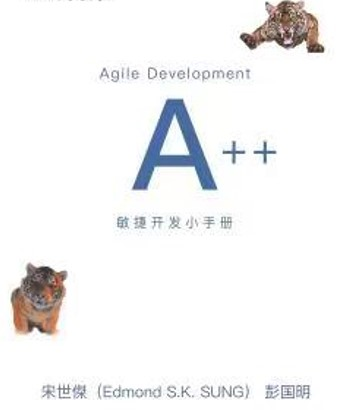
\includegraphics[width=13cm]{aBookCover2latexScreenshot2023-03-08130046.jpg}
\clearpage\newpage \thispagestyle{empty} \mbox{} \cleardoublepage

\thispagestyle{empty} \vspace*{7em}{\centering\Huge A++ 敏捷开发  \par}{\centering -- 从个人提升到 以数据说话 \par}\cleardoublepage

\thispagestyle{empty} \vspace*{\fill} \parbox{.8\textwidth}{\raggedright \scriptsize
\textit{impossible} publisher 2022

printed blindfolded

design: \LaTeX
}
\end{titlepage}
\clearpage \thispagestyle{empty}\cleardoublepage
\newpage % Make sure the following content is on a new page

%----------------------------------------------------------------------------------------
%	TABLE OF CONTENTS
%----------------------------------------------------------------------------------------

\tableofcontents % Prints the table of contents

%----------------------------------------------------------------------------------------
%	INTRODUCTION SECTION
%----------------------------------------------------------------------------------------

%\includeonly(filename,filrname,.......)

%\input(filename)


\chapter*{序} % Introduction chapter suppressed from the table of contents


杨立东 《微管理》作者,四维世景科技(北京)有限公司 总经理

这是一本从事敏捷开发和过程改进的人员的必修之书,作为本书的早期读者,有两个创新让我印象深刻。其一是本书的写法,类似《金刚经》体,全文多是以对话的方式,让读者读起来轻松流畅,少了长篇大论的说教,而是真实和不同IT企业高管、中层、甚至开发团队的问答,在问答中将普遍问题进行归纳总结,并提出解决的方法。其二是案例和数据的引用,虽然很多作者都在书籍中应用案例和大量数据,宋老师则是结合自己多年的从业经验,对案例和数据精益求精,每个案例都颇具经典。通过阅读和理解这些案例,更能体会对话中的问题,以及形成的解决方案的建议。

读过很多管理类的书籍,有些管理数据自始至终贯穿一条主线,例如德鲁克的《卓有成效的管理者》,有些书籍则以故事的形式给企业管理做出启示,例如《目标》。本书的内容始终贯穿过程改进的主题,将宋老师多年在该领域的咨询和培训经验跃然纸上,其中也引用了很多小故事,让书籍活跃了起来,让读者读起来不至于太累。诚然,一千个人有一千个哈姆雷特,具体大家在书籍阅读中去体会吧。

给我感触更深的是宋老师的严谨的写作态度,每次他写完一章,都发给不同的管理者去阅读和提出改进的建议,每次的问题都会得到反馈和在章节中得以应用。这种态度是非常值得尊敬的,毕竟在该领域他才是货真价实的专业人士,而我们这些先期读者只是普通的从业者。

最后,预祝书籍能帮助到那些有志于在管理上提升的从业人员。

\begin{description}
\item[]
\begin{description}
\tightlist
\item[]
2023年3月于北京
\end{description}
\end{description}


\chapter*{感谢 Acknowledgments } % Introduction chapter suppressed from the table of contents

6年前开始把一些培训、评估经验,配合软件工程/项目管理知识,写分享文章,在公司网站和CSDN上发布;2018年在香港教ACP敏捷课也加深了我对敏捷的了解,也发现很多人未了解敏捷开放的重点。初始时候缺乏经验,虽然有些很有趣的题材,但未能组成系列性文章,后面逐步某注销组成系列,分享文章也越来越多被转载。2022年受疫情影响,少出差,可以有更多时间把文章组成书,幸运有各朋友的帮助,终于可以在2023年出版。

非常感谢我的老师、客户、学生和朋友们,如果没有与他们面对面的详细讨论,并在项目过程中反复试验与反馈,不可能写出这本书。这些宝贵经验帮我验证了各种敏捷思路与量化管理的可用性,也让我更加清晰地理解了质量改进的重点。

也感谢朋友圈里各位老师、行业精英们分享经验和意见:其中包括北京的杨立东、王绍军、纪钟涛、武宏伟,天津的韩淑军,上海的周青龙,杭州的胡蕊莉,成都的杨杰等。
感谢杭州的徐洪洋在百忙之中抽空提出了文字上的建议;感谢无锡的陈镜庆、秦瑜不断提出修改意见,并帮助我最后完成本书的编辑;也感谢香港李启良先生对
Mediawiki服务器,Linux,LATEX 等平台的技术支持。%done-1

%\input(xuzhang)

%\chapter*{感谢 Acknowledgments } % Introduction chapter suppressed from the table of contents

6年前开始把一些培训、评估经验,配合软件工程/项目管理知识,写分享文章,在公司网站和CSDN上发布;2018年在香港教ACP敏捷课也加深了我对敏捷的了解,也发现很多人未了解敏捷开放的重点。初始时候缺乏经验,虽然有些很有趣的题材,但未能组成系列性文章,后面逐步某注销组成系列,分享文章也越来越多被转载。2022年受疫情影响,少出差,可以有更多时间把文章组成书,幸运有各朋友的帮助,终于可以在2023年出版。

非常感谢我的老师、客户、学生和朋友们,如果没有与他们面对面的详细讨论,并在项目过程中反复试验与反馈,不可能写出这本书。这些宝贵经验帮我验证了各种敏捷思路与量化管理的可用性,也让我更加清晰地理解了质量改进的重点。

也感谢朋友圈里各位老师、行业精英们分享经验和意见:其中包括北京的杨立东、王绍军、纪钟涛、武宏伟,天津的韩淑军,上海的周青龙,杭州的胡蕊莉,成都的杨杰等。
感谢杭州的徐洪洋在百忙之中抽空提出了文字上的建议;感谢无锡的陈镜庆、秦瑜不断提出修改意见,并帮助我最后完成本书的编辑;也感谢香港李启良先生对
Mediawiki服务器,Linux,LATEX 等平台的技术支持。%done-1

%\input(ganxie)

\chapter*{前言 Prologue} % Introduction chapter suppressed from the table of contents

\begin{quote}
We are uncovering better ways of developing software by doing it and helping others do it.\\
--Agile Software Development Manifesto
\end{quote}

敏捷宣言已经有超过二十年的历史,国内越来越多软件开发团队开始采用敏捷和迭代,但总体效果参差不齐。有些年轻的团队成员听到敏捷不需要文档,以为也不需要注重代码质量,包括代码可读性,导致后面发布的软件产品问题多多,难以维护。要编写出高质量的代码,人本身能力非常关键,但软件工程快速发展,导致编程员人数快速增长,其中很多缺乏专业工程师素养,所有若要敏捷开发真正起作用必须先提升编程员能力。\\
没有数据就无法管理,但很多敏捷团队只是走流程(每天站立会议、看板并非敏捷的重点),缺乏度量,所以管理者一听到敏捷就觉得不靠谱,要求团队用回传统的瀑布开发方式。\\
这二十年来,中外都出版了很多关于敏捷的书,但绝大部分都没有深入去探索以上的问题。这本书就是希望通过解读各种敏捷最佳实践,加上敏捷以外的其他知识,帮助大家理解并更好使用敏捷,提升软件的质量和总生产率,让团队成员与公司管理层获得双赢。\\
同时也希望管理层通过这本书能了解敏捷开发的要素,并能使用敏捷开发模式,帮助公司提升软件产品质量,同时降低成本增加公司的竞争力。\\

\framebox{%
\begin{minipage}[t]{0.97\columnwidth}\raggedright
某技术总监陈总在5天差距分析的最终总结会里问开发团队:

\begin{enumerate}
\tightlist
\item
  你们知道自己是每天产出多少代码行吗?(生产率)
\item
  你们知道平均修复一个系统测试的缺陷花多少工作量(人时)?
\item
  有没有发生过:代码开发完成,系统测试人员尝试运行,但跑不动?(开发人员不能借口说不懂业务,或需求不清,因为你写完代码后,自己连最基本确保代码能运行都没有去做。我还未问你们做开发的有没有做好单元测试/集成测试。)
\item
  你们做测试的知道测试覆盖率是多少?
\end{enumerate}

陈总有丰富开发经验,他最后总结说:
``我以前自己做开发时也是被问过这些问题,我当时也不懂,但我能知耻而后勇------先知道现在的不足,然后按评估老师的最佳实践,持续改进。''\strut
\end{minipage}}

\begin{itemize}
\tightlist
\item
  如果你像陈总下面团队一样,不懂以上问题的答案,这手册可以帮你自己找答案。
\item
  如果你(是管理者或客户/用户)不满意团队的软件开发成果,这手册可以帮你找出根因,启发团队改善。
\item
  如果你已经很了解,恭喜你,但应还可能从这手册里找到一些你未知但有用的方法。
\end{itemize}

\framebox{%
\begin{minipage}[t]{0.97\columnwidth}\raggedright
1980年,STROUSTRUP
先生不满意当时很流行的C语言,因为在70年代,已经有如SmallTalk之类的面向对象语言,C是基于传统步骤式的语言,没有面向对象的功能,所以STROUSTRUP先生就基于C的基础,加上有类功能的C
(C with
Classes)。过了4年,他同事觉得这个名字不好,就改成C++,也出了一本书叫C++,与本来经典的C很相似。后面C++就成为了面向对象的常用语言。\\ A++
继承40年前
C++的思路,希望在敏捷(Agile)开发的基础上,加上增值的元素,更能帮助团队与管理者做好软件开发,让客户满意。\strut
\end{minipage}}
%done-1

%\input(qianyan)

%----------------------------------------------------------------------------------------
%	BOOK PART
%----------------------------------------------------------------------------------------


%\chapter{如何改善敏捷开发质量} % Introduction chapter suppressed from the table of contents


\framebox{%
\begin{minipage}[t]{0.97\columnwidth}\raggedright
按瀑布式阶段开发的困难:\\毕业后参加的开发项目,客户是电信行业,很规范,所以有一定的里程碑和阶段要求。有分析阶段、设计阶段、编码阶段,最后交付,里面当然包括一些测试。\\但往往因为客户的需求不断变化,每一两周都会有新的要求,因为电信业面对的市场变化也很大。导致本来我们预计六个月的项目,后面会有三到四周的测试和调试。也因为不断的有需求变化,不断在修改,几乎就没有时间做好测试,导致为了赶本来合同规定的交付时间,后期不准熬夜加班,更惨的是没来得及测试好,很多代码还是有不少缺陷。\\ 其中一个原因,如果可以把本来前面的设计画UML图的时间省略掉,应该可以腾出更好的时间来做后面的开发和测试。所以当张工开始接触敏捷开发,很相信这种快速交付迭代的方式可以对团队有帮助。\strut
\end{minipage}}

\hypertarget{ux67d0ux8f6fux4ef6ux5f00ux53d1ux516cux53f8ux654fux6377ux5f00ux53d1ux8fc7ux7a0bux6539ux8fdbux6848ux4f8b}{%
\subsection{某软件开发公司敏捷开发过程改进案例}\label{ux67d0ux8f6fux4ef6ux5f00ux53d1ux516cux53f8ux654fux6377ux5f00ux53d1ux8fc7ux7a0bux6539ux8fdbux6848ux4f8b}}

\hypertarget{ux6708}{%
\subsubsection{5月}\label{ux6708}}

张工是公司的中层管理,管理好几个开发团队,有五位项目经理向他汇报。\\
他听说老同学的团队都开始用敏捷开发,很感兴趣,并参加了一些敏捷的交流会,觉得可以解决很多传统瀑布性开发的不足,尤其是可以快速交付给客户。\\
他要求部门经理全面推动敏捷开发,对团队成员进行相关培训,例如,SCRUM Master 内部培训。\\
开始时,张工上级部门经理有些怀疑,问:“后面那些工程文档都不做,会不会影响质量和交付?客户都是专门做电信的,不缺钱,但是对质量要求很高。”\\
张工便解释说,“只要利用敏捷把过程变成迭代,快速交付,改善工程的问题不难,主要是人的问题。”\\
部门经理听到敏捷可以比以前更快速交付,之前客户经常因为延误而不满,他希望可以改变这现状,就答应了。 \\

\hypertarget{ux6708-1}{%
\subsubsection{8月}\label{ux6708-1}}

开发组长王工周五下班后与朋友喝酒,开开心心说: “太兴奋了。研发部门经理决定全面推动敏捷开发SCRUM;我们团队刚参加了两天培训,真正对应我们以前的传统瀑布式开发的种种问题,我们会2周一次迭代,快速反馈,我们会定期小步向客户发版,我们会与用户经常交流,获得他们的反馈。\\
现在团队合作不像以前只按工种工作,也会跟产品经理、业务方面更充分合作,给客户带来更高价值。\\
工作方式也改变了,以前要写需求、规格说明书,现在简单化成用户故事和产品需求卡片,以前我们要做过详细项目计划甘特图,现在用改成用燃烧图和白板。每天用便利贴去写要开发什么东西贴在白板上面,开始的时候,贴的越多感觉越敏捷,我们改成叫 SCRUM team,有一系列的海报围绕我们。我们也没项目经理了,自己管理自己。本来的部门经理现在变成产品负责人,敏捷开发方式让我们团队自己做决策,不仅仅是技术方面,项目相关的也由我们项目组一起讨论决定。\\
解除了以前‘瀑布式开发’的种种烦恼,这一切太完美了。“\\

\hypertarget{ux6708-2}{%
\subsubsection{9月}\label{ux6708-2}}

”你们团队学完敏捷SCRUM后,项目如何?”\\
王工充满自豪地说:\\
“我们培训后就SCRUM的方法,定每两周一个冲刺,每次冲刺前都会用故事点来估算每个功能多大,然后按本次冲刺的资源,估计可以完成多少功能?\\
然后用白板来监控模块完成的情况,哪些在开发中,哪些已经完成,团队和管理者都可以一目了然,不用像以前天天问我们了。我们每天早上也按照SCRUM的规定站立会议,每人说自己完成了哪些任务,今天做什么。\\
大家都很兴奋,确实跟以前瀑布的做法不同。”\\

\hypertarget{ux6708-3}{%
\subsubsection{10月}\label{ux6708-3}}

”你们项目如何?”\\
王工听完,想了一下,然后说:\\
“我们本应上周要完成一次冲刺后的割接上线,但被推到下次了。“\\
”为什么?”\\
王工说: ”我们按培训学到的做冲刺计划会,按照产品的待办事项列表,团队利用扑克牌一起估算每一事项所需要的时间。我们总共八位开发人员,其中有一半是刚毕业不久,但大家刚上完培训,很有信心,虽然技术主管张工对我们出来的估算有些顾虑,觉得我们太理想,但大家刚培训完敏捷,张工也希望让部门经理尽快看到敏捷开发可以加快速度,我们就按这‘进取式’估算开展2周冲刺。\\
但因新人多,编码水平有限,虽然大家已经尽快把开发出来的代码交给系统测试人员手工测试,依据测试发现的缺陷修正再测试,但越来越接近答应客户的2周割接上线时间,但是还是很多BUG没改好,最后几天,基本就天天加班,最终到验收时,仍然有不少问题,最终割接前测试,还是不能达到客户要求的水平,没办法,未能上线。\\
大家确实都尽力冲刺了,但未能达到我们本来希望的结果。“ \\

\hypertarget{ux6708-4}{%
\subsubsection{11月}\label{ux6708-4}}

部门经理之前收到客户总监电话,投诉一些技术缺陷,导致好几次不能按计划上线,问为什么正在交付的软件质量变差了?\\

张工被问到是什么原因时无法回答,只能说立马回去探索原因,尽快汇报,但心里想: “开始敏捷后,因为快速迭代,以前要做概要设计、详细设计的过程反而被忽略了,导致有些写出来的代码,后面就很很难适应快速的变化修改,导致要不然就功能做不出来。 因要赶时间,可以按客户的要求时间交付的话,由于本身代码不好,只可以临时凑凑,不长久。”\\
张工从部门经理办公室出来后,找其中一位项目经理李工喝茶,回顾一下发现项目团队对这次敏捷SCRUM的改革有意见。例如上层为了更快速交付,实现敏捷可以快速交付承诺,把一些本来不太可能的进度时间压到团队去,完全不是本来的那种自主团队管理的概念。出现问题多了,就请了敏捷教练过来辅导,但SCRUM的教练也缺乏软件工程的基础,只懂项目管理过程。所以他们也解决不了软件相关的问题。只是把精益管理怎么做迭代,怎么做回顾这些基本过程再解读一下,解决不了实际问题。\\

李工:
”因为我们做这块业务已经很多年了,本来业务的变化不多,只是一些小的功能改动,所以开发人员尽量不去动核心的代码,怕改动了反而会影响投产,切割不了。但有时为了满足一些新功能,继续在老代码的基础上去写,这种做法效率很低,也不长久,估计一两年后会难以运行了,我们会被迫重写整个产品,而老代码开发人员大部分都离开了,后面的代码维护变得非常困难,即使用敏捷也解决不了这个问题。”\\

无论张工或李工也没有能去总结出什么好的解决方案。现在推行敏捷才刚刚三个月,绝不能打退堂鼓,回到本来的状态。但应怎么解决敏捷带来的问题?挽回部门经理与客户的信心呢?\\
\hypertarget{ux5982ux4f55ux6539ux5584}{%
\subsection{如何改善}\label{ux5982ux4f55ux6539ux5584}}

从以上案例看到,本来管理层希望利用敏捷开发,加快软件开发的交付,减少延误,令客户更满意。但因为只注重项目管理,但没注意和改善软件开发本身的质量,人员能力等因素,开发出来的软件缺陷比以往多,导致后面大量返工,恶性循环,后面更导致延误,最终客户投诉。\\
因为软件本身设计有问题,导致软件难以修改,开发人员都不敢改动任何代码,怕可能会引起系统崩溃。\\

怎样可以确保开发出来软件的质量?\\

敏捷开发有很多种方法(SCRUM 只是其一),因为目的不仅仅是管好项目进度,也要确保软件产品的质量。所以SCRUM 只包括项目管理部分,不全面,反过来,例如极限编程(XP eXtreme Programming),因它的发明者Kent BECK 本身是一位精通面向对象的编程员,所以XP不仅仅关注项目管理,也包含编程的最佳实践。下图是 Ron Jeffery 把XP的重点画成从外到内3层: \\

%\href{文件:cleanagile_f1.8.jpg}{500px}。


\includegraphics[width=10cm]{cleanagile_f18.jpg}

SCRUM 只包含了外层的部分,缺乏中间和内层元素。
按XP的12实践(详见附件)都做到了便可以解决张工的问题吗?\\
不一定。

\framebox{%
\begin{minipage}[t]{0.97\columnwidth}\raggedright Dr
Juran,德鲁克(Drucker)和戴明(Deming)博士是同代人,出生日期相差不超过十年,他们3位都在战后去过日本,帮助日本企业家改善他们的质量。\\在50年代,当德鲁克被ASQ记者问为什么他声称Dr
Juran是现代生产管理之父?\\ 德鲁克解释说:\\现在我们常用的精益(Lean)生产和JIT,其实都是源自Joe
(Joseph Juran)
的过程管理思路,他一直主张要从工作过程入手,从产出反过来决定过程应该如何配合。虽然他没有用"精益"这个词,但他很明白要管理好生产,必须以如何使工人能最好发挥为本,但他这思路被美国很多学术界人士和工业工程师反对:``为什么不是应该由管理者做主,生产者反而成为主角?''\\ 其实戴明、Joe和我都很理解从上而下那一套管理方式是行不通的。日本战后急于回复经济,很接受我们的管理思路,并立马执行,例如丰田40年代未开始推JIT,赶上并超越美国的工业生产。比如我一直和通用汽车(GM)有交流,发现他们就不懂必须先梳理好过程这个概念,从产出反推生产过程应如何配合。尽管GM投入数以亿计的资金自动化信息化,希望改善机器及物流管理,但却不知道本应从过程入手,导致生产到今天也无法追上日本(那套JIT的汽车生产模式)。虽然Joe的思路很清晰,也知道怎么改进企业的质量,可惜一直默默耕耘,没有受到该有的重视。\\ 注:ASQ=American
Society of Quality; JIT=Just-In-Time\strut
\end{minipage}}


下面我们回顾质量大师Dr JURAN 的质量策划方式,如何提升产品质量。\\
客户问:你说Juran先生?\\
我:是的。\\
客户:会不会他的那套质量改进方法太老了,不适用于我们现代。而且他主要关注制作业,不太熟悉我们IT业。\\
我:你听过乔布斯吗?\\
客户:当然听过了,他是苹果创始人。\\
我:乔布斯被苹果赶出来后,自己开创NEXT公司,希望创作未来新一代的电脑产品。他很希望产品在质量方面比较出众。当时,他觉得美国很多企业家都忽略了质量,感觉到被日本的竞争对手赶上。乔布斯便邀请了Dr
Juran从美国东岸飞到西岸,帮他的NEXT公司做辅导,改进过程。(关于他对Dr
Juran的评价,详见附件)

%\href{文件:jobs1Screenshot_2022-06-12_082703.jpg}{100px\textbar{}缩略图}

\includegraphics[width=10cm]{jobs1Screenshot_2022-06-12_082703.jpg}

后面乔布斯回到苹果,大部分NEXT工程师也跟着他一起进入苹果。所以我们现在用一些苹果产品,多多少少都会受当时NEXT质量改进的影响。

我:首先要定义质量是什么?\\

\framebox{%
\begin{minipage}[t]{0.97\columnwidth}\raggedright
质量包括两部分:

\begin{description}
\tightlist
\item[]
满足客户需要 (客户包括外部客户和内部客户)

没有缺陷\\
\end{description}

这定义不仅仅适合于制作业、也适用于服务业,IT业。\\
\strut
\end{minipage}}



我:记得您比较懂财务,对吗?\\
客户:是的,其实我对软件开发还是外行,但较了解财务。\\
我:财务管理是不是包括财务策划、财务监控,财务改进?\\
客户:是的\\
我:Dr
Juran就用财务管理比喻质量管理,同样也有质量策划、质量控制和质量改进。你觉得这个大框架再细分要如何制定质量目标,如何来制定度量等。

%\href{文件:finAnalogyScreenshot_2022-10-07_212149.jpg}{文件:finAnalogyScreenshot
%2022-10-07 212149.jpg}

\includegraphics[width=10cm]{finAnalogyScreenshot_2022-10-07_212149.jpg}

从下表可以看得出来。所以如果我们希望利用敏捷开发,不仅仅是走迭代,确保进度没偏差,还要确保软件产品的质量,也应该用Dr
Juran的质量管理框架去看整个敏捷过程,才能更全面了解如何才可以确保软件开发的质量,也控制好交付工期,不延误,让客户满意。\\
质量策划还包括:

\begin{enumerate}
\tightlist
\item
  设定目标,包括外部和内部目标
\item
  识别内部需求
\item
  依据客户需求制定产品的功能特征
\item
  制定产品和过程的目标
\item
  设计过程来达到这些目标,最后验证过程能力\\
\end{enumerate}

可以用下图了解质量控制和质量改进,比如图的左面就是在过程之前的策划部分。如我们发现缺陷比率为20\%,这就是过程的能力,这个能力是策划的时候已经定好的,过程控制没有什么可以做,只是当缺陷有变化,比如特别高的时候,需要做一些措施返回本来的水平。要改进必须用质量改进,比如希望把缺陷百分比从20\%降到3\%,这就必须驱动一系列的改进计划。改进计划必须要按项目推行执行,没有其它办法。\\
%\href{文件:JuranImprovementScreenshot_2022-10-23_211444.jpg}{500px}

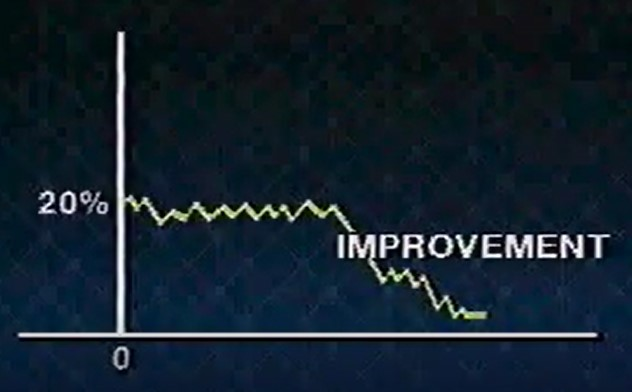
\includegraphics[width=10cm]{JuranImprovementScreenshot_2022-10-23_211444.jpg}

过程改进的计划一般包括:

\begin{enumerate}
\tightlist
\item
  如何识别选择项目。
\item
  组织改进项目的项目团队
\item
  找出缺陷根因
\item
  制定改进措施
\item
  验证是否在真正操作环境里面有效
\item
  处理团队文化上面的抗击阻力
\item
  控制保持本来的水平\\
\end{enumerate}

%\href{文件:IntroXPnJuranStepsScreenshot_2022-10-27_194505.jpg}{550px}

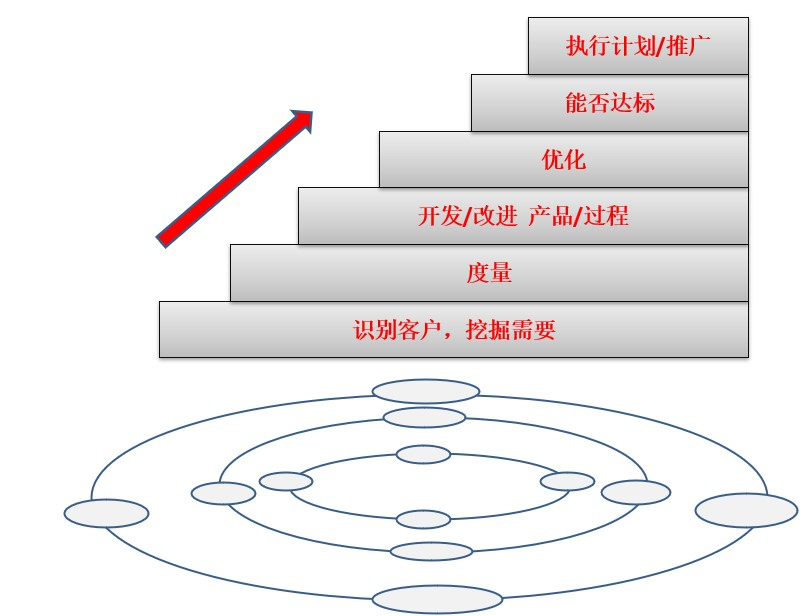
\includegraphics[width=10cm]{IntroXPnJuranStepsScreenshot_2022-10-27_194505.jpg}

客户:你说的策划、控制、改进都挺有道理,但如何跟敏捷,尤其是你说极限编程的实践关联呢?\\
我:任何最佳实践,如果没有定质量目标,配上度量衡量和策划,都只是空想,对长远提升公司文化、团队成员的习惯没有任何帮助。举例:参照上图,例如我们想改善团队的策划和估算。首先要识别客户,哪些是主要干系人
-
甲方有什么要求;内部部门经理,有什么要求。然后从他们的诉求变成过程的功能和特征,但如果特征只是描述,没有数字也没有意义,所以要配合可衡量的度量单位,和用什么方式去收集那些数字,然后依据目标定过程要怎么去做,怎样改。例如

\begin{itemize}
\tightlist
\item
  是否应该从本来的瀑布策划方式制定大的总计划,改用精益的思路,分成迭代,
\item
  每次估算应该怎么做、如何监控等
\item
  然后改进的过程要不断从实验中优化
\item
  最后还要用数字证明这改善比本来好,然后在其他团队全面推广\\
\end{itemize}

而不是单纯`空降'某敏捷流程(例如 SCRUM),便能加快团队的发布速度。
所以虽然极限编程里每一条实践都是最佳实践,也必须配合质量策划,和监控改进才会有效果。

\framebox{%
\begin{minipage}[t]{0.97\columnwidth}\raggedright
很多人都知道戴明环代表PDCA(Plan-Do-Check-Act),其实持续改进的道理也不是戴明博士发明,Juran
对它的了解与应用不会比戴明差。\strut
\end{minipage}}

要注意在整个过程里,高层起非常关键的作用:\\
所以Dr
Juran强调高层不能把公司的质量工作下放(例如,由某助手负责)。我们的经验就是这种做法往往导致最后质量不会有任何改进。原因很简单,每位中层管理者都有一定的KPI标准,资源也是固定的。如果这些没有根本的改变,质量是不会提升,因为整个管理环境没有变化,项目经理、部门经理还是会按以前的做法继续操作,不会听高层的口号或宣传,很快整个质量改进将会失败而终,所有的活动尤其质量相关的,高层必须亲身参与。包括制定质量目标,参与质量提升的高层委员会,定期监督进展等。

这手册会:

\begin{itemize}
\tightlist
\item
  先从个人如何提升,与自我管理开发过程开始
\item
  然后以团队如何做好迭代回顾(复盘)为改进试点\\
\end{itemize}

利用实际案例让大家了解如何开展过程改进。\\
然后,针对每条XP实践,探索如何能在团队里用上,并能改善开发产品的质量(降低客户缺陷密度)。\\
改进都要有衡量才具体,``度量与分析''部分会从基础概念开始,探索如何建立标杆(基线)与预测模型。\\

\hypertarget{ux9644ux4ef6}{%
\section{附件}\label{ux9644ux4ef6}}

\hypertarget{xp}{%
\subsection{XP}\label{xp}}

\hypertarget{ux7f16ux7801ux5b9eux8df5-coding-practices}{%
\subsubsection{编码实践 Coding
Practices}\label{ux7f16ux7801ux5b9eux8df5-coding-practices}}

\hypertarget{cp1ux7b80ux5355ux5730ux7f16ux7801ux548cux8bbeux8ba1-code-and-design-simply}{%
\paragraph{CP1:简单地编码和设计 Code and Design
Simply}\label{cp1ux7b80ux5355ux5730ux7f16ux7801ux548cux8bbeux8ba1-code-and-design-simply}}

\begin{itemize}
\tightlist
\item
  To produce software that is easy to change 使软件易于更改
\end{itemize}

\hypertarget{cp2ux65e0ux60c5ux5730ux91cdux6784-refactor-mercilessly}{%
\paragraph{CP2:无情地重构 Refactor
Mercilessly}\label{cp2ux65e0ux60c5ux5730ux91cdux6784-refactor-mercilessly}}

\begin{itemize}
\tightlist
\item
  To find the code's optimal design 找到代码的最佳设计
\end{itemize}

\hypertarget{cp3ux5236ux5b9aux7f16ux7801ux6807ux51c6-develop-coding-standards}{%
\paragraph{CP3:制定编码标准 Develop Coding
Standards}\label{cp3ux5236ux5b9aux7f16ux7801ux6807ux51c6-develop-coding-standards}}

\begin{itemize}
\tightlist
\item
  To communicate ideas clearly through code 通过代码清晰地传达想法
\end{itemize}

\hypertarget{cp4ux5171ux540cux7684ux8bcdux6c47-develop-a-common-vocabulary}{%
\paragraph{CP4:共同的词汇 Develop a Common
Vocabulary}\label{cp4ux5171ux540cux7684ux8bcdux6c47-develop-a-common-vocabulary}}

\begin{itemize}
\tightlist
\item
  To communicate ideas about code clearly 清楚传达软件设计的想法
\end{itemize}

\hypertarget{ux5f00ux53d1ux5b9eux8df5-develop-practices}{%
\subsubsection{开发实践 Develop
Practices}\label{ux5f00ux53d1ux5b9eux8df5-develop-practices}}

\hypertarget{dp1ux6d4bux8bd5ux9a71ux52a8ux5f00ux53d1tdd-test-driven-development}{%
\paragraph{DP1:测试驱动开发TDD
Test-Driven-Development}\label{dp1ux6d4bux8bd5ux9a71ux52a8ux5f00ux53d1tdd-test-driven-development}}

\begin{itemize}
\tightlist
\item
  To prove that code works as it should 来证明软件正常工作:\\
\end{itemize}

\begin{description}
\tightlist
\item[]
- Test-first programming(prim practice\#)
\end{description}

\hypertarget{dp2ux7ed3ux5bf9ux7f16ux7a0b-pair-programming}{%
\paragraph{DP2:结对编程 Pair
Programming}\label{dp2ux7ed3ux5bf9ux7f16ux7a0b-pair-programming}}

\begin{itemize}
\tightlist
\item
  To spread knowledge, experience and ideas 传播知识、经验和想法:\\
\end{itemize}

\begin{description}
\tightlist
\item[]
- Pair Programming(prim practice\#)
\end{description}

\hypertarget{dp3ux96c6ux4f53ux8d1fux8d23ux5199ux597dux4ee3ux7801vs-ux53eaux987eux8651ux81eaux5df1ux7684ux4ee3ux7801-collective-code-ownership-vs-individual-own-code}{%
\paragraph{DP3:集体负责写好代码(vs 只顾虑自己的代码) Collective Code
Ownership (vs individual own
code)}\label{dp3ux96c6ux4f53ux8d1fux8d23ux5199ux597dux4ee3ux7801vs-ux53eaux987eux8651ux81eaux5df1ux7684ux4ee3ux7801-collective-code-ownership-vs-individual-own-code}}

\begin{itemize}
\tightlist
\item
  To spread the responsibility for the code to the whole team
  将写好代码的责任扩展到整个团队:\\
\end{itemize}

\begin{description}
\tightlist
\item[]
- Whole team(prim practice\#)

- Share code(corollary practice\#)
\end{description}

\hypertarget{dp4ux6301ux7eedux96c6ux6210-integrate-continually}{%
\paragraph{DP4:持续集成 Integrate
Continually}\label{dp4ux6301ux7eedux96c6ux6210-integrate-continually}}

\begin{itemize}
\tightlist
\item
  To reduce the impact of adding new features 降低添加新功能的影响:
\end{itemize}

\begin{description}
\tightlist
\item[]
- Incremental Design(prim practice\#)

- Single code base(corollary practice\#)

- Ten-minute Build(prim practice\#)

- Continuous Integration(prim practice\#)
\end{description}

\hypertarget{ux5546ux52a1ux5b9eux8df5-business-practices}{%
\subsubsection{商务实践 Business
Practices}\label{ux5546ux52a1ux5b9eux8df5-business-practices}}

\hypertarget{bp1ux5c06ux5ba2ux6237ux6dfbux52a0ux8fdbux56e2ux961f-add-a-customer-to-the-team}{%
\paragraph{BP1:将客户添加进团队 Add a Customer to the
Team}\label{bp1ux5c06ux5ba2ux6237ux6dfbux52a0ux8fdbux56e2ux961f-add-a-customer-to-the-team}}

\begin{itemize}
\tightlist
\item
  To address business concerns accurately and directly
  准确、直接地解决业务问题:
\end{itemize}

\begin{description}
\tightlist
\item[]
- Real Customer involvement(corollary practice\#)
\end{description}

\hypertarget{bp2ux8ba1ux5212ux6e38ux620f-play-the-planning-game}{%
\paragraph{BP2:计划游戏 Play the Planning
Game}\label{bp2ux8ba1ux5212ux6e38ux620f-play-the-planning-game}}

\begin{itemize}
\tightlist
\item
  To schedule the most important work 安排最重要的工作:\\
\end{itemize}

\begin{description}
\tightlist
\item[]
- Weekly cycle ; Quarterly cycle ; Slack (prim practice\#)
\end{description}

\hypertarget{bp3ux5b9aux671fux53d1ux5e03-release-regularly}{%
\paragraph{BP3:定期发布 Release
Regularly}\label{bp3ux5b9aux671fux53d1ux5e03-release-regularly}}

\begin{itemize}
\tightlist
\item
  To return the customer's investment often
  尽早交付,让客户看到投资回报:
\end{itemize}

\begin{description}
\tightlist
\item[]
- Incremental Deployment(corollary practice\#)

- Daily Deployment(corollary practice\#)
\end{description}

\hypertarget{bp4ux4ee5ux53efux6301ux4e45ux7684ux901fux5ea6ux5de5ux4f5c-work-at-a-sustainable-pace}{%
\paragraph{BP4:以可持久的速度工作 Work at a Sustainable
Pace}\label{bp4ux4ee5ux53efux6301ux4e45ux7684ux901fux5ea6ux5de5ux4f5c-work-at-a-sustainable-pace}}

\begin{itemize}
\tightlist
\item
  To go home tired, but not exhausted 回家时虽然很累,但不筋疲力尽:\\
\end{itemize}

\begin{description}
\tightlist
\item[]
- Slack (prim practice\#)
\end{description}

\hypertarget{ux4e54ux5e03ux65afux8c08dr.juran}{%
\subsection{乔布斯谈Dr.Juran}\label{ux4e54ux5e03ux65afux8c08dr.juran}}

\framebox{%
\begin{minipage}[t]{0.97\columnwidth}\raggedright
他(NEXT CEO)接受访谈时,对美国企业,质量,和 Dr.Juran
观点的重点内容:\\
美国已经富裕了很多年。很多企业都忘记要获得成功,还是要关注基本功,包括教育。现在我们美国很多企业面临困难,处处感觉被日本领先了。其实不是日本针对我们,而是我们作为美国企业家应反思一下,为什么我们的战略比他们差,为什么我们的策划不如日本?我们知道Dr.Juran
在40/50年代多次去日本,帮助日本企业提升质量。现在他回到美国,希望把他的经验带到美国企业,提升竞争力,可以再一次成为世界第一。

我觉得Dr.Juran
很实在,不是泛泛而谈。我们的工程师也深受他这种风格影响。无论我们之中谁问他问题,总裁还是工程师,他都会全心全意用自己的知识解答。所以工程师和我都很希望用他那套方法来做提升。整个质量提升的道理其实很简单,是一个重复的过程,然后我们需要不断去看,有哪些无效的环节要省略,哪部分要重新设计,不断试验、提升,就这么简单。重点是所有的提升都应该是科学化的,有数据而不是泛泛而谈。

一般管理层的思路是:我是领袖,你们应该听我命令。但应该是反过来,让应如何做好的决定权利放在团队手上,做改进不需要请求管理层的批准。改进是工作的一部分,整个架构扁平化,自己管控日常过程,每位工程师应像以前的工匠,愿意花精力不断做好。然后能以自己最后做出的优质工艺、产物自豪。\strut
\end{minipage}}%done-1

\part{案例分析}

\chapter{如何改善} % Introduction chapter suppressed from the table of contents

\hypertarget{ux654fux6377ux5f00ux53d1ux8fc7ux7a0bux6539ux8fdbux6848ux4f8b}{%
\subsection{敏捷开发过程改进案例}\label{ux654fux6377ux5f00ux53d1ux8fc7ux7a0bux6539ux8fdbux6848ux4f8b}}

\hypertarget{ux6708}{%
\subsubsection{5月}\label{ux6708}}

A公司一直专门为某电信公司提供针对客服、线上播放等业务。\\
张工是公司的中层管理者,管理好几个开发团队,有5位项目经理向他汇报。\\
他听说老同学的团队都开始用敏捷开发,很感兴趣,便参加了几次敏捷交流会,觉得可以解决很多开发团队的问题,尤其是可以快速交付给客户。\\
他便提建议给部门经理推动敏捷开发,找咨询公司做相关培训,例如SCRUM Master 内部培训,然后全面开展实施。\\
开始时,部门经理有些怀疑,问:“听起来很吸引,但后面那些工程文档都不做,会不会影响质量和交付?客户都是专业做电信的,不缺钱,但是对质量要求很高。”\\
张工解释说:“只要利用敏捷把过程变成迭代,快速交付、改善工程的问题不难,主要是人的问题。”\\
部门经理听到敏捷可以比以前更快速交付,因之前客户经常抱怨项目延误,他也希望可以改变,就答应了。 \\

\hypertarget{ux6708-1}{%
\subsubsection{8月}\label{ux6708-1}}

开发组长王工,三十出头,毕业后一直做开发,一年前晋升为组长。周五下班后与朋友喝酒,很开心地说: “太兴奋了。我们团队刚参加了两天SCRUM 培训,并指出我们以前按传统瀑布式开发的种种问题。我们会两周一次迭代并割接上线,还会与用户代表定期交流,不再会像以前几个月交付后才发现开发出来的功能不合需求。\\
现在团队合作不像以前只按工种工作,也会跟产品经理、业务方面更充分合作,给客户带来更高价值。\\
工作方式也会改变,以前要写需求、规格说明书,现在简单化成产品需求卡片,以前我们要做详细项目计划和甘特图。现在会改成用燃烧图和“KANBAN”。 每天用便利贴去写要开发什么内容贴在白板上面,我们会改成叫SCRUM Team。工作区周围都有SCRUM 的海报,提醒我们SCRUM的重点。团队也没项目经理了,自己管理自己。部门经理会变成产品负责人,敏捷开发方式让我们团队自己做决策,不仅仅是技术方面,项目相关的也由我们项目组一起讨论决定。”\\

\hypertarget{ux6708-2}{%
\subsubsection{9月}\label{ux6708-2}}

王工的朋友老杨周五晚喝酒时问他:”你们团队使用敏捷SCRUM后,效果如何?”\\
王工立马面露笑容,充满自信地跟大家说:“我们培训后就使用SCRUM的方法,每2周一个冲刺,每次冲刺前都会用故事点来估算每个功能多大,然后按本次冲刺的资源,估计可以完成多少功能。然后用看板来监控模块完成的情况,哪些正在开发中?哪些已经完成?团队和管理者都可以一目了然,不用像以前......。”\\
“听你这样说,我也要尽快提议领导引入敏捷开发。”\\
“我还未说完,我们每天早上也按照SCRUM的规定站立会议,每人说自己完成了哪些任务,今天做什么......。” 

\hypertarget{ux6708-3}{%
\subsubsection{10月}\label{ux6708-3}}

喝酒时老杨问王工:“你们项目如何?”\\
王工听完,没有立马回应,把注意力放在窗外的大街上,想了一下,然后说:“我们本应上周要完成一次冲刺后的割接上线,但被推到下次了。”\\
“为什么?”\\
王工说:“我们按培训学到的做冲刺计划会议,按照产品的待办事项列表,团队利用扑克牌一起估算每一事项所需要的时间。我们总共8位开发人员,其中有一半是刚毕业不久,但大家刚上完培训,很有信心,虽然技术主管张工对我们出来的估算有些顾虑,觉得我们太理想,但大家刚培训完敏捷,张工也希望让部门经理尽快看到敏捷开发可以加快速度,我们就按这‘进取式’估算开展两周冲刺。但因新人多,编码水平有限,虽然大家已经尽快把开发出来的代码交给系统测试人员手工测试,依据测试发现的缺陷修正再测试,但割接上线期限前4天还有很多Bug没改好,最后3天,基本是天天加班,最终到上线期限仍然有不少问题,最终割接前测试,还是不能达到客户要求的水平,没办法上线。大家确实都尽力冲刺了,但未能达到我们本来希望的结果。”\\
“你们开发人员在提交代码到系统测试之前,有没有自己先自测?”\\
王工说:“我们敏捷开发每天早上站立会议上都用看板,记录每个模块的进度完成情况,开发编码人员都说自测过。”\\
“如果开发人员能自己把握好交付代码的质量。不应该等到系统测试才发现这么多问题要解决。你们团是怎么做自测?有记录吗?”\\
王工说:“这我就没有详细问了,因为我们学完SCRUM后,大家更关注开发速度,用看板保证按计划的进度,不延误。但没想到后面缺陷会这么多。而且有些问题改完以后还会导致另外一些Bug发生。到了最后,因为赶时间,大家对修改Bug已经麻木了。”\\
“你们之前不是都有代码评审和扫描的习惯吗?”\\
王工说:“之前我们确实比较多评审,除了评审核心设计和代码,我们还要求组长抽查新人开发的代码,并且要求提交代码前必须通过扫描。但我们为加快速度,没有硬性要求必须先通过扫描。经你一问,我想这也可能是出现很多Bug的原因之一。”\\
“你们有没有事后迭代复盘?复盘可以帮团队分析之前有哪些不足,后面改进。”\\
王工说:“我们都交付不了,哪里有心情来做回顾、复盘。最后几天冲刺,大家每天都没睡好,大家都只想回去好好睡一觉。”\\

\hypertarget{ux6708-4}{%
\subsubsection{11月}\label{ux6708-4}}

部门经理之前收到客户总监电话,投诉一些技术缺陷,导致好几次不能按计划上线,问为什么正在交付的软件质量变差了?\\
张工被问到是什么原因时无法回答,只能说立马回去探索原因,尽快汇报。\\
张工从部门经理办公室出来后,找其中一位项目经理李工喝茶,问他对今次敏捷改革的意见。\\
两人都赞同敏捷开发应能帮助团队提升,当张工问李工有什么可以改善的地方,李工说:“让团队自主是件好事,但因为我们专注做这块业务已经很多年了,本来业务的变化不多,只是一些功能微调,所以开发人员尽量不去修改核心代码,怕改动了反而会影响投产,无法切割。为了不触及原始代码,新代码都只能在核心的外围去写,但这种做法效率很低,无法有效长久维持,到时会被迫重写整个产品。而且懂老代码的开发人员大部分都离开了,代码维护越来越困难。\\
敏捷教练强调团队自主管理,给团队空间发挥。但SCRUM的教练缺乏软件工程的基础,只懂项目管理过程。所以他们也解决不了软件相关的问题。只是把精益管理怎么做迭代、怎么做回顾这些基本过程再解读一下,解决不了实际问题。''\\
张工说:``很赞同,这是必须要解决的问题。但现在燃眉之急是要解决主管提出的客户投诉不能按时交付这紧急问题。不然我们以后也不敢再提敏捷开发了。''\\
无论张工或李工也没有能去总结出什么好的解决方案。现在推行敏捷才刚刚3个月,绝不能打退堂鼓,回到本来的状态。但应怎么解决敏捷带来的问题,挽回部门经理与客户的信心呢?\\

从上面的SCRUM案例看到,本来管理层希望利用敏捷开发,加快软件开发的交付、减少延误、令客户更满意。但因为只注重项目进度是否延误,但团队没注意如何改善软件开发本身的质量,也因为团队成员能力不足,开发出来的软件缺陷比以往还多,导致后面大量返工,恶性循环,后面更导致延误和客户投诉。\\
因为软件本身设计有问题,导致软件难以修改,开发人员都不敢改动任何代码,怕可能会引起系统崩溃。\\
怎样可以确保开发出来软件的质量?\\
敏捷开发有很多种方法(SCRUM只是其一),因为目的不仅仅是管好项目进度,也要确保软件产品的质量。所以SCRUM只包括项目管理部分,不全面。反过来,例如极限编程(XP
eXtreme Programming),因它的发明者Kent Beck
本身是一位精通面向对象的编程员,所以XP不仅仅关注项目管理,也包含编程的最佳实践。下图是Ron
Jeffery 把XP的重点画成从外到内3层:

%\href{文件:cleanagile_f1.8.jpg}{500px}。

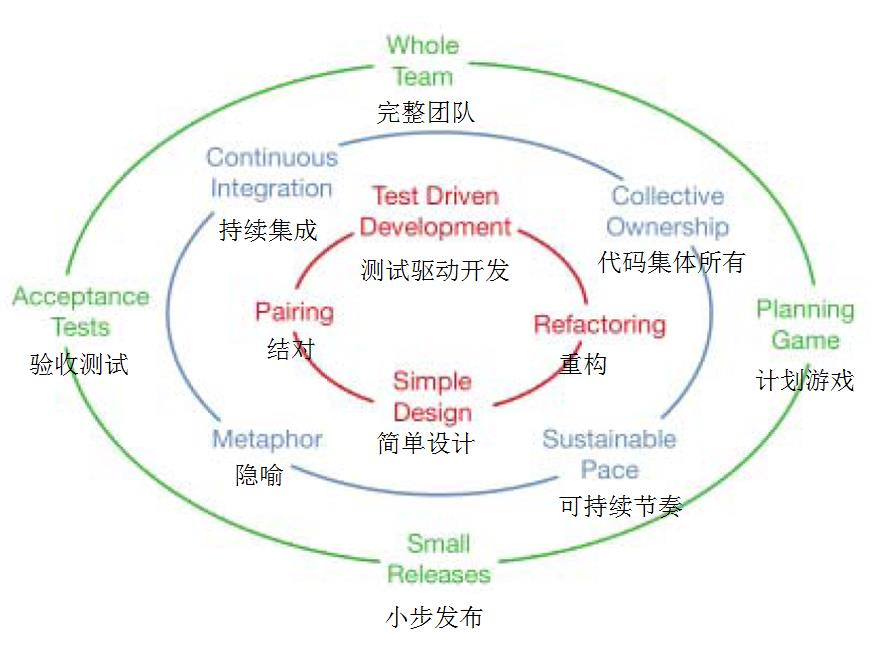
\includegraphics[width=6cm]{Cleanagile_f181.jpg}

SCRUM只包含了外层的部分,缺乏中间和内层元素。
按XP的12实践(详见附件)都做到了便可以解决张工的问题吗?\\

\hypertarget{ux5982ux4f55ux6539ux5584}{%
\subsection{如何改善}\label{ux5982ux4f55ux6539ux5584}}

既然SCRUM方法有不足,XP方法能解决开发质量问题,是否团队学好XP便能帮助团队做好敏捷开发? 怎样才能不断完善?\\
先问你以下关于汽车公司的问题:

%\href{文件:TvsGcompScreenshot_2023-06-07_121806.jpg}{650px}

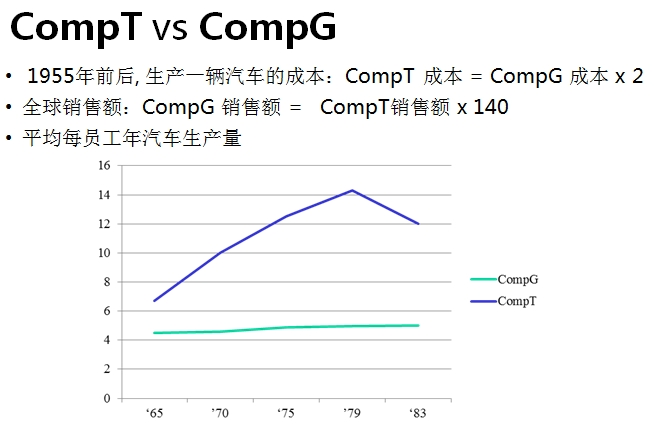
\includegraphics[width=6cm]{TvsGcompScreenshot_2023-06-07_121806-1.jpg}

T公司在60年代,在销售、生产成本都远远不如G公司,但它每年生产率都一直提升。请猜猜T和G是那家公司?
(提示:两家都是世界级汽车公司,现在你还能买到它们生产的汽车。)

\begin{description}
\item[]
\begin{description}
\tightlist
\item[]
= = = = = = = = = = = =
\end{description}
\end{description}

G 是美国通用,T是日本丰田。\\
为什么丰田能从一家战后小公司提升为世界最大(\#)的汽车公司?

\begin{description}
\item[]
\begin{description}
\tightlist
\item[]
(\# :
2023年底,总收入可能是大众第一、丰田第二,但丰田销售数量世界第一。)
\end{description}
\end{description}

\hypertarget{ux4e30ux7530ux6545ux4e8b}{%
\subsection{丰田故事}\label{ux4e30ux7530ux6545ux4e8b}}

%\href{文件:ToyotaPresidentPicture1.png}{200px}\\

%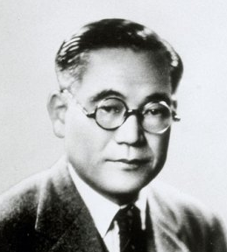
\includegraphics[width=6cm]{ToyotaPresidentPicture1.png}
%丰田喜一郎先生 (创始人)\\
%\href{文件:大野耐一.png}{200px}

%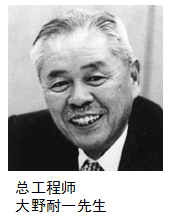
\includegraphics[width=6cm]{大野耐一.png}

二战后50年代,丰田汽车规模很小,经营很困难,在破产边缘。
但丰田创始人喜一郎先生明白美国生产线的弊端,意识到未来的汽车生产必须是Just-In-Time:

\begin{itemize}
\tightlist
\item
  每一辆都是按客人订单订制:例如,颜色,配置,左右钛等。
\item
  从钢材原料开始,整个生产线零等待、零浪费。
\end{itemize}

\begin{description}
\item[]
\begin{description}
\tightlist
\item[]
每个工作步骤所需配件按生产需要到达(不晚到也不早到),把生产过程中的配件降到零。
\end{description}
\end{description}

%\url{文件:远景1.png}

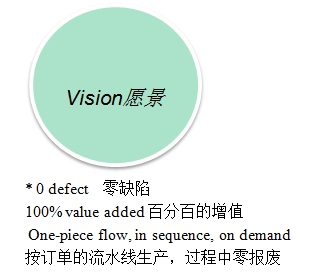
\includegraphics[width=6cm]{远景1.png}

喜一郎先生安排总工大野耐一去美国汽车公司考察。

\framebox{%
\begin{minipage}[t]{0.97\columnwidth}\raggedright
为什么福特Model-T 出名?\\它是第一辆一般人买得起的汽车
首辆现代汽车是由德国奔驰(Benz)于1885制作,
但是这些第一代汽车都非常昂贵。\\
老福特是一名工程师,对机械特别感兴趣,
白天是爱迪生公司的总工程师,到了下班后就研究汽车发动机
经过十年的不断优化,最终开发出4冲程自动汽车发动机 他的发明大大降低了汽车组件的成本 1908
Model-T 首次推出市场,售价是850美金,虽然已经比同期的其他厂家汽车便宜,
但还是超出一般工人家庭可以负担的水平。

为了进一步降低成本,老福特觉得必须想其他办法。
汽车组装一直都是作坊式运作, 所以组装汽车需要超过12个工时。
为了降低组装时间,必须要学其他工厂,
如啤酒,麦粉厂,它们都已经是流水式生产线生产(Assembly Line)
福特把整个Model-T组装拆分成84步骤, 并培训工人只做一项工作,
还聘用了科学工程师Taylor先生设计整个流程,提高效率,最终可以一个半小时完成组装一辆汽车。\\
生产线生产帮助福特公司把成本和售价降下来, 在15年期间(1913 ~
1927),福特公司总共生产了15,000,000辆 Model-T。
虽然大量生产能直接降低生产成本, 但这种做法也要付出代价:

\begin{itemize}
\tightlist
\item
  为了生产所有都是同一个款式同一个颜色,黑色
\item
  为了提高生产的效率,也增加了组件的库存量
  (为了提高效率,降低成本,大部分组件都要批量生产(Batch
  production),例如轮胎。例如上面右下图看到工厂里存在大量轮胎。)
\end{itemize}

%\href{文件:FordModelT_2023-06-10_100431.jpg}{600px}

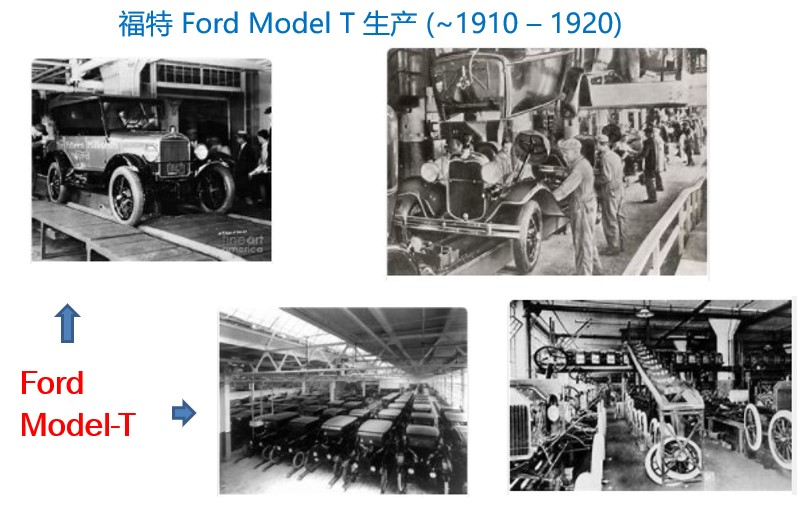
\includegraphics[width=6cm]{FordModelT_2023-06-10_100431.jpg}

\strut
\end{minipage}}

\textbf{Federick Taylor 与科学管理(Scientific Management)}\\
%\href{文件:Weisbord_P34.jpg}{200px}

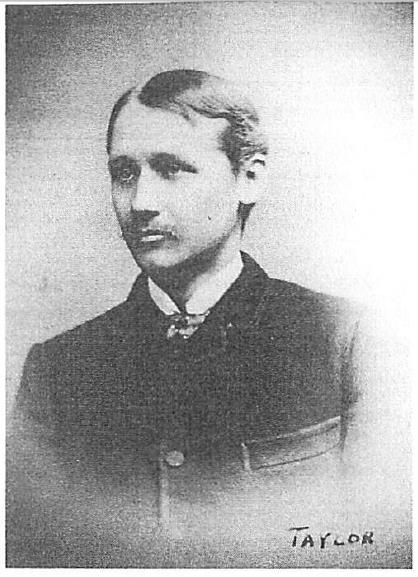
\includegraphics[width=6cm]{Weisbord_P34.jpg}

\framebox{%
\begin{minipage}[t]{0.97\columnwidth}\raggedright
十九世纪末美国很多工业快速扩张,Taylor先生发现当时很多工厂生产力很低,例如钢铁厂。
他是很落地、实干的人,他就想有什么好方法可以让提高生产力,工人也多赚些钱。他发现很多工作都未设计好,未能好好利用工人,他针对工作本身做很多科学研究,测量每个工作应该多长时间,怎么做最好,然后按他的最佳设计把工作细分,也同时要求公司提高员工的奖励,希望工人看到因科学管理,提高生产,个人也受益。1890年,他加入了Bethlehem
Steel,钢铁业的大公司,帮它设计了很多奖励制度,也设定了一些叫工业工程师(Industrial
engineers)岗,发现生产力可以提升30-40\%。后来公司被收购,他也被辞退,他便成为顾问,当时都没有顾问这个职业,他可算是全球首位工程顾问。
\strut
\end{minipage}}

总工大野耐一先生从美国的超市(非汽车公司)得到如何做Just-In-Time的启发,回国后就开始在丰田全力推动。开始时,很多人都觉得Just-In-Time
这个愿景好像是远不可及的梦想。而到了今天,现代汽车生产都基本做到了当年喜一郎先生和大野耐一先生的梦想。(详见附件)

\hypertarget{ux6c34ux9762ux4e0bux7684ux7ba1ux7406ux601dux8def}{%
\subsection{水面下的管理思路}\label{ux6c34ux9762ux4e0bux7684ux7ba1ux7406ux601dux8def}}

%\url{文件:冰山.png}

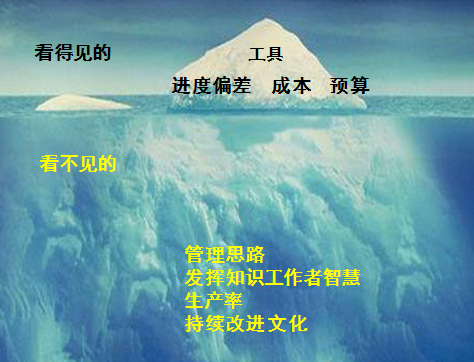
\includegraphics[width=6cm]{冰山.png}

为什么丰田能成功地把汽车生产做到 Just-In-Time
,超越西方的巨头,使日本汽车制造过程成为世界``标准''?\\
但我们不能单从表面看这``系统''的方法和技巧,例如大家都熟悉的看板管理(他的竞争对手通用、福特肯定都学过),更重要是了解背后的管理思路。我们看看下面丰田七个习惯,开始了解水面下的``系统'':\\


\begin{enumerate}
\tightlist
\item
  容易实现的目标不是好目标
\item
  不以``我们公司''作主语
\item
  重复五遍“为什么”
\item
  持续改善没有停止
\item
  成长比成功更重要
\item
  以忙碌为耻
\item
  从心里相信``大家的力量''
\end{enumerate}

\hypertarget{ux5bb9ux6613ux5b9eux73b0ux7684ux76eeux6807ux4e0dux662fux597dux76eeux6807}{%
\subsubsection{容易实现的目标不是好目标}\label{ux5bb9ux6613ux5b9eux73b0ux7684ux76eeux6807ux4e0dux662fux597dux76eeux6807}}

\textbf{\texttt{不是“削减一成”,而是通过“取消一个零”来发现浪费}}

``如何把原先需要三小时的工作,改用三分钟完成''\\
如果听到上司以上要求,你该怎么回答呢?如你回答:``这太强人所难了''、``绝对做不到'',请读以下丰田案例。\\
\{\textbar{} class="wikitable" \textbar{}\textbf{``单分换模(Single
Minute Exchange of Die)''}例子:\\
1965年,丰田汽车在推行丰田生产方式时遭遇一个瓶颈:装置更换时间太长,其中特别是500吨冲压机和1000吨冲压机的模具,更换时间长达2\textasciitilde{}4小时。如果不缩短这两个模具的更换时间,就不可能实现多品种少量生产方式。\\
挑战由大野耐一先生统领,在生产管理的先行者,新乡重夫先生的指导下,分两个阶段展开。\\
改善开始之前,新乡先生凭借自己多年的工作经验,了解到装置更换有两种方式:\\
①内部装置更换------必须在机器停下来以后,才能进行的装置更换。\\
②外部装置更换------能在机器运转过程中,或是在运转起来以后,进行的装置更换。\\
要缩短时间,把内部装置更换和外部装置更换清楚地分开来是一个关键。能在外部装置替换作业中进行的工作,就全部在外部装置替换过程中实施。同时,分别对内部装置替换和外部装置替换进行改善。通过这种方法,装置更换时间缩短为一个半小时。\\
完成这一改善花费了半年时间。通常能有这样的成果就可以告一段落了。但是,大野先生仍要求进一步缩短时间。\\
他要求把更换过程``缩短为3分钟!''通常通过改善能把原先的2\textasciitilde{}4小时缩短为一个半小时,就可以很满意地说``已经很好了''。但是,大野先生不这么想。他认为:
``既然能缩短到这个水平,那么继续改善肯定可以把时间缩短为3分钟。''\\
\textbf{改变汽车生产的单分换模的秘密}\\
对于这一要求,在以新乡先生为中心的技术小组中,自然有人提出``3分钟绝对干不完''。但是,新乡先生认为:
``如果能把内部装置更换全部转化为外部装置更换,
3分钟也不是不可能......''\\
之后,他着手对多达100个以上的项目进行了改善。\\
首先,进一步对内部装置更换和外部装置更换进行细分,彻底把内部装置更换转化为外部装置更换。同时,想方设法对各种切割工具和模具进行设置,使得更换时用一个动作即可完成。此外,在紧固件上也动了很多脑筋。这样,终于创造出了无数项不花时间、能够简单完成同时可以在作业时保持稳定的改善。\\
紧接着,对作业顺序反复进行改善,实施标准化(制订没有多余工序的作业标准)。这样,在挑战进行了三个月后的某一天,真的只要3分钟就能完成了!这个结果让所有人都大吃一惊。\\
\textbar{}\}

\hypertarget{ux6807ux6746ux7ba1ux7406-benchmarking}{%
\paragraph{标杆管理
(Benchmarking)}\label{ux6807ux6746ux7ba1ux7406-benchmarking}}

很多公司都会用百分比来设定改善目标,但改善了百分比,不一定代表质量有改善,例如某快递公司去年送包裹未按时送达占8\%,今年是6\%,好像已经改善了2\%。但去年托运的数量是500万件,所以8\%是4万件。今年的数量是750万件,所以今年的6\%就是4万5千件。\\
所以今年包裹延误增加了5000,这样非但没有任何改善,反而服务变得更差了。所以更重要是看数字本身。容易达到的目标,不是好目标。所以丰田一般会选行业里最强的对手作为基准(标杆)。\\
1965年,美国通用汽车公司是世界顶尖。例如销售额的规模,丰田与通用是1:60,完全不在同一个层次上。成本上丰田对通用是1:0.5,成本是通用的两倍。\\
丰田把当时顶尖的通用公司当成了自己进行标杆管理的对象。\\
如果丰田某零件的成本价格是1000日元,通用是400日元。丰田会把通用的400日元,作为基准成本价,把原料价定为400日元,把差额600作为``不必要花费'',让团队立马改善,尽早达到标杆。\\
丰田(如下图)很注重各种标杆,例如内部标杆、竞争性标杆等。软件开发也应该同样利用数据来制订量化目标。

%\url{文件:丰田p1.png}

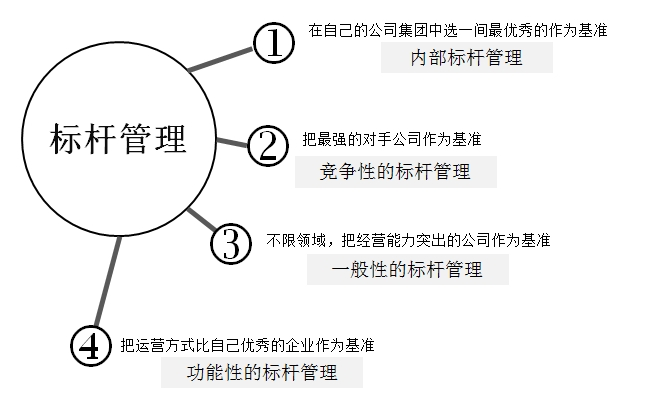
\includegraphics[width=6cm]{丰田p1.jpg}

\framebox{%
\begin{minipage}[t]{0.97\columnwidth}\raggedright
某家专门开发金融软件产品的公司:

研发总监问我“你接触这么多国内的企业,觉得有哪家优秀的,可以作为我们的标杆? 我们尝试寻找,但还未找到。有些优秀的公司,但它们业务跟我们不同,我们产品是面对企业,也非嵌入式软件(我们不生产硬件)。”\\
“确实难找,我真没遇到过,但为什么你只看国内公司?” 
\strut
\end{minipage}}

从以上对话看到越来越多高水平开始用标杆管理,但标杆必须是比自己高很多才有作用。

\hypertarget{ux4e0dux4ee5ux6211ux4eecux516cux53f8ux4f5cux4e3bux8bed}{%
\subsubsection{不以``我们公司''作主语}\label{ux4e0dux4ee5ux6211ux4eecux516cux53f8ux4f5cux4e3bux8bed}}

\begin{itemize}
\tightlist
\item
  不是从``专业''的角度,而是从``顾客''的角度生产产品。
\end{itemize}

\begin{description}
\tightlist
\item[]
创业大忌------闭门造车,所以丰田的原则,对客户有用就一定做出来,但对客户无用或者不想要,就绝不生产。\\
\end{description}

%\url{文件:丰田p3-1.jpg}

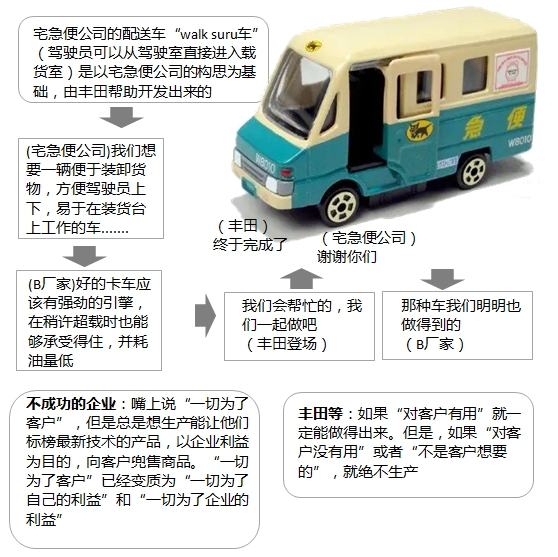
\includegraphics[width=6cm]{丰田p3-1.jpg}

要创新必须从``顾客''的角度看,不单从工程师的视角看不仅适用于丰田和汽车制造:

\framebox{%
\begin{minipage}[t]{0.97\columnwidth}\raggedright
征服太空,踏上月球。 六七十年代,美国开始阿波罗太空计划。
首批宇航员强烈要求工程师加上窗户、逃生门、可人手控制等
(现代我们会觉得这些是太空船 (spacecraft) 基本要求, 但当时是闻所未闻)。

1980,一位NASA工程师回顾当时工程部的想法:
``你们又不是火箭专家,航天专家,只是飞行员。
希望可以在火箭驾驶舱人工控制火箭飞行,开玩笑!
太极端,你们可不了解成本多高,我们应可以很轻易用工程的理由拒绝。''
\strut
\end{minipage}}

\hypertarget{ux91cdux590dux4e94ux904dux4e3aux4ec0ux4e485-why}{%
\subsubsection{重复五遍``为什么''(5
Why)}\label{ux91cdux590dux4e94ux904dux4e3aux4ec0ux4e485-why}}

最重要的不是追究责任而是找出根因。

五个``为什么''是一种找根因的方法,实例可详见附件:

\begin{itemize}
\tightlist
\item
  不停留在``原因''上,而要找出``真因'',彻底改善。
\item
  不追究责任,而是追究原因。
\end{itemize}

丰田要求检查人员不仅仅检查过程与结果,做统计报告,交给负责的工程师,也必须分析产生不合格的原因,使同类的问题不再发生。
检查人员不仅仅是``考官'',也作为``内部教练'',指导生产的持续改善。

反过来,如果下属因出错,导致失败,立马被上司骂,觉得很难受,就会从反省变为排斥。
如果公司有这种``责难,追究责任''的风气,坏消息就会被隐瞒。所以丰田有一条原则是``Hard
news first (先说坏消息)''。

当工程师找出了问题就必须要求他查找原因、提供数据,但很多时候这个工作并不简单,但大野耐一先生决不放弃,必须找到根因。他说:\emph{做到一半是不行的,只有一个期限
--------- ``到完成为止''}

\hypertarget{ux6301ux7eedux6539ux5584ux6ca1ux6709ux505cux6b62}{%
\subsubsection{持续改善没有停止}\label{ux6301ux7eedux6539ux5584ux6ca1ux6709ux505cux6b62}}

\framebox{%
\begin{minipage}[t]{0.97\columnwidth}\raggedright
A公司用丰田方式进行了两年多的生产改革,高层觉得成果令人瞩目,举办改善报告会,邀请集团内其他公司高层来参加。\\
在参观工厂时,A公司的负责人利用图表展示如何成功地缩短了零件替换时间。C公司高层听了说明后问:``你说把90分钟缩短为了30分钟,最初的一年半,你们确实一口气实现了时间的缩短,但是,看一下这半年,你们好像只缩短了几分钟。对于这点,你是怎样考虑的呢?''\\
开始实施改善后的一年左右,成果会很快出现。因为以前有问题的地方太多,所以值得改善的地方多不胜数,只要努力实施改善,零件替换时间、库存、生产效率等等,各方面都会眼看着变得越来越好。但是,到达某个水平以后,改善的步伐经常就会停止下来。\\
到了这个阶段以后,有很多企业都会因为``改到这样已经很不错了''而停止改革的脚步。\\
着手执行丰田式的改革方式本身并不是一件太难的事。只要解决问题,就可以获得成果。难的是,必须要把改善持续搞下去。\\
人有的时候很想``往前跑'',但有的时候也想``停下来休息''。对丰田而言,比起以为``已经胜利了''而在睡午觉的兔子而言,他们更推崇不倦不怠一直向前进的乌龟。\\
报告会结束的时候,A公司的员工说:``课题依旧堆积如山。我们的目标是成为世界一流的工厂,所以我们会永远改善下去''这也是A公司全体员工的心声。听到此,
B公司和C公司的高层也总算放下心来了。
\strut
\end{minipage}}

能否坚持下去是能否成功的关键因素。

\hypertarget{ux6210ux957fux6bd4ux6210ux529fux66f4ux91cdux8981}{%
\subsubsection{成长比成功更重要}\label{ux6210ux957fux6bd4ux6210ux529fux66f4ux91cdux8981}}

\begin{itemize}
\tightlist
\item
  要培养人才,``改变体制''比``改变人''更有效。\\
\end{itemize}

有些工厂只依赖张贴标语、海报,希望可以减少工地的事故发生率,但丰田不注重喊口号,而是动手干实事,包括机械保安、设备保安等。

%\href{文件:ft_223.1.png}{500px}

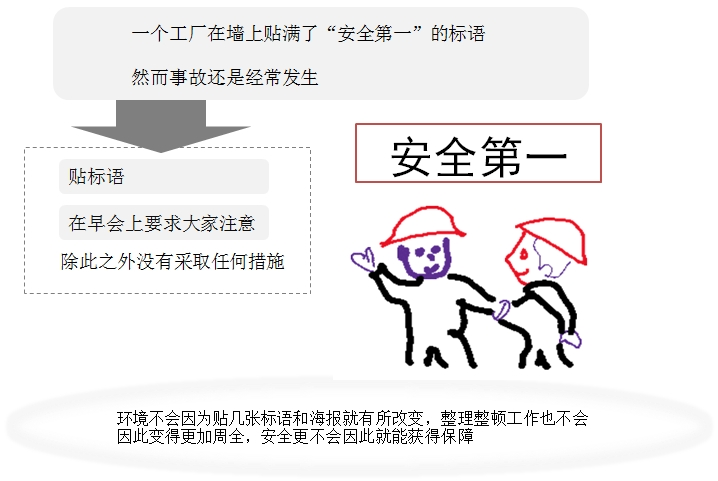
\includegraphics[width=6cm]{Ft_223111.jpg}

所谓5S
指的是:整理、整顿、清扫、清洁及修养。无法做到这些基本原则的企业及个人是无法生产出优质产品。\\
在这些基本原则中,丰田尤其注重``整理和整顿''。\\
``处理掉不需要的东西是整理。使得任何时候都能把想要的东西拿出来的叫整顿。只是把东西放整齐的则叫做排列。我们要求在生产现场必须要做好整理和整顿。''\\
实例:

\framebox{%
\begin{minipage}[t]{0.97\columnwidth}\raggedright
B
先生受命去子公司A公司实施重建工作。当他第一天到达工厂的时候,他看到的是一副脏得无法形容的情景。机器上布满了油和灰尘,地板和墙壁上沾满污渍。飞散开来的机油上又落了灰尘,积成厚厚的一层。半成品和零件随便地东一堆西一堆地放着,工具扔得到处都是。工厂里想找块站的地方都很困难。这样的状态不用说也会降低丰田的``开动率''。仓库里也是堆满了零件和产品,但看那样子就知道,若要问起某个东西在哪里的话是不会有人知道的。\\
他在晨会上问大家: ``你们想带自己的家人或恋人来这个工厂吗?''\\
A公司的员工们一直戒备着从总公司来的B先生新官上任后不知道会烧什么火,听到这句话后面面相觑。看来B先生好像对工厂的这个样子很不满意,他们一个个相视苦笑。就在大家不出声苦笑的过程中,不知道是谁轻轻说了一句``怎么可能带他们来呢''。声音虽然不大,但是B先生却没有漏听掉。``为什么不想带自己最亲近的人来看一看你们工作的地方呢?''``这么脏,哪好意思给人看啊。''``那为什么就让它一直这么脏着呢?''\\
这样追问以后,B先生听到了很多理由。``太忙了,没时间打扫''、``没有打扫的工具''、``没钱买重新粉刷的油漆''、``收拾好以后马上又脏了,扫了也是白搭''......。\\
``心情''改变工作

在B先生听来,这些理由中其实就蕴含了``改善的线索''。\\
每当人们不想干什么事的时候,就会想出理由来辩解为什么干不了。大部分人都会因为这样的理由,而在是否要行动时犹豫再三。\\
但是,
B先生身体力行丰田方式。他认为,找借口不如去思考该如何做。``用思考借口的脑袋来想怎么做'',
``借口''其实和``之所以能做到的理由''是一致的。\\
B先生逐一攻破了A公司员工的``做不到的理由''。``没有时间''他就在工作时间中拿出几分钟将其设定为``清洁时间''。没有打扫工具和油漆,他就早早地买好。对于员工所说的``白搭'',
B先生身先士卒地去捡垃圾、擦墙壁。\\
没过多久,原本很脏的工厂开始慢慢干净起来了。而当工厂开始变干净以后,员工们都产生了一种要把这种干净的状态维持下去的心情。他们开始自己收拾机器的漏油,而当初觉得``扫了也是白搭''的员工开始觉得``打扫也是件不坏的事''。\\
随着工厂开始变得干净起来,业绩也开始恢复了。工作的环境变好以后,在那里工作的人心情也就会随之出现了变化。
\strut
\end{minipage}}

大野耐一在他的《现场经营》中写过:

\framebox{%
\begin{minipage}[t]{0.97\columnwidth}\raggedright
如果仅仅觉得(机器人)用起来很方便,或是能代替我去工作,那就说明根本还没有能够有效地使用机器人。如果引进机器人,就要从引进的那一刻起对机器人进行改善,或者要使自己的做法能和机器人合拍。\\
如果公司老有人在嘀咕做这样的事买个机器人回来就成了,甚至在不明白目前的情况下有没有比引进机器人更好的方法,就成天想着如果不买机器人,改善就不可能进行得下去,那么,这家企业就糟糕了。首先要弄清楚目前企业里的机器能做到哪一步,或是为了使现在的机器能发挥更大的作用,而先充分地去使用现在的机器。这样当以后有先进的机器引进来的时候,就可以依靠其获得``基于智慧的+α''(注)了。丰田最终决定要在最后的组装工序中引进机器人也是经过了一段很长的准备期的。\\
比如说公司计划要把过去由自动机械完成的作业换成由机器人来完成。一般的做法无非就是直接用机器人把自动机械替换掉。但是,丰田首先挑选出典型的生产线,将这条生产线上原本由自动机械干的工作暂时换为人工作业。以此来详细地分析人会采用什么样的方法去做。并执行彻底的作业改善。在此基础上,探讨有什么工作是机器人做得了的,又有什么是机器人做不了的,以及为什么做不了。有的情况下还特意开发一些更容易能和机器人配合得起来的零件。他们是在经过了这样的过程以后,才和机器人的生产商共同开发,并最终决定导入机器人的。\\
实行机器人化并不是为了能够减少人数。在丰田不但``人的工作与机械(机器人)的工作''泾渭分明,而且两者的存在很和谐,推行机器人化是为了能让人去做附加值更高的工作。\\

\begin{description}
\tightlist
\item[]
(注:α指不仅要以现在的技术、价格、服务等为基准进行标杆管理,还必须预想一个包含了将来的变化的``现在+α'',作为标杆管理的对象。
)
\end{description}\strut
\end{minipage}}

第一个例子,说明工作环境的重要性,主管通过逐步改善工厂的环境,团队的士气与生产率都提升了。\\
从第二个例子看到成长不是仅仅按既定方向去做,必须思考动脑筋,并了解背后的目的才能真正取得效果。\\
这些丰田的成长故事也适用于软件开发团队,例如,有些软件开发团队盲目地想推自动化测试,却没有想好哪一类测试应自动化,哪一类更合适手工测试,最后因效果与投入不匹配,以失败告终。

\hypertarget{ux4ee5ux5fd9ux788cux4e3aux803b}{%
\subsubsection{以忙碌为耻}\label{ux4ee5ux5fd9ux788cux4e3aux803b}}

\begin{itemize}
\tightlist
\item
  不吝惜智慧,但要吝惜汗水
\end{itemize}

\framebox{%
\begin{minipage}[t]{0.97\columnwidth}\raggedright
\textbf{把``动作''转变为 ``工作''}
以前,当大家批评某机关的工资太高时,职员会以上班时间很长,
``一直在努力工作''为由来反驳人们的批评。这其实是一种对于``有动作''和``在工作''的混淆。不管上班时间有多长,如果没能够创造出利润,那么就不能称之为工作,也不能称之为一直在努力。\\
丰田是把``动作''和``工作''分开考虑的。在丰田看来,``就算一直在动也不代表那个人在工作''。省掉徒劳动作,把``在动着''转化为``在工作''。\\
大野耐一先生曾经问过年轻员工:
``每天工作一小时左右,你们能做到吗?''\\
听了这句话后,有人抱怨:``算上加班时间,我们一天工作9个小时,他那句话是什么意思?''\\
确实,他们在公司待了很长时间,但如果把``有动作''和``在工作''分开考虑,9个小时中,真正在工作的时间可能只有1小时。大野先生指的是这一点。\\
关键的不在于流着汗在公司转了多长时间,而要把自己的工作区分成``徒劳作业''和``有价值作业''。
\strut
\end{minipage}}

\framebox{%
\begin{minipage}[t]{0.97\columnwidth}\raggedright
二战后,日本经济萎缩,丰田辞退了不少员工。1950年,朝鲜战争爆发,需要大量增产,但丰田选择了只增加设备,而不增加人手,大野先生也借这机会,完善丰田生产方式,成功找到了以不增加人手为前提的增产办法。
\strut
\end{minipage}}

\hypertarget{ux4eceux5fc3ux91ccux76f8ux4fe1ux5927ux5bb6ux7684ux529bux91cf}{%
\subsubsection{从心里相信``大家的力量''}\label{ux4eceux5fc3ux91ccux76f8ux4fe1ux5927ux5bb6ux7684ux529bux91cf}}

\begin{itemize}
\tightlist
\item
  不是靠``一个不平凡的人'',而是依靠``一百个平凡人''来创造亮眼的成绩。
\item
  生产产品就是培养人才。
\end{itemize}

\begin{description}
\tightlist
\item[]
``做事业最关键是人.......`培养人才'为基础''总裁丰田英二先生。
\end{description}

\begin{description}
\tightlist
\item[]
有一位丰田员工被问到``丰田生产方式到底是什么''的时候,这样回答:
``就是在人的智慧建起的基础上,立起了自动化和及时生产这两根支柱。''\\

他所说的``人的智慧''是指``在一线工作人员的智慧''。\\
\end{description}

\framebox{%
\begin{minipage}[t]{0.97\columnwidth}\raggedright
\textbf{人了不起的智慧}\\
所谓丰田生产方式其实就是要建立起一种体制,把``人了不起的智慧''引导出来,使得这些智慧能在生产一线得到充分发挥。所以说``丰田生产方式源自人的智慧''。
\strut
\end{minipage}}

企业相信员工的智慧提升以后,员工们的干劲、使命感、责任感都会随之而生,最重要的是,员工们会因此逐渐对工作抱有自豪感。一旦员工们的意识改变了,理所当然地,企业的竞争力也将获得很大的提高。\\
大野耐一先生说:``改良是指通过投入资金使情况变好,
改善是指通过动脑筋使情况变好。''

\framebox{%
\begin{minipage}[t]{0.97\columnwidth}\raggedright
{带诚意去赢得协作}\\
B先生所在的A公司曾以丰田生产方式为基础进行了生产改革。\\
 要进行生产改革没有技术部门的配合是行不通的。但是,任凭
B先生怎么要求,技术部门依然毫不合作。B先生实在没有办法了,只能向总裁要求:
``请加大我手上的权力,让我可以支配技术部。''总裁回答:
``你去给我请教了大野(耐一)先生以后再说!''\\
 于是B先生去找大野先生,在听他诉说了自己面临的窘境以后,大野先生对他说:
``你这一两天跟我一起去工厂转转吧!''并于百忙之中抽出时间带B先生参观了丰田的工厂以及附近的协作企业的工厂。这期间,大野先生什么话都没说,只在第二天下午问B先生:``怎么样,你明白了吗?''\\
 B先生回答:
``我觉得在工厂听到的关于厂长的改善事例,跟丰田方式所强调的重点好像不太一致。''听了B先生的回答以后,大野先生点头:
``就连我,也是一直都在忍耐的啊。工作并不是有权力就能解决问题的。要想得到对方的理解和信任,拿出诚意去找人家吧。''\\
 从那以后,
B先生再也不找``因为我手里没有权力''之类的借口,而总是带着诚意去找对方协商,不久以后,他成功地对A公司实施了生产改革。\\
 每当听到有人感慨``下属不听话''的时候,一位曾在丰田工作的人就会说:
``你要求自己的孩子"每天学习三小时'时,他会听话去学习吗?''\\
 对方的回答是:
``估计没用。''\\
 ``连自己的孩子都这样,更何况那些成年的员工呢?''
\strut
\end{minipage}}

%学员下午做互动练习时便说自己公司里确实有不少“河马”横行。\\
%从以上两故事看到,优秀的公司高层,无论东西方,都理解公司的发展依赖“大家的力量”和各人的智慧,同心协力,“大王”文化会妨碍公司持续改进,难以改善。 

\hypertarget{ux6539ux5584ux8d28ux91cf}{%
\subsection{改善质量}\label{ux6539ux5584ux8d28ux91cf}}

质量管理与财务管理类似,同样也有质量策划、质量控制和质量改进,基于这大框架再细分:如何制订质量目标、度量等。\\
质量策划包括:

\begin{enumerate}
\tightlist
\item
  设定目标,包括外部和内部目标。
\item
  识别内部需求。
\item
  依据客户需求制订产品的功能特征。
\item
  制订产品和过程的目标。
\item
  设计过程来达到这些目标,并验证过程能力。\\
\end{enumerate}

\textbf{质量控制和质量改进}\\
下图的左面是在过程之前的策划部分,例如发现缺陷比率为20\%,这就是过程的能力,这是策划的时候已经定好的,过程控制没有什么可以做,只是当缺陷有变化,比如特别高的时候,需要做一些纠正措施。例如希望把缺陷从20\%降到3\%,这就必须驱动一系列的改进计划。改进计划也必须按项目管理方法推行与监控,没有其他办法。\\
%\href{文件:JuranImprovementScreenshot_2022-10-23_211444.jpg}{500px}

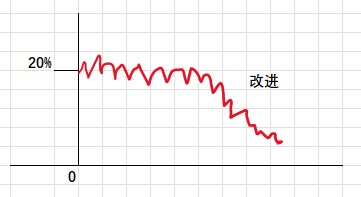
\includegraphics[width=6cm]{JuranImprovementScreenshot_2022-10-23_211444-1.jpg}\\

所以如果希望敏捷开发有效,不仅仅是走迭代过程,确保进度没偏差,还要确保软件产品质量,也应该用裘兰博士的质量管理思路去看敏捷过程,才能更全面了解如何确保软件开发的质量,控制交付工期。\\
最佳实践,如果没有质量目标、度量衡量和策划,都只是空想,对长远提升企业文化、员工素质没有任何帮助。\\
例如我们想改善团队的策划和估算。首先要识别客户,哪些是主要干系人——甲方有什么要求、内部部门经理有什么要求。然后从他们的诉求变成过程的功能和特征,但如果特征只是描述,没有数字也没有意义,所以要配合可衡量的度量单位,和用什么方式去收集那些数字,然后依据目标定过程要怎么去做,怎样改。\\
不是单纯``空降''某敏捷流程(例如SCRUM),便能加快团队的发布速度。
所以虽然极限编程里每一条实践都是最佳实践,也必须配合质量策划,和监控改进才会有效果。

乔布斯85年离开苹果,自己开创NEXT公司,他很注重质量,便邀请了裘兰博士 (Dr
Juran)从美国东岸飞到西岸,帮他们公司做辅导,改进过程。以下是节录他接受访谈时,对美国企业、质量和裘兰博士的观点:

\framebox{%
\begin{minipage}[t]{0.97\columnwidth}\raggedright
美国已经富裕了很多年。很多企业都忘记要获得成功,还是要关注基本功,包括教育。现在我们美国很多企业面临困难,处处感觉被日本领先了。其实不是日本针对我们,而是我们作为美国企业家应反思一下,为什么我们的战略比日本差,为什么我们的策划不如日本?我们知道裘兰博士多次去日本,帮助日本企业提升质量。现在他回到美国,希望把他的经验带到美国企业,提升竞争力,可以再一次成为世界第一。

我觉得裘兰博士很实在,不是泛泛而谈。我们的工程师也深受他这种风格影响。无论我们之中谁问他问题,总裁还是工程师,他都会全心全意用自己的知识解答。所以工程师和我都很希望用他那套方法来做提升。质量提升的道理其实很简单,是一个重复的过程,然后我们需要不断去看,有哪些无效的环节要省略,哪部分要重新设计,不断试验、提升,就这么简单。重点是所有的提升都应该是科学化的,有数据而不是泛泛而谈。

一般管理层的思路是:我是领袖,你们应该听我命令。但应该是反过来,让应如何做好的决定权利放在团队手上,做改进不需要请求管理层的批准。改进是工作的一部分,整个架构扁平化,自己管控日常过程,每位工程师应像以前的工匠,愿意花精力不断做好。然后能以自己最后做出的优质工艺、产物自豪。

\strut
\end{minipage}}

\hypertarget{ux7ed3ux675fux8bed}{%
\subsection{结束语}\label{ux7ed3ux675fux8bed}}

按质量大师裘兰博士定义,质量包括两部分:

\begin{itemize}
\tightlist
\item
  满足客户需要(包括外部客户和内部客户)
\item
  没有缺陷\\
\end{itemize}

这定义不仅仅适合于制造业,也适用于服务业、IT业。\\
丰田生产方式是TQM (Total Quality
Management全面质量管理)的最佳例子,TQM强调专注客户、持续改进、以数据说话、员工参与等,丰田生产方式覆盖了TQM原则的七项(除了战略)。

%\href{文件:TQM_1.2.png}{500px}

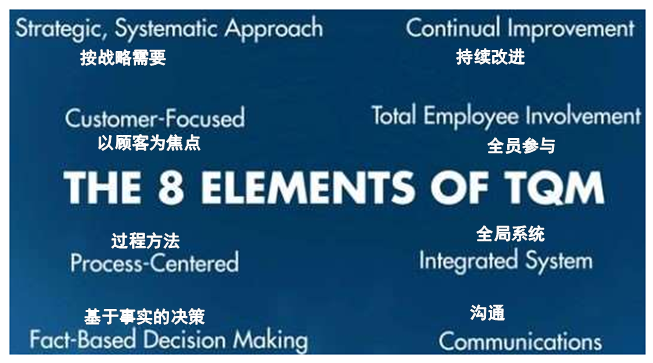
\includegraphics[width=6cm]{TQM_12.png}

从以上丰田故事看到丰田方式如何帮公司培养知识工作者,发挥人的无限智慧,
为公司增值。\\
丰田汽车,从50年代开始,沿用裘兰博士的质量管理思路,成为世界最大的汽车企业。\\
针对软件开发,如何基于以上质量管理、精益管理思路,配合敏捷开发最佳实践,提升产品质量与团队竞争力?\\
所以团队成员,包括团队组长与组员的能力是过程改进的基础,不仅仅依赖领导。\\
虽然XP比SCRUM更全面列出敏捷团队的最佳实践,但还必须依赖团队持续改善才会有效果。\\
下一部分,我们探索``团队与自我改善基本功''与成功要素。

\hypertarget{ux9644ux4ef6}{%
\section{附件}\label{ux9644ux4ef6}}

\hypertarget{ux73b0ux4ee3ux6c7dux8f66ux751fux4ea7}{%
\subsection{现代汽车生产}\label{ux73b0ux4ee3ux6c7dux8f66ux751fux4ea7}}

今天Just-In-Time已成为汽车制造的主流,例如:日产在英国牛津郡(Oxfordshire)专门生产mini
车的 工厂便能做到:

\begin{itemize}
\tightlist
\item
  从钢材原料到生产出汽车只需要24小时。
\item
  整个生产线没有任何中间等候,每68秒出一辆。
\item
  每天生产1000辆车。
\end{itemize}

%\href{文件:NissanRobots-OIP.h8UAC7FBjlaCmA_mBepJjQHaEi.jpg}{500px}\\
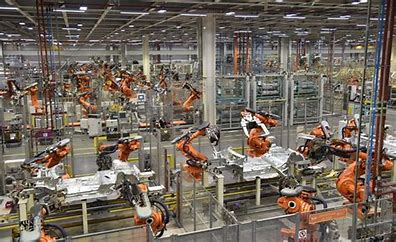
\includegraphics[width=6cm]{NissanRobots-OIPh8UAC7FBjlaCmA_mBepJjQHaEi.jpg}\\
\textbf{挑战}:每一辆汽车都不同 ------颜色、设备、左右驾驶座等

\begin{itemize}
\tightlist
\item
  生产线上每一辆汽车都按照客户需求订制。
\item
  组件不早不晚按需求准时到达生产线。
\item
  这便需要信息化系统把客户订单转换成生产信息。
\end{itemize}

%\href{文件:NissanJIT_OIP.RQGKy67DWGTu-DQiOCqW2gHaEK.jpg}{500px}
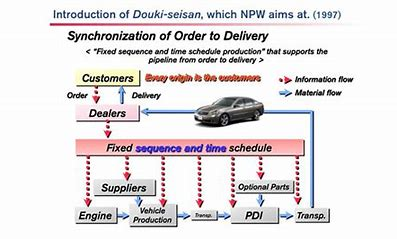
\includegraphics[width=6cm]{NissanJIT_OIPRQGKy67DWGTu-DQiOCqW2gHaEK.jpg}\\

例如生产线上每一辆的颜色都可以不同:\\
%\href{文件:NissanProdLineOIP.wJFmfMl7q2_V8JaQi4kQ8QHaE6.jpg}{400px}\\
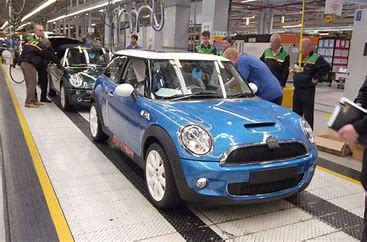
\includegraphics[width=6cm]{NissanProdLineOIPwJFmfMl7q2_V8JaQi4kQ8QHaE6.jpg}\\

\hypertarget{xp}{%
\subsection{XP}\label{xp}}

\hypertarget{ux7f16ux7801ux5b9eux8df5coding-practices}{%
\subsubsection{编码实践(Coding
Practices)}\label{ux7f16ux7801ux5b9eux8df5coding-practices}}

\hypertarget{cp1ux7b80ux5355ux5730ux7f16ux7801ux548cux8bbeux8ba1code-and-design-simply}{%
\paragraph{CP1:简单地编码和设计(Code and Design Simply
)}\label{cp1ux7b80ux5355ux5730ux7f16ux7801ux548cux8bbeux8ba1code-and-design-simply}}

\begin{itemize}
\tightlist
\item
  To produce software that is easy to change 使软件易于更改
\end{itemize}

\hypertarget{cp2ux65e0ux60c5ux5730ux91cdux6784-refactor-mercilessly}{%
\paragraph{CP2:无情地重构 (Refactor
Mercilessly)}\label{cp2ux65e0ux60c5ux5730ux91cdux6784-refactor-mercilessly}}

\begin{itemize}
\tightlist
\item
  To find the code's optimal design 找到代码的最佳设计
\end{itemize}

\hypertarget{cp3ux5236ux8ba2ux7f16ux7801ux6807ux51c6-develop-coding-standards}{%
\paragraph{CP3:制订编码标准 (Develop Coding
Standards)}\label{cp3ux5236ux8ba2ux7f16ux7801ux6807ux51c6-develop-coding-standards}}

\begin{itemize}
\tightlist
\item
  To communicate ideas clearly through code 通过代码清晰地传达想法
\end{itemize}

\hypertarget{cp4ux5171ux540cux7684ux8bcdux6c47-develop-a-common-vocabulary}{%
\paragraph{CP4:共同的词汇 (Develop a Common
Vocabulary)}\label{cp4ux5171ux540cux7684ux8bcdux6c47-develop-a-common-vocabulary}}

\begin{itemize}
\tightlist
\item
  To communicate ideas about code clearly 清楚传达软件设计的想法
\end{itemize}

\hypertarget{ux5f00ux53d1ux5b9eux8df5-develop-practices}{%
\subsubsection{开发实践( Develop
Practices)}\label{ux5f00ux53d1ux5b9eux8df5-develop-practices}}

\hypertarget{dp1ux6d4bux8bd5ux9a71ux52a8ux5f00ux53d1tdd-test-driven-development}{%
\paragraph{DP1:测试驱动开发TDD (Test-Driven-Development
)}\label{dp1ux6d4bux8bd5ux9a71ux52a8ux5f00ux53d1tdd-test-driven-development}}

\begin{itemize}
\tightlist
\item
  To prove that code works as it should 来证明软件正常工作:\\
\end{itemize}

\begin{description}
\tightlist
\item[]
- Test-first programming(prim practice\#)
\end{description}

\hypertarget{dp2ux7ed3ux5bf9ux7f16ux7a0b-pair-programming}{%
\paragraph{DP2:结对编程 (Pair
Programming)}\label{dp2ux7ed3ux5bf9ux7f16ux7a0b-pair-programming}}

\begin{itemize}
\tightlist
\item
  To spread knowledge, experience and ideas 传播知识、经验和想法:\\
\end{itemize}

\begin{description}
\tightlist
\item[]
- Pair Programming(prim practice\#)
\end{description}

\hypertarget{dp3ux96c6ux4f53ux8d1fux8d23ux5199ux597dux4ee3ux7801vs-ux53eaux987eux8651ux81eaux5df1ux7684ux4ee3ux7801-collective-code-ownership-vs-individual-own-code}{%
\paragraph{DP3:集体负责写好代码(vs 只顾虑自己的代码) Collective Code
Ownership (vs individual own
code)}\label{dp3ux96c6ux4f53ux8d1fux8d23ux5199ux597dux4ee3ux7801vs-ux53eaux987eux8651ux81eaux5df1ux7684ux4ee3ux7801-collective-code-ownership-vs-individual-own-code}}

\begin{itemize}
\tightlist
\item
  To spread the responsibility for the code to the whole team
  将写好代码的责任扩展到整个团队:\\
\end{itemize}

\begin{description}
\tightlist
\item[]
- Whole team(prim practice\#)

- Share code(corollary practice\#)
\end{description}

\hypertarget{dp4ux6301ux7eedux96c6ux6210-integrate-continually}{%
\paragraph{DP4:持续集成( Integrate
Continually)}\label{dp4ux6301ux7eedux96c6ux6210-integrate-continually}}

\begin{itemize}
\tightlist
\item
  To reduce the impact of adding new features 降低添加新功能的影响:
\end{itemize}

\begin{description}
\tightlist
\item[]
- Incremental Design(prim practice\#)

- Single code base(corollary practice\#)

- Ten-minute Build(prim practice\#)

- Continuous Integration(prim practice\#)
\end{description}

\hypertarget{ux5546ux52a1ux5b9eux8df5-business-practices}{%
\subsubsection{商务实践 (Business
Practices)}\label{ux5546ux52a1ux5b9eux8df5-business-practices}}

\hypertarget{bp1ux5c06ux5ba2ux6237ux6dfbux52a0ux8fdbux56e2ux961f-add-a-customer-to-the-team}{%
\paragraph{BP1:将客户添加进团队( Add a Customer to the Team
)}\label{bp1ux5c06ux5ba2ux6237ux6dfbux52a0ux8fdbux56e2ux961f-add-a-customer-to-the-team}}

\begin{itemize}
\tightlist
\item
  To address business concerns accurately and directly
  准确、直接地解决业务问题:
\end{itemize}

\begin{description}
\tightlist
\item[]
- Real Customer involvement(corollary practice\#)
\end{description}

\hypertarget{bp2ux8ba1ux5212ux6e38ux620f-play-the-planning-game}{%
\paragraph{BP2:计划游戏 (Play the Planning
Game)}\label{bp2ux8ba1ux5212ux6e38ux620f-play-the-planning-game}}

\begin{itemize}
\tightlist
\item
  To schedule the most important work 安排最重要的工作:\\
\end{itemize}

\begin{description}
\tightlist
\item[]
- Weekly cycle ; Quarterly cycle ; Slack (prim practice\#)
\end{description}

\hypertarget{bp3ux5b9aux671fux53d1ux5e03-release-regularly}{%
\paragraph{BP3:定期发布 (Release
Regularly)}\label{bp3ux5b9aux671fux53d1ux5e03-release-regularly}}

\begin{itemize}
\tightlist
\item
  To return the customer's investment often
  尽早交付,让客户看到投资回报:
\end{itemize}

\begin{description}
\tightlist
\item[]
- Incremental Deployment(corollary practice\#)

- Daily Deployment(corollary practice\#)
\end{description}

\hypertarget{bp4ux4ee5ux53efux6301ux4e45ux7684ux901fux5ea6ux5de5ux4f5c-work-at-a-sustainable-pace}{%
\paragraph{BP4:以可持久的速度工作 (Work at a Sustainable
Pace)}\label{bp4ux4ee5ux53efux6301ux4e45ux7684ux901fux5ea6ux5de5ux4f5c-work-at-a-sustainable-pace}}

\begin{itemize}
\tightlist
\item
  To go home tired, but not exhausted 回家时虽然很累,但不筋疲力尽:\\
\end{itemize}

\begin{description}
\tightlist
\item[]
- Slack (prim practice\#)
\end{description}

\hypertarget{why-ux5b9eux4f8b}{%
\subsection{`` 5 Why ''实例}\label{why-ux5b9eux4f8b}}

大野耐一先生见到生产线上的机器总是停转,虽然修过多次但仍不见好转,便上前询问现场的工作人员。\\
(1-Why)问:``为什么机器停了?'' 答:``因为超过了负荷,保险丝就断了。''\\
(2-Why)问:``为什么超负荷呢?'' 答:``因为轴承的润滑不够。''\\
(3-Why)问:``为什么润滑不够?'' 答: ``因为润滑泵吸不上油来。''\\
(4-Why)问:``为什么吸不上油来?''答: ``因为油泵轴磨损、松动了。''\\
(5-Why)问: ``为什么磨损了呢?'' 答:
``因为机器打磨金属零件,空气混进了铁屑等杂质,并掉进机器油缸里。''\\
经过连续5次不停地问``为什么'',找到问题的真正原因(润滑油里面混进了杂质)和真正的解决方案(安装过滤器)。由现象推其本质,因此找到永久性解决问题的方案,这就是5
Why。

\hypertarget{sux6cd5}{%
\subsection{5S法}\label{sux6cd5}}

本来5S是用于工业生产,例如日本的生产工厂很注重洁净,东西要放在容易找到的固定位置。其实这对生产线员工有很重要的心理作用。如果整个环境都很脏,必然会影响人工做好的动力,如果东西乱放,也容易找不到。5S不仅仅适用于制造业,也适用于服务业,每件东西必须放在固定位置;这也可以用于个人管理,我以前常常在出差去客户现场时,经常忘记把一些东西,如鼠标或插头。但后面我固定了每件东西都应放哪里,临走收拾时就确保那些东西不会遗漏掉。平常工作有一个洁净的环境,也能降低工作压力,提高工作效率。

%\href{文件:5S_五常法_Screenshot_2023-08-03_211606.jpg}{400px}

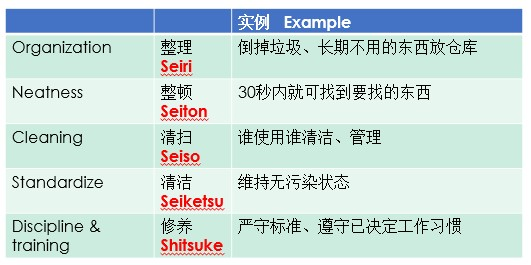
\includegraphics[width=6cm]{5S_五常法_Screenshot_2023-08-03_211606.jpg}\\

\hypertarget{ux53c2ux8003-references}{%
\section{参考 References}\label{ux53c2ux8003-references}}

\begin{enumerate}
\tightlist
\item
  若松义人. 《为什么是丰田:成为第一的方法和7个习惯》
\end{enumerate}





\part{个人提升}自我改善基本功 \\

\chapter{改进从团队开始} % Introduction chapter suppressed from the table of contents

从下面两家美国公司五六十年代做改革的成功故事,让我们了解自主团队如何能带动公司提升。

但是这改进思路并非万事万能,后半部会总结背后的主要成功要素。

\hypertarget{ux7f8eux56fdux8d39ux57ce-weisbord-ux6545ux4e8b}{%
\subsection{美国费城 Weisbord
故事}\label{ux7f8eux56fdux8d39ux57ce-weisbord-ux6545ux4e8b}}

60 年代 复印机还未普及,很昂贵,所以为各类公司客户提供印刷服务就有市场,
这个故事的主人翁是某美国东岸一家印刷公司老板的儿子Weisbord。
他一直都没有接受什么正式的管理培训。 他有一个好朋友 Don
在国际大公司已工作了20 年, Don
推荐Weisbord说:``很多大公司已经开始推进团队自主管理,提升生产率, 
你可以先读 X-Y 理论(McGregor `Human side of Enterprise')一书。''

X 理论:

%\href{文件:0A_Agile_stories_p2.jpg}{文件:0A Agile stories p2.jpg}

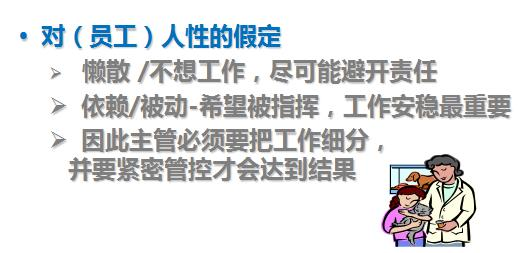
\includegraphics[width=6cm]{0A_Agile_stories_p2.jpg}

Y 理论:

%\href{文件:0A_Agile_stories_p3.jpg}{文件:0A Agile stories p3.jpg}

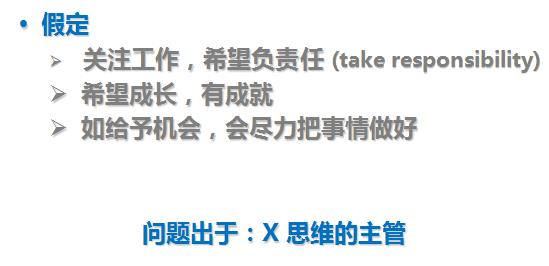
\includegraphics[width=6cm]{0A_Agile_stories_p3.jpg}

Weisbord
本来只想看看有多厉害,但他结果一口气一周末读完全书。他发现自己公司到处都是X
理论管理:

\begin{itemize}
\tightlist
\item
  工作分得很细,每员工不清楚全局
\item
  任务都是依赖主管分配
\item
  员工遇到问题、困难,交给主管处理
\item
  员工上下班打卡
\end{itemize}

他觉得这方式应该可以帮公司提升,但他担心单靠自己推动不了这个改革,
他便请Don过来正式加入公司。\\
他们分析公司业务最大问题是订单处理部门(Order Processing),
每个订单处理工作分到五、六个任务,员工只管被分配的任务,例如:

\begin{itemize}
\tightlist
\item
  筛选客户邮寄地址,邮寄印刷样本
\item
  输入订单
\item
  检查客户的信用
\item
  发起内部生产订单
\item
  用打字机打发票邮寄出去
\item
  收到的支票,对上那些应付账
\end{itemize}

公司平均每天要处理200 到300 个订单,
但因为工作分得很细,如果某个任务(如输入订单)有一、两人缺席,
便严重影响整个流程,效率会降低一半。\\
针对这问题,Weisbord 计划改革,把这部门的人分成多个4-5 人的团队,
把公司的两万个客户按地区分到各团队,每个团队有自己的客户名单,打字机等设备,
希望以此增加部门的灵活度,并提高生产率。\\
Weisbord 与5 位小主管(supervisor)商量,2 位很赞成,2 位中立,其他1
位觉得不会成功。 Weisbord 决策启动这改革,与Don 开始重组部门。\\

\hypertarget{ux5f00ux59cbux56e2ux961fux5236}{%
\subsubsection{开始团队制}\label{ux5f00ux59cbux56e2ux961fux5236}}

开始时问题非常多:

\begin{itemize}
\tightlist
\item
  B 物流公司运送出错,送到另一个城市,怎么办?
\item
  D 团队误解了生产的步骤,怎么办?
\item
  C 团队的样板工人,刚入职3 周,对我们公司产品线不熟识,怎么办?
\end{itemize}

原因很简单:本来每个人以前都只懂自己的一小块工作,以前问题都是由小主管处理。现在自主团队没有主管,都要靠团队自己想办法,像瞎子摸象。\\
但问题确实太多了,没办法,Don 建议每周开会讨论。
他们从未有每周开会的习惯,Weisbord
本来以为开会浪费时间,把时间用于生产更实际。
问题一直都非常多,延续了一个月。\\
Weisbord 开始怀疑这X-Y
理论,只是大学象牙塔里的玩意,难以真正用于实际公司环境。 Don
也没有更好的建议。\\
Weisbord 开始有撤销整个改革的想法,返回本来的组织架构, Don
还希望Weisbord 稍等一两周,看看有没有好转。但Weisbord
觉得一直这么多问题,严重影响公司运作,也难以与父亲交代,想在下次开会时向大家宣布变回本来架构。\\
到了第五周开会:\\
Weisbord,与以前开会一样,先问: 大家有什么问题?\\
沉默,几分钟后,某组长说:没有问题。\\
Weisbord:
为什么会没有?一直这么多问题(心里想,一定是你们也放弃了,连问题都不愿提了。)\\
另一组长回答:我们今周没有什么问题,遇到的问题都在以前的会议里面被解决了。\\

\hypertarget{ux6548ux679c}{%
\subsubsection{效果}\label{ux6548ux679c}}

改革的结果是从原来每天低于300
个订单提升到了400个。员工的出勤率也得到了改善,缺席率降低到接近零。\\
改革后的订单处理部平面图:

%\href{文件:0A_Agile_stories_p5.jpg}{文件:0A Agile stories p5.jpg}

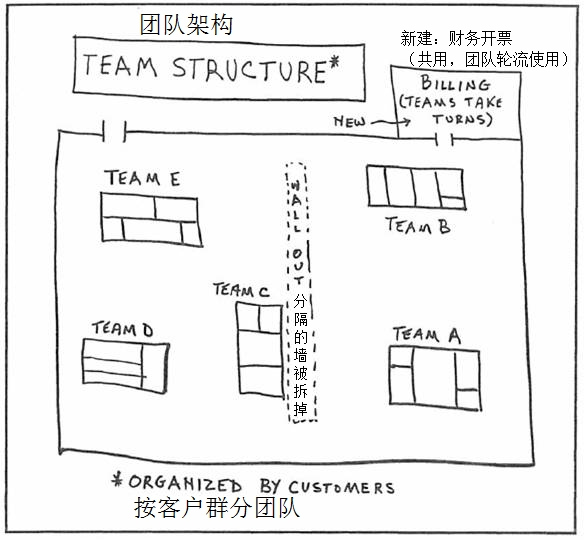
\includegraphics[width=6cm]{0A_Agile_stories_p51.jpg}

(团队自主改革前,小主管们为了减少各功能之间在处理订单引起的争吵,特意在中间加了一道墙;后面团队们一致建议把墙拆掉。)\\
Weisbord 
事后回顾:所有改变,重组都需要时间磨合,过程中管理者的支持非常重要,如果管理者不能坚持,面对并解决面对的困难,便会以失败告终。\\

\hypertarget{weisbord-ux6545ux4e8bux7684ux542fux53d1}{%
\subsection{Weisbord
故事的启发}\label{weisbord-ux6545ux4e8bux7684ux542fux53d1}}

如果员工具备知识技能,管理者便应尽力给员工平台,让团队自主发挥,才能不断提升竞争力,应对变化万千的市场需要,让员工与公司都受益;管理者不仅仅是制定目标、计划,发号施令的角色,而更应该是一位导师,辅助团队成长。\\
::= = = =
Lewin教授(心理学):``必须参与一起分析、讨论,才有动力后面采取行动。We
are likely to modify our own behavior when we participate in problem
analysis and solution, and likely to carry out discussions we have
helped
make.''这些实验也解释了为什么虽然Taylor先生科学管理本应可以提升工人的效率,但因为整个设计都是由专家设计,工人没有参与,所以反对。\\
Lewin 教授的实验与分析启发了随后的学者继续实验研究。

\hypertarget{ux7761ux8863ux5de5ux5382ux5b9eux9a8c-harwood-manufacturing}{%
\subsubsection{睡衣工厂实验 Harwood
Manufacturing}\label{ux7761ux8863ux5de5ux5382ux5b9eux9a8c-harwood-manufacturing}}

二战后,在维京尼亚州(Virginia),Harwood 是一家专门做睡衣的工厂。\\
难题:\\
要按不同的季节需求,做不同款式的睡衣,但往往有些女工习惯了某种工作方式,效率很高,但是要她改变工作方式,就接受不了,很难转换。

实验 - 比较三种变更方式:\\
*按传统方式,依赖工程师去设计每一轮的变更。团队只需要按设计去做。

\begin{itemize}
\tightlist
\item
  每个团队有代表与管理层去讨论如何变更,然后执行。
\item
  自己去策划自己的变更,也提建议。也安排那些女工每周跟那些生产率高和低的女工一起讨论不同方式的优劣,自己讨论怎么改变。
\end{itemize}

实验结果\\
*第一组按传统强制要求她们改变,花了3个月的时间,并引起很多不满,效果也不理想:生产率降低了百分二十,也发现有十个女工里面有一个后面就辞职不做了。

\begin{itemize}
\tightlist
\item
  第二组效果中等,需要大概两周才恢复到本来的水平。
\item
  第三组发现两天后就已经返回本来变更前的生产力水平,后面慢慢的上升提高到百分之十四。例如,某一个实验组就把本来一天45件,五天后提升到87件------一个本来无法想象的数字,后面甚至提到90件,超越本来那些工业工程师的目标。\\
\end{itemize}

这实验验证了集体讨论、自己管理,确实可以提升团队的生产率。结果也验证了实验前的发现:不同工人有自己不同的方式做事,没有像Taylor先生深信那种工作的最佳方式。\\

\hypertarget{ux7ed3ux8bba}{%
\subsubsection{结论}\label{ux7ed3ux8bba}}

问:这些故事是否想表达:我们就好比Taylor先生只是从工程方面去做优化。因为团队人员没有参与分析,导致他们难以接受和执行工程师(我们)设计的最佳方案。

答:你说得对。这些实验验证了群体行为:如果他们有参与或者可以影响结果,他们就有动力去做改进,如果要求他们听专家的最佳方案,往往就没有效果。五六十年代,越来越多公司采纳这个方式去做改进,也很多大学机构做这方面,培训不是用什么传统教学问的方式,而是用一些角色扮演或者团队的集体问题解决,去强调一个团队只要他们有收到及时的反馈,也比较开放,就可以做到一个民主的改进方式。下面另一个实验可以让我们更理解:

\framebox{%
\begin{minipage}[t]{0.97\columnwidth}\raggedright
自己做实验,取数据分析
一家工厂,很多主管都不愿意聘用三十岁以上的女工做机械操作工作,都觉得她们的生产力不如年轻女工高。你估计如果我们做顾问,给他一些数据,它会改变吗?不会。所以顾问只鼓励他们自己去做一些实验,证明那些三十岁的以上的女工确实生产率比年轻的低。他们确实按这个做了各种实验,但分析结果发现那些年纪大的女工无论生产力率,缺勤率、学习速度,更换工作流程的速率,都比年轻的好。后面他们也不再拒绝聘用年纪大的女工了。但其他那些没有参与做实验的团队,一直都不愿意改变。
\strut
\end{minipage}}


\hypertarget{ux7834ux51b0---ux53d8ux9769---ux7a33ux5b9a}{%
\subsection{破冰 - 变革 -
稳定}\label{ux7834ux51b0---ux53d8ux9769---ux7a33ux5b9a}}

以上两案例都可以归纳: 开始团队可以归纳:
自主团队管理都都需要经过下面三个阶段:\\
第一:破冰(Unfreezing),需要提供一些新的信息、新的数据,来减小/降低团队的反对声音。\\
第二:变革(Moving),要他们团队变态度、价值观、架构、行为等等。从以上的实验这个不能仅仅靠一些工程师去设计,最好是让他们自己讨论,得出他们觉得最合适的方式,他们才愿意按他们的讨论去执行。\\
第三:固定稳定下来(Refreezing)。当有了提升以后,需要有一些机制去维护新的行为方式,不要让它退回本来。与团队一起去研究、分析变成行动。顾问只是提供数据去破冰,减小反对的力量。所有变更、变革都会很痛苦、很困难。顾问或者公司管理层都应该有这些心理准备。例如本来的小组长、主管,他要接受在变更后角色的变化,不像以前是像将军一样继续下命令。

也类似过程改进戴明环(PDCA):\\
%\href{文件:IPM.png}{600px}

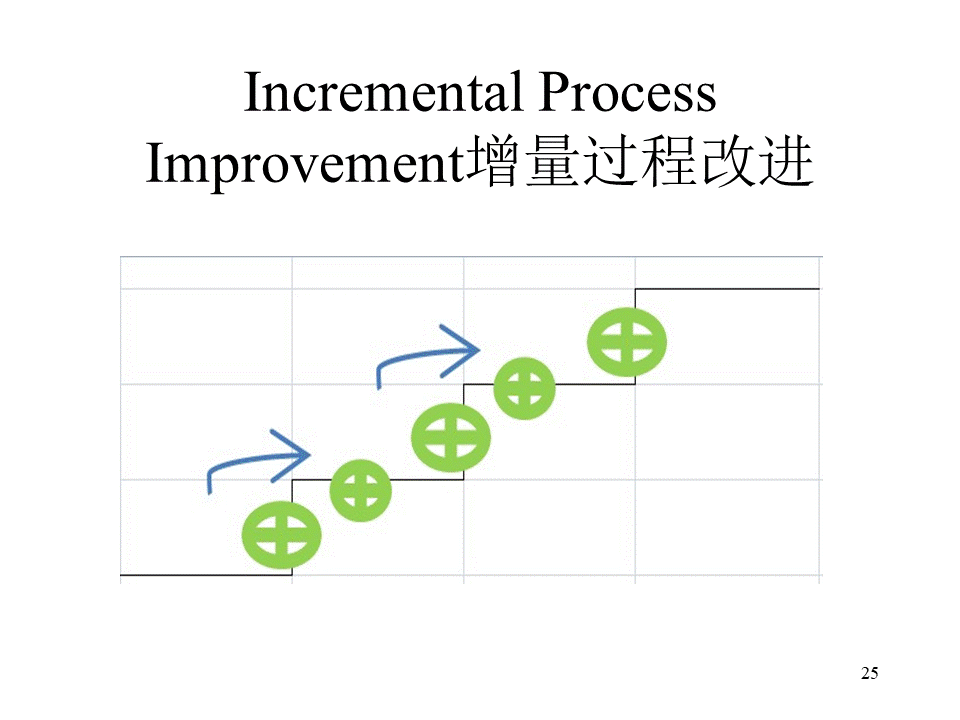
\includegraphics[width=6cm]{IPM.png}

从以上这些实验你应该也可以理解为什么本来Taylor先生那一套科学管理方式的不足。他只是考虑了工作方面、工程方面的因素,忽略了人性方面的考虑。但千万不要忽略工程方面的重要性。

\hypertarget{ux6210ux529fux8981ux7d20}{%
\subsection{成功要素}\label{ux6210ux529fux8981ux7d20}}

上面案例里的Weisbord
先生,后来卖掉了父亲创建的公司,自己成立顾问公司,他从六十年代开始做了几十家美国公司的改革,也发明了六个盒子方法
(Six-Box Model)。他的经验分享:\\
``每次跟企业做访谈、诊断时,一般顾问单是从公司遇到什么问题、什么困难、如何解决?跳出这个圈圈,从更高的角度去想这家公司有什么改进的潜力?有哪些人在公司里面可以持续推进这种改革?有没有一些让公司每个人都愿意参与的改进方向?那现在环境变化很快,顾问的角色应该是跳出为客户解决一些技术问题,诊断给药方,而是挖掘出员工的潜力,让他们动脑筋一起思考如何解决他们遇到的问题,才是一个对企业更有价值的东西。''\\
他建议要注意4个成功要素:

\hypertarget{ux516cux53f8ux6f5cux529b-assess-the-potential-for-action}{%
\subsubsection{公司潜力 Assess the Potential for
Action}\label{ux516cux53f8ux6f5cux529b-assess-the-potential-for-action}}

\textbf{Leadership commitment 领导支持}\\
这点最重要,顾问的责任不是诊断技术问题提供解决方案,更重要是探索公司有没有持续改进的潜力?如果缺乏的话,什么神医也医不了公司的病。

\begin{itemize}
\tightlist
\item
  有没有领导的支持?我接触很多公司,如果高层联系不上,或者不关心质量问题,觉得都可以委托他人解决,就很难做了。最常见就是老板是业务出身,一直都没有太关注软件工程,觉得写一个软件没有什么困难,市场和销售才最重要。反过来,如果有技术总监等,甚至软件工程质量的欠缺或者重要性,兴趣听可能的一些解决方案,这个公司才有潜力做一些持续改进。你可以想象如果我们开展培训,要求他们参加,如果高层不支持,后面什么都做不出来。下面的人也知道我们顾问,或者我们讨论后有什么建议、结果,老板或者高层也不关心,肯定就不会有什么效果。
\end{itemize}

\hypertarget{ux5546ux673a-good-business-opportunity}{%
\subsubsection{商机 Good Business
opportunity}\label{ux5546ux673a-good-business-opportunity}}

公司有没有一些持久的商机。在软件工程竞争很大,如果公司没有一些持久的方案、产品或者针对性。只是靠客户的关系接一些开发项目来做,就很难有一个长期的资源去投入,提升自己的质量。恰恰从我们的经验,这类软件开发公司会越来越难在这个市场上面竞争,比一些有能力、产品化的公司取代。

\hypertarget{ux5458ux5de5ux52a8ux529b-energized-people}{%
\subsubsection{员工动力 Energized
people}\label{ux5458ux5de5ux52a8ux529b-energized-people}}

公司里面有没有一些中层项目经理级别的人愿意投入时间,真心推动改革,原因是顾问只可以短时间帮助公司,长远还是要靠公司内部人员去推动。怎么识别有没有那些人呢?人可以分4种心态:如果是在下面两格的人的话
(Denial=否认 , Confusion=迷惑
),就不用想会支持这种变革,首先必须要是在上面的两格(Contentment=满足 ,
Renewal=更新) 
。所以作为顾问,你要识别有没有这种人,在公司里面要辅助他们作为整个公司改革变化的重要种子。\\
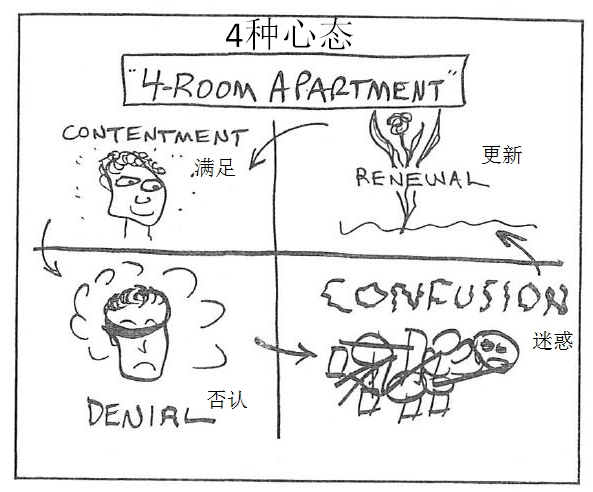
\includegraphics[width=6cm]{P335_4_room_apartment1.jpg}

\textbf{4种心态 与 对策:}

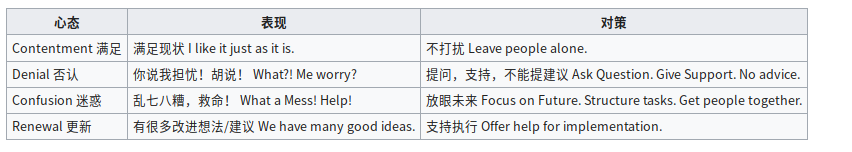
\includegraphics[width=6cm]{Screenshotfrom2023-11-0304-11-55.png}

注意: 人的心态会不断(按环境)循环变化。

\hypertarget{ux6280ux672fux521bux65b0-pocket-innovation}{%
\subsubsection{技术创新 Pocket
Innovation}\label{ux6280ux672fux521bux65b0-pocket-innovation}}

软件工程在技术方面变化很大,从我接触的公司,如果一直都没有使用一些新的技术平台,这类公司可以改进的机会极低。反过来,如果公司在过去做过一些内部的改进,比如引进一些自动化技术,推行持续交付、自动化测试等等,就看到这个公司其实已经在技术方面有很多不断提升、完善的项目在进行中,这个文化就更容易推动所有人参与、改进整个系统的可能性。\\

\hypertarget{ux7ed3ux675fux8bed}{%
\subsection{结束语}\label{ux7ed3ux675fux8bed}}

过程,改进需要每一个部门都参与,才可以提升公司的最终目标,公司是一个系统,所有员工参与改进整个系统:

%\href{文件:微信截图_20231025084623.png}{600px\textbar{}无}

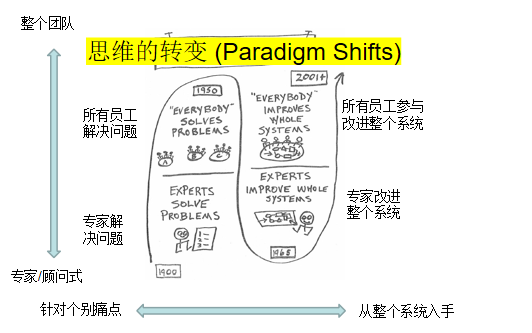
\includegraphics[width=6cm]{微信截图_20231025084623.png}

(上图参考 M. Weisbord, Productive Workplaces Revisited)

如果没有按照上面说的步骤,形成具体行动计划,很难取得效果。

过程改进不是一两个月、两三个月就出成绩,开始时候,员工可以关于创新、改进有想法,写文章分享,但要这个作为习惯继续下去,是需要有些新的想法和思路,这可以借助公司内部培训,比如有没有过程域相关的参考资料、内部分享会、学习小组,定期有老师的辅助指导,定期体检、诊断。


\hypertarget{ux9644ux4ef6}{%
\section{参考 References}\label{ux9644ux4ef6}}

\begin{enumerate}
\tightlist
\item
  McGregor, D.: \emph{The Human Side of Enterprise},1960.\\
\item
  Weisbord, M.R.: \emph{Productive workplaces revisited : dignity,
  meaning, and community in the 21st century}, 2004.
\end{enumerate}





\chapter{克服拖延症} % Introduction chapter suppressed from the table of contents


技术总监问:现在我遇到最大的难题就是如何提升下面技术人员的能力,如果他们全都是高手,我就很轻松了,但实际上高手最多只有三分之一,其他都是中低水平。您接触过这么多软件开发团队,有什么好方案?\\
我:你可以先听听以下故事。\\

\begin{description}
\tightlist
\item[]
= = = = = = = = = =
\end{description}



%\url{文件:超效率目录.png}

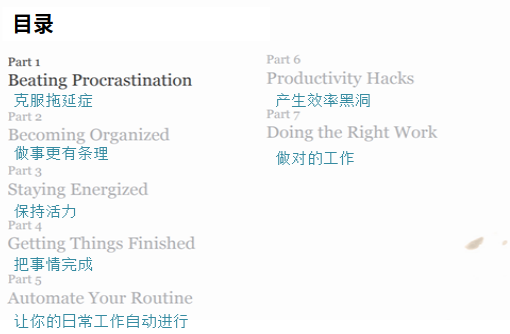
\includegraphics[width=6cm]{Screenshotfrom2023-10-1523-05-00.png}

例如,第一章克服拖延症,这里的内容几乎全部都有帮助:\\



\hypertarget{ux6839ux56e0ux5206ux6790ux8befux89e3ux6848ux4f8b}{%
\subsubsection{周/日目标 (1 Weekly/daily Goals)}\label{ux6839ux56e0ux5206ux6790ux8befux89e3ux6848ux4f8b}}

\framebox{%
\begin{minipage}[t]{0.97\columnwidth}\raggedright
我每天都会定计划,早上希望完成哪些功能,下午完成哪些。当然这个计划也会按实际的进展调整。

周 /
日目标是个人时间管理的基本功。每一天第一件事不是回邮件,而是仔细想想今天要完成什么任务,每一周的开始,也应该想我本周希望完成什么任务。不然的话,每天的时间就很容易被琐碎的小事吃掉,一事无成。\\
\strut
\end{minipage}}

\framebox{%
\begin{minipage}[t]{0.97\columnwidth}\raggedright
背后体现的道理很简单, 要把时间花在重要、但非紧急的活动上,效率才会体现出来。

%\href{文件:紧迫非紧迫_3.0.png}{600px}
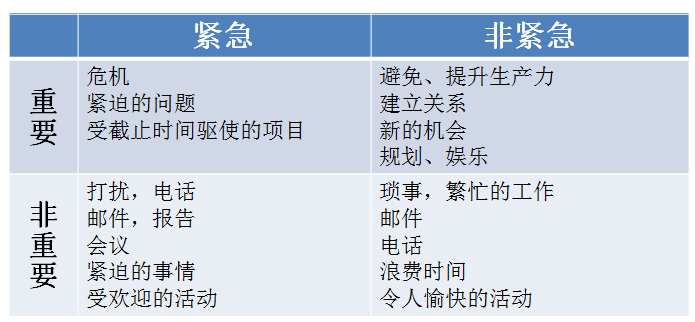
\includegraphics[width=6cm]{紧迫非紧迫30.png}

\strut
\end{minipage}}

\hypertarget{ux6839ux56e0ux5206ux6790ux8befux89e3ux6848ux4f8b}{%
\subsubsection{限定时间 (Timeboxing)}\label{ux6839ux56e0ux5206ux6790ux8befux89e3ux6848ux4f8b}}

\framebox{%
\begin{minipage}[t]{0.97\columnwidth}\raggedright
 把每天的任务安排成时间段,每一段不应超过1.5小时。\\ 
一般人可以专心集中的时间段都不会超过60分钟,小孩可能更短。如果老师叫你星期五5点钟交卷,你不会提前交,都会等到最后十分钟,甚至最后五分钟。所以如果我们把一天的时间切开,分成
1 ~ 1.5 小时时间段,自然有动力,希望在时间之内完成任务。\\
我们写代码的时候应该也是用同样的原理。例如某些编程活动尝试了多次,但没有进展,有时总共会花超过10小时。所以每次当我发现某编程工作超过了2小时,我就会先做其他事情。\strut
\end{minipage}}


\hypertarget{ux6839ux56e0ux5206ux6790ux8befux89e3ux6848ux4f8b}{%
\subsubsection{分解任务 (Dissolving tasks)}\label{ux6839ux56e0ux5206ux6790ux8befux89e3ux6848ux4f8b}}

\framebox{%
\begin{minipage}[t]{0.97\columnwidth}\raggedright
因为都是练习题,所以每一个功能都比较细,不会超过二十行。如果我们平常做开发时,也必须要把一些大、复杂的功能预先拆分成小的功能才有效率。
\strut
\end{minipage}}


\hypertarget{ux6839ux56e0ux5206ux6790ux8befux89e3ux6848ux4f8b}{%
\subsubsection{加强自律 (Building Self-Discipline Muscles)}\label{ux6839ux56e0ux5206ux6790ux8befux89e3ux6848ux4f8b}}


\hypertarget{ux6839ux56e0ux5206ux6790ux8befux89e3ux6848ux4f8b}{%
\subsubsection{晨礼(Morning Rituals) 日常运动 (Make an Exercise Routine)}\label{ux6839ux56e0ux5206ux6790ux8befux89e3ux6848ux4f8b}}


\framebox{%
\begin{minipage}[t]{0.97\columnwidth}\raggedright
不要以为编码是一个单纯的脑力活,整天坐在电脑前面敲代码就可以。如果人的体力、精力没有配合上也会出问题,好在我每天早上一直坚持30
\textasciitilde{}
40分钟的轻量运动,然后晚饭前半个小时到一个小时的骑单车或者慢跑的习惯。中间也是不是整天坐着,一段时间会走一走、喝点儿橙汁等,以确保身体不断在动,这样才不会困,保持动力。

贝多芬每天都会通过去外面散步来获得一些创作的灵感,然后他会立马把这些写在本子上,用于后面的音乐创作。
\strut
\end{minipage}}

我:身体健康,精神状态也同样重要,你每周有锻炼的习惯吗?\\
小李:没有,每天都太忙了,虽然一直觉得身体不如几年前了,也知道锻炼好,但无法抽出时间。\\
我:我也很忙,但深知定期运动对身体非常重要,我一直按以下两方法保持个人身体状态:

\begin{itemize}
\tightlist
\item
  工作时尽量避免长期坐下来,因我主要做培训、咨询、评估,所以可以大部分时间站着或在走动(NEAT\#)。
\item
  尽量每天7点吃早餐前跑圈,疾跑1.5 -
  2分钟,休息半分钟,重复这循环4-6轮(HIIT\#)。
\end{itemize}

\hypertarget{ux6839ux56e0ux5206ux6790ux8befux89e3ux6848ux4f8b}{%
\subsubsection{不会分心的工作场所 (Create a Distraction-Free workplace)}\label{ux6839ux56e0ux5206ux6790ux8befux89e3ux6848ux4f8b}}

\hypertarget{ux6839ux56e0ux5206ux6790ux8befux89e3ux6848ux4f8b}{%
\subsubsection{轻策划、迭代、再策划 (Ready , Fire, Aim!)}\label{ux6839ux56e0ux5206ux6790ux8befux89e3ux6848ux4f8b}}

\framebox{%
\begin{minipage}[t]{0.97\columnwidth}\raggedright
三十年前,软件开发都是一些大型的项目,整个架构要设计好才动手去写代码。现在反过来,需求变化极大,开发都需要敏捷,轻文档、轻计划,尽尽快写好代码,做一些功能给客户,从反馈优化下一轮。我这次的几天开发也是用同样原则,没有花时间在一些设计或者文档。想直接把代码写出来,并通过单元测试,节省了很多耗时间的工作。把有限的时间都放在写好代码上。
\strut
\end{minipage}}


\hypertarget{ux6839ux56e0ux5206ux6790ux8befux89e3ux6848ux4f8b}{%
\subsubsection{不断清洗 (Churning)}\label{ux6839ux56e0ux5206ux6790ux8befux89e3ux6848ux4f8b}}

\framebox{%
\begin{minipage}[t]{0.97\columnwidth}\raggedright
万事开头难。我在开始的半天也是遇到同样问题,不知如何入手,太久没看写代码的书了,很多基本的都不知如何入手。所以我开始的时候不会直接尝试写题目里面的功能,而是重写一些书本的代码,看看跑出来怎么样,然后逐步提升。写一些基本功能,慢慢有了习惯,调整过来了,后面就越来越顺。好比一台旧的水泵,刚开始抽上来的水总是有难喝的铁锈,只要不停止抽水,当污水最终都从系统中抽出后,就能发现底下的净水。
\strut
\end{minipage}}

\hypertarget{ux6839ux56e0ux5206ux6790ux8befux89e3ux6848ux4f8b}{%
\subsubsection{要有好的土壤 (Remove your Hidden Roadblocks)}\label{ux6839ux56e0ux5206ux6790ux8befux89e3ux6848ux4f8b}}

\framebox{%
\begin{minipage}[t]{0.97\columnwidth}\raggedright
在含盐量高的土壤里种植物是结不出果实的。浇水、平衡在阴凉处和阳光下的时间都抵不过根部吸入的毒素。如果我们没有积极性,就可能是土壤的问题。如果没有足够的积极动力,就不会在长假专注写程序,也不会定期要求自己写分享文章。所以要有明确、很想达到的目标驱动。
像一个作曲家,他希望写出很多经典的优秀作品,不满足于现在的状态。觉得自己的灵感或者创造力没有发挥出来,成为可以保留下来的东西。也是这种驱动力让我可以一直努力做这件事。
\strut
\end{minipage}}


\hypertarget{ux6839ux56e0ux5206ux6790ux8befux89e3ux6848ux4f8b}{%
\subsubsection{摒弃拖延恶习 (Quit your Procrastination Vices)}\label{ux6839ux56e0ux5206ux6790ux8befux89e3ux6848ux4f8b}}

\framebox{%
\begin{minipage}[t]{0.97\columnwidth}\raggedright
长假里,大部分人都会把时间用于看视频或电视剧,而我正好没有这个习惯,也一直没有玩网络游戏的习惯,否则肯定完成不了。
\strut
\end{minipage}}

最终我用日程记录(Timelogging),把整件事和什么活动、时间花在什么地方都记录下来了。

小李:我看你上面列出的技巧,我大部分都还没做到。

我:不要紧,我六年前刚开始定期写文章时跟你一样,但只要不放弃,一直往既定目标努力,不良习惯都改正过来了。我常常说人的潜力是极大的。舒伯特你听过吗?\\
小李:好像是一个很有名的作曲家。\\
我:是的,但他31岁就去世了,你猜他一生一共写了多少首歌和音乐作品。\\
小李:我记得中学时,老师介绍过他的艺术作品,如《鳟鱼》,但他31岁就死了,我猜100 \textasciitilde{} 200 首歌?\\
我:他一生写了超过460首歌曲(时长\textgreater{}24小时)。除了歌曲,他还写了其他作品,如9首交响曲(1首未完成,1首只有草稿),20
室内乐,120 钢琴曲等,每一类都包括大量经典作品,对后世影响深远。\\
小李:如果粗算一下,他一生约有600作品,算他有16年时间作曲,平均每月要完成3个作品,真是不得了。\\
我:虽然他的作品有大有小(从一首歌到45分钟的交响曲),他确实生产率极高,而且他最后的7年身体一直都不好,所以他那个时候肯定不会像我们现代996方式工作。
他每天主要是早上用来写作,傍晚便去休息散步。但他会同时做多个创作项目。
如果项目没有灵感,就暂时放下来,创作其他作品。
他著名的未完成交响曲就是个好例子,只有两个乐章(一般交响曲都是四个乐章)
所以他是使用高效技巧的一个成功例子。
每个人都有自己的理想,但如果没有高效率来执行,理想只是天马行空,天方夜谭,不会有任何成就。
除了以上这些技巧外,保持整洁也重要。你有没有试过想找某东西,找半天都找不着?

小李:确实经常发生,而且还会遗漏东西。我上次出差便忘记了iPhone,后面回北京后电话联系当地酒店前台后,我找当地同事去酒店取,然后快递给我,烦死了。\\
我:有听过5S (5S法\#)
吗?例如,如果你把东西都放固定地方,就可以避免同类问题再发生。如果你一直在一个很乱的环境工作,回导致心情烦躁,对工作、身体都不好。

\begin{description}
\item[]
\begin{description}
\tightlist
\item[]
(\#详见附件”锻炼之道”的多了解  NEAT, HIIT;5S法详见第1章附件。)
\end{description}
\end{description}

小李:我大概懂你的意思了,要提升自我能力先要改变习惯,有了良好习惯(如时间管理),才可能提升。\\

\begin{description}
\tightlist
\item[]
= = = = = = = =
\end{description}

总监:我大概懂你的意思了,要提升技术人员的能力先要改变他们的习惯,有良好的习惯(如时间管理),才有机会提升。\\

\framebox{%
\begin{minipage}[t]{0.97\columnwidth}\raggedright
即时笔记 (The Capture Device)
总监边听边在本子上记下那些重点。高效的人都会有工具帮他记录想到的灵感、想法、项目、待做事项等,不会仅仅靠大脑记忆。你提出一个要求,他会立马写在小本子上,你会觉得他应该会按你要求去处理,但反过来如他只是口头说会处理,你会担心很可能没有下文。但我看有些领导,身边只拿个手机,除非他们的记忆力超人,否则我估计他每天都会忘记不少重要事项。
\strut
\end{minipage}}

\hypertarget{ux7ed3ux675fux8bed}{%
\subsection{结束语}\label{ux7ed3ux675fux8bed}}

\framebox{%
\begin{minipage}[t]{0.97\columnwidth}\raggedright
杭州某高级经理的高见
人一定要自律!您说的小技巧确实能起到很大帮助,而且我基本都会使用,但如果不养成习惯,想起来使用下,最终还是改不了拖延症,所以要解决拖延症,一定从根源做起,还是得靠自己,需要培养自己意志力、专注力,坚持好习惯,改掉坏毛病。
\strut
\end{minipage}}

我相信人分高低,但并非取决于基因、种族,主要取决于她后天的习惯、自律与努力。要养成良好习惯要从小开始,深受家庭和教育的影响,所以百年树人。

与公司改进一样,改变个人习惯很难,这些技巧可以帮助个人改善。

\hypertarget{ux9644ux4ef6}{%
\section{附件}\label{ux9644ux4ef6}}


\hypertarget{ux953bux70bcux4e4bux9053-the-truth-about-exercise}{%
\subsection{锻炼之道 The Truth about
EXERCISE}\label{ux953bux70bcux4e4bux9053-the-truth-about-exercise}}

想大家都同意和相信:
``多运动,便多烧耗卡路里,便能帮助减肥,降低体重。''

\framebox{%
\begin{minipage}[t]{0.97\columnwidth}\raggedright
某国家给市民的健康指南:每周起码做150分钟中强度锻炼,或75分钟高强度锻炼。
\strut
\end{minipage}}


但不是每个人都能每天抽时间做锻炼,有什么更好方法?\\
不一定只依赖去健身室锻炼,平常工作生活少坐多走,站着工作、开会,甚至小动作等都有帮助。

\framebox{%
\begin{minipage}[t]{0.97\columnwidth}\raggedright
N.E.A.T. (Non-exercise activity thermogenesis) 小实验;
教授使用有电子传感器的底裤,记录记者、咖啡厅女服务员、商务人员三人一周每天正常工作中消耗多少卡路里。\\
发现:

\begin{itemize}
\tightlist
\item
  女服务员最好。因每天都非常忙碌(尤其是早餐时段),送餐、接单、做咖啡等等。
\item
  商务人员第二。虽然有很多时间坐下来,但每天都会走一公里路见客户,而且每周二、五下班后会去健身锻炼。
\item
  记者最差。每天无论工作或家里,大部分时间都是坐下不动,所以他看起来不胖,但其实体内存有大量脂肪,集中在肝、肾等内脏。
\end{itemize}\strut
\end{minipage}}

这实验告诉我们:如果每天一直坐下不动很不好,就算每天下班后晚上都去健身锻炼也帮不了。

后面记者听教授建议,改变习惯,定期站起来走动。如与同事交流与尽量边走路边交流,减少长期坐下来;
多爬楼梯,少用电梯;骑单车,不开车等方式。
后面,从实验数据分析,发现这些改变帮他增加每天卡路里消耗接近一倍,到500水平。

研究发现不断大量健身锻炼不一定对每个人都有效。
有20\%会没有效果,另一端对15\%的人会非常有效。
这跟人的基因密切相关,所以多锻炼不一定都有效。

\begin{description}
\tightlist
\item[]
= = = = = = = = =
\end{description}

实验发现,如锻炼能快速提升心跳率到最高,然后休息,反复做 4 - 6轮,
效果不会比大量健身锻炼差。
例如,每天做几轮40秒的冲刺,把心跳速度快速提升到极限,
效果可以比长时间的缓步长跑更好。

\framebox{%
\begin{minipage}[t]{0.97\columnwidth}\raggedright
HIIT (High Intensity Interval Training) 小实验;
教授与助手教记者使用运动单车做 HIIT:
用尽全力练20秒,休息,再同样做两轮;每周三次。

记者按教授要求完成了四周HIIT锻炼,虽然帮他提高了血液分解糖份的能力,减少糖尿病风险;
但提升不了他的最高带氧运动量。教授解释这是因记者的遗传基因是属于没有效果的20\%。
\strut
\end{minipage}}

\hypertarget{ux53c2ux8003-references}{%
\section{参考 References}\label{ux53c2ux8003-references}}

1. YOUNG, Scott: "The Little book of Productivity" 《超效率手册》\\


%1011

\part{自我管理开发过程}软件开发工程师自我改进过程\\

\chapter{三点估算} % Introduction chapter suppressed from the table of contents

\hypertarget{ux4f30ux7b97ux662fux4e00ux4e2aux8303ux56f4ux4e0dux662fux4e00ux4e2aux6570}{%
\subsection{估算是一个范围,不是一个数}\label{ux4f30ux7b97ux662fux4e00ux4e2aux8303ux56f4ux4e0dux662fux4e00ux4e2aux6570}}

唐工:你估计要完成开发用户登录模块要多少天?\\
小李:三天。\\
唐工:能在三天完成的可能性有多高?\\
小李:可能性很高。\\
唐工:可否量化一点?\\
小李:可能性为50\%-60\%。\\
唐工:所以很有可能不止三天,要四天了。\\
小李:对的,其实也有可能要五、六天,但我估计机会不大。\\
唐工:你信心有多少?\\
小李:难说,有95\%的信心可以在六天之内完成。\\
唐工:所以有可能要用上七天了?\\
小李:这样说吧,如果所有可能出问题的都出了问题,甚至会10天或11天,但这种概率很低。\\
(最终管理者唐工还是要求有一个承诺,而不是一个估算)\\
所以唐工再问小李:是能否给我一个确实能完成这个模块的日期?\\
小李:正如我前面说,很可能三天可以完成,但有可能四天。\\
唐工追问:你可以说四天吗?\\
小李:也有可能五六天。\\
唐工结束对话:OK,请你尽力六天之内完成这个模块。\\
唐工貌似请求,但实际是要求小李承诺这个模块要在六天之内开发完。假如这个模块的开发时间超过六天,唐工就有依据说小李没有尽力导致延误了。\\
所以从以上对话,可以看到作为开发专业人员,必须分清估算和承诺。作为专业人士,我们不应该给一些没有把握的承诺,误导对方。中国老话说一诺千金就是这个道理。

\hypertarget{ux4eceux5355ux70b9ux5230ux4e09ux70b9ux4f30ux7b97}{%
\subsection{从单点到三点估算}\label{ux4eceux5355ux70b9ux5230ux4e09ux70b9ux4f30ux7b97}}

从上面的例子可以看到,一般的单点估算是很容易被误导,以为那个天数是有把握达成的,所以我们最好从单点估算变成三点估算,除了估算最可能的天数,还有最佳和最差共三点。但项目是由一系列的任务组成(如第二任务依赖于第一个任务的完成),如何计算所有任务的总天数?
下面用例子说明如何用3种使用3点估算估计的方法(A、B、C)估算总天数:\\
A)假定都是正态分布,用模型估计:\\
先用PERT方程式计算每一步的预计值 与 标准差:\\
::预计值 Expected Value EV = (Best + 4xMost Likely + Worst ) /6\\
::标准差 Sigma= (Worst - Best) / 6\\

%Screenshotfrom2023-11-1221-23-06.png

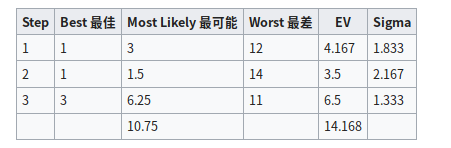
\includegraphics[width=6cm]{Screenshotfrom2023-11-1221-23-06.png}

如果假定是正态分布,按以上预计值和标准差,使用蒙特卡洛模拟,从下图可看到,95\%范围是
8.02 \textasciitilde{} 20.37\\
%\url{文件:pert3.1.png}

\includegraphics[width=6cm]{pert31.png}

B) 直接用PERT方程式计算总天数的均值与标准差:\\
如不用模拟,直接把3步的均值加起来\\
::4.2 + 3.5 + 3.6 = 14\\
计算3步总方差:(方差 = \(Sigma^2\))\\
假定: 总方差 = 每步方差的总和\\
总方差 = 9.77\\
Sigma \(\sigma\)= 3.13\\
95\%范围计算公式为:均值的总和
\(\pm 2 \sigma = (4.2 + 3.5 + 3.6) \pm 2 x 3.13  = 14 \pm 6.26\)= 7.74
\textasciitilde{} 20.26\\
结果与蒙特卡洛模拟预测类似。\\
C) 假定都是三角形分布,用模型估计:\\
如果用三角形分布,95\%范围是 10.38 \textasciitilde{} 26.45\\
%\url{文件:pert32.png}

\includegraphics[width=6cm]{pert32.png}

\hypertarget{ux603bux7ed3-ux89e3ux8bfbux5206ux6790ux7ed3ux679c}{%
\subsection{总结 +
解读分析结果}\label{ux603bux7ed3-ux89e3ux8bfbux5206ux6790ux7ed3ux679c}}

\begin{itemize}
\tightlist
\item
  如果假定每一步的分布都是一个正态分布,就可以用头两个方程式计算每一步的平均值跟标准差和方差,用方程式可计算3步的总均值大概是14。也可以用方程式计算标准差,总的sigma
  (标准差)是3.13左右。
\item
  也可用蒙特卡洛模型(假定步骤都是正态分布),得出很类似的正态分布,总的平均也接近14,95\%的范围是从8.02到20.37,
  接近上面算出的均值 \(\pm\) 两个标准差数值。
\item
  但因三个步骤都是明显往右偏,所以不能假设它们是正态分布,更合适的是使用三角形分布,然后用蒙特卡洛估算``加''起来的分布,看见最后一个图明显是类似往右有个尾巴,能更正确反应三个步骤加起来的天数的估计分布。
\item
  跟假定正态分布的结果比较,很明显看到用三角形分布结果往右偏,上限是
  26.45(比正态分布的20.37
  高)。不是正态分布的话,左面就没有长尾巴,所以就会比本来正态分布的下限高,下限是
  10.38 (比正态分布的 8 高)。
\item
  从这简单例子看到,如果我们要把三点估算加起来,尤其是非正态分布的话,就不能用简单的方程式,或者假定它是正态分布来计算,需要用蒙特卡洛模型假设三角形分布才能真正反应总体的分布。\\
\end{itemize}

从这三个偏左分布步骤例子看起来好像有些偏差,但不是很严重。如果我们看见用十个步骤都是偏一边分布,总分布会如何?是否相差会更远?

\hypertarget{ux5229ux7528ux8499ux7279ux5361ux6d1bux6a21ux62df10ux4e2aux6b65ux9aa4ux4e09ux89d2ux5f62ux5206ux5e03ux7684ux603bux5206ux5e03}{%
\subsection{利用蒙特卡洛模拟10个步骤(三角形分布)的总分布}\label{ux5229ux7528ux8499ux7279ux5361ux6d1bux6a21ux62df10ux4e2aux6b65ux9aa4ux4e09ux89d2ux5f62ux5206ux5e03ux7684ux603bux5206ux5e03}}

如果每步都估算天数,10个步骤的 总天数就是500天 (把10个估算值加起来)。

但如果每个步骤都是三点估算:

%Screenshotfrom2023-11-1221-25-44.png

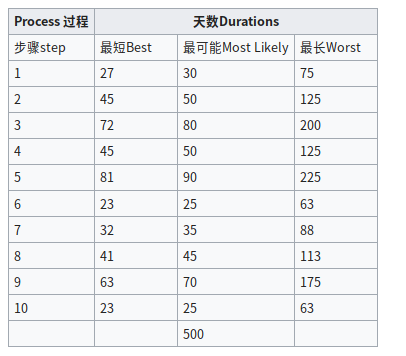
\includegraphics[width=6cm]{Screenshotfrom2023-11-1403-10-17.png}

很明显看到每一步都是偏左的分布,所以可预计总天数应不止500天,
但估多少才合适?

假定每步骤是三角形分布,用模型估计,重复五千次,得出下面分布:

%\href{文件:HMTT_v1.3_s77.png}{400px}

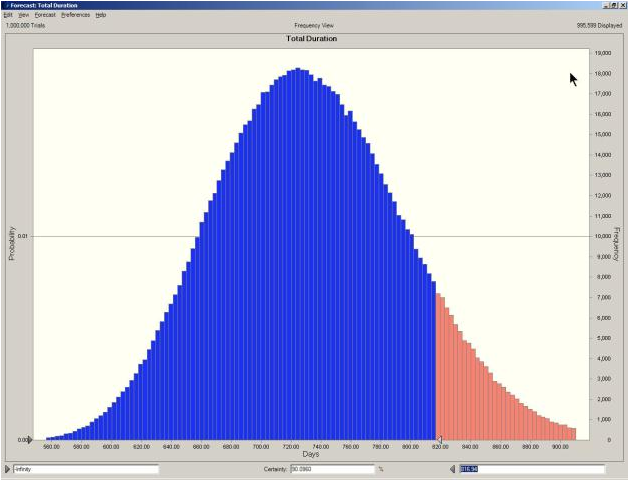
\includegraphics[width=6cm]{HMTT_v13_s77.png}

%Screenshotfrom2023-11-1221-27-17.png

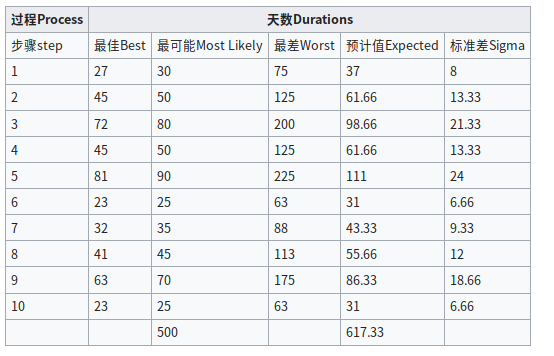
\includegraphics[width=6cm]{Screenshotfrom2023-11-1403-10-57.png}

A) 用PERT方程式计算每一步的预计值 与 标准差:

%\href{文件:10stepsPertScreenshot_2022-10-24_205007.jpg}{500px}

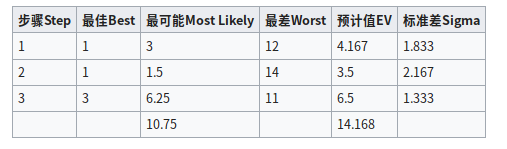
\includegraphics[width=6cm]{Screenshotfrom2023-11-1403-12-52.png}

假定是正态分布,按以上预计值和标准差,使用蒙特卡洛模拟,得出的总分布与上面用三角形分布的结果几乎一致,都是左右平均分布的正态形。

\hypertarget{ux5206ux679010ux6b65ux9aa4ux6a21ux62dfux7ed3ux679c}{%
\subsection{分析10步骤模拟结果}\label{ux5206ux679010ux6b65ux9aa4ux6a21ux62dfux7ed3ux679c}}

\begin{itemize}
\tightlist
\item
  为什么用三角形模拟出来不是偏左的分布(类似前面3步结果),而是一个正态分布
\end{itemize}

\begin{description}
\tightlist
\item[]
以上实验验证了``中心极限定理'',无论本来是什么形状的分布,如果随机抽样够多,样本的平均值分布接近正态分布。所以如果本来只是3个步骤的时候还是可以看出是三角形偏左,但到了用十个步骤相加的时候,就跟每个都是用正态分布去估算的结果没有什么区分。\\

(中心极限定理会在后面数据分析里用上,例如通过画控制图判断过程是否稳定)\\
\end{description}

\begin{itemize}
\tightlist
\item
  实验结果也验证了PERT三点估算法公式,无论任何分布都可以用PERT公式计算每一步的预计值和标准差,然后计算总结果的分布(不需要蒙特卡洛模拟),当步骤越多差异就越小,如果是像上面的例子,只是希望求10个步骤的总分布(无论每步本身是怎样分布),都不需要用模拟,用PERT公式计算便可。\\
\end{itemize}

\begin{description}
\tightlist
\item[]
(这不表示蒙特卡洛模型没有用,到后面根因分析部分,我们还是会继续用它来比较不同的搭配选择最优)
\end{description}

\hypertarget{ux9644ux4ef6}{%
\section{附件}\label{ux9644ux4ef6}}

\hypertarget{ux8499ux7279ux5361ux6d1bmonte-carlo-ux6a21ux62df}{%
\subsection{蒙特卡洛(Monte Carlo)
模拟}\label{ux8499ux7279ux5361ux6d1bmonte-carlo-ux6a21ux62df}}

当结果不能用数学公式计算的时候(例如是三角形分布),可以用电脑随机模拟结果。例如:

\begin{itemize}
\tightlist
\item
  计算3个步骤的总共人天,每个步骤都是三角形分布,我们就用电脑的随机功能模拟,让随机功能的结果按三角形分布:
\item
  第一次模拟:步骤1得出1.3,步骤2得出1.2,步骤3得出2.0,得出三个步骤的总工期是4.5人天。
\item
  第二次......。
\item
  如果我们模拟1000次,10000次就有,便能模拟出总分布。
\end{itemize}

5000次

%\href{文件:捕获2-1.PNG}{500px}

%\href{文件:捕获2.PNG}{500px}

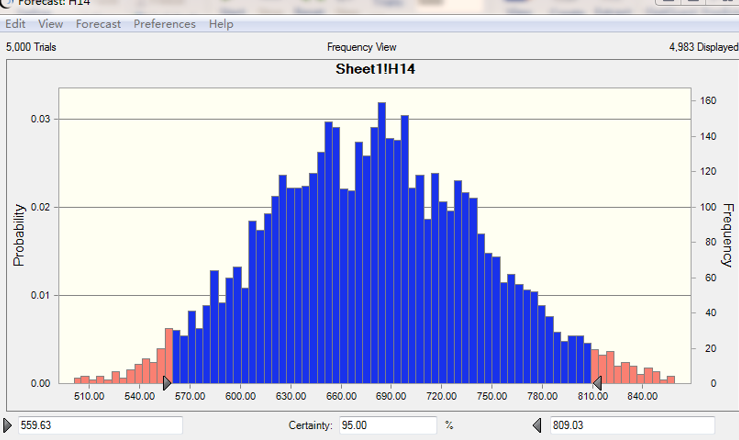
\includegraphics[width=6cm]{捕获2-1.PNG}

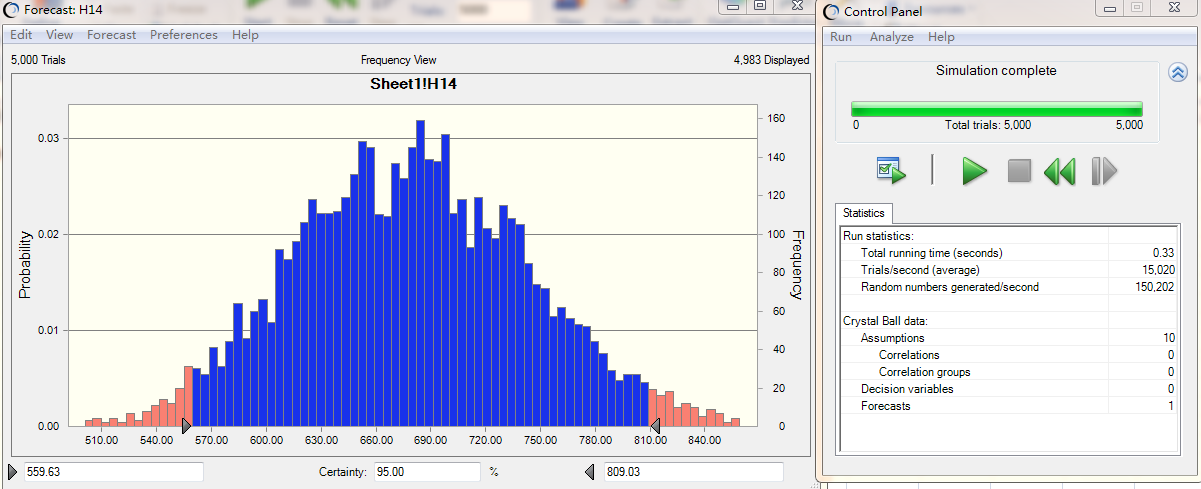
\includegraphics[width=6cm]{捕获2.PNG}

10000次

%\href{文件:捕获1-1.PNG}{500px}

%\href{文件:捕获1.PNG}{500px}

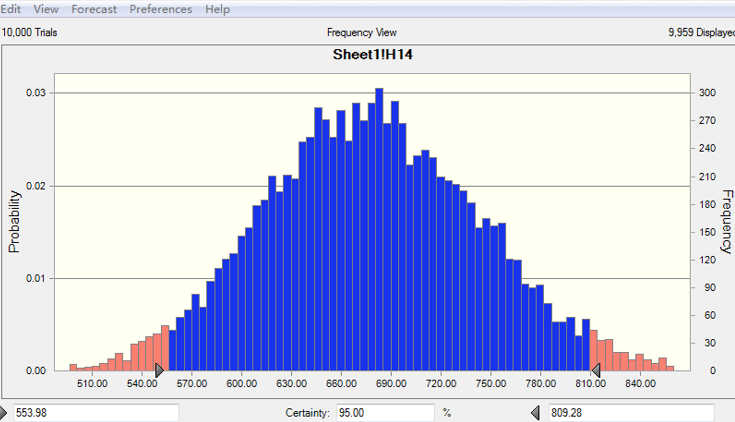
\includegraphics[width=6cm]{捕获1-1.PNG}

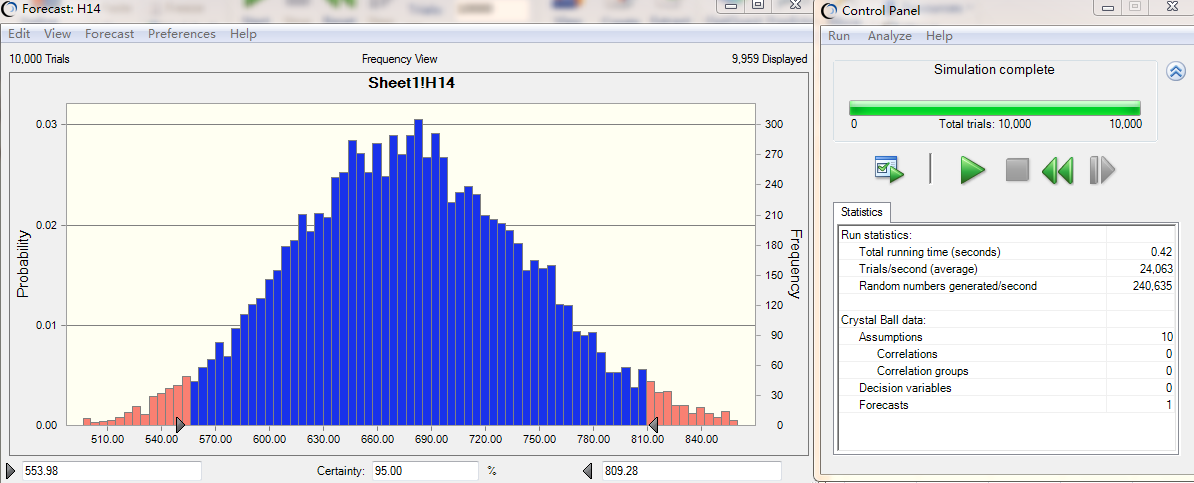
\includegraphics[width=6cm]{捕获1.PNG}




\chapter{量化管理从个人开始} % Introduction chapter suppressed from the table of contents

\framebox{%
\begin{minipage}[t]{0.97\columnwidth}\raggedright
我:你们管理层和客户都比较关心项目的进度,项目是否能按时完成?请问你们过去的项目如何?\\
开发:我们现在就是走敏捷开发,两周一个迭代。每次迭代前,我们聚一起开会,把所有用户故事按优先级排序,估计这个迭代可以完成哪些任务?然后放在看板的待办事项里。每天我们会做站立会议,监控实际的进展。\\
我:你们都能按计划在冲刺迭代里把所有任务开发好吗?\\
开发想了一下,说:我们也有延误出现,有些模块不能在计划的冲刺里完成。\\
我:为什么?\\
开发:我们花了很多时间修正系统测试暴露的问题,有一些是因为前面没有把需求分析透导致的返工。\\
我:请问你们是怎么估计每个任务应该花多少时间?\\
开发:我们会一起讨论,然后用敏捷的扑克牌方式,集思广益来估计。\\
我:除了你们每天站立会议监控项目的进展,你们要不要统计一下项目延期的水平是多少?\\
开发:其实我们也不算是延误,有些模块不能在本迭代完成,就放在下一个迭代去做。\\
我:软件开发有一个系数叫每人的生产率,就是开发人员一天能产出多少有效代码?你们有统计吗?\\
开发:你说的是否是敏捷开发燃烧图里的速度?我们有画,但发现变化波动很大,所以后面我们也没有再用。
\strut
\end{minipage}}


\hypertarget{ux5982ux4f55ux964dux4f4eux9879ux76eeux8fdbux5ea6ux504fux5dee}{%
\subsection{如何降低项目进度偏差}\label{ux5982ux4f55ux964dux4f4eux9879ux76eeux8fdbux5ea6ux504fux5dee}}

从以上对话可以看到,敏捷开发不一定能帮助团队按期交付,开发人员也不清楚自己的生产率是多少。要减少项目的延误,首先取决于估算是否准确。但如果只是依赖个人经验、头脑风暴去估计,很可能低估,因为可能没有考虑开发以外的一些因素,比如缺陷问题、需求问题等。在同一个冲刺里,不能交付所有计划的模块,等同于延误。要做好估算,就需要有数据。数据需要从个人收集的历史数据作为参考。IT公司是否有注意这方面?我们可以从他们的新员工入职培训探索一下。

\framebox{%
\begin{minipage}[t]{0.97\columnwidth}\raggedright
我:请问你们如何培训新入职的开发人员?\\
培训师:我们会先上一些基础的理论课,培训公司的代码规范、框架和复用的模块。然后进行个人或小组练习,我们会简化一些简单的开发项目里面的某个模块,让他们照着做个小项目,然后我们就会对他们的成果进行反馈,让他们知道自己的开发水平如何,是否掌握了我们所培训的内容。\\
我:他们会收到什么反馈?\\
培训师(想了一下):依据他们是否掌握了培训内容的重点来打分。\\
我:怎样打分?\\
培训师:我们依据评判标准打分,分数从1到5,1最低,5最高。\\
我:评判的标准可以说说吗?\\
培训师:(想了一下)
依据他们是否掌握了培训内容的重点打分。\\
我:你们公司不是已经开始推行量化项目管理,是否应该也配合量化管理,不仅仅靠老师主观判断来打分?\\
培训师:可否举些例子?\\
我:例如他们质量方面的缺陷数,如果他们有做单元测试或者评审相关阶段的缺陷排除,项目管理相关所花费的工时,从而可以反算出编码的效率等客观的量化指标。
\strut
\end{minipage}}

\hypertarget{ux4eceux91cfux5316ux57f9ux8badux5f00ux59cb}{%
\subsection{从量化培训开始}\label{ux4eceux91cfux5316ux57f9ux8badux5f00ux59cb}}

从以上对话可以看出很多公司都没有与量化软件开发项目管理相关的培训,这样如何能希望他们在项目中做好量化管理?入职不仅需要培训开发的技巧、怎么写好程序、做好面向对象设计,也应该学到要一直度量自己的开发过程,包括所花的工时、过程中发现的缺陷数等。\\
培训师会问:在新员工培训时,如何可以加入这些量化的元素呢?\\
很简单。首先,在先培训质量相关的技术指标,比如什么叫质量成本、什么叫排除率等,然后做实战练习时,要求他们除了写程序,还需要记录一下所花的工时,自己项目检查时发现的缺陷数、测试的缺陷数、评审所花的时间等。也要求开发人员除了提交程序以外,提交一个开发计划报告,内容包括实际所花工时、本来预估的工时、过程里发现的缺陷数、在哪一类过程等。帮助他们一进入公司就培养一些量化度量的习惯,以避免过了试用期,开发的习惯已经养成,后面是很难改变的。

\hypertarget{ux4eceux4f30ux7b97ux7b56ux5212ux5230ux76d1ux63a7}{%
\subsection{从估算、策划到监控}\label{ux4eceux4f30ux7b97ux7b56ux5212ux5230ux76d1ux63a7}}

挣值分析(Earned Value,EV)是常用的项目监控技巧,如果简单用百分比监控项目的进度或工作量偏差,因缺乏明确定义,难以比较,挣值分析把计划、实际等都统一用成本来计算,没有项目管理工具也可以简单手工计算(EV公式与示例,详见附件)。Humphrey先生出版了不少书,他也用EV分析来监控进度,他在PSP书中以此为实例,介绍如何用挣值分析策划与监控。我也试用挣值法来监控写这本书的进度(详见附件案例)。下图是PSP估算与监控的流程:

%\href{文件:PSP_fig7.2.jpg}{350px}

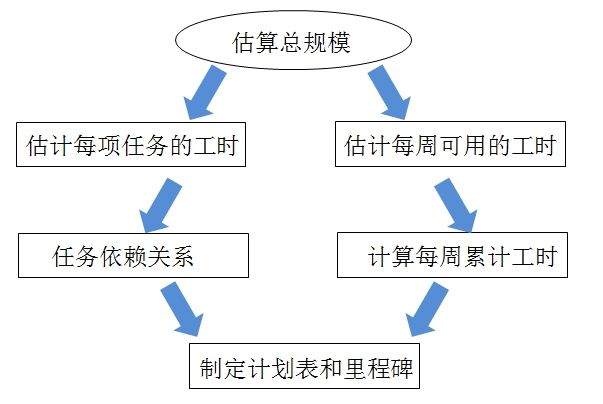
\includegraphics[width=6cm]{PSP_fig72-1.jpg}

可以把敏捷的燃烧图方法看成挣值分析法的简化版,挣值分析也可以按现在的速度来预计完成的时间(燃烧图假定每一轮迭代的速度不变)。\\
传统大型项目每个时间段投入的工作量会有变化,挣值分析法可以按当前的进展和投入预计完成时的总成本。\\
想了解如何使用高中低三点估算和PERT方程式估算总工作量与范围,详见附件里的案例。\\

%挣值分析不仅仅用于监控软件开发项目,先生在他书中举例说明他如何用来监控他写书的进度。我也用同样思路来监控本书的进度(详见附件)。\\
%传统大型项目每个时间段,投入元素、工作量都会有变化,挣值分析法可以按当前的进展和投入预计完成的情况。但无论是挣值分析法或者燃烧图都是单点估算。\\
%从附件的案例里面看到,如果难以估算任务单点值,可使用高中低三点估算,然后利用PERT方程式估算总工作量与范围。\\

%\hypertarget{ux603bux7ed3}{%
%\subsection{总结}\label{ux603bux7ed3}}

很多软件开发项目延误的原因是以前没有收集历史数据,导致估计所需人时都很理想。我也有同样问题:从我的挣值分析实例看到,因我是第一次写书,之前也没有养成统计章节所花的实际工时的习惯,所以在11月初做估算时,理想地认为最多花一个月完成,但过了3周就发现,实际比本来计划延误很多,原因包括:

\begin{itemize}
\tightlist
\item
  实际可用工时没有想象这么理想,有很多意外事情都要处理。
\item
  低估了完成一章节所需时间:

  \begin{itemize}
  \tightlist
  \item
    例如第一个章节TDD实际所花的工时与估计差不多,原因是这个章节是现有的,只是做了一些调整,所花时间不多。
  \item
    但到第二个章节MGR就不一样了,全部内容都重新写;如何从实际客户现场的场景总结,与理论结合也很花心思。
  \end{itemize}
\end{itemize}

所以下次当你遇到一些团队项目延误,可以问项目经理以下问题:

\begin{enumerate}
\tightlist
\item
  如何估算项目工期\\
\item
  如何估算每一项任务所需的工时,依据是什么?\\
\item
  如何收集实际工作量?\\
\item
  如何监控累计到现在的完成情况?\\
\item
  有没有统计以往的历史数据?如何用来帮助做好估算?\\
\end{enumerate}

你可能会发现类似我用挣值分析估算和监控暴露出的问题。

\hypertarget{ux5e94ux8be5ux5982ux4f55ux6539ux5584}{%
\subsection{应如何改善}\label{ux5e94ux8be5ux5982ux4f55ux6539ux5584}}

软件开发和工业生产不同,工作量数据必须靠个人自己收集,量化管理依赖个人习惯,所以Humphrey先生在90年代推出了PSP个体软件过程,教导开发人员如何一步步自己收集数据、自己估算、自己监控。例如记录花了多少工时、发现多少缺陷、完成多少代码(从最基础开始,逐步改善),尽量减少缺陷返工,提升开发效率。(详见附件PSP简介。)

也正因为大部分的团队都没有收集数据的良好习惯,没有PSP的基础,所以就很难要求他们在冲刺回顾时拿出数据,分析根因、在下一轮迭代改善,从定性提升到量化管理。当开发人员养成好习惯,就会更清楚知道自己的速度和质量水平,不会出现本章开头的场景,开发人员对自己的质量水平或生产率一无所知。

有些企业深知量化管理对企业发展很重要,所以在新员工培训时,不仅仅教他们技术技能,也教他开始自己每天记录工时、缺陷数等习惯。
因为工作习惯养成后,便难以改变。反之,如果周边的人都有记录数据,自己也觉得应做记录,逐渐形成公司文化。

\framebox{%
\begin{minipage}[t]{0.97\columnwidth}\raggedright
\textbf{问答Q\&A}\\
\textbf{资深敏捷顾问}:我大约20年前对这个东西比较熟,PSP 包含2个重点:

\begin{enumerate}
\tightlist
\item
  关于个体的估算内容,这个我看您的文章里边表达得比较充分。
\item
  关于缺陷记录分类统计和根因分析的内容,这一块实际上相当于是CMMI里需要个体配合的地方。我看您几乎没有提到。
\end{enumerate}

我:非常赞同,若要做到本手册后面提到基于缺陷数据的量化根因分析并改进,就要依赖个人记录缺陷与返工工作量,碍于篇幅有限,这里先用人时的估算与监控带出PSP的思路。\\
顾问:我自己也是在某军工航空项目里边用过一次。我们当年计划少、跟踪多,大家本来就缺少生产率的概念,所以其实也不知道每天能干什么事,但只要记下每天干了什么事,然后比对这个基数做就可以了,无论快或慢,都需要看看到底是什么原因。

我:您觉得这种方法有用吗?\\
顾问:因为开发依赖人的创造力,写新程序其实很难准确估计所需时间,但我后来发现如果估算是由组长负责去做,就能起很大的作用。例如有一次,我看有一个程序员花了一个月时间用Java写了某模块,接近1万行代码。虽然我不熟悉Java语言,但觉得代码有点问题。后面我就找另外一个比较资深的组长,我们3个人一起看代码。评审并删除无用的代码,最后剩下不到100行代码就可以实现了。如果当初我们先做好这模块的估计,就可以避免一个月人时的浪费。所以我建议还是需要估算,但是应该由有经验的技术组长负责。

我:很好,你很熟悉敏捷,例如SCRUM里用扑克牌方法估算,你觉得怎么样?\\
顾问:我先跟你讲个故事。我曾参加某冲刺估算会议,他们用扑克牌方法估算“数据显示” 故事点,其中一位估计是8,另外一位估计是40。为什么会差这么多呢?第一位解释只需要展示数据,确实该工作量不大。但第二位理解就不一样了,包括整个数据的分析、输入和展示等,整个过程工作量确实很大。从这里可以看出,如果没有统一理解需求,就难以估算。所以那次以后,需求分析应分成“实体”和“行为”,清晰地写出功能需求,减少误会。(这是功能点估算规模的概念。)

我:赞同。Humphrey先生在PSP书里强调,要参考历史数据来做好估算,其实也可适用于敏捷估算。不应靠人的主观判断。\\
顾问:是的,所以我前面强调必须要由经验的主管去负责估算。估算很重要,但是要程序员自己去估很难。所以PSP20年前的思路,还能适用于现在的敏捷开发团队,帮助他们做好估算。\\
PSP里强调要评审设计、代码并分析缺陷,当时因为只靠人手,所以会很耗时。现在,我们有类似SONAR的静态扫描工具,可以像机器人一样,做本来耗时的代码评审工作。但SONAR只能针对一些基本语句问题,针对整个OO设计,我们会建议用我们的工具去扫描,补充SONAR扫描的不足。跟PSP代码评审的思路一样,所有扫描出的问题都必须修正。有些团队觉得问题太多了,只处理掉那些重大的问题,剩下一些可能不会直接影响到功能的问题暂时不处理。我不赞同这思路,这么多的问题其实都是累积出来的,如果从一开始都一直有定期处理清空,就不应该累积大量问题,而且这些问题遗漏下来还是对程序有隐患。\\
我:很赞同,
归根到底还是开发人员缺乏保证质量的意识。最近有个团队也是用工具扫描代码,然后我问他为什么找出的部分问题不处理。他说例如定义某个变量,但是没有用,虽然被扫出是问题,觉得不影响程序的运行就不处理。我解释说,这样就好像放了一个地雷,后面还是会爆炸的,所以还是应该要处理。
\strut
\end{minipage}}

PSP 要求评审代码,分析每个发现的缺陷,讨论原因,然后改进。有些管理者听过PSP,但认为PSP成本太高,只适用于高价值、高质量要求的项目。如果他们理解PSP能最终帮团队把缺陷返工减半,能降低开发成本20%,便不会再觉得PSP不适用于公司。(后面会有相关例子。)\\

估算很重要,要做好,不仅仅要参考历史数据, 也需要对需求有共同的理解。\\
功能点方法是估算软件规模的一种标准,下一章会用实例介绍。

\hypertarget{ux9644ux4ef6}{%
\section{附件}\label{ux9644ux4ef6}}

\hypertarget{ux6323ux503cux5206ux6790ux6cd5earned-value}{%
\subsection{挣值分析法(Earned
Value)}\label{ux6323ux503cux5206ux6790ux6cd5earned-value}}

用最简单的例子,来说明挣值分析中PV、EV、与AC的意义。

\begin{description}
\tightlist
\item[]
PV:计划完成多少?
\item[]
AC:完成工作的实际成本是多少?
\item[]
EV:实际完成了多少工作?
\end{description}

公式:

\begin{description}
\tightlist
\item[]
进度偏差 SV = EV - PV , SPI = EV / PV 完成占计划完成的百分比
\item[]
成本偏差 CV = EV - AC , CPI = EV / AC 完成的价值占实际已花成本的百分比
\end{description}

本文实例主要关心进度偏差,所以没有计算 AC

以下面“使用挣值分析监控案例”为例:

截止到22.11.20 , PV 累加本应是 27.5,EV 只有 3.1

\begin{description}
\tightlist
\item[]
所以 进度偏差 SV = EV - PV = 3.1 - 27.5 = -24.4 工时
\item[]
            SPI = 3.1 / 27.5 = 11.27\%
\end{description}


用PERT公式估算头三周任务累积工时的95\%区间(工时):\\
不用MonteCarlo模拟,直接把12(=1+4+7)章节任务 的ExpectedValue 加起来\\
计算12步总方差:(方差 = \(\sigma^2\))\\
总方差 = 每步方差的总和\\
总方差=1.69( \(\sigma\)= 总方差的平方(Sq.Root))

\begin{description}
\item[]
\begin{description}
\tightlist
\item[]
EXCEL 公式为:SQRT(SUM(所有方差范围)) = SQRT(SUM(H3:H15))\\
\end{description}
\end{description}

\begin{description}
\tightlist
\item[]
95\%范围下限(=55.8)

\begin{description}
\tightlist
\item[]
EXCEL 公式为:SUM(所有Expected范围)-2×总方差 = SUM(F3:F15)-2×I15
\end{description}

95\%范围上限(=62.5)

\begin{description}
\tightlist
\item[]
EXCEL 公式为: SUM(所有Expected范围)+2×总方差 = SUM(F3:F15)+2×I15
\end{description}
\end{description}

%\href{文件:PSPcalculate3wks95rangeScreenshot_2022-11-26_105325.png}{500px}

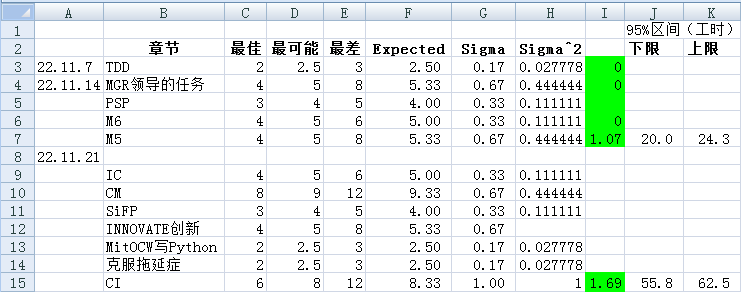
\includegraphics[width=6cm]{PSPcalculate3wks95rangeScreenshot_2022-11-26_105325.png}

\hypertarget{tipsux5982ux4f55ux7b80ux5355ux8bb0ux5f55ux5de5ux65f6}{%
\subsection{如何简单记录工时}\label{tipsux5982ux4f55ux7b80ux5355ux8bb0ux5f55ux5de5ux65f6}}

如前面``克服拖延症''里提到,每人根据自己的习惯,采用每日ToDoList的方式,然后在开始前,简单记一下时间,结束时也记下时间。然后每日/每周统计每任务总工时:

%\href{文件:Psp手工时间表12.jpg}{550px}

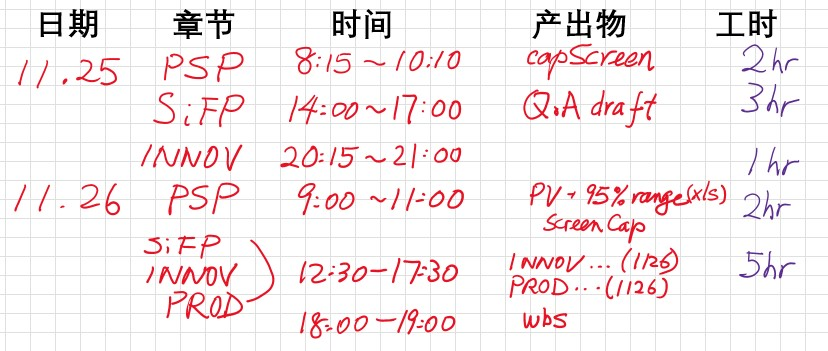
\includegraphics[width=6cm]{Psp手工时间表121.jpg}

如只是个人,不一定需要项目管理工具;如果是团队,可把自己手工记录上传到项目管理工具,方便团队记录与监控。

\hypertarget{ux4e2aux4f53ux8f6fux4ef6ux8fc7ux7a0b-personal-software-processpsp-ux7b80ux4ecb}{%
\subsection{个体软件过程 Personal Software Process(PSP)
简介}\label{ux4e2aux4f53ux8f6fux4ef6ux8fc7ux7a0b-personal-software-processpsp-ux7b80ux4ecb}}

\framebox{%
\begin{minipage}[t]{0.97\columnwidth}\raggedright
PSP 的简单介绍\\

\begin{itemize}
\tightlist
\item
  \textbf{PSP0} 基础 - 工时:计划与实际对比; 每阶段引入多少缺陷 ;
  排除了多少缺陷
\item
  \textbf{PSP0.1} 加入代码行统计 - 计划与实际对比 ; 代码规范
\item
  \textbf{PSP1} 加入使用 PROBE 方法 做规模估算
\item
  \textbf{PSP2} 加入设计与代码评审的计划与统计
\item
  \textbf{PSP3} Cyclic process 先做策划与总体设计,然后多轮开发 ,
  有点类似迭代开发。
\end{itemize}\strut
\end{minipage}}

PSP跟CMMI成熟度模型类似,也是按部就班一步步,帮助软件工程师利用度量改进自我的开发过程。

\hypertarget{psp-0.1}{%
\subsubsection{PSP 0.1}\label{psp-0.1}}

第一步PSP先估计写某个模块所需要的时间和实际花的时间,记录所有的缺陷,包括因为需求、设计或者实现引起的问题,记录修复时间,从开始发现问题直到缺陷被解决,提升到PSP0.1策划不仅仅是估计所需时间,加入了规模的概念,本来PSP是用代码行数来估计规模,也可以使用简化功能点方式估计规模大小。\\
在PSP0.1的阶段还没有用规模做策划、估算,只是记录实际的规模,里面包括基本规模,就是在开发之前软件系统本来有多大。也记录删除、改变、增加、复用的规模数等。最后总的规模数应该是等于基本、新增、删除、复用相加。

\hypertarget{psp1}{%
\subsubsection{PSP1}\label{psp1}}

下一步,PSP1就有规模计划的概念,跟依据0.1的规模定义一样,我们在做开发之前,先估计刚才的所有规模数,并用回归方程估算对应的工作量或者进度,包括偏差的范围。\\
在
PSP0.1增加了一个过程改进建议的环节,依据上一次迭代的数据,发掘下一轮可以完善的改进过程。也加入了编码标准,这个跟我们前面章节提到代码规范的概念相同。所以在PSP0.1,除了计划,也需要有一个叫过程改进经验教训的部分,每一轮都应该有复盘回顾的概念,来提升个人个人的开发过程。

\hypertarget{psp1.1}{%
\subsubsection{PSP1.1}\label{psp1.1}}

PSP1.1基于的PSP1的基础,加入挣值分析法去监控实际的项目进展,加入了PV和累加的PV,计划多少和EV挣值和累计的挣值,反应实际完成多少。从那些系数也可以算出一个叫CPI成本性能指数,来反应完成与计划怎么比较,是否有延误,预计什么时候可以完成。详细可以看用挣值分析法估计写书完成时间的实例。

\hypertarget{psp2}{%
\subsubsection{PSP2}\label{psp2}}

到PSP2就开始增加评审的概念,包括设计评审、代码评审。这些同行评审是很有效的方式,避免缺陷等到出事才暴露、出现问题,因为如果只依赖测试暴露缺陷的话,只是告诉你这个程序跑不通,你还是要看代码才知道问题在哪里,怎么修正?但评审就直接看代码,首先它可以让很多缺陷在评审就发现,不用等到测试才暴露问题。评审也可以找出一些不一定测得出来的问题,例如有些银行对系统质量要求很高,核心的算法不能有任何错误,他们都会要求核心模块必须走专家评审,因为他们也知道很多核心算法的问题不能单靠测试来发现和处理。
也是这个原因,很多公司也会要求代码必须走静态扫描,利用扫描机器人评审代码,预先发现一些明显代码违规的语句问题,弥补单靠人手去评审的不足。\\
有了基础,再加入缺陷密度的概念,即缺陷数除以模块的规模大小,本来PSP是使用代码行的,我们也可以用功能点取代代码行,因为单看缺陷数无法比较,无论个人或者整个团队或者团队之间,所以必须除以规模大小,才可以把系数归一,变成一个项目组之间,人之间可以比较的系数。也引入了排除率的概念,如果我们只是做了评审,但是都是0发现,你的缺陷排除率就是零了,一点效果都没有,所以排除率可以看成是当前评审发现的缺陷数除以当前系统内总共引入的缺陷数,比率越高越好。也有阶段或者过程的排除率,就是这个阶段开始时总共有多少缺陷,然后在这个阶段里我们找出多少,作为分子的一个比例。还有一个就是缺陷排除的速度,按每小时评审的时间找出多少缺陷来判断评审中,可以找出缺陷的速度有多快,评审的效率有多高。

评审质量是PSP2.1 的概念,2.1
也增加质量成本(COQ)概念,与前面敏捷回顾篇里强调软件开发缺陷越后发现,返工量越会以几何式上升的思路一致。

\hypertarget{psp3}{%
\subsubsection{PSP3}\label{psp3}}

接近敏捷迭代的思路,把程序分成不超过几百行的模块,然后把模块按优先级分到不同的迭代
,但还需要有需求与设计。敏捷增加了精益的思路,因为需求可能会有变,所以可以暂时不做后面迭代的估算,只先针对当前的迭代去做策划、估算。
敏捷里面的迭代回顾跟PSP的回顾如出一辙。\\
大家可以参考PSP书里面的教材和练习,比如在书中要求学员自己编写程序,自己记录时间。虽然现在开发语言统计方法跟90年代有差异,但原理还是共通的。如果对新员工难以安排学校式的一周课程,也可以考虑用自学的形式,按要求去记录学习、写报告。

\framebox{%
\begin{minipage}[t]{0.97\columnwidth}\raggedright
学PSP,培养好习惯
所以编程人员可以用PSP的原则,要他们记录。因为现在是写程序,不是玩游戏,所以更贴近实际。也要求后面的程序,让他分析自己的返工成本、质量成本、缺陷排除等,让后面项目团队回顾时有真实数据做分析。

例如在新员工培训时,练习中要求他们有编码规范的概念,按照公司的规范参考来写程序,在每一次做开发之前,都先简单计划一下时间和预估缺陷数。开发完后,记录实际的时间与缺陷数,因为虽然不仅仅是写一个程序,下一次开发时,可以参考以往练习的数据来更好估计,会看到自己的估计越来越准。
\strut
\end{minipage}}

\hypertarget{ux4f7fux7528pspux6323ux503cux5206ux6790ux76d1ux63a7ux6848ux4f8b}{%
\subsection{使用挣值分析监控案例}\label{ux4f7fux7528pspux6323ux503cux5206ux6790ux76d1ux63a7ux6848ux4f8b}}

今天11月8日,离年底要交付全部初稿的时间不到2个月,书的内容也完成了超过一半,但剩下的时间因为年底密密麻麻很多评估,而且评估就是早上9点开始到下午5、6点结束,只有中间一些空档时间和周末可以自由安排,所以我就用同样的思路来策划估算是否能在年底完成要求。
第一步算出现在到年底可以用在写书的时间,按每周估计:

%\url{文件:psp3.jpg}

\includegraphics[width=6cm]{psp3.jpg}

第二步从历史的数据估算剩下的章节,每个章节需要多少小时,写出计划的完成顺序,然后依据原计划可以使用的时间,按最佳使用算出每个章节可以在哪周完成,写在表格的右面空白处,从而估算何时可以完成所有章节,如果确实不能在12月底完成,就可能要重新调整、策划,是否有一些章节优先级比较低,暂时不放在第一版。

因觉得单点估算很难定一个点数,便用三点估算法。每一行估计都有三点:最差、最佳、最可能,用
PERT方程式估计预计(Expected) 和 标准差(Sigma)。\\
挣值分析法所有东西 --
EV、PV、AC都是用钱来结算(这个例子我们就是用所花工时),例如我们估计了每个章节所需要的工时,利用三点估算计算出每个章节预计的工时,加起来得出预计总工时是80.33工时(用PERT公式计算)。例如第一个章节TDD,预期工时是2.5,除以80.33就得出0.031,我们就用3.1作为TDD的PV(所有任务完成的总PV大概是100)。同样方式算出MGR章节的PV是6.6。得出每一个章节对应的PV后,我们就可以计算累计的PV数:

%\href{文件:psp1.1.jpg}{600px}

\includegraphics[width=6cm]{psp11.jpg}

估计哪一周可以完成哪些章节,得出总体的进度计划。例如第三周累积有66工时,应可完成总共12(=1+4+7)
个章节,因用PERT 三点估算,累积工时95\%范围是(55.8 \textasciitilde{}
62.5)。

%\href{文件:PSP3wksPlanScreenshot_2022-11-26_085813.jpg}{600px}

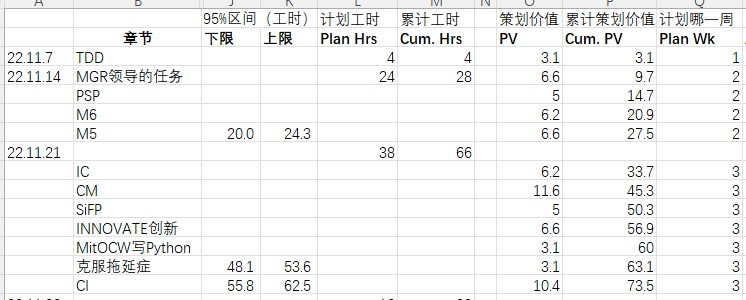
\includegraphics[width=6cm]{PSP3wksPlanScreenshot_2022-11-26_085813.jpg}

\hypertarget{ux76d1ux63a7}{%
\subsubsection{监控}\label{ux76d1ux63a7}}

按实际完成的情况就可以填EV挣值,挣值的算法很简单,必须整个章节完成才算有挣值,不接受部分完成。比如第一周虽然TDD章节已完成九成,但实际是到第二周开始才完成,所以第一周的挣值为0。到了第二周才把本来的第一章节完成,所以里面才放上它的PV(=3.1)。监控的好处,好比要准备半年后的马拉松,开始长距离慢跑(LSD)锻炼,再进一步做连续马拉松配速训练,每周3天,每次5-15公里,速度是多少?比如平均每公里花费6.25分钟。有了数字才知道现状与标准的差距,才有动力对自己说现在离比赛不到12周,必须加强锻炼才能赶上。\\
要让项目有更大的机会按期完成,便需要监控,这样可以预计自己离最后交付差距多少,如果按现在的进展要到哪一周才可以完成,都可以从数字预计出来。但是我们写书也靠灵感,跟写程序类似,可能顺序不一定能按本来的执行,怎么办?\\
其实道理也一样,你可以按新的顺序更新一下本来的计划,把实际的填上。如果你是用简单的Excel表,这个改变可能只花几分钟,很快就能调整好顺序。例如现在看到的第二章节,本来计划放在后面才写,但因刚好与客户接触后产生了灵感,便放在前面写了。

%\href{文件:PSPend2ndWkEvScreenshot_2022-11-26_091326.jpg}{600px}

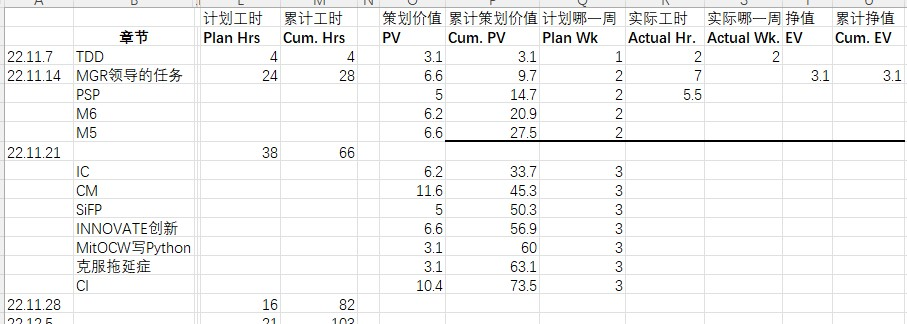
\includegraphics[width=6cm]{PSPend2ndWkEvScreenshot_2022-11-26_091326.jpg}

要估算任务工时便要依赖以往类似活动的历史记录,如果不是每天记录,过后无法记住。每周依据个人的习惯,每天记录实际所花小时数,然后统计每周累计数。\\

\hypertarget{ux53c2ux8003references}{%
\section{参考References}\label{ux53c2ux8003references}}

1.Humphrey, Watts S. ''A Discipline for Software Engineering.''\\
2.Humphrey, Watts S. ''PSP: A Self-Improvement Process for Software Engineers.'' \\



\chapter{估算软件规模} % Introduction chapter suppressed from the table of contents

\hypertarget{ux4e3aux4ec0ux4e48ux8981ux4f30ux89c4ux6a21}{%
\subsection{为什么要估规模}\label{ux4e3aux4ec0ux4e48ux8981ux4f30ux89c4ux6a21}}

规模可以帮我们:

\begin{enumerate}
\tightlist
\item
  依据历史数据策划,例如估算工作量、工期
\item
  归一(Normalize)不同项目,作比较
\item
  知道现在水平
\end{enumerate}

依据历史数据策划先把项目分成组件,参考以往类似的组件所花工作量,估算整个项目的总工作量。规模大小可简单看成是组件的数量。如果是新开发,以前从未做过同类开发,就只能靠个人经验直接估算工作量或工期,但是如果以前做过类似的工作,就可以参考以前的历史数据估算。

规模可以帮我们把不同项目归一。例如,验收测试缺陷数无法比较,但缺陷率(缺陷数/规模)便可以比较;生产率(规模/所花总工时)便可比。

有了归一后可比较的系数,个人/团队便更清楚当前的水平(质量或生产率)是否在上升或下降。

\hypertarget{ux4e3aux4ec0ux4e48ux4e0dux5e94ux7528ux4ee3ux7801ux884cux6570loc}{%
\subsection{为什么不应用代码行数(LOC)}\label{ux4e3aux4ec0ux4e48ux4e0dux5e94ux7528ux4ee3ux7801ux884cux6570loc}}

在1996年前,IBM一直使用代码行数估算规模。之前一直都使用近似机器语言的Assembly
Lang,但为了提升效率,引入了高层语言
PL/S,发现不能再用代码行数来估算规模因PL/S 只需要更少代码行数
也能完成同样功能:

%Screenshotfrom2023-11-1301-59-06.png

\includegraphics[width=6cm]{Screenshotfrom2023-11-1301-59-06.png}

上表是IBM(1968 - 1975)对两种编译器的统计:\\
每个月
PL/S产出代码行数(400)反比Assembly(583)少,但是如果用功能点数便能真正反映生产率的提升:\\
PL/S:8.00对比Assembly:3.33

\hypertarget{ux53eaux9002ux7528ux4e8eux7f16ux7801}{%
\subsubsection{只适用于编码}\label{ux53eaux9002ux7528ux4e8eux7f16ux7801}}

下表中,代码行数只能反应编程的工作量,但编码仅占项目总工作量的一部分,如果把项目按工作量分成以下五个部分,代码行数只能用于第二部分编码(25\%),其他4部分(30\%
+ 20\% + 15\% +10\%)都不合适。

\includegraphics[width=6cm]{Screenshotfrom2023-11-1302-00-20.png}

\hypertarget{ux4e0eux529fux80fdux70b9ux6bd4ux8f83}{%
\subsubsection{与功能点比较}\label{ux4e0eux529fux80fdux70b9ux6bd4ux8f83}}

能估算好项目规模可帮助我们更好估算工作量,规模应具备以下条件:

\begin{enumerate}
\tightlist
\item
  要和工作量密切相关
\item
  要容易数得出来
\item
  容易在项目早期可以估算到
\end{enumerate}

功能点比较符合以上条件,只要功能需求明确,就可以估算出对应的功能点数。

只要需求明确便可以准确客观的估算功能点数。因功能点估算已经是国际标准,基于功能点的度量数据可以与其他国家的标杆对比。

\hypertarget{ux600eux6837ux4f30sifp}{%
\subsection{怎样估SiFP}\label{ux600eux6837ux4f30sifp}}

有了功能性需求,并识别出系统范围,就可以开始估算功能点。

\begin{enumerate}
\tightlist
\item
  数据功能(简称实体)的数量 × 7 (实体是系统要管理的数据)
\item
  业务功能(简称行为)的数量 × 4.6 (行为可以简单看成是增删改查等功能)
\end{enumerate}

\begin{description}
\tightlist
\item[]
简化功能点数=上面1和2的总数
\end{description}

例如,附件例子一潜水学校新开发项目:

\begin{itemize}
\tightlist
\item
  识别出3个实体和24个行为,得出简化功能点数131.4 = 3 × 7 + 24 × 4.6
\end{itemize}

潜水学校二次开发项目:有些功能删除,有些功能变更,就需要分开计算动态功能点和静态功能点:

\begin{itemize}
\tightlist
\item
  静态功能点可以看成是整个系统的功能点数,所以变更的功能点数不会引起影响,但删除的话就需要减去。
\item
  动态功能点主要是用于估算本期开发项目的工作量,因为无论变更功能或者删除功能,都会导致有开发工作量,所以不能是零或负数。国际功能点的规定很简单,都加起来。
\end{itemize}

所以这次二次开发的动态功能点是:

\begin{description}
\item[]
\begin{description}
\tightlist
\item[]
2 × 7 + 11 × 4.6 (增加两个实体和十一个行为)
\end{description}

+ 1 × 7 + 3 × 4.6 (变更一个实体和三个行为)

+ 0 × 7 + 2 × 4.6 (删除两个行为)

= 64.6 + 20.8 + 9.2
\end{description}

再加上 4.6 (因为有数据转换,所以需要加一个CFP,等于4.6)\\
最终动态功能点是99.2 (= 64.6 + 20.8 + 9.2 + 4.6)

静态功能点: 新开发 , 加上新增, 减去删除的功能点

\begin{description}
\item[]
\begin{description}
\tightlist
\item[]
= 131.4 + 64.6 - 9.2

= 186.6
\end{description}
\end{description}

\hypertarget{ux4eceux6545ux4e8bux70b9ux8f6cux7b80ux5316ux529fux80fdux70b9}{%
\subsection{从故事点转简化功能点}\label{ux4eceux6545ux4e8bux70b9ux8f6cux7b80ux5316ux529fux80fdux70b9}}

因故事点只是每个团队自己定义,无法用来作为组织级标准衡量规模,所以很多公司(尤其是银行)转用功能点来衡量软件开发规模。它不仅可用于公司内,也适用于行业标杆,功能点也适用于公司内或公司间结算,例如软件维护期开发工作量变化很大,也难以事前预估,所以有些银行会按最终开发出来的功能点数结算使用部门付开发部的费用,减少争议。

虽然功能点分析源自70年代,但由于计算较复杂,一直未普及,有些人觉得IFPUG
FPA太复杂。针对这问题,国际功能点协会简化本来的功能点算法,推出简化功能点(SiFP),减少了估算的工作量与学习难度(例如培训可以从以往的2天半降到半天)。因简化功能点不考虑实体/行为的复杂度,它与本来功能点的估算有\(\pm\)
15\% \textasciitilde{} 20\% 偏差(详见附件子)。
因敏捷团队是按每轮迭代估算(而不是一次性估整个项目),偏差就可以接受(例如2周一个迭代,偏差大概1.5天),所以SiFP能适用于敏捷多次迭代估算。所以越来越多团队开始从故事点转简化功能点,但由于不熟识功能点估算是从用户角度估算,而非从开发工程师的视角,团队初次估算SiFP通常有误。下面是某成都团队从故事点转简化功能点的案例:

\framebox{%
\begin{minipage}[t]{0.97\columnwidth}\raggedright
客户:我们以前一直使用故事点,为了更好做量化管理,我们新的项目开始使用简化功能点SiFP。\\
我:好的,看一下你的估算表,为什么这两个功能要分成两个行为?\\
客户:这两个功能都挺复杂,估计需要很多开发工作量。我们以前用故事点估算时,也会分成两个故事点。\\
我:请注意,在功能点估算是否是一个行为,取决于它算不算是一个基本过程。如果俩行为互相依赖,不能单独作为基本过程,就不应该分开为2个功能点。很多团队刚开始用功能点,与你们一样,没有弄清楚基本过程的概念,还是从工程师的角度,估计开发时间的工作量来判断是一个功能还是两个功能?在故事点用这种方式估算习惯,但因为功能点是要同一个功能上需求,不能有功能点数的差异,所以不能用估计开发难易程度来判断。\\
客户:可否举个实例?\\
我:以网约车为例,是否可以分成以下9个``行为''?

%\href{文件:sifp_p50图.jpg}{600px}

\includegraphics[width=6cm]{sifp_p50图.jpg}

\begin{enumerate}
\tightlist
\item
  预约申请
\item
  接收预约
\item
  检查是否有可用的车/司机
\item
  寻找其他可选
\item
  提供预约信息
\item
  处理预约
\item
  分派司机
\item
  接乘客
\item
  完成预约请求
\end{enumerate}

客户:是的,每个行为都要花一定开发工作量。\\
我:其实按SiFP只有4个行为,因开头5个和最后2个都要合并才可以成行为(详见附件)。
如果要能独立成行为,必须符合基本过程条件。
基本过程不是随便定的,它有规则,比如从网约车案例我们可以看到,``预约申请''本身不能算一个基本过程,虽然预约申请可能要很复杂的开发工作,但是因为它不能独立存在,必须依赖其它的行为才算完整。\\
例如某公司财务系统有打印支票功能(用来付供应商),你觉得打印支票本身是否算基本过程?\\
客户:听完你网约车例子,应该不算。因打印支票只是付款流程的一个可选部分。\\
我:正确。算实体也应使用同样概念。例如某人事管理系统,除了管理职工信息外,还有员工家属信息,因家属信息必须关连到员工信息,不能独立存在,所以家属信息本身不算是一个实体。你是否觉得你这表里的某些实体应合并?\\
客户:听完你的解释,这次计算有些实体应合并。\\
我:你们的功能点估算表没有明确区分新的迭代怎么处理变更与删除。也没有明确动态功能点与静态功能点。\\
客户:我们表中有计算每次迭代的总功能点数。\\
我:你们可能有计算每迭代的功能点,但难以看清后面迭代对应之前的变化。动态功能点是用来估算本迭代的工作量,而静态功能点就是迭代后产品的功能点数。而且应该用表格形式把变更和删除累加在原本上一轮的功能上面,才可以更好看到迭代与迭代之间功能上的变化。\\
所以不要误以为可以像之前故事点估算,按个人理解写上各种不同复杂程度的故事点例子便可。国际功能点手册里包含很多计算实例,来解释功能点计算,才能确保对同一套需求,每个人依据用户需求,都能估算出同样的功能点数。我刚刚的例子全都可以从国际功能点手册里找到,你们不需要再发明车轮(reinvent
the wheel)。学功能点估算与写程序类似,必须多动手试。

建议你们读完网约车识别基本过程例子后,再读潜水学校的2个实例:

\begin{enumerate}
\tightlist
\item
  首次开发
\item
  增强功能与维护
\end{enumerate}\strut
\end{minipage}}

\hypertarget{ux603bux7ed3}{%
\subsubsection{总结}\label{ux603bux7ed3}}

虽然简化功能点(SiFP)比传统国际功能点IFPUG简单,容易学,但开发人员还是容易用工程师的视角来估算(本应用用户的视角),导致计算错误。所以要多看案例,并做练习才能把握(能参加培训会更好)。

\hypertarget{ux9644ux4ef6}{%
\section{附件}\label{ux9644ux4ef6}}

\hypertarget{ux7b80ux5316ux529fux80fdux70b9sifp-ux7b80ux4ecb}{%
\subsection{简化功能点(SiFP)
简介}\label{ux7b80ux5316ux529fux80fdux70b9sifp-ux7b80ux4ecb}}

 \textbf{它是做什么的?} \\
应用软件开发的客户需求可分成三类:

\begin{enumerate}
\tightlist
\item
  功能性需求
\item
  技术需求
\item
  质量需求
\end{enumerate}

第二类和第三类归为非功能性需求。功能点主要是针对功能性需求,目的是提供对客户有意义的功能点数,来客观地衡量软件规模。

 \textbf{该如何去做?} \\
简化功能点(SiFP)主要分为两类度量:

\begin{enumerate}
\tightlist
\item
  数据功能 - 实体 (逻辑文件 Logical File)
\item
  事务功能 - 行为(基本过程 Elementary Process)
\end{enumerate}

%\href{文件:功能点计数过程.jpg}{500px}

\includegraphics[width=6cm]{功能点计数过程.jpg}

\hypertarget{ux7b80ux5316ux529fux80fdux70b9ux4f30ux7b97ux6b65ux9aa4}{%
\subsubsection{简化功能点估算步骤:}\label{ux7b80ux5316ux529fux80fdux70b9ux4f30ux7b97ux6b65ux9aa4}}

\begin{enumerate}
\tightlist
\item
  确定功能点分析类型
\item
  识别分析范围和应用边界
\item
  计算数据类型功能点
\item
  计算交易类型功能点
\item
  计算功能点
\end{enumerate}

\hypertarget{ux4e09ux79cdsifpux8ba1ux7b97ux7c7bux578b}{%
\subsubsection{1:三种SiFP计算类型}\label{ux4e09ux79cdsifpux8ba1ux7b97ux7c7bux578b}}

\begin{itemize}
\tightlist
\item
  开发(Development )
\end{itemize}

\begin{description}
\item[]
\begin{description}
\tightlist
\item[]
DSFP = ADD + CFP
\end{description}
\end{description}

\begin{itemize}
\tightlist
\item
  应用 (Application or Baseline after the initial development)
\end{itemize}

\begin{description}
\item[]
\begin{description}
\tightlist
\item[]
ASFP = ADD
\end{description}
\end{description}

\begin{itemize}
\tightlist
\item
  更新/增强功能与维护 (Enhancement)
\end{itemize}

\begin{description}
\item[]
\begin{description}
\tightlist
\item[]
ESFP = ADD + CHG + DEL + CFP
\end{description}
\end{description}

\framebox{%
\begin{minipage}[t]{0.97\columnwidth}\raggedright
\begin{description}
\item[]
\begin{description}
\tightlist
\item[]
ADD 新增

CFP 数据转换,包括新建系统首次设定数据

CHG 变更

DEL 删除
\end{description}
\end{description}\strut
\end{minipage}}

\hypertarget{ux8bc6ux522bux5206ux6790ux8303ux56f4ux548cux5e94ux7528ux8fb9ux754c}{%
\subsubsection{2:识别分析范围和应用边界}\label{ux8bc6ux522bux5206ux6790ux8303ux56f4ux548cux5e94ux7528ux8fb9ux754c}}

用虚线标示系统边界:\\
%\href{文件:功能点计数P62_2.0.jpg}{500px}\\

\includegraphics[width=6cm]{功能点计数P62_20.jpg}

\hypertarget{ux8ba1ux7b97ux903bux8f91ux6587ux4ef6ux6570}{%
\subsubsection{3:计算逻辑文件数}\label{ux8ba1ux7b97ux903bux8f91ux6587ux4ef6ux6570}}

\begin{itemize}
\tightlist
\item
  关于计算规则,详见``逻辑文件''
\end{itemize}

\hypertarget{ux8ba1ux7b97ux57faux672cux8fc7ux7a0bux6570}{%
\subsubsection{4:计算基本过程数}\label{ux8ba1ux7b97ux57faux672cux8fc7ux7a0bux6570}}

\begin{itemize}
\tightlist
\item
  关于计算规则,详见``基本过程''
\end{itemize}

\hypertarget{ux8ba1ux7b97ux529fux80fdux70b9}{%
\subsubsection{5:计算功能点}\label{ux8ba1ux7b97ux529fux80fdux70b9}}

\begin{itemize}
\tightlist
\item
  每个逻辑文件 = 7.0 简化功能点
\item
  每个基本过程 = 4.6 简化功能点
\end{itemize}

\hypertarget{ux903bux8f91ux6587ux4ef6-logical-file}{%
\subsection{逻辑文件 Logical
File}\label{ux903bux8f91ux6587ux4ef6-logical-file}}

\textbf{下面在计算实例里简称``实体''以方便理解}

\begin{itemize}
\tightlist
\item
  用来储存内部或外部数据,是用户可识别的逻辑相关的数据组或控制信息组,在被度量应用边界内部维护。
\end{itemize}

\begin{description}
\tightlist
\item[]
(\textbf{用户可识别}
指数据或事务需求是被用户和软件开发人员双方共同认同并理解的。
例如:用户和软件开发人员双方都认同人力资源应用有维护和存储员工信息的功能。)
\end{description}

\hypertarget{ux6ce8ux610f}{%
\paragraph{注意}\label{ux6ce8ux610f}}

逻辑文件包括两类不同的用户需求数据:

\begin{enumerate}
\tightlist
\item
  功能性数据
\item
  非功能性数据
\end{enumerate}

功能性数据是用来满足用户功能需求的数据。例如销售、银行账号、供应商、人员等信息。\\
非功能数据主要是为了满足易用性(支撑下拉菜单所需的数据,可输入数据的上下范围等),或性能方面(用于查询数据的索引index),或可维护性(配置参数)。\\
只有第一类功能性数据才算是逻辑文件。\\
功能点估算只包括功能性需求,国际功能点(IFPUG)有SNAP,专门针对非功能需求估算。

\hypertarget{ux57faux672cux8fc7ux7a0b-elementary-process}{%
\subsection{基本过程 Elementary
Process}\label{ux57faux672cux8fc7ux7a0b-elementary-process}}

基本过程是对用户有意义的最小活动单元。例如:添加员工的用户需求包括建立工资和家属信息。只有添加所有员工信息,才能创建员工信息记录。单独添加一些信息使添加员工业务处于不持续状态,只有员工工资和家属信息都添加后,这个活动单元才能完成且业务处于稳定状态。

\hypertarget{ux8bc6ux522bux57faux672cux8fc7ux7a0b}{%
\subsubsection{识别基本过程}\label{ux8bc6ux522bux57faux672cux8fc7ux7a0b}}

为了识别基本过程,需要执行以下活动,把功能用户需求分解为最小活动单元,使其满足下面条件:

\begin{itemize}
\item
  \begin{itemize}
  \tightlist
  \item
    对用户有意义\\
    例如功能用户需求要求在应用中添加新员工的能力。\\
  \item
    构成一个完整的事务\\
    例如:用户定义的员工信息包括工资和家属信息。如果家属人数大于零,添加员工信息时必须包括家属信息。本例中,添加员工信息(不包括添加地址、工资和家属信息)不满足本规则。\\
  \item
    自包含\\
    例如:除非输入所有的必需信息并且完成所有处理步骤,如验证、计算、更新ILFs,添加过程才是自包含的。\\
  \item
    让应用程序的业务保持持续状态\\
    例如:添加员工的用户需求包括建立工资和家属信息。只有添加所有员工信息,才能创建员工信息记录。单独添加一些信息使添加员工业务处于不持续状态,只有员工工资和家属信息都添加后,这个活动单元才能完成且业务处于持续状态。\\
  \end{itemize}
\end{itemize}

识别活动单元为基本过程需要满足以上所有规则。\\

\hypertarget{ux8bc6ux522bux57faux672cux8fc7ux7a0bux4e3bux8981ux76eeux7684}{%
\subsubsection{识别基本过程主要目的}\label{ux8bc6ux522bux57faux672cux8fc7ux7a0bux4e3bux8981ux76eeux7684}}

基本过程的主要目的可识别为下列情形的一种:

\begin{itemize}
\tightlist
\item
  改变应用行为
\item
  维护一个或多个ILFs
\item
  呈现信息给用户
\end{itemize}

\hypertarget{ux5b9eux4f8bux8bc6ux522bux57faux672cux8fc7ux7a0b-ep-elementary-process}{%
\subsection{实例:识别基本过程 (EP elementary
process)}\label{ux5b9eux4f8bux8bc6ux522bux57faux672cux8fc7ux7a0b-ep-elementary-process}}

下面是某预约网约车过程:

\includegraphics[width=6cm]{Screenshotfrom2023-11-1302-03-50.png}

\textbf{分析能否满足所有 EP 识别规则,判断能否独立成为基本过程
(EP),部分例子}

\hypertarget{ux9884ux7ea6ux7533ux8bf7}{%
\subsubsection{预约申请}\label{ux9884ux7ea6ux7533ux8bf7}}

\begin{enumerate}
\tightlist
\item
  是否对用户有意义,是客户功能需求的一部分。\textbf{是}
\item
  是否构成一个完整的事务?\textbf{否}:预约申请本身不是一个完整的交易,因为过程必须也包括预约请求信息,收到其它可选的档期这些步骤,都不可以分离。
\item
  是否自包含,可以独立存在?\textbf{否}:例如接受预约申请,查看是否有档期,查看有没有其它接近的档期等,都是一些必须的相关步骤去完成这个基本过程。
\item
  是否让应用程序达到稳定状态?\textbf{否}:整个业务需求只能在收到预约信息,发送、接受、处理、反馈给客户才算是完成稳定状态。
\end{enumerate}

\hypertarget{ux5206ux6d3eux53f8ux673a}{%
\subsubsection{分派司机}\label{ux5206ux6d3eux53f8ux673a}}

\begin{enumerate}
\tightlist
\item
  是否对用户有意义,是客户功能需求的一部分。\textbf{是}
\item
  是否构成一个完整的事务?\textbf{是}:分配到司机是一个完整的交易,包括收到司机的确认,把信息记录在系统中并通知司机。
\item
  是否自包含,可以独立存在?\textbf{是}:分配到司机本身可以独立存在。
\item
  是否让应用程序达到稳定状态?\textbf{是}:因为当司机被分配后,是完全满足业务的需要。
\end{enumerate}

\hypertarget{ux63a5ux4e58ux5ba2}{%
\subsubsection{接乘客}\label{ux63a5ux4e58ux5ba2}}

\begin{enumerate}
\tightlist
\item
  是否是客户功能需求?\textbf{是}。
\item
  交易是否完整?\textbf{否}:接乘客本身不算一个完整的交易,因为预约系统必须也记录这个信息。
\item
  是否自包含,可以独立存在?\textbf{否}:确认预约申请是下面一个必须执行的过程,来完成这个基本过程。
\item
  是否让应用程序达到稳定状态?\textbf{否}:整个业务需求只能在和预约系统确认沟通,已经接到乘客,然后系统也把记录更新到预约系统才算完成。
\end{enumerate}

\includegraphics[width=6cm]{Screenshotfrom2023-11-1302-05-21.png}

\hypertarget{ux6f5cux6c34ux5b66ux6821ux5f00ux53d1ux9879ux76ee-example-diving-school-development-project}{%
\subsection{1.潜水学校:开发项目 EXAMPLE Diving School: Development
Project}\label{ux6f5cux6c34ux5b66ux6821ux5f00ux53d1ux9879ux76ee-example-diving-school-development-project}}

\hypertarget{ux63cfux8ff0}{%
\subsubsection{描述}\label{ux63cfux8ff0}}

一所潜水学校需要一套用来管理合同员工(教练)、设施、轮班工作的系统。目的:有效地管理教练在潜水设施和几艘旅游潜水船上有关潜水课程/短途潜水的轮班工作。

\hypertarget{ux529fux80fdux9700ux6c42}{%
\subsubsection{功能需求}\label{ux529fux80fdux9700ux6c42}}

\hypertarget{rf01}{%
\paragraph{RF01}\label{rf01}}

为处理教练保险单文件,并符合法例,学校需要为每个合同员工储存以下资料:

\begin{itemize}
\tightlist
\item
  序列号(独特、作为索引、不能重复)
\item
  姓名
\item
  居住地址
\item
  城镇
\item
  邮政编码
\item
  电话号码
\item
  是否持有航海执照
\end{itemize}

为了跟踪每个合同员工的``职业生涯'',学校决定给予他们以下分类:

\begin{enumerate}
\tightlist
\item
  潜水长
\item
  助理教练
\item
  教练
\end{enumerate}

这些分类是固定的,并不会随着时间而转变:每个合同员工会按顺序分配到合适的类别,代表个人``职业生涯''的发展(例如,一个新员工开始是潜水长,随着时间的推移,他会成为教练)。

使用表单输入、显示、编辑和删除合同员工的数据。会有一个独立列表框,显示序列号、名和姓
(但没有附件明细),来选择要编辑、删除或详细查看的是哪位员工的数据。

用功能键激活所有的功能,并最终产生一个结果或错误信息。``删除合同员工''只是在逻辑上删除,没有数据会被物理删除,但会被标记为作废。只要有与其相关的工作班次,合同员工就不能被删除。

\hypertarget{rf02}{%
\paragraph{RF02}\label{rf02}}

学校还需要管理设施(潜水、船或橡皮艇-RD),每一个设施都有独特的友好名称(例如:潜水莫格利亚
diving\_moneglia、潜水帕拉 diving\_palau、蓝箭艇
blue-arrow-boat、格里大艇 goletta-boat、嘉莉花RD Genova\_RD等等)。

对于每种类型的设施,必须存储以下信息:

\begin{itemize}
\tightlist
\item
  设施识别名(独特、作为索引、不能重复)
\item
  描述
\item
  类型
\item
  能容纳的人数
\item
  可用汽缸数
\item
  是否有厕所
\item
  是否有饮用水储备
\end{itemize}

必须创建表单来输入、显示、编辑和删除设施数据;如果被分派到轮班,就不能删除设施。使用独立的列表(不显示附件细节),以便选择要编辑、删除或详细查看的数据,列表只展示标识名称、描述、类型\\
用功能键来激活某功能,并最终生成错误或结果信息。

\hypertarget{rf03}{%
\paragraph{RF03}\label{rf03}}

最后,为了有效管理分派轮班(shift)的覆盖范围,学校需要处理合同员工以下轮班信息:

\begin{itemize}
\tightlist
\item
  工作轮班识别名(独特、作为索引、不能重复)
\item
  可用的合同员工编号(使用下拉框挑选)
\item
  提供本轮班可用的日期
\item
  可用期的开始日期
\item
  可用期的结束日期
\item
  首选设施(使用下拉框挑选)
\item
  状态(最初预设置为``预计轮班'')
\end{itemize}

必须创建表单来输入、显示、编辑和删除轮班的有效信息。为了方便选择对哪些数据进行编辑、删除或查看详细信息,会独立显示没有附件细节的数据列表(如不显示可用性标识号、合同员工序列号)。用功能键将激活这功能,并最终生成错误/或结果信息。

\hypertarget{rf04}{%
\paragraph{RF04}\label{rf04}}

每个合同员工可以提供不止一个可用轮班(availability),每一个轮班最初都设定为``预计轮班tentative
shift''状态。当分配协调各合同员工的可用轮班作为一个``轮班''内的可用资源时,秘书处在一个``分配轮班assigned
shift''内使用特定命令选择(转换)所需的可用轮班(availability),她可以更改潜水期的开始和结束日期,并可以将之设定为``分派轮班''状态。删除``分派轮班''与删除``预计轮班''的功能/步骤类似。

\hypertarget{rf05}{%
\paragraph{RF05}\label{rf05}}

有以下查询:

\begin{enumerate}
\tightlist
\item
  找出合同员工中谁已经有许可证,因此能够以``船夫''的身份带队出海,显示属性:序列号、姓和名、总人数。
\item
  选择当前某月份(或其他月份和年份)收到的所有可用合同员工------显示的属性:序列号、姓名、类别、可用期的开始日期和结束日期以及对设施的偏好。
\item
  根据档案中设施的数量和类型(包括考虑潜水和船数量),计算学校管理的最大人数。
\item
  计算每个类别的员工人数(潜水主任;助理教练;教练):按类别列出总计和小计。
\item
  通过显示姓名和姓氏,显示最``忠诚''的员工,即年初以来提供最多可用时间段的前三名员工。
\item
  上面查询4的增强版:通过类别细化------换句话说,不仅仅是显示数量,可选择某个类别的相关合同员工列表(姓和名)与其总数量。
\end{enumerate}

\hypertarget{ux4f8bux5b50ux4e00ux7b54ux6848ux4e0eux89e3ux8bfb}{%
\subsection{例子一答案与解读}\label{ux4f8bux5b50ux4e00ux7b54ux6848ux4e0eux89e3ux8bfb}}

共三个实体:

\begin{enumerate}
\tightlist
\item
  合同员工
\item
  管理设施
\item
  轮班
\end{enumerate}

你可能会问:那些合同员工的职称是否也应该是一个实体?(因需要花工夫开发)\\
这不应该是一个实体。因为人员的职称必须依赖人员的信息挂在一起,不可以独立存在,就好比我们要维护员工信息,假如也要维护员工的家属信息,这个家属信息就不能算另外一个实体,因为没有人员的话,家属是不能单独存在的。区分原则不是根据是否要产生开发的工作量,而是从用户角度看,这个实体能否独立存在和维护。否则功能点的估算就只是根据个人对开发工作量的估计,而不是从用户角度看功能的客观判断。

每个实体对用户来讲,都有新增、展示、修改、删除4个功能。在人员管理里,还有一个功能是显示一个可选的列表,方便用户选择,这功能是增查改删以外的第五个功能。

设施管理也同样有这个列可选设备设施的一个展示框这第五个功能。

在轮班管理里面,除了增加、查看、修改、删除和展示外,它里面有两个下拉框功能:

\begin{enumerate}
\tightlist
\item
  让客户挑选相关设施的 Combo-box下拉框
\item
  让客户选人员的框
\end{enumerate}

你可能会问,这2个下拉框功能是否不应该算额外的功能,而是属于``轮班''的增删改查基本功能的一部分?\\
我们可以这样想:从用户的角度来看,如果没有这两个下拉框的功能,基本的增删改查功能是否可以实现;现在做了两个下拉框的功能,是额外的新增功能,更方便用户去选择,所以这两个算是额外两个功能。

也可参考IFPUG关于EI/EO/EQ 的识别要求;基本操作(elementary
process)必须符合以下三条之一:

\begin{enumerate}
\tightlist
\item
  使用独特处理逻辑,与应用中其他``行为''(EI/EO/EQ) 的处理逻辑不同
\item
  在该处理中识别出来的数据元素是与应用中其他``行为''(EI/EO/EQ)的数据元素不同
\item
  在该处理中引用的`实体'(ILF 和EIF)
  与其他``行为''(EI/EO/EQ)所引用的不同
\end{enumerate}

它要列出所有合条件的数据元素到这下拉框,类似一个新的报表,所以算一个行为。基于同类原因,挑选相关设施的Combo-box下拉框,选择可用合同员工Combo-box下拉框等各自也算一个行为。

在轮班里,还有一个展示可选的轮班功能,另外是分配轮班功能。还有最后的
RF05 六个查询功能。

得出共 24(=5+5+6+2+6)行为,加3实体,所以按简化功能点每个实体 ×7,每行为
×4.6得出,共新增131.4(=3×7+24×4.6)简化功能点,详见下面列表:

%\href{文件:Ex1SoluScreenshot_2022-04-05_115926.jpg}{500px}

\includegraphics[width=6cm]{Ex1SoluScreenshot_2022-04-05_115926.jpg}

%\href{文件:微信截图_20220412130822.jpg}{500px}

\includegraphics[width=6cm]{微信截图_20220412130822.jpg}

\hypertarget{ux8ba1ux7b97ux529fux80fdux89c4ux6a21}{%
\subsubsection{计算功能规模}\label{ux8ba1ux7b97ux529fux80fdux89c4ux6a21}}

\begin{description}
\item[]
\begin{description}
\tightlist
\item[]
DSFP = ADD + CFP
\end{description}
\end{description}

因为没有数据转换,所以 CFP=0, 所以 DSFP = (110.4+21) +0 = 131.4 SiFP

因是首次开发, ASFP = ADD = 131.4 SiFP

\hypertarget{ux6f5cux6c34ux5b66ux6821femux9879ux76ee}{%
\subsection{2.潜水学校:FEM项目}\label{ux6f5cux6c34ux5b66ux6821femux9879ux76ee}}

\hypertarget{ux63cfux8ff0-1}{%
\subsubsection{描述}\label{ux63cfux8ff0-1}}

参照之前的潜水学校系统,对功能进行了增强,并提出了该软件的功能优化维护项目(FEM)。

\hypertarget{ux529fux80fdux9700ux6c42-1}{%
\subsubsection{功能需求}\label{ux529fux80fdux9700ux6c42-1}}

\hypertarget{rf01-1}{%
\paragraph{RF01}\label{rf01-1}}

用户想要取消合同员工删除功能。

\hypertarget{rf02-1}{%
\paragraph{RF02}\label{rf02-1}}

在短途潜水里, 在潜水设施管理中能管理船上医生的存在或缺失。The
presence/absence of a ship doctor during excursions must be managed in
the file DIVING FACILITIES.

\hypertarget{rf03-1}{%
\paragraph{RF03}\label{rf03-1}}

出于税收和安全原因,不再需要删除可用轮班这项功能 For tax and safety
reasons the function to delete availability shifts will no longer be
required.

\hypertarget{rf04-1}{%
\paragraph{RF04}\label{rf04-1}}

用户还需要管理课程参与者信息和他们参加的那个短途潜水信息:\\
*管理参与者的信息包括:参与者ID、姓、名、出生日期、潜水执照、执照日期。\\
参加短途潜水:参与者ID、轮班编号、出游日、天数、最终考试是否通过\\
*用列表框 (包括参与者ID、姓、名)来选择轮班中的参与者。\\
*使用原本应用程序中已经有的列表框选择轮班。\\
*用功能键将激活这功能,并最终生成错误信息/结果。

用功能键初始填充课程参与者信息,参与者信息源自以前参与者信息的备份数据。

\hypertarget{rf05-1}{%
\paragraph{RF05}\label{rf05-1}}

用户还需要能够在课程结束时颁发出席证书给在短途潜水中登记的所有参与者。除了管理参与者基础数据外,还需要管理参与者所登记的轮班、轮班日期、时长、教练的姓名和医生(如在场)的姓名。该功能使用原本应用程序中已经可用的功能:选择轮班。用功能键将激活这些功能,并最终生成错误/结果消息。

\hypertarget{rf06}{%
\paragraph{RF06}\label{rf06}}

用户还需要能够向合同员工颁发``教员身份参与证书'',其中的信息除了基础数据外还包括:轮班ID、教练ID、出游日、船医(如果有的话)。对于轮班选择,将使用原本应用程序中已经有的列表框。用功能键将激活这功能,并最终生成错误信息/结果。

\hypertarget{ux4f8bux5b50ux4e8cux7b54ux6848ux4e0eux89e3ux8bfb}{%
\subsection{例子二答案与解读}\label{ux4f8bux5b50ux4e8cux7b54ux6848ux4e0eux89e3ux8bfb}}

RF02 变动了潜水设施的内容,所以设施实体有变更。\\
因为设施的信息有变更,导致跟这实体相关的行为,包括新增、编辑、和展示这三行为都会有变更。

另外加了两个要管理的实体:

\begin{enumerate}
\tightlist
\item
  参与者
\item
  短途潜水
\end{enumerate}

不需要合同员工的删除功能,所以是个行为删除。

在参与者的管理中,除了增加、改动、展示和删除四个功能以外,还有可以挑选参与者的下拉框功能。

两个证书的功能:

\begin{enumerate}
\tightlist
\item
  给教练的证书
\item
  给参与者发证书
\end{enumerate}

对应每个短途潜水也需要有添加、改动、展示、删除的四功能。
那个删除轮班功能也被删掉了。

增加了两个实体------参与者与短途潜水旅行登记\\
Q: 为什么短途潜水旅行登记算一个实体?\\
A: 因它包括的信息都不能归入已有的
``参与者''、``合同员工''、``设施''、``轮班''实体里,例如那位参与者参加了哪个班,考试分数等。也可参考IFPUG关于ILF/EIF
(实体)的识别要求,必须符合以下条件:

\begin{enumerate}
\tightlist
\item
  数据的集合必须是逻辑相关的并且是用户可以识别
\item
  这些数据或者控制信息必须是在本应用的边界内被维护
\end{enumerate}

总结:

\begin{itemize}
\tightlist
\item
  实体方面增加了2 实体,设施实体有变更。
\item
  行为方面主要的在短途潜水旅行方面增加了4 增删改查的功能和。5
  参与者的功能(因为在里面加了一个下拉框功能),增加了2
  证书功能。改动了设施的增加、编辑、和展示三个行为,删掉了两个行为。
\end{itemize}

所以动态功能点是增加的功能点64.6 (=2×7 +(4+2+5)×4.6),变更 20.8
(=3×4.6),删除9.2 (=2×4.6),总共的动态简化功能点94.6。

静态功能点依据上面练习一那的131.4,加上增加的功能点
64.6,减掉删除功能点9.2,得出变更后静态功能点186.8。

%\href{文件:Ex2XlsScreenshot_2022-04-05_143941.jpg}{550px}

\includegraphics[width=6cm]{Ex2XlsScreenshot_2022-04-05_143941.jpg}

%\href{文件:Ex2XlsPt2of2Screenshot_2022-04-05_143941.jpg}{550px}

\includegraphics[width=6cm]{Ex2XlsPt2of2Screenshot_2022-04-05_143941.jpg}

\hypertarget{ux8ba1ux7b97ux529fux80fdux89c4ux6a21-1}{%
\subsubsection{计算功能规模}\label{ux8ba1ux7b97ux529fux80fdux89c4ux6a21-1}}

\begin{description}
\item[]
\begin{description}
\tightlist
\item[]
ESFP = ADD + CHG + DEL + CFP
\end{description}
\end{description}

因为有数据转换:初始填充课程参与者信息作为一个基本过程,所以 CFP=4.6

\begin{description}
\tightlist
\item[]
ESFP = (64.6 + 20.8 + 9.2) + 4.6 = 94.6 + 4.6 = 99.2 SiFP
(本FEM项目动态功能点 )
\end{description}

软件开发后的静态功能点: ASFPA = ASFPB + ADD - DEL = 131.4 + 64.6 - 9.2
= 186.8 SiFP

\hypertarget{ux4e0eux56fdux9645ux529fux80fdux70b9ifpugux7684ux504fux5dee}{%
\subsection{与国际功能点(IFPUG)的偏差}\label{ux4e0eux56fdux9645ux529fux80fdux70b9ifpugux7684ux504fux5dee}}

例子:

\begin{itemize}
\tightlist
\item
  新开发某会计付款系统。
\item
  实体: 包括管理发票、付款、供货商。
\item
  行为:包括对每个实体的展示、增加、修改和删除/取消。
\item
  使用IFPUG数EI、EO、EQ、ILF、EIF
  每类的调整前功能点数,加起来得出调整前功能点数FP=82
  (可参照下面表一得出82,例如 EI 24 = 4×3 + 2×6)。
\item
  使用SiFP估算实体和行为数,计算得出FP=104。
\end{itemize}

%\href{文件:微信截图_20230703095053-2.jpg}{600px\textbar{}无}

\includegraphics[width=6cm]{微信截图_20230703095053-2.jpg}

%\href{文件:FPA_S11.jpg}{500px}

\includegraphics[width=6cm]{FPA_S11.jpg}

\begin{itemize}
\tightlist
\item
  IFPUG / SiFP 得出的实体数量,与行为数量都一样(实体(=ILF+EIF)=5;行为
  (=EI+EO+EQ)=15)。
\item
  因为简化功能点只是不区分实体与行为的复杂度(高中低),取平均值。原理一样,虽然个别估算有差异,但平均下来与IFPUG的估算没有结构性偏差。
\end{itemize}

\hypertarget{ux53c2ux8003references}{%
\section{参考References}\label{ux53c2ux8003references}}

1. BRIGIDO, Sergio: "FPA Rules interpretations for Elementary Processes
" , IFPUG Whit paper, 2022\\
2. SiFPA Assoc.: "Simple Function Point Functional Size Measurement
Method, Measurement Examples " , SiFP-0.1.00-EX-EN-01.01 (2014)\\




\chapter{估算工作量} % Introduction chapter suppressed from the table of contents


这几年大数据很火,很多高科技公司都推相关的工具或者方案,很多软件开发项目经理觉得应该也用数据分析,分析历史数据,准确预估项目工作量、工期。

''但实际上,虽然预测模型已经有超过50年的历史,过千份研究报告、教材、指南,但使用在项目中不多。更多研究发现如果用专家估算可能更准确。``\\
以上是2009年IEEE杂志中的文章,Jorgensen先生的结论。在文章里,Jorgensen与Boehm两位专家讨论模型与专家估算法的长短:

%\href{文件:估算专家.png}{300px}

\includegraphics[width=6cm]{估算专家.png}

北欧学者Magne Jorgensen(左)过去10多年集中研究软件估算,发现专家估算法虽然很常用,但相关研究却不多。\\
Barry Boehm(右)81年出版''Software Engineering Economics'',后面又推出COCOMO预测模型,是模型估算的经典人物。\\

\hypertarget{ux4f30ux7b97ux9760ux6a21ux578bux8fd8ux662fux9760ux4e13ux5bb6model-based-vs-expert-based-estimation}{%
\subsection{估算:靠模型,还是靠专家?}\label{ux4f30ux7b97ux9760ux6a21ux578bux8fd8ux662fux9760ux4e13ux5bb6model-based-vs-expert-based-estimation}}

什么是专家估算?最典型的例子就是WBS估算,我们先把所有的任务,系统地分解出来,再召集团队和专家估算工作量(或工期)。\\
模型则是反过来:利用一些参数模型,如利用功能点数来做其中的一个输入,也包括其他因素,如复杂度、人员能力、平台等。\\
这两种方法的主要区分在于最后估算工作量的步骤:模型(例如COCOMO)通常是利用方程式根据输入自动估算出结果,如下图:\\
%\href{文件:估算3.png}{600px}

\includegraphics[width=6cm]{估算3-1.jpg}

或基于国际功能点的ABC模型,依据功能点数、非功能点数,和其他(例如项目管理),ABC
三部分综合估算总工作量(或成本):

%\href{文件:ABC模型.jpg}{600px}

\includegraphics[width=6cm]{ABC模型.jpg}

另一方面,专家估算法,例如WBS估算,是以专家主观判断为主(例如判断活动完成的最可能人天数)。模型估算一般比较客观、具有可重复性,不像第一种(专家估算)那样主要依赖人的主管判断,且依赖估算专家的能力。\\
Jorgensen先生批评模型派,40多年这么多研究,为什么模型估算还不准确,甚至不如用WBS估算。反过来,Boehm先生说如果没有模型,整个估算就像个黑盒,无法知道规模、工作量、进度之间的关系,永远靠专家,尤其是在开发的初期,模型特别有用,因为早期需求模糊,无法很准确估算WBS工作量。\\

\framebox{%
\begin{minipage}[t]{0.97\columnwidth}\raggedright
专家估算也有不同的变种,有些纯依赖专家主观判断,有些也会依赖历史数据和检查单,并非仅依赖挑选最佳的专家。有些估算方法,例如我们一般把扑克牌估算(Planning
Poker)归属于专家估算,但如果最后估算主要依据上一轮冲刺的速度(Velocity)或生产率(Productivity),它就更类似模型估算了。\\
所以虽然模型估算和专家估算看起来有明显差异,但有时候不容易明确区分。下表通过比较专家与模型估算,总结了两种方式的主要区分:

%\includegraphics[width=6cm]{Screenshotfrom2023-11-1403-17-37.png}

\begin{tabular}{|c|c|c|}
\hline
估算步骤&专家估算&模型\\
\hline
评判不同信息的比重&主观判断&基于对历史数据的统计分析\\
\hline
从信息估算工作量&主观判断&基于正式重复性的过程和方程式 \\
\hline
回顾/讨论工作量估算/主观判断+分析过程,参考检查单、指南和专家意见&主观判断+分析过程,参考检查单、指南和专家意见,可能再主观判断更新工作量估算 \\
\hline
\end{tabular}

\strut
\end{minipage}}

所以当我们了解了模型与专家估算两者各有好处,没有绝对的对与错,就能理解为什么不能单靠模型预测,而是两者都要参考。比如模型可以更好地在早期判断,估计整个项目成本,还可以帮我们了解哪些因素会影响工作量(进度),需要关注。\\

\hypertarget{ux4e3aux4ec0ux4e48ux4f30ux7b97ux5f00ux53d1ux5de5ux4f5cux91cfux5de5ux671fux8fd9ux4e48ux56f0ux96be}{%
\subsection{为什么估算开发工作量/工期这么困难}\label{ux4e3aux4ec0ux4e48ux4f30ux7b97ux5f00ux53d1ux5de5ux4f5cux91cfux5de5ux671fux8fd9ux4e48ux56f0ux96be}}

你可能会质疑以上只是大学教授基于学术研究的结论,
实际上数学模型的估算不一定比专家估算差。 我们可以回顾美国SIT的
项目管理估算模拟实验。\\
软件项目管理学生用各种方法估计完成某乐高积木的时长,利用项目数据得出的预算模型的估算准确度还不如戴尔菲法专家估算。(详见附件)\\
由于软件开发主要靠人来做,非常依赖人,这导致影响生产率的因素很多,如积极性、经验、工具、团队合作等等。用数据挖掘、机器学习、更适合研究一些科学的问题(物理/化学/生物,如药品的化学成分),相关因素、效用等都好衡量。但是人的因素就没有这么简单。所以过去几十年虽然有不少关于工作量的估算模型被建立,但准确度一直不太理想。反过来,也不能单靠专家估算,它非常依赖专家的选择,因为人是主观的。虽然主观判断有可能帮助专家做好估算,但也正因为人的主观性,导致估算的偏差。例如某人做某类软件开发很有经验,他能更准确地估出这类开发的工作量,但如问她能否用一条方程式表达出来,他肯定不知道。\\
所以,想做好软件开发的工作量估算,首先要理解估算本身的偏差会很大,影响因素很多,也因为无法预测所有(尤其是跟人相关的)因素的影响,个人经验就可以补充估算的不足。\\

\hypertarget{ux4f30ux7b97ux8f6fux4ef6ux5f00ux53d1ux7684ux56f0ux96be}{%
\subsection{估算软件开发的困难}\label{ux4f30ux7b97ux8f6fux4ef6ux5f00ux53d1ux7684ux56f0ux96be}}

我们有哪个软件开发像玩乐高积木这么直接简单?例如:

\begin{itemize}
\tightlist
\item
  有明确固定的答案,也有明确的步骤,可以照着,按部就班完成。
\item
  如果中间过程有错,很容易立马看出来。
\end{itemize}

但软件开发往往是:

\begin{enumerate}
\tightlist
\item
  需求和规范经常有变动(有哪个项目从需求制定到最后开发完成,中间没有变化?)。
\item
  软件开发写错一句代码可能影响全盘。
\end{enumerate}

因软件开发的需求往往是不确定的,所以敏捷大师们反对传统项目估算方式 --
需求(规模)是固定,估算出对应的工期与工作量,并制订整个项目计划与进度表,然后监控,确保项目没有超出计划工期/工时。他们觉得这种以计划驱动的传统管理模式直接影响了软件开发团队的生产效率,太多项目因为经理都只是管是否按期完成,是否没有超人时,而不考虑软件开发的质量是否给客户提供了价值,反而影响到很多软件项目都被用户诟病。

\framebox{%
\begin{minipage}[t]{0.97\columnwidth}\raggedright
在香港讲敏捷课时,某学员听完敏捷精益的概念后,说她的经理要求她输出一份3个月的详细工作任务分解,且要求活动的颗粒度细到5天之内,因为她的经理按计划管理的思路很重。她很困惑,软件开发变化这么多,怎么可以做出这种详细计划呢?\\
这其实有点像我们要在一个足球赛还没开始之前,要预先写赛后报告一样没意义,都是猜。\\
我就回应她说:如果老板有这种思路的话是无法推动敏捷的,其实敏捷有一个很重要的概念,因为需求变化这么大,我们的范围是不固定的,所以基于精益的概念,在有限的时间里,我们要制订这个冲刺在2周里面可以完成哪些故事?做完以后再依据过去的数据进一步策划下一个阶段就更实际了,不是全都靠猜测。这种思路更能让客户尽早看到实际的项目进展,所以敏捷特别重视可以运行测试好的故事,而不是一堆需求文档或者没测试过的代码,因为需求没有给客户看过,还不算是完成,只是一个中间的状态。所以如果经理知道软件开发的这种特性后,就会在那个策划的三角形------时间、成本和规模范围之间适当取舍。如果我们规定时间为2周,应该可以在那些故事里面挑选最有价值,可以在2周完成的故事,完成它并展示给客户。这就有了MVP(最小有价值产物)的概念,就会避免团队为了只追求进度,而导致最后做了一大堆没价值的东西。
\strut
\end{minipage}}

然后我跟她了说下面两个谷歌故事:

\framebox{%
\begin{minipage}[t]{0.97\columnwidth}\raggedright
% \href{文件:Google_Agile_stories_V12esFinal(engCh)v12.png}{600px}}\\
\includegraphics[width=6cm]{Google_Agile_stories_V12esFinal(engCh)v12-1.jpg}\\
例如当时谷歌(Google)还是很小的公司,但因在搜索引擎上有所突破, 预计会被微软攻击和收购。董事会主席 Mike Moritz 便请刚进公司的CEO Eric和产品经理Jonathan准备了一份详细的商业计划书来应对。俩人经过两个多月细心准备,约创始人Larry开会解释计划详细内容,Larry拿到计划书快速看了一下,便立马问他们俩:“你们以往有试过超出你们的计划吗? 如果没有,建议还是先跟我们那些工程师聊聊吧。”\\
后面他们俩发现Google的工程师都是精英,无论技术或业务方面的能力都很强,都有很多创新思路。了解到如果还是按传统的计划驱动反而会限制团队的创新能力。\\
这些优秀人才被统称为谷歌内的聪明创意人(Smart Creatives)。
\strut
\end{minipage}}

\framebox{%
\begin{minipage}[t]{0.97\columnwidth}\raggedright
河马(Hippopotamuses)是攻击力很强,非常危险的动物。

谷歌公司用河马的英文简称 HiPPO (Highest——Paid Person's Opinion),比喻企业类内的"大王"按自己的主观判断,雷厉风行也是非常危险。\\
例如在谷歌的内部讨论会,做决定不看提出意见者在公司的地位、权威。高管提出的建议,如果缺乏充足的数据支持,也可以被工程师推翻,例如创始人之一Sergey想某工程部协助开发某新产品,但他的方案缺乏有力数据支撑,工程主管不同意。Sergey 没有用他的权威强制要求(他绝对有这权力),他让步妥协,只需要一半人手参与,但工程主管还是不同意,最终大家客观比较各种方案的优劣,Sergey的方案未被采纳。 
\strut
\end{minipage}}

学员下午做互动练习时便说自己公司里确实有不少“河马”横行。\\
从以上两故事看到,优秀的公司高层,无论东西方,都理解公司的发展依赖“大家的力量”和各人的智慧,同心协力,“大王”文化会妨碍公司持续改进,难以改善。

2000年时,谷歌在快速成长期。我通常会在敏捷培训课的第一天借用谷歌的故事说明团队敏捷开发的成败依赖于公司文化。

如果团队有能力,应让团队自主创新,传统计划反而会局限了团队发挥,是敏捷开发核心思想。

\begin{itemize}
\tightlist
\item
  因为每次只估算后面迭代(2~4周)的工作量,偏差不会太大。
\item
  因为只估算本迭代需求相关工作,减少需求变更的风险。
\end{itemize}

因为按范围估算软件开发工作量很困难,
所以只能根据有限的资源和时间,识别出那些对客户最重要的功能,评估能否在项目交付期限内完成。
如果不能,再按功能对客户的价值,选择那些较低的功能可以先不做。\\
传统项目管理假定规模是固定的,敏捷开发则反过来, 时间和资源是固定的,
但生产率是根据团队前面的迭代速度得到的数据。

%\href{文件:微信图片_20230105131327.jpg}{500px}

\includegraphics[width=6cm]{微信图片_20230105131327.jpg}\\

这个时间固定,但范围可变的思路,不仅仅适用于软件开发。例如,计划必须在月底前将整本书全部交稿,但草稿中有不少小错误,如果要全部都修正好,肯定不能按月底期限交付,所以就需要把一些可以删掉的部分删掉,确保书的质量,也把影响降到最低。与软件开发不同,书可以比较轻松删掉一两段,但软件之间的耦合性比较大,可能删掉一行语句整个程序就跑不通,所以更需要在交付前规划好开发的范围,最终才有机会可以按期交付。\\
敏捷是依据精益MVP概念、时间(资源)固定、范围可变,如果估计不能在交付期限前完成所有客户需求,便要尽早跟客户协商,选择哪些功能放在这次交付之内,哪些放在后面,希望在有限的时间和资源条件下,能给客户提供最高价值。
很多敏捷团队会用以下方式逐步做估算:\\
先把所有客户的需求写成故事卡片,作为整个项目的交付物(Backlog),然后按每次迭代(例如从第一次迭代):\\
*先挑选最重要的故事,放在本次迭代,估计相关的故事点,故事点是一个简单的规模概念,团队按照类似的模块的工作量,估计每故事的故事点数(例如,可以用扑克牌举牌方式多轮估算,最终得出一个团队都赞同的故事点数)。

\begin{itemize}
\tightlist
\item
  按本迭代可允许的人天数估计本迭代可以完成多少个故事点
\item
  然后每次迭代结束后记录完成多少故事点,形成燃烧图(Burndown chart),看功能点的降低速度来预估整个项目最终完成的时间,需要多少个迭代。从燃烧图,故事点减少的速度计算项目速度(Velocity)。
\end{itemize}

\begin{description}
\item[]
\begin{description}
\tightlist
\item[]
+ + +
\end{description}
\end{description}

有些敏捷大师甚至反对估算,觉得估算只是凭个人经验拍脑袋,没有科学的依据,反而导致团队只关心进度不能延误,从而影响开发人员,使得开发人员反而不能专心专业地做好软件开发。\\
他们反对使用故事点估算,故事点按个人经验来估算,不同人的理解不一样,可能导致差异很大。同样,他们也反对敏捷Velocity速度的概念,觉得这只是另一个形式的传统策划思维,会导致团队只是关注在一个冲刺迭代后交付了多少个故事点,反而忽视了交付的软件是否对确实客户有价值。\\
但他们也理解到团队还是要预估可否在客户定的期限内交付,或者交付多少,因为这是客户关注的。他们建议直接把backlog里要交付的所有需求,细分成小故事,每个故事最好是一人天左右。这样就很简单,可以按完成故事的速度,更客观地预计客户要最后交付的日期(例如,10周后),可以完成多少故事。\\
例如,共要求300个故事,按团队速度,10周后只能总共完成200,就要提前按优先级、重要性跟客户协商,挑选哪些在这个期间前交付,哪些放到下一次再做。(前提是:团队必须已经做了一些开发,知道每次两种迭代大概可以完成多少故事。)\\

\hypertarget{ux4f30ux7b97ux9760ux6a21ux578bux8fd8ux662fux9760ux4e13ux5bb6model-based-vs-expert-based-estimation}{%
\subsection{结束语}\label{ux4f30ux7b97ux9760ux6a21ux578bux8fd8ux662fux9760ux4e13ux5bb6model-based-vs-expert-based-estimation}}


选择哪种方法估算软件开发工作量,跟选择最合适的项目生命周期方法类似,取决于项目的特性和团队的能力。
如果需求很明确且固定,也没有客户代表在每个迭代(2-4周)后进行确认,例如,政府投标定制开发项目,就不一定选择精益思路的敏捷估算方法,而应依据范围(Scope)和规模(Size),估算工期与工作量,除了使用WBS分解从下而上靠专家/团队估算工作量与工期外,也要利用规模(功能点数),利用基于历史数据的估算模型从上而下估算。(千万不要认为哪种估算最准确,其实都不准,但综合考虑可以减少偏差)\\
对于需求很可能会变,客户参与较多,团队能力强的产品性开发项目,则采用时间/资源固定,范围可变的精益敏捷思路,就更能为干系人创造价值。如果可以把范围细分到很小的估算(每故事
\textasciitilde{}1人天),可以依据以往历史速度,估算要完成所有需求一共要多少次迭代(或周)。但如果项目复杂,之间相互依赖,有些模块要多人合作,难以细分,就难以用前面的简单线性估算,需要团队估算工作量,但不应只依赖从下而上按任务估计工作量,也要参考规模大小,利用估算模型从上而下估算,然后综合考虑。

%\href{文件:敏捷非敏捷1-1.jpg}{400px‎}

\includegraphics[width=10cm]{敏捷非敏捷1.jpg}

\hypertarget{ux9644ux4ef6}{%
\section{附件}\label{ux9644ux4ef6}}

\hypertarget{ux4f30ux7b97ux780cux4e50ux9ad8ux79efux6728ux65f6ux957f---2015ux5e74ux5b66ux751fux5b9eux9a8cux6570ux636e}{%
\subsection{估算砌乐高积木时长 /
2015年学生实验数据}\label{ux4f30ux7b97ux780cux4e50ux9ad8ux79efux6728ux65f6ux957f---2015ux5e74ux5b66ux751fux5b9eux9a8cux6570ux636e}}

2015年,17位有工作经验的兼读学生
参加SIT的软件估算与度量课程(一个学期,共13节课)。
为了让学员亲身感受软件估算的困难,
老师要求学员用以下各种方式估算要完成乐高"Sopwith
Camel"积木(详见下图)的时长:

%\href{文件:Lego1.jpg}{300px}

\includegraphics[width=10cm]{Lego1.jpg}

\begin{enumerate}
\tightlist
\item
  每位学员独自做估算 (I)。
\item
  使用戴尔菲法(Wideband Delphi),多轮后更新(个人)估算 (II)。
\item
  分成3组,每组也使用戴尔菲法,制定本组的(团队)估算 (II(团队))。
\item
  依据实验数据(注2)调整、更新(个人)估算 (III)。
\item
  团队也依据实验数据调整、更新(团队)估算(III(团队))。
\item
  完成以上4、5步后,立马告知会选那位学员实际做LOGO积木(注3),让个人调整、更新(个人)估算。
  (IV)
\item
  也让团队调整、更新(团队)估算 (IV(团队))。
\end{enumerate}

\framebox{%
\begin{minipage}[t]{0.97\columnwidth}\raggedright
注1:

\begin{itemize}
\tightlist
\item
  之前在课程里,已正式学过戴尔菲法。
\item
  加上规模,复杂度等对工作量、生产率的影响。
\end{itemize}

注2:
让学员自己做乐高实验(因有些学员可能从未玩过乐高积木),提供4对同样的积木:

\begin{itemize}
\tightlist
\item
  大笨钟Big Ben(下面有完成后的照片)
\item
  比萨斜塔Leaning Tower of Pisa
\item
  埃菲尔铁塔Eiffel Tower
\item
  自由式小轮车General Grievous Wheel Bike
\end{itemize}

%\href{文件:Lego_2.png}{300px}

\includegraphics[width=10cm]{Lego_2.png}

\begin{itemize}
\tightlist
\item
  每位学员记录实际完成的时长,把所有数据汇总并公开给所有人。
\item
  之前在课程里,已正式学过预测模型和数据统计基础,如何利用以往数据,建立模型(附件里有如何建模的介绍)。
\end{itemize}

注3:

\begin{itemize}
\tightlist
\item
  大家都有这位学员之前乐高实验所需时长的数据。
\end{itemize}
\strut
\end{minipage}}

\hypertarget{ux5b9eux9a8cux7ed3ux679cux4e0eux8ba8ux8bba}{%
\subsubsection{实验结果与讨论}\label{ux5b9eux9a8cux7ed3ux679cux4e0eux8ba8ux8bba}}

%\href{文件:Lego3.jpg}{600px}

\includegraphics[width=10cm]{Lego3.jpg}

\begin{itemize}
\tightlist
\item
  那学员用了213分钟(差不多3.55个小时)完成,他自述困难主要在于颜色都很类似,很多时候找不到合适的积木。(跟其他体验组比较,其他2~3 组都在210~220分钟范围之内完成)。
\item
  戴尔菲法显著减少了个人估算的偏差,用戴尔菲的团队估算其实是最接近实际的,估得最好的,偏差不超过15分钟。开始时,尤其个人都会多估,但后面数据越来越多,反而开始有点偏低了。
\item
  可能导致后面估算偏低的原因:之前实验用的4组积木都是建筑物,复杂度与颜色搭配都较简单。
\end{itemize}

\hypertarget{ux7ecfux9a8cux6559ux8bad}{%
\subsubsection{经验教训}\label{ux7ecfux9a8cux6559ux8bad}}

\begin{enumerate}
\tightlist
\item
  学生经过这个过程可以从实验亲身感受到估算的局限,没有想象这么准确,因太多因素影响,也很难建立一个预测模型,比如偏差可能到了0.3以上。
\item
  从这个过程里面也让他们感受到主观判断的重要性,不要以为仅仅客观用一些数据、用数学方程式就可以准确估出正确的答案。
\item
  了解复杂度和人对生产力的影响,比如积极性跟经验都是很重要的因素。例如,有一个学生经验很少,但竞争力和积极性非常高,所以有好的成绩。有两个团队也是完成同一套模型,发现本来自己判断为高经验的团队反而比中经验的团队花多一倍时间,最慢的团队是一个两人团队,因为基本没有经验,所以就很小心,一步一步去做,尽量减少错误,导致用的时间最长。
\item
  团队规模大小也有影响,团队人数越多其实是对整个生产力有负面影响,人数少反而会好一些。(其他关于软件开发的研究也有类似的发现)。
\end{enumerate}

很多人以为软件项目估算与其他项目(如土木)类似。以上实验,虽然不是真正做软件开发,学生自己做估算,从亲身体验学习,
更好了解软件项目估算的常见误解:

\begin{enumerate}
\tightlist
\item
  以为软件估算可以精确到正负几个百分点。
\item
  以为在项目时间不够的时候,增加人员对项目的进度会有帮助。
\item
  以为团队人越多,工期就按比例缩短,像建筑工程一样。
\item
  以为估算是可以单靠一些预测模型简单地估出一个数值。
\end{enumerate}

学生都没有软件项目的经验,我们也不可能在上课的时候做软件项目,于是用乐高积木,让他们做估算,比如我们让他们依据一个结果图,估算要多少人时来完成积木,也要看人的乐高经验,首先第一步是他们单独做估算。我们在课程中用了戴尔菲
估算法,每个人多轮估算。找人确实来建乐高,看看实际用了多少时间。
然后我们在课程中加了一些估算模型,用一些历史数据给他们进行参考,下面就是我们的一些发现:很多人在没有经验的时候都会高估,用了戴尔菲
的方式会确实比较准确。
后面有了实际数据,要求学生利用软件项目估算模型方式来估,他们就发现这不容易,很多时候,有学生直接改用简单方程式做估算。
学生自己动手来估算,才会有感觉,真正了解软件估算的各种困难。

%Screenshotfrom2023-11-1221-58-52.png

%\includegraphics[width=10cm]{Screenshotfrom2023-11-1221-58-52.png}

\begin{tabular}{|c|c|c|c|c|c|}
\hline
学生ID&经验水平(自估)&I&II&III&IV\\
\hline
1&0&14.3&3.7&2.25&2.25\\
\hline
2&Low&10&4&2.5&2.5 \\
\hline
3&Low&20&4.5&3.75&3.75 \\
\hline
4&Medium&3&5&4.5&3\\
\hline
5&Medium&2.5&4&3.2&3.2\\
\hline
6&Low&8&4.1&4.1&3\\
\hline
7&0&20&7&5&3.5\\
\hline
8&Medium&20&5&4&2.75\\
\hline
9&Medium&4.5&5&4.5&3.5\\
\hline
10&Medium&3&3&3&2.5\\
\hline
11&High&4.6&3.8&2.8&2.4\\
\hline
12&Medium&2&2.5&2.7&2.3\\
\hline
13&Low&6.5&3.5&2.5&2.5\\
\hline
14&0&18&6&5&3\\
\hline
15&Low&20&3&3&3\\
\hline
16&High&5&5.5&2.3&2.5\\
\hline
17&High&15&3.8&2.7&2.4\\
\hline
Mean 均值&-&10.4&4.3&3.4&2.8\\
\hline
Median&-&8&4&3&2.8\\
\hline
SD 标准差&-&7&1.1&0.9&0.4\\
\hline
\end{tabular}

注:上面 I、II、III、IV 与下面 II、III、IV的定义,对应哪种场景,已经在上面本文里说明。

%Screenshotfrom2023-11-1222-01-34.png

%\includegraphics[width=10cm]{Screenshotfrom2023-11-1222-01-34.png}

\begin{tabular}{|c|c|c|c|}
\hline
团队 ID&II(团队)&III(团队)&IV(团队)\\
\hline
1&3.8&2.7&2.4\\
\hline
2&3.7&3.4&3.16\\
\hline
3&4&4.3&2.85\\
\hline
Mean 均值&3.8&3.5&2.8\\
\hline
Median&3.8&3.4&2.9\\
\hline
SD 标准差&0.1&0.7&0.3\\
\hline
\end{tabular}

%\includegraphics[width=10cm]{Screenshotfrom2023-11-1222-02-23.png}

\begin{tabular}{|c|c|c|c|c|c|c|}
\hline
Team ID&\# Pieces&对象人群岁数&团队人数&实际总工作量(分钟)&模型估计总工作量 (分钟)&偏差 MRE \\
\hline
1&346&12+&1&37&46.21&0.25\\
\hline
2&321&12+&1&48&45.39&0.05\\
\hline
3&261&7 to 12&1&32&43.19&0.35\\
\hline
4&345&12+&1&45&46.18&0.03\\
\hline
5&261&7 to 12&1&59&43.19&0.27\\
\hline
6&345&12+&2&114&73.48&0.36\\
\hline
7&346&12+&3&84&96.48&0.15\\
\hline
8&321&12+&4&104&114.90&0.10\\
\hline
\end{tabular}


注:偏差 MRE(Magnitude of Relative Error) = \textbar{} (实际 - 估算)
\textbar{} / 实际

\hypertarget{references}{%
\section{参考References}\label{references}}

1. Jorgensen, Magne, with B. Boehm. "Software Development Effort Estimation: Formal Models or Expert Judgment? " , IEEE SOFTWARE, March/April 2009 \\
2. Laird, Linda,with Y. Yang. "Engaging Software Estimation Education using LEGOs: A Case Study." 2016 IEEE/ACM International Conference on Software Engineering Companion\\
3. Duarte,Vasco. ''NO ESTIMATES: How to Measure Project Progress without Estimating.'' (2016)\\




\part{开始过程改进之旅}团队必须先获得管理层的关注与支持\\

\chapter{获取高层支持} % Introduction chapter suppressed from the table of contents


我:对过程改进来说,最重要的成功要素是什么?\\
客户:最难的是如何得到高层的支持,这不仅仅是嘴巴说说而已,而是要切实地给人、给时间。高层往往不清楚什么是质量改进的重点,但他们对员工的人均收入、利润(比如员工可为公司盈利的时间占比。如果少,就表示这个员工对公司的盈利贡献不够。)等这些财务指标都非常清楚。\\
我:非常赞同。我们可以利用评估机会来引起高层对质量改进的重视,但往往评估组只说软件开发的各种问题,难以引起他们注意。一般人,尤其是高层,一听到问题都会觉得比较烦,没有动力听下去,更不要说有对应的改进行动了。\\
客户:你说的挺有道理的。确实我们每年都会有一些评估,发现了不少问题。高层也都会参加评估会,并同意这些问题需要改进。但很多时候过后就没下文了。\\
我:质量大师裘兰博士 (Dr Juran)
有丰富的过程改进的经验,他深知要说服高层真心投入、支持改进,就必须用高层的语言打动他们。如果与高层交流,不能把团队关注的事转化成高层关注的,就难以获得立项,做改进。

我:所以在最近的某评估里,我会引导公司内部的质量经理,跟公司高层汇报时,着重汇报能为公司节省成本的初步方案。你有兴趣听听这案例吗?\\
客户:非常有兴趣。\\

\hypertarget{ux7b2cux4e00ux7248ux65b9ux6848ux4e66}{%
\subsection{案例}\label{ux7b2cux4e00ux7248ux65b9ux6848ux4e66}}

我问公司内部评估组,高层有哪些关注点?他们就列出来,如人均收入、人均利润等商务指标。\\
然后我再问影响这些指标的因素很多,有些是软件开发团队无法控制的,例如销售人员与客户的关系,所以我们必须从这些高层关注的指标细分到一些团队实际可以影响到的指标。有哪些呢?\\
质量经理:项目进度的偏差,遗漏给客户的缺陷数。\\
我:这些我们都叫性能目标。这些指标是如何影响高层目标的?\\
质量经理:比如项目延误,成本就会超支。\\
我:是的。如果我们过程改进希望改善质量、减少缺陷,你们觉得会对成本有什么影响?\\
质量经理:改进要投入工作量,肯定会增加成本。但长远应可降低成本。\\
我:很多高层都不熟悉质量管理,所以很少关注和监控团队的缺陷。他们通常还是会觉得质量改进是好事,但要花成本。我做到客户满意的水平就可以了,不要追求十全十美,也正是这个误解,才导致他们认为大部分缺陷在系统测试或验收阶段才发现是正常、是常态。如果是开发软件产品的公司会好一些。在软件工程领域,因为缺陷发现越靠后,返工工作量是前期发现同样缺陷的2、30倍。所以如果我们能把返工缺陷预先发现并处理,必然会大量降低返工工作量,与相关成本。\\

\framebox{%
\begin{minipage}[t]{0.97\columnwidth}\raggedright
理论上也可以用缺陷排除率来估算改进后的缺陷分布(汇总第5部分细讲),但高层一般不会注意这些细节,沟通越直接越简单越好,所以只需要简单估计改进后的数量,大家觉得合理便可。
\strut
\end{minipage}}

\hypertarget{ux7b2cux4e00ux7248ux65b9ux6848ux4e66}{%
\subsection{第一版方案书}\label{ux7b2cux4e00ux7248ux65b9ux6848ux4e66}}

质量经理做了第一版的方案书。\\
%\href{文件:方案书1.jpg}{600px}

\includegraphics[width=10cm]{方案书1.jpg}\\

我:挺好的。你在投资方面是保守型吗?\\
质量经理:不是啊,我还会定期买股票,因为单是靠银行定期,利息太低了。\\
我:但是看你在质量改进方面的目标很保守。比如你看,说如果做了改进以后,后面的缺陷可以降低10%到20%,然后最后算出来节省不到5个点。你估计高层会埋单,投资你这个项目吗?\\
质量经理:确实有道理。\\
我:你这里有几个地方没做对,例如从我们过去的经验,因为很多团队在前面几乎没做好单元测试或代码扫描,反之,系统测试或者验收测试的缺陷几乎可以减少一半。低的目标不是好目标。还有,你评估在后面阶段返工的工作量也太低了,只是比前面发现的高一点点。你尝试依据这2个思路再调一下吧。\\
质量经理:你有所不知
,我们虽然有些行业参考数据,但没有实际项目数据支撑,是否需要先找些实际数据才可以做方案,不然好像说不过去。\\
我:在初步方案阶段,其实不需要实际数据的支撑。你可以想象,目的是要让管理者有依据做决定,你可以利用实际数据把节省算得更准确,但对高层决策没有太大帮助。所以在初始阶段,合理的估算就足够了,不需要花精力在没有价值的事情上。\\

\hypertarget{ux7b2cux4e8cux7248ux4e0eux4e2dux5c42ux786eux8ba4-ux7136ux540eux5411ux9ad8ux5c42ux6c47ux62a5}{%
\subsection{第二版与中层确认,
然后向高层汇报}\label{ux7b2cux4e8cux7248ux4e0eux4e2dux5c42ux786eux8ba4-ux7136ux540eux5411ux9ad8ux5c42ux6c47ux62a5}}

做了第二版后,大家觉得这确实比之前更有说服力了,质量经理再跟中层确认。\\
%\href{文件:!!JiangJingFinal2presentScreenshot_2022-09-12_092535.jpg}{600px}

\includegraphics[width=10cm]{!!JiangJingFinal2presentScreenshot_2022-09-12_092535.jpg}\\

质量经理跟高层汇报,并得到高层的认可后,高兴地说:以前都以为过程改进应先自己默默耕耘,先在试点取得效果,再跟高层要资源后再推广。现在看,还是应该一开始便提具体改进方案并立项,才有机会成功。\\
我:管理层是过程改进最重要的干系人,必须一开始便得到他们支持。你后面有什么计划?\\
质量经理:既然他们都同意,我就找项目试点,对吗?\\
我:虽然试点很重要,但不是第一步。你们一直有过程改进小组吗?\\
质量经理:懂你的意思,但实际没有。团队有关质量问题便会直接找我。
我:应让团队自己依据迭代数据,分析根因,下一轮做改进。但有些需要跨功能或组织级改进,如完善复用框架,或完善规范/指南与相关检查单等,便需要依靠某过程改进小组来推动了。如果你们没有,便应尽快举办2天工作坊互动培训,邀请所有过程的利益相关者参加,一起讨论未来改进重点并制定具体短期长期目标与计划。\\
质量经理:你说的有道理,请发我相关案例,打铁趁热,我尽快跟高层说。\\


\framebox{%
\begin{minipage}[t]{0.97\columnwidth}\raggedright
\hypertarget{ux53cdux9988}{%
\subsubsection{反馈}\label{ux53cdux9988}}

某CTO:
方向很好,但高层关注的不只是销售额这些商业指标,还有交付效率和质量的指标。\\
公司老板针对于研发除了关注成本外,也关注以下内容:

\begin{itemize}
\tightlist
\item
  人员:人均薪资、人均产能、人员参项率(有收入的项目)、人员闲置率
\item
  进度:是否能正常交付
\item
  质量:缺陷率、严重缺陷数
\end{itemize}

举例说明:比如提升效率这样的指标,多数公司都用人均产值,人均交付金额这些指标。但大多数公司没有想过创新,如果公司业务很稳定,那么针对重复性工作是否能形成公共组件或低代码平台,来大幅度提升生产率。质量方面,如果客户能参与使用,例如产品定义,需求的质量会大幅度提升(不仅依赖评审、测试)。对于这个逻辑,凡是做过程改进的人都能理解,但为什么客户不愿意深度参与,是因为没有让客户可以高效参与的工具。\\
例如90\%以上的公司都是靠需求文档,RP原型的方式沟通需求,效率不可能高。但如果低代码平台能快速形成需求和客户可体验的需求,效率和质量都会大幅度提升。

我:
是的,大量缺陷在后期才暴露只是最常见的质量问题。反映团队的质量水平,而让客户多参与需求,低代码平台是一些改进方案。但想要过程改进成功,首先必须得到高层的支持,但高层往往只关注日常任务,不一定关注质量,所以必须靠中层作为高层与下面团队的桥梁,把质量改善简化成高层可以理解的方案,让他决策。\\
%\href{文件:三角形.jpg}{400px}
\includegraphics[width=10cm]{三角形.jpg}\\
很多高层只关注项目是否按时交付和财务指标,虽然大家都知道单靠财务指标是不全面,但通常只有财务数据。所以在上面质量经理提交改进方案这案例里,我强调质量改进方案必须重点分析能节省多少人力成本,不仅仅是减少最后遗漏到客户的缺陷率。
但如果面对像你这种通情达理的高层,就可以更全面,从质量、创新等多维度估计改进能如何为公司带来价值。\\
\strut
\end{minipage}}

\hypertarget{ux603bux7ed3}{%
\subsubsection{结束语}\label{ux603bux7ed3}}

从以上简单案例,得到的经验教训:\\

\begin{enumerate}
\tightlist
\item
  有效的质量改进必须从获取高层支持开始。
\item
  中层要从高层关注点(¥)提改进方案。
\item
  在做改进方案时应根据现状估算,暂时不需要实际项目统计数据,以节省资源和时间。
\item
  如果确实有高层真正支持的话,就必须正式立项,再配上具体的团队、分工和详细计划,否则整个改进计划还是一纸空文。
\item
  立项后,可以用2天工作坊培训启动,大家一起制定目标和行动计划。
\end{enumerate}






\chapter{寻找改进机会} % Introduction chapter suppressed from the table of contents

客户:如果想改善我们的敏捷过程,但没有概念,应该怎么开始?\\
我:可以借用评估,例如CMMI评估。\\
客户:CMMI不是和敏捷打对台吗?\\
我:这是很多人的误解,把CMMI等同于瀑布式开发,而且误认为CMMI评估只是一项认证。本来CMMI的目的是帮助企业,例如美国国防部,评价自己和供应商的软件开发过程质量、诊断软件工程软件开发过程有哪些不足。所以CMMI
很全面地覆盖项目管理、软件工程等领域。

敏捷过程,例如 SCRUM、 XP
等都能对上大部分的CMMI实践。但反过来敏捷的实践只包括部分CMMI实践,不全面,例如缺少组织级部分,最新的V2.0
版本更精简,更适合敏捷团队。\\
客户:怎么可以利用CMMI?学习一下资料就可以了吗?\\
我:这也是很多团队的误解,跟培训学习的道理一样,若只是吸收了知识,没动手动脑筋,不会有什么作用。我刚开始做CMMI评估时,有些企业说:''CMMI是挺好的,但我们不需要花这么多钱、精力去做评估,平时自己学习一下就可以了,我们很厉害的。``但过了6个月、或一两年后,再次拜访客户,99\%概率,后面一点改进都没有。所以评估本身就是改进的驱动力、再配合评估,作为过程改进的里程碑,使团队有集中改善的压力。你可以想象如果没有评估的话,大家都忙,哪里会有时间与动力回顾并改善平常于平常习惯了的做法。(可参考附件案例,了解CMMI评估如何帮助项目组提升)

但请注意,虽然评估能帮我们识别出一些改进点,但过程改进必须以项目来驱动。\\
客户:请解释一下。\\
我:首先要理解纠正措施(corrective Action) 和改正(correction)
的区别。这一点我刚开始接触CMMI的时候,已经听过,但没有了解。

\begin{itemize}
\tightlist
\item
  改正Correction只是针对问题的表面,去处理,不能长期避免同类问题再发生。
\item
  纠正措施Corrective action
  是对利用差距分析的数据或者发现,探索背后的根因做计划,针对原因作纠正措施,并制定详细的改进计划,对应我们说改进都要有以一个项目的形式做起一样。
\end{itemize}

CMMI里面一直都有这条实践,但很多时候团队只是像平常解决问题一样,只做correction,对真正可以长久的改进没有任何帮助。所以对评估发现的问题,不应仅仅做个问题跟踪表,一一解决,更应该利用二八原则,找出识别出最有效果的改进项目,然后以项目方式去改进。如果只是做correction,人做事习惯没有变化,后面那些问题还是会重复出现。\\
客户:你说的好像还是挺有道理,是否可以举些例子。\\
下面就举一个关于组织培训的实例。\\
==评估中访谈公司培训专员==
评估师:请问你们如何与上级和管理层汇报公司培训的情况?\\
培训专员:我们每次都有培训报告,内容包括学员的考试成绩、反馈、出席情况等。也有每年的总结报告,包括整年所有的培训,比如实际与计划对比、费用与预算比较等等。\\
我:是否可以举例?\\
培训专员:例如我们比较关注信息安全。因为很多客户尤其是政府客户也注重这一点,所以我们就找一些外面的培训课,专门对员工做一个线上的信息安全培训。大概有100个人参加,为了衡量培训效果,老师都会有考试的题库,然后随机考,及格分数线是80分,但是第一轮考试只有60多位及格,我们就觉得效果不好,就要求那些不及格的重考。第二次的话有一些通过。但还是有20位左右,第二次还是不通过。\\
评估师:你们觉得效果如何?满意吗?\\
培训专员:不太满意,但后面该怎么做呢?

\begin{description}
\item[]
\begin{description}
\tightlist
\item[]
。 。 。 。 。
\end{description}
\end{description}

评估师:请问你们如何培训新进公司的开发人员?\\
培训专员:我们都有一系列的新员工技术培训课,上午会讲一些原理要求,然后会有一些编码练习,比如如何设计跟开发一个人事管理系统。我们会把用的框架和复用组件放到内网,方便他们获取。也会定好系统的主要模块和相关的测试用例,让他们可以在编程的时候用上那些原则和理论。
评估师:挺好的,你们如何对他们做出反馈?\\
培训专员:我作为老师会对他们的开发进行评价、打分,告知他们不足之处。\\
评估师:是指我们平常年终评价那种,按表现的优秀程度打分吗?\\
培训专员:差不多,我们会从不同的角度去评价。比如我们强调是否按公司的编码规程?是否满足面向对象不耦合原则?从多个角度去评价,进行综合打分。\\

\hypertarget{ux603bux7ed3ux8bbfux8c08ux7684ux95eeux9898ux53d1ux73b0}{%
\subsection{总结访谈的问题发现}\label{ux603bux7ed3ux8bbfux8c08ux7684ux95eeux9898ux53d1ux73b0}}

单是处理发现的问题很简单,只要针对每一条制定对应的措施,例如:

\begin{enumerate}
\tightlist
\item
  发现培训反馈靠主观,只是靠老师主观打分,可以加考试就可以满足不客观了
\item
  发现有些课学生成绩及格率低,下一次同类外部培训要求学员备课,以提高学生的通过率,也是一个改正措施
\end{enumerate}

只是采取这些行动,对公司级培训质量改进作用吗?
几乎没有,因为只是对问题做correction,没有改变系统与习惯,类似问题再出现,还是以前的做法。\\
但如能深入探索根因,就发现原来新员工正式上课的培训不长,只有一天,大部分还是靠新员工在工作中,跟有经验``老''员工导师,老带新,边做边学。但因为很多有经验的都忙于做项目,没有时间带领新员工,所以主要依赖新员工自学,导致新员工培训的效果差异很大。\\
也正因为新老员工都没有持续学习的习惯,都是边做边学,导致参加比较正式的课程前,没有备课的习惯,导致及格率比较低。也发现原来公司有给客户开发并提供线上学习平台。\\
评估师问:为什么没有类似的用于内部的平台?\\
公司总监:平台我们是有的,但是没有课件。我们工作也很独特,没有一些可以买回来的培训可见可以用。所以就一直都没有计划用这个平台。\\
评估师解释说:现在很多公司,尤其疫情原因,都倾向利用培训平台帮助员工学习,虽然没有传统面对面的培训效果好,但肯定会比自学好多了,同时还有上课记录、考试等度量。但是要做到这样,公司肯定要花时间、精力去准备课件,才真正对公司级培训有长久的改进作用。\\
后面总监在评估后,与大家讨论这个评估的发现,大家都同意这做法会有帮助,并且评价这个改进项目的投入和价值,最终成功立项,作为下半年的主要改进项目之一。\\
客户:听完你这个例子,回顾一下我们每年都会有各种评估,但只是针对每一个发现的问题做一些修正,确实对整个公司的质量没有任何提升的作用。大家做事的习惯还是一样,把评估和处理问题当成一些常规性应付的工作。

%\href{文件:IssuesScreenshot_2022-10-19_205655.jpg}{600px}

\includegraphics[width=6cm]{IssuesScreenshot_2022-10-19_205655.jpg}

我:要有真正的质量改进,必须针对弱点找出根因,变成一个改进项目去做才有效果。如果希望可以利用评估改进,首先大家的心态要改过来,只追求通过评估的心态,只给评估组看最好的一面,不让问题暴露,对公司的质量改进其实没有作用。但是反过来,如果大家希望这些模型能帮助发现不足,识别改进的机会,评估可以很全面地帮助我们,就好像去医院做体检一样,各方面都会帮我们看。所以每次评估时,我都会让大家放心,千万不要担心问题被发现,我们发现的问题都不是个人或者项目组的问题,都是系统有不足,才导致有这些问题发生。所以每次评估也必须遵守保密跟不追究原则,让大家可以放心说出不足,才可以起改进的作用。

\hypertarget{ux7ba1ux7406ux5c42ux7684ux7406ux89e3ux4e0eux652fux6301}{%
\subsection{管理层的理解与支持}\label{ux7ba1ux7406ux5c42ux7684ux7406ux89e3ux4e0eux652fux6301}}

评估发现会分成弱项与建议两类:

\begin{itemize}
\tightlist
\item
  弱项是指跟模型的要求有明显差距
\item
  建议比弱项程度轻,没有明显差距但可以改善的点\\
\end{itemize}

因评估过程要求标弱项要得到大家,包括内部评估组成员认同,但某些内部评估组成员对弱项就特别担心,尽量想办法解释。有些弱项可能要反复讨论20分钟,他确实没办法才接受。

"我们理解你说项目量化管理计划模板中写公司基线的地方应该是公司目标,公司目标里应该是写总体的年度目标,我们同意模版有不足,应该后面改善,但应该算是建议,不能当成弱项。``

但是如果提建议类的,一点问题都没有。为什么发现弱项跟建议反应区分这么大呢?
后来发现,原来领导关注评估,看弱项多少,觉得如果弱项多就表示相关人没做到位,但恰恰是管理者这种心态妨碍了企业的过程改进,因为要改进,首先要觉得本身有不足,才有动力挖掘不足的根因并做改进。

评估师问:您觉得你们配置管理做得如何?有没有一些你不满意的地方?\\
研发总监:挺好的。没有问题。\\
(但实际上,从文档检查已发现在配置审计、建立基线、基线变更、如何保证文档、环境配置与代码同步等都有不足。)

所以如果想利用评估来做改进,首先管理者要觉得本身有不足,并理解评估的目的,就好比我们做代码走查,如果没发现是坏事一样道理。

如想多了解应如何分析根因,并在敏捷项目中使用,例如冲刺回顾,请看下部分``从做好迭代回顾开始''。

\hypertarget{ux603bux7ed3}{%
\subsection{结束语}\label{ux603bux7ed3}}

CMMI 过程改进的成功要素:\\
\textbf{1.时间}
如果公司希望借用CMMI确实做到一些具体的改进,因为要足够的时间来累积数据,整个项目时间不能太短,比如小于6个月就很难达到改进效果。\\
\textbf{2.计划}
一开始就要做好计划,企业要有过程改进组人员的投入,包括负责度量与分析。而且还要有合适的工具,单靠手工很难收集真正的项目数据。\\
\textbf{3.方法}
培训不仅仅是教CMMI模型,更重要是有一些具体的方法、模板、工具,可以让项目组立马用起来。项目实战辅导很关键,听得懂并不一定会用,老师的实战辅导才能真正将方法落到实处。\\
\textbf{4.使用功能点估算项目规模使项目间可比}
直接从需求估算功能点数,让不同项目的度量数据可比,不然无法建立公司基线。\\
\textbf{5.预测模型}
不仅衡量结果,也要度量过程中的可控因子。例如扫描代码,尽早暴露问题,不用等到系统测试才发现缺陷,减少返工。\\
\textbf{6.工具与平台}
尽量用工具取代人手工作,例如,提供了从需求计算功能点数的模板工具等。\\
\textbf{7.高层的支持}
高层与事业部领导的支持非常重要,可以想象如果他们不认同这些对企业长远的帮助,很难要求他们投入这么多人力资源在这个项目中。
如果领导不关心,很可能评估过后便恢复到改进前的状态,不能持续。

\hypertarget{ux9644ux4ef6}{%
\section{附件}\label{ux9644ux4ef6}}

\hypertarget{cmmiux8bc4ux4f30ux6848ux4f8b}{%
\subsection{CMMI评估案例}\label{cmmiux8bc4ux4f30ux6848ux4f8b}}

某咨询顾问的回顾:

我们提供wiki服务器,里面除了提供模型、Q\&A问答、视频等,帮助团队了解CMMI的最佳实践。并要求每个项目组按模型的每一条实践,写出是如何在项目组体现。要顺利通过CMMI评估,项目组不仅需要提供数据,也需要参加访谈,把项目的故事讲出来。\\
因Wiki服务器是个交互平台,公司每个人都可以随时访问,所以评估组和我可以随时了解到他们对CMMI
实践的理解是否有错误。\\

\hypertarget{ux9879ux76eeux7ecfux7406ux4e0eux5927ux5bb6ux5206ux4eabux6c47ux62a5}{%
\subsubsection{项目经理与大家分享/汇报}\label{ux9879ux76eeux7ecfux7406ux4e0eux5927ux5bb6ux5206ux4eabux6c47ux62a5}}

客户完成了CMMI
V2.0评估后,举办项目团队评估后总结会,安排了其中的3个项目团队汇报他们在过去半年,如何利用所学到的方法达到CMMI5级评估要求。
非常高兴地看到他们已经掌握了我们老师所培训的技能------利用模板从需求计算功能点,然后从功能点估算出项目工作量、测试用例数,再利用小工具测量代码质量,并且预估最终的缺陷密度等。\\
3位项目经理每人都针对以上内容发表了的1小时的演讲,分享实战心得。\\
项目团队把学到的东西用于项目中,配合度量数据,取得具体的质量提升,且达到了相应的CMMI评估要求。\\
%\href{文件:000.jpg}{500px}

\includegraphics[width=6cm]{000.jpg}

这些项目经理都非常忙,每天可能工作到晚上10点/11点;如果没有CMMI五级评估驱动,很难在短短几个月时间内达到这效果。
其他项目组也因为听到有改进效果,产生兴趣专门抽空过来听。\\
过程改进要有效,离不开3个方面的相互配合:培训+评估+自动化工具。\\
%\url{文件:3个关键点图1.png}  

\includegraphics[width=6cm]{3个关键点图1.png}




\part{如何做好迭代回顾}怎样避免同类问题的重复发生? 因为有很多问题背后的原因是整个系统的不足, 而不仅仅是个人不关注/不努力,做好根因分析可以帮助我们找出背后的根因。\\

怎样做好根因分析?二八原则、五个“为什么”(5Why)等,大家可能都听过。 在网上也可能找到相关的理论知识。但很多人还是有误解,没有弄清楚应该如何利用这些技巧来找出根因。\\

针对软件开发的过程改进,也可以使用根因分析,帮助软件开发团队避免问题的重复发生,以提升团队的质量和效率。\\

迭代回顾(Retrospective)可以让团队每走一小步(一个冲刺),便立马回顾过程中有哪些不足、分析根因,以便在下一小步中得到改善。\\

要做好迭代回顾,除了要了解根因分析的技巧,还要了解回顾背后的原则,配合团队互动练习,再配合工具做好数据分析,才能使团队有实际的提升,让老板满意。\\

这部分会讨论: \\

1.根因分析的主要元素\\
2.软件开发团队应针对哪方面入手,才能最容易取得效果\\
3.迭代回顾前应如何做好准备\\
4.内部教练引导团队做回顾时应注意什么\\
5.如何可延续,让团队(甚至组织级)可以建立标杆\\



\chapter{根因分析} % Introduction chapter suppressed from the table of contents

\hypertarget{ux5206ux6790ux4e8bux6545ux6839ux56e0ux4e0aux96c6}{%
\subsection{分析事故根因:上集}\label{ux5206ux6790ux4e8bux6545ux6839ux56e0ux4e0aux96c6}}

北京的某软件开发公司,专门为电信供应商做定制软件开发与运营,比如用短信做些推广活动等。公司希望做过程改进。\\
我:
过程改进的主要目的是帮助企业更好地达成业务目标。你们应该是最清楚自己有哪些不足的,请问你觉得哪些方面有改进空间?\\
总经理:
我不太熟悉技术细节,只能从客户视角来看。例如,去年因为软件的一个错误导致客户损失了几十万元,我立即在公司内部开会,希望找出根因,最后发现是因为某个开发人员粗心大意,在编码时把两行数字搞错了,在测试人员针对这项功能进行测试时,虽然收到短信了,但并没有仔细看短信的内容,也就没有发现这个缺陷,测试通过了。这起事故不仅招致了公司的经济损失,更影响了客户对我司的信任度,也影响公司在行业内的口碑。\\
我: 公司采取了哪些纠正措施?\\
总经理:
之后我们加强了对代码的评审工作,要求这类代码都需要经过主管审查,还增加了相应的惩罚措施,
如果再次发生同类事件,项目经理和部门负责人都要承担连带责任。\\
我:采取这个措施之后,效果如何?\\
总经理:很好,大家都注意了,到现在都还没有再发生同类的问题。

\begin{description}
\item[]
\begin{description}
\tightlist
\item[]
= = =
\end{description}
\end{description}

你认为以上的纠正措施能避免同类问题的再次发生吗?\\
你可能赞同以上事故的主因是人员疏忽,但很多事故的主因其实不仅仅是人员疏忽。

\hypertarget{ux9999ux6e2fux5357ux4e2bux6d77ux96be}{%
\subsection{香港南丫海难}\label{ux9999ux6e2fux5357ux4e2bux6d77ux96be}}

\framebox{%
\begin{minipage}[t]{0.97\columnwidth}\raggedright
2012年10月1日晚上8时,任职港九小轮的黎细明驾驶海泰号(注)由中环出发前往南丫岛榕树湾。15分钟后,任职港灯的周志伟驾驶南丫四号从榕树湾出发,接载港灯员工及亲友到维港观赏国庆烟花。两船于8时20分相撞,南丫四号船尾迅速沉没,造成39人遇难。

(注:海泰号是大型喷射双体船,速度与载客量都远比南丫四号高。)

\strut
\end{minipage}}

南丫四号船尾沉没,消防处安排潜水员紧急救援:\\
%\href{文件:LammaAccidentScreenshot_2023-06-01_194248.jpg}{550px}

\includegraphics[width=6cm]{LammaAccidentScreenshot_2023-06-01_194248.jpg}

黎细明(左,56岁),小二文化程度,1982年任职小轮公司,2008年成为船长。\\
%\href{文件:CaptainScreenshot_2023-06-01_195518.jpg}{200px}

\includegraphics[width=6cm]{CaptainScreenshot_2023-06-01_195518.jpg}

%\href{文件:Captain2Screenshot_2023-06-01_195805.jpg}{150px}\\

\includegraphics[width=6cm]{Captain2Screenshot_2023-06-01_195805.jpg}

周志伟(58岁),小六文化程度,已婚,育有两女,1974成为海员,1993年开始担任船长。

\framebox{%
\begin{minipage}[t]{0.97\columnwidth}\raggedright
2015年,开庭审判两船长:\\
周:碰撞发生前,南丫四号曾右3转度避撞,但海泰号违规左转3度,且海泰号船速较快及操控性较高,故南丫四号的避撞措施均被海泰号的相反举动抵消。

黎:造成大量乘客死亡的原因是南丫四号船身有问题,包括部分船舱并非水密舱等,而且海上的雾灯及其他背景灯光也影响了我的视线,难以观察到南丫四号。

专家:海泰号没有根据"国际海上避碰规则"右转,反而左转3度,属"极度危险",南丫四号虽曾按规则向右转,但"幅度太小、转得太迟"。

\begin{itemize}
\tightlist
\item
  陪审团以7比2 裁定黎细明误杀罪成立,法官判入狱8年
\item
  陪审团以8比1 裁定周志伟误杀罪不成立,但危害他人在海上安全罪以7比2
  裁定罪成,法官判入狱6个月
\end{itemize}
\strut
\end{minipage}}


你赞同两位船长的失职是本次海难的根因吗?

政府经过3年多的事件调查,最终做出调查报告。报告显示,在海难中沉没的南丫四号,从设计到验收,每个环节都存在纰漏,每个环节都有出错,例如包括:

\begin{itemize}
\tightlist
\item
  没有安装水密门 (导致南丫四号在碰撞另一艘船之后,迅速沉没)
\item
  座位的螺丝松动
  (导致撞船后,因船尾沉没水中,所有座位都松脱,跌到船尾,影响乘客逃生)
\item
  没有儿童救生衣等
\end{itemize}

因此导致南丫四号在碰撞海泰号之后,迅速沉没,并且导致罹难人数众多,政府展开内部调查,怀疑海事处有十七名职员应负责任。

除了南丫四号的问题,你是否觉得小轮公司也应负责任,例如:

\begin{itemize}
\tightlist
\item
  对船长的培训/监督是否足够
\item
  是否有定期检查船上救生设备
\end{itemize}

你可能要反驳,像``南丫四号''这类小型船,预算少,所以关注度、监控度都低,如果是大型项目应该不会出现这类纰漏事故,请看看美国NASA的太空穿梭机(Space
Shuttle)计划因发生了两次致命的事故,最终被叫停的案例。

\framebox{%
\begin{minipage}[t]{0.97\columnwidth}\raggedright
太空穿梭机灾难 (Space Shuttle disasters) \\
1986:挑战者号(Challenger),挑战者号航天飞机升空后,于发射后的第73秒爆炸,机上7名宇航员全部罹难。(
相关视频可以在网上搜到)\\
2003: 哥伦比亚号
(Columbia)航天飞机在返回地球时,因为左翼的隔热保护胶在十六天前升空时被固体火箭助推器外层脱落的乳胶击破损坏,导致航天飞机返航时进入大气层的第1000秒钟,在35,000米高空因过热解体,7名宇航员全部罹难。\\
Sally RIDE 在2003哥伦比亚号灾难事故调查回顾说
:我很诧异这两次事故的原因非常相似 (她也是挑战者号事故调查组员),86
年引起挑战者灾难的陋习又再出现 :
为了赶上计划升空日期,而忽略了之前性能报告的发现,没有注意前线技术工程人员提出的安全隐患,也缺乏安全保障措施。其实从哥伦比亚号在1981年首次升空开始,每次都有出现升空时燃料缸外的保护乳胶掉落的事故,但管理层一直都没有关注,工程师因为赶进度,每次升空前,都没有时间预先处理好。

%\href{文件:2_Space-Shuttle-Columbia-team.jpg}{250px\textbar{}有框\textbar{}左\textbar{}图3:
\includegraphics[width=6cm]{2_Space-Shuttle-Columbia-team.jpg}
%7名哥伦比亚号宇航员}\\
\strut
\end{minipage}}

如果管理层、工程师只关注项目的成本与进度,忽略了质量与安全,便会导致灾难。

其它很多相似的航空或海上灾难,虽然当事人(如船长)的失误引发了事故,但这并非根因,背后系统的不足才是主因。

上面总经理的纠正措施能避免同类问题再次出现吗?\\
不一定。因为已经导致公司极大的损失,而且引发了高管的关注,开始的时候大家会注意,但并不能长久,因为这仅仅依赖于个人的习惯,很可能在几个月后还会再次发生。

\hypertarget{ux6839ux56e0ux5206ux6790ux7684ux4e3bux8981ux5143ux7d20}{%
\subsection{根因分析的主要元素}\label{ux6839ux56e0ux5206ux6790ux7684ux4e3bux8981ux5143ux7d20}}

如果想挖掘系统的不足,便必须找出根因,根因分析主要包含那些元素?可参考CMMI模型的根因分析(Causal
Analysis \& Resolution CAR):

%\href{文件:CMMIHM_02.png}{文件:CMMIHM 02.png}

\includegraphics[width=6cm]{CMMIHM_02.png}

\begin{enumerate}
\tightlist
\item
  利用二八原则识别引起大部分问题的最主要因素
\item
  分析背后的主要原因
\item
  对应改进措施
\item
  判断改进效果
\item
  总结成根因分析报告
\end{enumerate}

可参考附录A:
"绅士俱乐部过程改进"了解QC圈如何按意识根因分析元素完成为期七个月的过程改进。本章附件也有二八原则与帕累托图的介绍。但不要误以为只要使用各种根因分析方法,如帕累托图、鱼骨图等,就能做好根因分析.

\hypertarget{ux6839ux56e0ux5206ux6790ux8befux89e3ux6848ux4f8b}{%
\subsubsection{根因分析误解案例}\label{ux6839ux56e0ux5206ux6790ux8befux89e3ux6848ux4f8b}}

\framebox{%
\begin{minipage}[t]{0.97\columnwidth}\raggedright
某公司过程改进组(共4人)分析以往一年项目,做根因分析,希望改进交付的质量,减少交付验收时的缺陷数。

%\href{文件:Epg-car3.1-1.png}{400px}\\
\includegraphics[width=6cm]{Epg-car31-1.png}

\strut
\end{minipage}}

我:请问这帕累托图的依据?\\
组长:针对客户缺陷密度较高的现状,我们做了敏感度分析。发现需求引入的缺陷数跟它相关性最高,我们接下来就用鱼骨图分析,四个人一起头脑风暴,识别出以下十几项主要的原因种类,然后我们就按每人三票,各自单独投票得出这个排序,然后我们就依据二八原则选择了头三项原因是主要的对象,然后我们根据这三项原因发现,这些项目是导致需求缺陷的原因,包括流程图画不好等。

我听完以上根因分析故事,便在投影仪投出以下某机场某年导致航班延误的原因统计表,问项目经理:``假如你是顾问团队,要为机场管理层高层分析导致航班延误的主因并提出改进方案你会怎么利用二八原则画帕里托图?''

\begin{description}
\item[]
\begin{description}
\tightlist
\item[]
香港启德国际机场1996年航班延误统计:
\end{description}
\end{description}

%\href{文件:CRairportDelayScreenshot_2023-06-02_191306.jpg}{600px}
\includegraphics[width=6cm]{CRairportDelayScreenshot_2023-06-02_191306.jpg}


然后我解释:\\
我们不应直接把几十条原因,按每条原因对问题的影响度,从最高排到最低做帕累托图,而应先把原因进行分类。用上面机场延误为例,比如,哪些是不可抗力的天然原因(如天气原因),哪些是跟闸口管理相关的问题,那些是跟机场打印登机牌相关等,例如,如果识别出是跟闸口管理类的问题最多,后面便针对这进一步分析根因。分组才有针对性、有意义。

你们的分类,帕累托图依据的``数据'',都只是用数字形式表达你们头脑风暴的主观判断,
所以你用这种帕累托图其实跟直接用头脑风暴做出做出的结论没什么差异,只是你们用了投票数据使结果看起来``量化''了,其实是没有客观数据支撑。

例如,你们的分类有问题:
例如,只有``功能描述不明确'',难道``非功能需求描述不明确''(如性能、安全性等)就不需要考虑吗?\\
你们现在的分类有不少是重复的,同样一个问题有可能归属于两个、三个分类。

你们度量操作定义有问题,例如,你是如何根据历史项目的数据去判断哪些原因归属于``功能描述不明确''?

如果想做好,应该预先按你们想要解决的问题,识别出相关的度量项,然后针对这些度量项,例如,缺陷,定义如何分类(详见附件``二八原则与数据分类'')并收集数据后,做分析。有了客观的数据分析,才是你们根因分析的第一步。

\begin{description}
\item[]
\begin{description}
\tightlist
\item[]
= = =
\end{description}
\end{description}

我:你们现在的找出的其实并非根因,只是浮在水面上的现象,你们有听过5W吗?\\
组长:有, What When ..\\
我:不,你说的是5W+1H
,5W是五个为什么(why),所以你们应一直追问,才能更好地识别出背后的主因,并针对主因采取纠正措施,才能避免同类问题重复发生。\\
我继续向他们讲述丰田汽车大野耐一先生的5W故事。(详见附件``大野耐一先生5Why例子'')

除了通过问``为什么''之外,模型(例如 CMMI, XP
极限编程等)也可以帮你们更全面地找出根因。
很多原因会导致项目延误。``功能描述不明确''可能只是其中一个原因,例如:

\begin{itemize}
\tightlist
\item
  利用检查单做好需求评审
\item
  与干系人(客户)确认需求
\end{itemize}

如果能做好这些,即可帮助团队确保需求质量,减少项目延误,以上两条都是
CMMI 里的最佳实践,所以模 型可以帮助团队更全面地看问题。

\hypertarget{ux600eux6837ux624dux80fdux505aux597dux6839ux56e0ux5206ux6790}{%
\subsubsection{怎样才能做好根因分析}\label{ux600eux6837ux624dux80fdux505aux597dux6839ux56e0ux5206ux6790}}

从前面各例子看到,有些团队没有根因分析的意识 :
不理解核心思路,只是表面``做''了根因分析的步骤,其实未找到根因。所以,要做好便必须利用培训,提高大家的根因意识。大家从以下日本回国技术总监的故事可以更好理解什么是``根因意识''。

\hypertarget{ux6280ux672fux603bux76d1ux7ecfux9a8cux4e4bux8c08}{%
\subsection{技术总监经验之谈}\label{ux6280ux672fux603bux76d1ux7ecfux9a8cux4e4bux8c08}}

\framebox{%
\begin{minipage}[t]{0.97\columnwidth}\raggedright
总监之前一直在日本带领开发团队,十年前回大陆。最近为他们做过程差距分析,总监开车送我去机场时分享他的日本经历。\tabularnewline
\strut
\end{minipage}}

你说我们团队没有找出真正根因,我非常赞同。日本人在根因分析方面做得特别好。我之前在日本工作,带领小组做开发,当时我们团队共5人,有2位来自大陆,其他是本地人,有一次,因为我们开发计算公积金出错,QA一直追问问题的原因。当时我还没有找出根因的概念,不明白QA的意图,以为只是问责,希望找个人背锅。其实他们确实是希望找出问题的源头,避免同类问题再发生。当时主管追问原因,要求我发问题报告。我的报告只说了一些开发问题,人员经验不足等。主管一直追问为什么。``如果你说培训不足,你有什么相关的培训计划来避免?''我回答不上来。最后发现,原来是日本计算方法和大陆不同,他们不四舍五入,导致我们两位大陆开发人员的计算便和本地的不同。
很多大陆工程师没有根因分析概念,认为质量依靠个人保证,``我负责,有问题我承担''。日本人不是这个思路,他们希望挖掘到问题的根本原因并避免。后面我回国发展,开始时兼职做咨询工作,帮一位老朋友看看某软件开发公司团队的问题,发现很多大陆团队对质量方面的要求远远不如日本,很不习惯。

\framebox{%
\begin{minipage}[t]{0.97\columnwidth}\raggedright
日本产品质量\\
98年,我在香港富士通工作,试图在香港市场推富士通的服务器,富士通服务器跟美国太阳(SUN)匹配(compatible),但价位反比美国太阳服务器高,一直想不出什么原因。后来我去东京出差,发现原来日本公司,例如富士通,对质量特别有要求,产品测试设计等都要通过很多关卡,才可以出厂。有些富士通在澳大利亚的工程师就不明白为什么总公司要求这么苛刻,需要不断测试,觉得浪费资源。他们不清楚原来日本本土客户对质量要求特别高,无论是消费品或电子产品,如果达不到高水平质量要求,基本上卖不出去。富士通公司电子产品以满足本土市场为主,所以必须有很高的质量要求。

客户(甲方)是否对质量有高要求也是促进产品质量的重要因素。\strut
\end{minipage}}

所以如果公司高层没有产品质量的要求,单靠团队学习根因分析技巧不会有改进效果。

\hypertarget{ux7ed3ux675fux8bed}{%
\subsection{结束语}\label{ux7ed3ux675fux8bed}}

根因分析包括下图各主要元素:

%\href{文件:微信截图_20230707090950.png}{600px\textbar{}无}

\includegraphics[width=6cm]{微信截图_20230707090950.png}

从上面案例,大家看到如能用好根因分析,应可帮助团队避免同类问题重复发生,帮团队提升。

但要真正做好根因分析不能单靠学理论与方法,必须利用实际数据让团队成员动脑筋和讨论,才能真正用好根因分析,取得效果。

下一章,我们探索针对软件开发如何利用根因分析做好过程改进。

\hypertarget{ux9644ux4ef6}{%
\section{附件}\label{ux9644ux4ef6}}

\hypertarget{ux4e8cux516bux539fux5219ux4e0eux6570ux636eux5206ux7c7b}{%
\subsection{二八原则与数据分类}\label{ux4e8cux516bux539fux5219ux4e0eux6570ux636eux5206ux7c7b}}

帕里托(Pareto)
,16世纪意大利威尼斯人,他发现虽然威尼斯很富有,但财富并非平均分布,80\%财富在20\%手里,他也发现很多其他分布都非平均。

%\href{文件:ToolsParetoScreenshot_2023-06-02_191628.jpg}{400px}

\includegraphics[width=6cm]{ToolsParetoScreenshot_2023-06-02_191628.jpg}

因为过程改进需要公司额外的资源投入,必须有针对性地找出最容易取得改进效果的原因,才可能拥有最大的成功机会。所以,应该利用二八原则去识别影响最大的几个因素.
以上图为例,原本A类问题出现最多,针对这类问题做过程改进之后, A
类问题就少了很多,下一轮便应针对最多的B类问题做改进。

有些人以为,只需要对某个维度做分析即可,并没有从多个维度进行分析

例如,某纸制产品工厂会计数据显示,八成的产品问题相关成本都归属于5类,例如:质量不合格、赔偿、售后现场服务等(共有20类)。
针对5类中最大的一类质量不合格,
发现里面八成的成本都由于六个产品引起(共有50个产品)
针对这六个产品把成本按缺陷种类细分,发现B产品断裂缺陷的成本最高,
我们就应该针对这一问题研究如何改善。

%\href{文件:Ar2_缺陷类型造成的损失.jpg}{文件:Ar2 缺陷类型造成的损失.jpg}

\includegraphics[width=6cm]{Ar2_缺陷类型造成的损失.jpg}

\hypertarget{ux5927ux91ceux8010ux4e00ux5148ux751f-5-why-ux5b9eux4f8b}{%
\subsection{大野耐一先生`` 5 Why
''实例}\label{ux5927ux91ceux8010ux4e00ux5148ux751f-5-why-ux5b9eux4f8b}}

有一次,大野耐一先生见到生产线上的机器总是停转,虽然修过多次但仍不见好转,便上前询问现场的工作人员。\\
(1-Why)问:``为什么机器停了?'' 答:``因为超过了负荷,保险丝就断了。''\\
(2-Why)问:``为什么超负荷呢?'' 答:``因为轴承的润滑不够。''\\
(3-Why)问:``为什么润滑不够?'' 答: ``因为润滑泵吸不上油来。''\\
(4-Why)问:``为什么吸不上油来?''答: ``因为油泵轴磨损、松动了。''\\
(5-Why)问: ``为什么磨损了呢?'' 答:
``因为机器打磨金属零件,空气混进了铁屑等杂质,并掉进机器油缸里。''\\
经过连续五次不停地问``为什么'',找到问题的真正原因(润滑油里面混进了杂质)和真正的解决方案(安装过滤器)。由现象推其本质,因此找到永久性解决问题的方案,这就是5
Why。



%1011
\chapter{如何降低软件开发质量成本} % Introduction chapter suppressed from the table of contents

软件开发不同于工业生产,因都是人的行为,依赖团队成员自己收集。(工业生产依赖自动化机器,容易得到数据。)

\hypertarget{ux6570ux636eux6536ux96c6}{%
\subsection{数据收集}\label{ux6570ux636eux6536ux96c6}}

``如何才能收集到开发质量相关数据,来分析根因,制定纠正改进措施?
因为没有度量,便无法谈改进。''这是很多研发经理想解决的问题。\\
收集软件开发数据有各种困难,如果没有收集到可信的数据,便无从分析与改进。\\
是否可以依赖加强组织级度量与监控?
我们先看看一家过万人,主要提供金融软件产品,公司遇到的困难,公司一直都很强调量化管理,收集各种项目的系数、度量并分析。\\

\hypertarget{ux81eaux52a8ux5316ux7edfux8ba1ux5206ux6790}{%
\subsection{自动化统计分析}\label{ux81eaux52a8ux5316ux7edfux8ba1ux5206ux6790}}

质量部经理:我们每次都跑全量,公司引入低码平台,更多的是在需求设计阶段做好质量保证,
所以我们很注重量化质量管理,能否通过自动化来统计分析,
如何通过量化或工具方式实现自动评审。

我:为什么要自动化?

经理:从去年开始我们搞度量分析, 发现员工就会造数据, 结果导致失真,
度量哪里就造哪里,
所以还是想通过工具代替人工方式,除了能提升效率,也能帮助判断数据是否合理。\\
现在我们的主管很反感度量,一度量就有人造数据。

我:度量本来是件好事。 经理:是的,就是大家知道算法原理就开始造假。
因为我们搞了红黑榜,
但很多人头脑都很聪明,会想办法,但用于不合适的地方。

我们有很多数据统计分析,比如看测试用例与需求的比例。
其实客户发现的缺陷比例也降低了,但因为我们这行对质量特别注重,产品经过多年的逐步演化,过程很复杂,导致软件缺陷的修复很耗时,客户不太满意。
而且公司要求交付的频率要比以前高了很多,我们团队做这些分析都忙不过来,所以需要员工设自动化工具等加快速度才可以。\\
让我给你看看我们大数据分析。

我:等等,但我们首要解决如何能收集到真正的数据,不然数据分析没有意义。

经理:好的,有什么建议?

我:还记得我们上次交流,要让团队自主,不能单靠标准过程并用指标监控执行情况。

%\href{文件:Diagram_2.0.png}{500px}

\includegraphics[width=6cm]{Diagram_20.png}

我:请问你们是采用左面还是右面的方法做过程改进?\\
经理:好像我们现在度量分析是采用你图里左面的方法。

我:是的。总体分析还有另一不足:各个项目特性不一样,你们现在几十个项目总体趋势分析,
很可能找不对根因,因每个项目的问题(根本原因)很可能不同。
比如,同样是一个测试用例比例数,你的范围就很宽,从最低的0.3到最高的超过200。但你们取平均值5.1
来做分析。

收集数据也是问题,因为收集数据是挺花精力的工作。

经理:完全同意。

我:但正因为不同项目有各种特性,要对收集到的数据做分析也很耗时。
这些辛辛苦苦做出来的分析报告其实不仅仅是给高层(或者项目经理),
使每一个团队成员都看到才有意义
。(度量分析要反馈回数据提供者,他们才有动力继续收集数据)要把那些分析好的报告再跟每一个团队成员解释要花多大精力?

\textbf{度量的主要目的是从数据分析找出根因做改进而不是仅仅为了监控}

%\href{文件:Ma4CarScreenshot_2021-12-27_205004.png}{400px}

\includegraphics[width=6cm]{Ma4CarScreenshot_2021-12-27_205004.png}

如果把数据分析下放到团队自己搞,便灵活多了;也正因为他们有参与收集和分析讨论,
你们也可以节省很多沟通的成本。

所以你们领导应该定位自己是内部老师,辅导团队怎么做好数据分析,效果会更好。

经理:团队自己讨论便可以得到改进吗?不需要我们领导?\\
我:
如果团队有能力,就应该放手让他们自己收集数据、利用数据进行分析并做出改进。你们应把自己重新定位为团队的教练,去辅导他们如何收集与分析数据。千万不要以为这项工作会比以前自己做分析更轻松,其实你们需要更熟悉整个过程,才能真正辅导好团队。但因为你们之前积累了经验,所以辅导团队应该不会太难。更大的挑战反而是要让管理层了解并赞同,敏捷开发需要团队自主的思路。

\hypertarget{ux6570ux636eux6536ux96c6ux9891ux7387}{%
\subsection{数据收集频率}\label{ux6570ux636eux6536ux96c6ux9891ux7387}}

几个月后,质量经理问:请问老师有没有写过关于客户满意度与产品研发/质量/过程改进之间的关系的文章?我想从研发改进或质量改进的角度,正向推导出如何帮助提升客户满意度的方法。

\begin{description}
\tightlist
\item[]
(公司一直很注重每年的客户满意度调查,高层也会参考满意度调查结果,作为
KPI系数之 一,确定绩效,并决策公司资源的投放等。)\\
\end{description}

我:我没有写过你说的这类分析文章,但有写过客户的案例分享:某香港公司,他们在广州有开发中心专门为香港的客户做软件维护工作,他们的项目采用
SCRUM
敏捷开发,每两周一个冲刺,他们每次做完迭代后,都会要求客户填写满意度调查表,然后做数据分析。(这分享文章的部分内容,详见附录B:``分析迭代客户满意度调查数据'')\\
经理:我刚才看了你发的案例分享,挺好的,但我想要的不是通过分析每一次迭代的客户满意度,让团队做过程改进,我想更宏观一些。每年,我们公司有独立部门做客户满意度调查,已经持续了十年,高层会根据调查的结果判断是否继续向事业部投放资源,也会影响到员工绩效等等,所以其他部门都很关注。但后面越来越发现那些数据的作用不大,因为各事业部都清楚,客户满意度调查的分数很重要,高层也关注,所以都会在调查之前拜访客户,做好准备,确保结果不会太差。\\
我:你们做了这么多年,应该最清楚自己的问题所在,你觉得现在的做法有什么不足?\\
经理:我们的客户满意度调查是每年随机抽样一些客户来做,因为是抽样,又是在每年年底才做,有些时候可能项目在上半年的四五月已经结束了。到年底时,客户对很多几个月前的情况都忘记了。\\
我:是的,为什么不在项目发布后立马就做?\\
经理:这项工作是由独立部门去做,因工作量比较大,每年都是独立策划安排的。其实我们也有在项目发布后就做的调查,不过时间跨度没有年度这么宽。只是一些简单的高中低打分,由一线人员直接去做。\\
我:为什么不能安排你们的客户满意度调查也是在项目的结束时间去开展,这样不就更及时吗?\\
经理:主要是他们的人力有限,资源有限。\\
我:这个不太说得通,我没有说你们每次发布后都要做调查,这会增加工作量,但你们还是可以随机抽样调查,这样及时性就好多了,不会等到几个月后才调查。你们为什么只在每年年底做调查并更新标杆?\\
经理:还有另一个原因,高管很注意客户满意度调查的结果,以此来判断部门的绩效和对事业部的资源投放,所以调查需要与公司年底的预算同步。\\
我:标杆(基线)的更新不应每年只更新一次,而是实时变化的,如果有显著的变化就更新。还有一个问题,你刚才说因为客户满意度调查的结果会被公司高管用来判断部门的绩效和对事业部的资源投放,所以业务部门肯定会非常关注,并想尽办法得到好的结果,比如预先拜访等等。其实这个不但污染了数据本身的准确性,也影响了数据的可信度,让数据变得不客观。\\
经理:好的,我会根据你的意见,在明天讨论如何改革客户满意度调查时,提出建议。\\


\hypertarget{ux54eaux91ccux6700ux8017ux5de5ux4f5cux91cf}{%
\subsection{哪里最耗工作量}\label{ux54eaux91ccux6700ux8017ux5de5ux4f5cux91cf}}

软件开发特点,超过95\%的成本都是人力成本。按二八原则,应先识别最耗工作量的地方?

首先利用二八原则识别出哪类问题的影响最大。在软件开发中,如想提升团队生产率(降低工作量),应先探索哪类工作最耗费工时。

\framebox{%
\begin{minipage}[t]{0.97\columnwidth}\raggedright
\textbf{请你把过去一年的软件开发项目,按不同工种占项目总工作量的比例,从最多到最少排个序?}

\begin{enumerate}
\tightlist
\item
  编码与代码设计
\item
  交付后的所有工作,包括维护、更新与缺陷修正
\item
  交付前的评审,静态扫描,测试与缺陷修正
\item
  项目管理与监控
\end{enumerate}\strut
\end{minipage}}

可以参考本章附件中的“开发项目工作量(成本)分布”,看你的选择与典型分布相差多远。

软件开发项目最大的工作量通常是花在找出与修正缺陷上(开发里的`测试与评审',详见本章附件),
根据软件开发度量专家卡铂斯·琼斯 (Capers JONES)
先生在2012年的研究,对于超过10,000功能点、计划使用25年的大型系统,有接近一半的工作量是与找出并修正缺陷相关。

很多项目中的缺陷大部分还是到后期才发现,这导致了大量返工。如果能提前发现并解决这些缺陷,就可以大大降低研发成本(不仅仅是提升产品质量):\\
::(绝大部分公司都类似:发现缺陷最多的是在系统测试阶段,验收测试阶段其次)\\
%\url{文件:AR1缺陷数.jpg}


\includegraphics[width=6cm]{微信截图_20231023085822.png}

%由于测试与缺陷修复而造成返工的总工作量,在整个开发项目中占比很高\\

但很多开发人员误以为编码是项目主要工作,忽视了大量因质量问题引起返工,所以只有当管理层了解了尽早发现并排除缺陷是很好的改进方向,并引起重视,公司才有机会改进。

\framebox{%
\begin{minipage}[t]{0.97\columnwidth}\raggedright
有些偏业务的领导可能会质疑,客户不一定关注缺陷密度,只要达到可接受的水平就可以了。

我解释“在软件开发中,减少后期测试才发现的缺陷,不仅仅能提升产品质量,更重要的是能降低研发的总工作量,所以最终能帮助公司省钱。”(详见附件“公司高层不一定关注质量”)
\strut
\end{minipage}}

\hypertarget{ux5206ux6790ux7f3aux9677ux6392ux9664ux7387ux964dux4f4eux8d28ux91cfux6210ux672c}{%
\subsection{分析缺陷排除率降低质量成本}\label{ux5206ux6790ux7f3aux9677ux6392ux9664ux7387ux964dux4f4eux8d28ux91cfux6210ux672c}}

%\href{文件:jalote_emm_7.1_1.0.png}{500px}

\includegraphics[width=6cm]{jalote_emm_71_10.png}

Figure7.1,从需求到设计、编码、单元测试、系统测试、验收,整个开发过程大家都很熟悉(缺陷只会源自需求、设计、编码);需求、设计、编码后都会评审/测试来排除缺陷,但仅仅做评审/测试不一定能确保质量。因为最终验收缺陷数取决于每个步骤能否有效排除当前的缺陷。

所以可以用缺陷排除率(Defect Removal Efficiency DRE)
来衡量测试或评审的效率:

%\href{文件:Ma3_1.0.png}{文件:Ma3 1.0.png}

\includegraphics[width=6cm]{Ma3_10.png}

缺陷排除率除了可以用于整个项目,包括测试,也可以用于前面评审、扫描等。

有些人会认为尽早发现并解决缺陷对质量肯定好,但会耗费工作量,增加项目成本,老板不一定愿意。
其实如能在前面预先发现并修正缺陷,便能减小后面测试和修改缺陷的工作量,最终只会减少总项目工作量。

%\href{文件:AR1FixVarCostScreenshot_2022-12-10_144400.jpg}{600px}

\includegraphics[width=6cm]{AR1FixVarCostScreenshot_2022-12-10_144400.jpg}

比较以上两种策略的质量成本(COQ)就能看出:

\begin{itemize}
\tightlist
\item
  增加测试前扫描与审查,并加大测试效率,不仅减少最终缺陷数到54(对比227),也降低总质量成本(总人时)
\end{itemize}

\framebox{%
\begin{minipage}[t]{0.97\columnwidth}\raggedright
假设:每项任务的固定成本都是25人时;测试前的缺陷修复:每缺陷用
0.5人时;测试缺陷修复,上面计算假定每缺陷用1人时,详见下表:

%Screenshotfrom2023-10-1023-21-23.png
\includegraphics[width=6cm]{Screenshotfrom2023-10-1023-21-23.png}

:*
通常测试里的缺陷修复每缺陷不只1人时,例如在验收阶段时可能要用20人时;我通常会打开这XLS
表,填上客户的估计值。从上表看到,即使用最少的1人时来算,还是不亏。\strut
\end{minipage}}


因为缺陷已经提前被排除系统测试的缺陷减少,测试阶段的工作量减少大于前面扫描评审上的投入。

可以进一步利用COQ概念,增加早期预防缺陷措施,如用原型与客户交流,做好需求调研,进一步减少缺陷和成本。
例如使用原型/场景与客户挖掘需求,可进一步把缺陷降到43,也降低总质量成本:

%\href{文件:est缺陷表3.jpg}{600px}

\includegraphics[width=6cm]{est缺陷表3.jpg}

\texttt{注:你可能会质疑使用原型方法不只25人时,但即使加大到100人时,还是不亏。因它能预防缺陷,使整体缺陷数下降20\%,使总质量成本下降超过100人时。}

正如质量大师裘兰博士 (Dr JURAN) 强调,过程改进应从认同必须改善质量(Proof
of the
Need)开始。如果大家都觉得现在的缺陷水平(例如系统测试超过200个缺陷)是常态,任何公司级质量改进计划都不会有好结果。\\
如果管理层了解现在未能尽早发现并排除缺陷是最好的改进方向(80/20原则)并开始重视,应如何开始?\\
``应先考虑如何能收集到修复缺陷相关工时数据?因没有度量,便无法谈改进。一般团队(如果用系统管理缺陷)只有缺陷统计数据,缺少缺陷返工工作量,测试工作量数据。''
没有缺陷返工工作量数据,开发团队便不会觉得需要前面预先发现缺陷并解决,会以为应让测试人员找出问题,开发人员才修正。
这措施适合于敏捷迭代项目,后面会探索如何在迭代回顾做好数据收集。(但如果用传统瀑布式开发,确实难以解决以上度量难题。过程改进周期会是迭代的好几倍。)\\

\hypertarget{ux7ed3ux675fux8bed}{%
\subsection{结束语}\label{ux7ed3ux675fux8bed}}

可以让团队迭代回顾时收集并分析数据,解决公司级统一收集数据的困难。除了收集开发数据,也需要收集客户反馈数据,才全面,但也应每轮交付收集,才能及时分析数据。缺陷返工占软件开发工作量最多,缺陷越后发现,返工量越大。可以分析缺陷排除率,加强前面的代码扫描与评审,单元测试等,尽早发现并解决缺陷,不仅仅提供产品质量,也降低质量成本,提升团队生产率。

\begin{itemize}
\tightlist
\item
  为了确保质量应该用精益的概念。每一小步确认限制级,确保达标。然后与客户确认,而不是先定一个总体的几个月计划。按总计划监控任务是否延误?因为后者会把团队的关注点都放到按时交付去,无法确保最终的产品达到高质量要求。
\item
  迭代回顾让团队可以每走一小步,回顾有那些不足,分析根因,下一步做改善。如果要从``救火''的管理思路变成基于根本原因找出预防措施的思路,就需要管理者`放手',让团队自己收集数据,自己分析与制定纠正措施。
\item
  收集数据很重要:

  \begin{itemize}
  \tightlist
  \item
    收集数据应与迭代冲刺同步,除了收集团队内数据,也要收集客户的意见,才能全面看清问题
  \item
    如果把数据关连到绩效,很可能会`污染'数据,影响数据的正确性
  \item
    数据有显著变化时,便应更新基线,不要等到年底才更新
  \end{itemize}
\end{itemize}

下一章,我们探索如何策划好迭代回顾与相关培训,让团队回顾后能提升质量和生产率。

\hypertarget{ux9644ux4ef6}{%
\section{附件}\label{ux9644ux4ef6}}

\hypertarget{ux8d28ux91cfux6210ux672c-coq-cost-of-quality}{%
\subsection{质量成本 COQ (Cost of
Quality)}\label{ux8d28ux91cfux6210ux672c-coq-cost-of-quality}}

质量成本由三部分组成:

\begin{enumerate}
\tightlist
\item
  失效(Failure)成本\\
  把缺陷修复好的成本,包括在客户现场被发现的缺陷。
\item
  评测(Appraisal)成本\\
  包括各类测试,如系统测试,集成测试,单元测试等,所花的工时
\item
  预防(Prevention)成本\\
  包括技术评审 (注:有些人把评审归为评测成本,这里按 Mr.Juran
  定义,归属于预防成本)
\end{enumerate}

如变通理解以上COQ定义,``如何通过提高评审效率来降低质量成本``便可对应COQ各部分:\\
失效(Failure)成本:原本所有与缺陷相关的成本\\
评测(Appraisal)成本:增加测试前的静态扫描、评审,减少失效(Failure)成本,使总COQ下降\\
预防(Prevention)成本:减小缺陷的产生,例如用原型做好需求,进一步使总COQ下降\\

\hypertarget{ux516cux53f8ux9ad8ux5c42ux4e0dux4e00ux5b9aux5173ux6ce8ux8d28ux91cf}{%
\subsection{公司高层不一定关注质量}\label{ux516cux53f8ux9ad8ux5c42ux4e0dux4e00ux5b9aux5173ux6ce8ux8d28ux91cf}}

\framebox{%
\begin{minipage}[t]{0.97\columnwidth}\raggedright
{问}:在传统 IT的
公司,无论是 缺陷(Bug)
率还是其他质量指标对业务的影响的相关性都不容易度量,只有重大事件才会让公司在客户面前失去信任,所以高层不会真正的重视质量。\\
{答}:理解,但软件BUG的暴露越往后,返工的工作量就越高,而且是几何级数的增加(例如在单元测试或评审发现都可以1人时内解决;系统测试通常要花起码20人时,客户使用后才发现便更高)。但在很多IT公司,大部分缺陷都是在系统测试、甚至到验收测试才发现。如果能把软件缺陷的发现前移,把通过系统测试、验收测试发现的缺陷减半,便可以大量降低质量成本,提升开发生产率。所以我建议利用缺陷数估算返工的工作量来引起老板重视。(而不是仅仅说降低缺陷率)\\
\includegraphics[width=6cm]{MGR_f11.jpg}
\strut
\end{minipage}}

\hypertarget{ux5f00ux53d1ux9879ux76eeux5de5ux4f5cux91cfux6210ux672cux5206ux5e03}{%
\subsection{开发项目工作量(成本)分布}\label{ux5f00ux53d1ux9879ux76eeux5de5ux4f5cux91cfux6210ux672cux5206ux5e03}}

参考Capers JONES先生 2012 的例子,汇总成以下比例:

%\url{文件:AR1成本占比.jpg}
\includegraphics[width=6cm]{AR1成本占比.jpg}

测试与评审一般占开发工作量的30\%,测试与评审一般占总质量成本(包括发布后维护与改缺陷工作)的66\%,把所有工作量都加起来,测试与评审还是占最大(26\%)
, 编码第二 (22\%)。

\framebox{%
\begin{minipage}[t]{0.97\columnwidth}\raggedright
注意:测试与评审包括所有与缺陷相关的成本,包括单元测试、静态扫描、评审与相关的缺陷修正,
而编码只包括设计与编写代码部分。 例如有些人会觉得比例应该是
开发30\%,测试和bug修改25\%,需求和设计20\%,项目管理和沟通20\%,文档5\%。

但如果按上面的定义,开发部分很可能已包括单元测试、静态扫描与改正缺陷工作,
如把这些都归到测试评审里会变回类似上图的比例。\strut
\end{minipage}}


%1011
\chapter{如何做好准备} % Introduction chapter suppressed from the table of contents

\hypertarget{ux5206ux6790ux4e8bux6545ux6839ux56e0ux4e0bux96c6}{%
\subsection{分析事故根因:下集}\label{ux5206ux6790ux4e8bux6545ux6839ux56e0ux4e0bux96c6}}

我:陈总,听说你3年前开始锻炼马拉松,所以现在身体这么好,有什么心得可以让我学习一下?\\
总经理:本来我很胖,也常常很困,体检指标不太理想,我听说可以用长跑锻炼身体,便开始尝试。开始的时候并不容易,因为一直都没有锻炼,先跑五六公里,按程序逐步提升,后面便慢慢养成习惯。最终经过三年锻炼完成马拉松,身体也觉得比以前好多了。\\
我:开始的时候,请问您怎么去持续维持,因为很多人还是一时冲动去锻炼,但持久不了,例如买了跑步机,但一两次后面就没再用了,您有什么心得?\\
总经理:现在支持长跑运动员的度量挺多,最简单的指标就是一公里要多少分钟。我就一直都有度量这个系数来监控进展。比如我开始的时候一公里要接近8分钟,跟走路差不多,后面慢慢就变成7分钟、6分半、6分钟......是锻炼出来的,所以有了这个数,我就知道自己现在是什么水平,是否在进步。\\
我:好比每天跑步锻炼,如果没有手表帮你度量时间速度,你是不知道是否有进步;数据可以给做事的人反馈,让当事人知道差距有多少,所以如果可以从定性提升到定量管理,也可以产生同样的作用。例如评审发现缺陷数量太少,团队应该担心,因为很可能有不少缺陷未被发现,后面到了客户使用时才暴露,代价更大。感兴趣吗?\\
总经理:很感兴趣。\\
我:首先须要利用以往项目数据,建立标杆(基线)例如下图:

%\href{文件:微信截图_20230605130227.png}{500px\textbar{}无}

\includegraphics[width=6cm]{微信截图_20230605130227.png}

如果代码是800行以下,每千行代码的缺陷密度均值与范围。800行以上的缺陷密度会低一些,因分母较大。\\
如果某次代码评审,700行的模块,代码评审发现的2个缺陷,比基线下限7个缺陷(注)低很多,团队便应担心,很可能存在不少缺陷未暴露。\\
总经理:但我希望团队有提升,不仅仅是维持,团队怎样可以利用度量数据帮助提升?\\
我:可以利用水晶球模拟,利用缺陷排除率,预估如使用新方法后的缺陷范围。\\
如果也收集团队的缺陷返工工作量,我们更可以预估能降低多少返工。
从降低后面缺陷返工入手,能提高产品开发质量,也能提高团队的生产效率,降低开放成本\\
注:从基线左图,如按每千行代码有10个缺陷为下限,700行代码便应发现起码7个缺陷

\framebox{%
\begin{minipage}[t]{0.97\columnwidth}\raggedright
我用实例在白板上估算提前发现解决缺陷能降低研发成本接近一半。\strut
\end{minipage}}

总经理:很好,应怎么样开始?\\
我:你们有没有团队已经是按迭代开发? \\
总经理:有的,我们去年开始已经有些团队按一个月一个迭代交付,有些更短可能2到3周。\\
我:你们这些团队人员的能力主动性如何?\\
总经理:我觉得还是挺不错的。\\
我:如果你可以识别出2到3个正在在迭代开发的团队,就可以开始做量化的回顾,你们那些迭代团队以前有每轮迭代后做回顾的习惯吗?\\
总经理:都没有。\\
我:首先就要让他们了解什么是根因分析?为什么要做回顾/复盘?希望达到什么目的? 你们管理层也需要有心理准备。开始的时候人员要花时间学习,因为你们也准备参加CMMI评估,团队做好量化迭代回顾就可以帮助你们从3级水平提升到CMMI4级,并开始利用项目迭代数据,建立基线和预测模型。但团队要做好第一次迭代回顾,就像要小孩学游泳,不能只是扔他到水池里面要他自己自学,必须先有培训帮助他。首先要安排这些团队参加根因分析和回顾培训,也需要你们内部的管理层包括有经验的主管作为内部教练,辅导团队,你们愿意尝试吗?\\

\begin{description}
\tightlist
\item[]
= = =
\end{description}

有了高层的支持,我们便可以试点,找团队做好迭代回顾,但不会是立马点石成金,是持续改进过程。

要利用根本原因分析做改进,必须有数据, 也需要有机会立马实验改进方法,评判效果,所以迭代回顾(或复盘)是做根本原因分析的最佳时机。 但很多团队只在迭代回顾时,讨论如何解决迭代暴露的缺陷与相关职责分工,没有探索根本原因和讨论如何能避免同类问题再发生。

想了解如何做好回顾,先看回顾的主要步骤。

\hypertarget{ux56deux987eux6d41ux7a0b}{%
\subsection{回顾流程}\label{ux56deux987eux6d41ux7a0b}}

冲刺回顾可按下图的5步,确保各成员都全心投入参与,并能从分析形成行动,达到改进效果:\\


\begin{enumerate}
\tightlist
\item
  设置舞台 --`破冰'
\item
  收集数据(除了收集“硬”数据,如缺陷、工作量、进度偏差等,也要收集“软”数据,如团员感受)。
\item
  分析,找出根因
  (除了鱼骨图,FMEA、也可参考附件里的KJ分析法,大家利用便利贴做分析)。
\item
  决定做什么 (必须明确下个迭代的具体改进行动到人、任务、时间)。
\item
  结束。
\end{enumerate}

%\href{文件:RetrospectiveScreenshot_2021-09-21_173119.png}{500px}

\includegraphics[width=6cm]{RetrospectiveScreenshot_2021-09-21_173119.png}

以上只是根因分析的技巧,若要团队做好迭代复盘,取得效果,还要注意以下原则。

\hypertarget{ux505aux597dux56deux987e4ux539fux5219}{%
\subsection{做好回顾4原则}\label{ux505aux597dux56deux987e4ux539fux5219}}

1. 回顾让数据提供者能即时收到反馈\\


\begin{itemize}
\tightlist
\item
  软件开发与工业生产不一样,大部分的数据必须开发人员自己收集,不能单靠机器/系统(例如:返工工作量)
\item
  如果回顾时分析根因是依据迭代数据,除了能帮助根因分析更具体外,也让团队成员有动力收集数据(因他们知道会一起分析数据)
\end{itemize}

因为软件开发是知识性工作,例如,某活动所花的工时,必须靠个人记录(具体步骤可参考`个人量化管理')

\begin{itemize}
\tightlist
\item
  但记录数据要花精力,如果不了解收集的数据,后面有什么用途,便难以维持不断收集数据的习惯
\item
  反之,当大家都清楚到迭代回顾时会一起分析团队数据,并制定改进措施,就有动力继续迭代里统计数据
\end{itemize}

2. 整个团队(所有相关干系人)参与\\
整个团队分析全局问题。例如,如果只是从测试人员的角度,他可能以为缺陷都是来自开发;需求分析人员(或产品经理)会觉得自己做得很好,因需求评审里没有什么问题被发现。但如果团队所有成员聚在一起(包括项目经理、需求、设计、编码、测试),把所有的缺陷列出来,让团队所有岗位一起分析,才可以全局看问题,才可能发现不少问题是因为需求没有明确,导致后面做出来的功能并不是客户要的。后面可扩大参与回顾的干系人,例如客户代表,可以更全面分析。\\
3. 让团队自己寻找改进方案 \\

\texttt{~必须参与一起分析、讨论,才有动力后面采取行动。}

\framebox{%
\begin{minipage}[t]{0.97\columnwidth}\raggedright
``我们团队回顾都是全部成员参加,一起讨论''某团队组长说。
以下是团队一起讨论后的根因分析结果:

%\includegraphics[width=6cm]{Screenshotfrom2023-10-3104-24-58.png}

\begin{tabular}{|c|c|c|}
\hline
项目组&原因&投票数\\
\hline
**雄&建议使用FindBugs代码扫描工具&1\\
\hline
张**&缺少系统业务培训&基1\\
\hline
高**&没有合适的代码扫描工具&2 \\
\hline
李*&希望公司制定缺陷数据分析标准&1\\
\hline
韩**&公司应提供合适的代码扫描工具&3\\
\hline
高*&公司应加强相关业务培训&2\\
\hline
*一铭&没有合适的代码扫描工具&4\\
\hline
孙**&建议使用有力的代码扫描工具&5\\
\hline
\end{tabular}

有没有看到组长提出建议使用代码扫描工具后,其他7位团队成员中4位也提类似原因?\\
所以当团队一起围着开会时,很多人都会避免提出与众不同意见,所以如果用投票方式,让大家对提出的``原因''进行投票时,票数最多的通常也是组长提出的方案(扫描工具)。
\strut
\end{minipage}}

从Asch1951群众压力实验(详见附件),看到人容易受群众压力影响(尤其当大家不认识),不敢独立表达个人看法,所以很多会议都只是项目经理一言堂,其他人只是观众,没有投入分析。为了鼓励每人畅所欲言,表达独立看法,并达到共识需要:

\begin{enumerate}
\tightlist
\item
  鼓励每人用实例讲关于质量、过程的观点/经验(寻找大家的共通点)。
\item
  鼓励每人分享个人感受、想法、满意开心/困惑的时刻(让大家相互了解)。
\end{enumerate}

\begin{itemize}
\tightlist
\item
  当大家感受到都是面对类似的问题,才会放开自己,分享个人看法。
\item
  教练的目标是让每人都有充分机会表达自己的观点。
\end{itemize}

所以在回顾时,也要想办法避免发生这种心理上的影响,导致不能真正挖掘问题的原因。所以在回顾需要大家开放,以下两方法可以减少团队压力,让大家更投入,能畅所欲言:

\begin{enumerate}
\tightlist
\item
  回顾开始时
  (设置舞台,``破冰''),用互动游戏,让团队放开顾虑,全心投入讨论
  (可参考附件里``游戏:应与否'')。
\item
  KJ分析法(详见附件):每人都有一支水笔+便利贴 ,一起找根因,每人都可以写上自己的意见。而不是传统开会方式。很多时候都只是某人讲,其他人听。无法得到团队成员充分参与。如果可以给团队自主权,他们就更能发挥、更能达到目标。\\
\end{enumerate}

如果能让每位团队成员都有充分机会表达意见,不单能集思广益,做到更好的对应方案,也能提升团队后面执行改进方案的积极性,因为一般人都会更喜欢自己的选择,这道理在两个心理实验得到验证:

\begin{enumerate}
\tightlist
\item
  Brehm1956决策影响实验(详见附件)。
\item
  粮食分配实验 (详见前面第二章附件)。
\end{enumerate}


4. 看全局,寻找大家的共同点\\
避免局部最优(Sub-optimization),避免盲人摸象,
最终希望可以全面从每个角色的视角全面分析。

某公司管理层一直非常关注度量,对各过程,包括需求、开发、测试等,都订了七八个KPI指标,并每月监控。但各个过程按指标做好不一定代表总体效果会好。
每个过程都会影响软件开发最后遗漏到客户的缺陷数,迭代回顾的时候,团队可以用缺陷排除的预测模型让团队`看见'如果代码评审排除率提升如何影响每个过程的缺陷数,不仅仅是定性的讨论分析。

例如,为什么要用`设置舞台'开始迭代回顾?(例如`应与否'是其中一种方法,详见附件),目的是让整个团队全心参与,如大家没有担心,愿意提意见,才能更全面看问题,寻找共同点,而不是辩解。

\framebox{%
\begin{minipage}[t]{0.97\columnwidth}\raggedright
例如发现大量缺陷大部分都在系统测试和验收测试才暴露,
大部分缺陷未在前面评审和单元测试发现并解除,根因分析讨论后发现单元测试没有任何要求,依赖程序员自己测。但很多时候程序员就因为时间压力都没认真去测。因为大家都忙,没有时间去深入去看,代码评审也没有发现多少问题。针对这些点大家觉得可以加强静态扫描工具,尽早发现一些语句基本问题,或重复代码等问题,减轻依赖人工查看;单元测试可以用脚本写,并规定有一定的语句覆盖率要求(例如,\textgreater{}80\%)。但如果团队只是按这些去做,没有定量化目标就很难衡量,做得够不够?不然要等到迭代最后复盘时才知道效果如何。

好比要设计一座新的80层高楼,建筑师预先用工程模型预估它防地震、防台风的能力,不要等到建好才知道有问题。团队可利用蒙地卡洛预测模型预先依据以往迭代的数据,把参数输入模型,比如每个阶段引入的缺陷数,每个阶段的缺陷排除率。首先可以利用蒙地卡洛模型,看看它出来的缺陷分布,验证是否对应以往迭代数据,预估范围是否可以覆盖以往数据。

第二步,就可以使用蒙地卡洛模型做一些实验:例如,我们估计用了静态扫描可以把代码评审的排除率从本来的10%提升到50%,团队利用蒙地卡洛模型可以预估这种搭配的各个过程的缺陷分布,我们就可以看到如果这个排除率提升的话,评审应该出发现多少缺陷,比以往提升多少。团队也可以加入利用脚本的单元测试的缺陷排除率,例如估计能从本来的排除只有20%提升到55%,看到对整个缺陷分布的变化?这样的话,我们就可以团队有下一轮迭代各个过程的缺陷预估范围参考。如果发现在代码扫描后这个缺陷数达不到本来的预期目标,便可立马采取纠正措施,不要等到最后迭代回顾时才发现未能达不到本来的预期效果。

如果有好几种方法选择,蒙地卡洛预测模型更可以帮我们做选择一个最优的最佳搭配,比如我们只是先做好评审,还是先做好单元测试,因为那些都会增加一些工作量,还是两边种方法都做,我们就可以要用蒙地卡洛以总成本最低选最佳搭配。反过来,如果没有这种蒙地卡洛工具的话,团队是很难看到每一种变化总体的效果,像盲人摸象。

因为工具可以反映过程之间的相互关系,如果我前面评审发现多了,遗漏到后面的缺陷就会减少,一层一层的关系,它利用那个缺陷排除的关系模型就可以估计总体的效果,也帮团队迭代回顾从定性改进分析,提升到定量。(如何从迭代的缺陷数据,利用蒙地卡洛预测模型,做定量分析,详见附件。)
\strut
\end{minipage}}

\hypertarget{ux56e2ux961fux8fedux4ee3ux56deux987eux6839ux56e0ux5206ux6790ux5e38ux89c1ux95eeux9898}{%
\subsection{团队迭代回顾根因分析常见问题}\label{ux56e2ux961fux8fedux4ee3ux56deux987eux6839ux56e0ux5206ux6790ux5e38ux89c1ux95eeux9898}}

\begin{enumerate}
\tightlist
\item
  没有利用缺陷数据做帕累托图分析,不清楚应针对哪一类,不清楚哪一类问题最多,导致根因分析讨论没有针对性。有些缺陷分类没有定义好,不明确或重同一缺陷可以归到几个类别,导致分析结果没有参考作用。
\item
  不清楚怎么是根因,只找到表面看到的现象,例如人经验不足,对技术不熟悉,对业务不熟悉等。没有抓到系统的根本问题。
\item
  没有量化目标,只有定性的根因分析,下轮迭代难以判断效果能否达到。
\item
  回顾时间不够。
\item
  设备、纸张、工具等未准备好。
\end{enumerate}

\framebox{%
\begin{minipage}[t]{0.97\columnwidth}\raggedright
除了教团队根因分析技巧(定性)以外,也需要展示如何使用水晶球蒙提卡罗预测模型,预估各类缺陷数范围,有了范围才可以判断最终结果是否达标,差多远。识别出哪些过程有差异,下一轮回顾才能更有针对性。如果团队想下一个迭代降低遗漏到客户的缺陷数,尽量提前用评审或测试预先发现并解决。如果仅仅提一些改进方法,比如加强评审,使用工具等,效果很有限。例如团队一般也有做评审,例如需求评审,但无法判断评审质量如何? 例如,发现四个缺陷是否足够呢?我们就可以用缺陷排除率配合蒙地卡洛模型,估计使用新提升方法后,预计的缺陷数范围,让团队立马知道缺陷数没达到预期,而不仅仅是走过程。(关于缺线排除率配合蒙地卡洛的原理,详见附件)
\strut
\end{minipage}}



以上前3点可以利用培训加强相关能力,为了确保团队能做好第一次迭代回顾,建议要之前和团队做培训。
后两点可以做好准备,预防问题发生,所以若要做好回顾,除了要理解上面4原则,也需要注意以下两条件:

\begin{itemize}
\tightlist
\item
  回顾的环境、设备: 有大白纸贴在墙上、水笔、便利贴等。
\end{itemize}

\framebox{%
\begin{minipage}[t]{0.97\columnwidth}\raggedright
有时便利贴可能太小,或字很小,原因是如果用一般的白板笔,字就太大了,如果用平常的0.5mm水笔,太细,字太小,都不合适。应该买一些比如2MM粗的水笔,才合适写便利贴。让大家可以在一到两米距离都能看得清。还有那些便利贴是不适合直接贴在普通白板上的,所以必须先从图文店买一卷比如两米宽的卷纸,用泥胶稳固在墙上;因便利贴只是上边有粘性,要在便利贴下部背面贴上一点泥胶,便不会出现便利贴下面翘起来,影响整个KJ报告看不清的情况。整个房间应该有充分的空间让大家活动,而不是那种传统一个大长座的会议室,因为越是让大家活动流动,才能投入。\\
\end{minipage}}

\begin{itemize}
\tightlist
\item
  足够的时间,起码3小时。
\end{itemize}

\framebox{%
\begin{minipage}[t]{0.97\columnwidth}\raggedright
某成都客户场景\\ 我问:现在你们团队开始做迭代回顾,团队一起分析根因,持续改善。您觉得效果如何?

研发总监:挺好,但是还是感觉他们开回顾会,耗时太长了,2个小时以上

我:因需要团队收集数据,分析,讨论下迭代措施,所以通常要3小时,熟练后会快一点,底线是改进的节省应大于回顾的投入。

高层的支持是任何改进的重要成功要素。所以首先要让管理者赞同迭代回顾能为公司带来回报(省钱),可以节省的成本(工作量)大于回顾的人力投入;也要让他理解任何改变都有个混沌的过渡期,要经过几轮回顾后,团队才能自己持续改善。
\strut
\end{minipage}}

\framebox{%
\begin{minipage}[t]{0.97\columnwidth}\raggedright
如果回顾只能1 ~ 1.5 小时的话,就不够时间让团队针对缺陷分组分类、画帕累托图做分析,没有根据实际数据分析根因,也影响到团队没有动力在后面迭代花精力去收集数据。例如,缺陷返工数据一直都非常难获取得到的,也需要在迭代根因分析时给时间团队讨论统计,所以通常1个完整的迭代根因分析回顾不会小于3小时。要做好这块如果有本地的教练可以更好控制整个回顾的节奏。不会在某一个环节耽误太多时间,也不会太长,也确保大家团队人员都全程投入讨论参与。这个我们在下一章会详细讲。
\strut
\end{minipage}}

\hypertarget{ux57f9ux8badux7b56ux5212ux4e0eux51c6ux5907}{%
\subsection{培训:策划与准备}\label{ux57f9ux8badux7b56ux5212ux4e0eux51c6ux5907}}

培训能让团队能先了解利用模拟工具量化管理的原理,也让团队为收集迭代数据做准备,所以建议先做模拟互动培训。

培训的目的:

\begin{enumerate}
\tightlist
\item
  让团队用模拟数据体验量化迭代回顾应如何进行。
\item
  知道为什么要收集缺陷和返工工作量的用途。并利用类似一般开发项目的环境的缺陷数据模拟。
\item
  收集到团队真实数据是最大的挑战,培训过程中也要团队自己讨论准备如何收集迭代的数据。因为没有数据是无法做好量化迭代回顾。
\end{enumerate}

下面是一天互动培训的时间安排:(上午是做上一章迭代回顾的互动练习,下午是使用蒙特卡洛预测模型预测下迭代的互动练习。)

%\href{文件:微信截图_20230830093612.png}{500px}

\includegraphics[width=6cm]{微信截图_20230830093612.png}

\hypertarget{ux65f6ux95f4ux5b89ux6392}{%
\subsubsection{时间安排}\label{ux65f6ux95f4ux5b89ux6392}}

如果是首次根本原因分析培训,建议先在培训当天早上做以下根因分析小组互动练习,让大家先熟悉根因分析的重点:

\begin{itemize}
\tightlist
\item
  提供模拟数据,要求团队利用帕累托图加KJ分析,找出根本原因与改进措施。
\item
  目的:让团队先感受如何基于数据,找出根本原因。
\end{itemize}

\hypertarget{ux57f9ux8badux5bf9ux8c61}{%
\subsubsection{培训对象}\label{ux57f9ux8badux5bf9ux8c61}}

\begin{itemize}
\tightlist
\item
  后面会参与试点的项目组,培训后可以把学过的在项目里实践。
\item
  所有团队角色都参加。
\end{itemize}

\hypertarget{ux51c6ux5907ux6570ux636eux8ba9ux56e2ux961fux6a21ux62df}{%
\subsubsection{准备数据,让团队模拟}\label{ux51c6ux5907ux6570ux636eux8ba9ux56e2ux961fux6a21ux62df}}

要做量化根本原因分析就必须要有数据,所以内部教练须要预先准备下面缺陷与返工工作量数据,类似一轮冲刺后的场景:

\begin{enumerate}
\tightlist
\item
  系统测试缺陷数据,建议从缺陷管理工具里抽取,40 - 60 项。
\item
  开发个人系统测试BUG返工工时统计表:那个BUG号 / 总修复工时 / 备注。
\item
  开发个人开发期间用于修复评审/单元测试返工工时统计表:那个模块 /。
  总修复工时 / 备注
\end{enumerate}

\begin{itemize}
\tightlist
\item
  打印以上的数据表,发给团队做练习时参考
\end{itemize}

例如,互动练习时,要学员利用开发人员工时表
(模拟他们迭代中用于改缺陷的工时,与评审缺陷数,与开发和修正代码的工时):

%\href{文件:缺陷表4.1.jpg}{500px}

\includegraphics[width=6cm]{缺陷表41.jpg}

%\href{文件:缺陷表5.1.jpg}{500px}

\includegraphics[width=6cm]{缺陷表51.jpg}

\hypertarget{ux51c6ux5907ux5de5ux5177}{%
\subsubsection{准备工具}\label{ux51c6ux5907ux5de5ux5177}}

\begin{itemize}
\tightlist
\item
  分2-4组,6-8人一组,,需要有一个大而光亮的会议室,
  方便小组互动,大白板和架子,各种颜色的水笔,墙壁可以贴上小组的白纸。
\item
  教练提供有水晶球工具的笔记本电脑。
\end{itemize}

\hypertarget{ux4f7fux7528ux4e8cux516bux539fux5219ux4e0ekjux5206ux6790ux6839ux56e0ux5b9eux4f8b}{%
\subsection{使用二八原则与KJ分析根因实例}\label{ux4f7fux7528ux4e8cux516bux539fux5219ux4e0ekjux5206ux6790ux6839ux56e0ux5b9eux4f8b}}

\hypertarget{ux516cux53f8ux80ccux666f}{%
\subsubsection{公司背景}\label{ux516cux53f8ux80ccux666f}}

多年来,这家公司一直做医疗IT解决方案,门槛很高,不仅要懂IT,也要懂行业知识。医院或医疗机构都对质量有要求。\\
工作压力也很大 ------
去年业务扩展很快,除了要增加软件产品数量以外,也非常注意产品质量。
例如,公司用系统统计客户反馈的缺陷。要求过程改进小组,按月统计客户反馈的缺陷,看是如何逐步到得到改进、不断完善。因员工人数快速增加,公司也注重控制成本,如研发成本。

\hypertarget{ux4eceux9879ux76eeux51b2ux523aux7684ux56deux987eux590dux76d8ux5f00ux59cb}{%
\subsubsection{从项目冲刺的回顾复盘开始}\label{ux4eceux9879ux76eeux51b2ux523aux7684ux56deux987eux590dux76d8ux5f00ux59cb}}

质量经理把我引到回顾复盘现场,技术总监(高层)也参加,测试人员投影了本次迭代的缺陷分析,展示下面2个缺陷分布图
:

\begin{itemize}
\tightlist
\item
  开发人员排名(最多的排头)
\item
  按模块来区分(最多的排头)
\end{itemize}

团队组长便按照缺陷的严重程度询问每位开发人员 -\/- 是否知道怎么修改?\\
大家都说知道了。组长要求大家提出问题,如果没有问题就准备散会。

我问:大家好,你们有没有兴趣做个小实验。
后面让我们暂时抛开自己本身是什么岗位。
大家一起看看有哪些地方能减少缺陷?

例如,除了按照人员与模块区分。 我们可否把缺陷简单按下面类型分组 :
需求/设计/编码 ?

他们就让测试人员,展示本冲刺发现的34个缺陷,让大家逐一讨论,找出缺陷是源自哪过程
,最后把总数写在白板上:

%\href{文件:DefectsBySourceScreenshot_2021-09-20_155232.png}{400px}

\includegraphics[width=6cm]{DefectsBySourceScreenshot_2021-09-20_155232.png}

让我们看看是怎么分布? 为什么这类缺陷最多呢?大家估计背后是什么原因?
针对需求(最多的类别),我辅导团队利用KJ方法{[}详见附件{]},识别主因。最终汇总成以下结果:\\
%\href{文件:!!reqKJfinal微信图片_20210920125228.jpg}{400px}

\includegraphics[width=6cm]{!!reqKJfinal微信图片_20210920125228.jpg}

\hypertarget{ux5206ux6790ux95eeux9898---ux6839ux56e0---ux884cux52a8}{%
\subsubsection{分析问题 - 根因 -
行动}\label{ux5206ux6790ux95eeux9898---ux6839ux56e0---ux884cux52a8}}

我:针对我们刚才一起找出的主因,根本原因是什么?
如何可以避免同类缺陷再发生?

总监:要加强对需求人员的培训,提高他们的能力。\\
我年初已察觉到确实很多需求没有表达清楚。
导致开发出来的东西不符合客户要求,或不是客户要的。

总监接下来说:

\framebox{%
\begin{minipage}[t]{0.97\columnwidth}\raggedright
我见过以下用户故事:

患者或他的家属能容易找到他选择的服务。\\
理由:他们熟悉网上购物,习惯了方便和快速的响应时间。\\
我问需求人员怎样才算容易找到,验收标准?

我估计她记得我说过需求必须可测量,她想了一会,说验收标准:``普通患者能够在6秒钟内通过不超过3个动作定位任意一项服务。''

我说如果把`普通患者'改为`90\%以上的患者'更好。

必须把模糊,有二义性的需求变成可以测量。

所以不能仅仅说 ,“新功能很酷,很创新",
而应明确验收标准为:引入了新功能的3个月之内,60\%的用户应该用它来完成规定的工作。75\%以上的用户对产品表示赞许。

所以3个月前,我已经开始 准备正式规划产品经理与需求分析师岗位,
要经过挑选,考试,然后培训,达标才能正式上岗。
本来计划2周后会正式公告,现在既然你们问到,我就预告一下。\strut
\end{minipage}}

我:既然高层已经有长远的规划,我们团队就应该针对下一个冲刺,我们可以做到的事情。\\
团队:我们每个岗位都已经尽了全力,没有什么可以做了。\\
我:你们有做评审吗?如需求,设计评审。\\
团队:有。\\
我:需求评审发现多少缺陷,设计评审发现多少?\\
团队:好像2、3个。\\
我:发现什么问题?\\
团队:记不清了,当时直接就修改了。\\
我:请问评审总共花了多少时间?多少人参加?\\
团队:我们6个人,那次评审大概用了接近2小时。\\
我:2小时?\\
团队:我们不仅仅发现需求问题,也一起讨论如何修改\\
我:如果评审只找缺陷、记录,应不会超过1小时,如果大家事前做好准备,估计可能半小时可以完成。所以通常检查(Inspection
)不会当场讨论如何修改。\\
我接着说:我们刚才分析系统测试缺陷,不是识别出超过一半是源自需求吗?为什么我们不能在评审时预先发现?你们觉得可以下一个冲刺,评审时可以发现更多缺陷吗?\\
我立马用5分钟与大家分享有效评审能提高产品质量,降低成本的例子。

团队:估计应该可以,但不知道怎么做?\\
我:你们评审有检查清单吗?\\
团队:没有。\\
我:清单可以帮助我们吸收以往的经验,避免以后同类问题再发生。例如刚才我们都识别了跟需求挖掘/分析/记录不足相关的具体问题吗?
可否利用这些,更新评审检查单的检查项,提醒我们要避免同类问题。如果大家同意,我们现在就行动。我们要改进便要制定目标,例如计划下次需求评审、系统测试等各过程发现的缺陷数。这些目标你们可以下周一策划2周冲刺时定。

组长安排了小李更新检查单。准备在下次评审前与需求文档,预先发给参评人员。

我:谢谢大家,我没有其他要说了,下次回顾,我或总监会来参加,看看冲刺的效果。

要利用根本原因分析做改进,必须有数据,
也需要有机会立马实验改进方法,评判效果,
所以迭代回顾(或复盘)是做根本原因分析的最佳时机。
但很多团队只在迭代回顾时讨论如何解决迭代暴露的缺陷与相关职责分工,没有探索根本原因,
和如何能避免同类问题再发生。

\hypertarget{ux7ecfux9a8cux6559ux8bad}{%
\subsection{经验教训}\label{ux7ecfux9a8cux6559ux8bad}}

很多开发人员虽然编码/测试很有经验,但不熟识统计分析,蒙地卡洛模拟等,所以整个培训需要有内部教练辅助他们怎么利用那些工具技巧去分析数据。团队只是提供数据和分析结果,不一定要很了解里面的数据分析,但必须真正了解根因分析,所以我们培训会以根因分析开始,用前面的丰田故事,日本绅士俱乐部原因分析故事。让大家了解根本原因分析的重点。然后给小组前面的机场延误数据,让他们利用KJ模拟方式和帕累托图,自己动脑筋找出根因,我们的经验:越多互动练习,他们就越感兴趣,越主动参与。所以如果时间有限,尽量可以压缩讲理论的部分,甚至要他自己先阅读了解,大部分时间让他利用数据分析根因。有了这个基础就可以进入第二部分,利用内部教练准备好的几十条系统测试缺陷,要他们按缺陷排除的方式,找出缺陷的主要来源,并估计返工工作量,再利用蒙地卡洛模拟估计每一个过程的缺陷范围。经过培训,他们便可以在下一个迭代回顾时用同样思路,分析自己的迭代数据,找出根因并制定下一轮迭代的纠正措施。培训结束前,内部教练在总结时要求大家团队讨论后面有什么方式可以收集到做迭代回顾所需要的数据,例如缺陷数、返工工作量等。

\hypertarget{ux7ed3ux675fux8bed}{%
\subsection{结束语}\label{ux7ed3ux675fux8bed}}

要做好迭代回顾,首先必须得到高层的支持,并取得所需的资源与时间。策划与培训是成功的第一步。因一般团队没有回顾与根因分析的概念,教练如何现场辅导也很重要。

下章会分享如何在回顾中的注意事项和如何持续。

\hypertarget{ux9644ux4ef6}{%
\section{附件}\label{ux9644ux4ef6}}

\hypertarget{ux6e38ux620fux5e94ux4e0eux5426}{%
\subsection{游戏:应与否}\label{ux6e38ux620fux5e94ux4e0eux5426}}

在迭代回顾中使用。

\hypertarget{ux76eeux7684}{%
\subsubsection{目的}\label{ux76eeux7684}}

帮助建立有效沟通的思维模式。帮助参与者抛开指责和判断,以及对指责和判断的恐惧。

\hypertarget{ux6240ux9700ux7684ux65f6ux95f4}{%
\subsubsection{所需的时间}\label{ux6240ux9700ux7684ux65f6ux95f4}}

8 \textasciitilde{} 12分钟,取决于小组的大小。

\hypertarget{ux63cfux8ff0}{%
\subsubsection{描述}\label{ux63cfux8ff0}}

在描述这些模式之后,参与者讨论这些沟通模式的意义。

\hypertarget{ux6b65ux9aa4}{%
\subsubsection{步骤}\label{ux6b65ux9aa4}}

\begin{enumerate}
\tightlist
\item
  将注意力集中在``应与否''(见下图),并简要阅读。
\item
  组成小组,每组不超过4人。要求每组用一对词来定义和描述。如果有4对以上的词对/组,如果有多个组有相同的词组对,也可以。
\item
  让每个小组讨论他们的2个单词的意思和它们所代表的行为。让他们描述各自对团队和回顾的影响。
\item
  每个小组向整个小组汇报他们的讨论情况。
\item
  询问大家是否愿意使用左面的方式。
\end{enumerate}

\href{文件:_游戏1应与否1.png}{500px}

\includegraphics[width=6cm]{游戏1应与否1.png}

\hypertarget{ux7528ux89d2ux8272ux626eux6f14ux4e3aux505aux597dux56deux987eux6253ux57faux7840}{%
\subsubsection{用角色扮演为做好回顾打基础}\label{ux7528ux89d2ux8272ux626eux6f14ux4e3aux505aux597dux56deux987eux6253ux57faux7840}}

学员用各种角色扮演什么是吵架、什么是交流,让观众和表演者更能感受到量化回顾先要有对事不对人的心态:


%1498.png\textbar{}对话 1499.png\textbar{}辩解

\includegraphics[width=6cm]{1498.png}\textbar{}对话 \includegraphics[width=6cm]{1499.png}\textbar{}辩解

\hypertarget{ux5982ux4f55ux5728ux8fedux4ee3ux56deux987eux65f6ux5206ux6790ux7f3aux9677ux6570ux636eux5f97ux51faux9884ux6d4bux6a21ux578bux53c2ux6570}{%
\subsection{如何分析缺陷数据得出预测模型参数,出分布图}\label{ux5982ux4f55ux5728ux8fedux4ee3ux56deux987eux65f6ux5206ux6790ux7f3aux9677ux6570ux636eux5f97ux51faux9884ux6d4bux6a21ux578bux53c2ux6570}}

\includegraphics[width=6cm]{Jalote_emm_71-1.jpg}

需求、设计、编码后都会评审/测试来排除缺陷,但仅仅做评审/测试不一定能确保质量。因为最终验收缺陷数取决于每个步骤能否有效排除当前的缺陷。\\

可以用缺陷排除率(Defect Removal Efficiency DRE) 来衡量测试或评审的效率:


%\href{文件:Ma3_1.0.png}{文件:Ma3 1.0.png}

\includegraphics[width=6cm]{Ma3_10.png}

有些人会认为尽早发现并解决缺陷

对质量肯定好,但会耗费工作量,增加项目成本,老板不一定愿意。

其实是反过来,如能在前面预先发现并修正缺陷,

便能减小后面测试和修改缺陷的工作量,

最终只会减少总项目工作量。

\includegraphics[width=6cm]{AR1FixVarCostScreenshot_2022-12-10_144400.jpg}

比较以上两种策略的质量成本(COQ)就能看出:

\begin{itemize}
\tightlist
\item
  增加测试前扫描与审查,并加大测试效率,不仅减少最终缺陷数到54(对比227),也降低总质量成本(总人时)
\end{itemize}

\framebox{%
\begin{minipage}[t]{0.97\columnwidth}\raggedright
假设:每项任务的固定成本都是25人时;测试前的缺陷修复:每缺陷用
0.5人时;测试缺陷修复,上面计算假定每缺陷用1人时,详见下表:

\includegraphics[width=6cm]{Screenshotfrom2023-11-0302-29-26.png}
%Screenshotfrom2023-11-0302-29-26.png

%通常测试里的缺陷修复每缺陷不只1人时,例如,在验收阶段时可能要用20人时;我通常会打开这XLS
%表,填上客户的估计值。从上表看到,即使用最少的1人时来算,还是不亏。

\begin{itemize}
\tightlist
\item
  通常测试里的缺陷修复每缺陷不只一人时,例如,在验收阶段时可能要用20人时;我通常会打开这XLS
表,填上客户的估计值。从上表看到,即使用最少的1人时来算,还是不亏。
\end{itemize}

\strut
\end{minipage}}

因为缺陷已经提前被排除系统测试的缺陷减少,测试阶段的工作量减少大于前面扫描评审上的投入。

可以进一步利用COQ概念,增加早期预防缺陷措施,如用原型与客户交流,做好需求调研,进一步减少缺陷,和成本。
例如,使用原型与场景与客户挖掘需求,可进一步把缺陷降到43,也降低总质量成本:

%\href{文件:est缺陷表3.jpg}{600px}

\includegraphics[width=10cm]{est缺陷表3.jpg}\\

\texttt{注:你可能会质疑使用原型方法不只25人时,但即使加大到100人时,还是不亏。因它能预防缺陷,整体缺陷数下降20\%,使总质量成本下降超过100人时。}


下面我们介绍一下怎么从引进量化管理来提高开发质量:\\
\#设定量化目标。例如希望最终遗漏到验收发现的缺陷数降多少?

\begin{enumerate}
\tightlist
\item
  并设定中间阶段目标缺陷数,从而预测能否达到最终目标,不要等到最后才知道不满足
\end{enumerate}

可用缺陷排除率来判断每一个过程的质量:\\
如果要最终质量好,缺陷排除率就要高。但计算缺陷排除率,必须要等到整个开发完成才可以计算,我们可以建立一个预测模型,模拟这个过程:\\
需求会引入缺陷,然后需求评审排除缺陷等等。把各引入缺陷数,排除率输进蒙地卡罗预测模型,然后使用它估计每个阶段的缺陷数量范围。

Infosys PCB的缺陷分布(Defect Distribution in Infosys's PCB)

%Screenshotfrom2023-10-1023-46-22.png

%\includegraphics[width=6cm]{Screenshotfrom2023-10-1023-46-22.png}

\begin{tabular}{|c|c|}
\hline
Process Stage 过程阶段&Percentage of Total Defects 占总缺陷数百分比\\
\hline
RR + DR Requirements review需求评审+ HLD + detailed design review 概要/详细设计评审&15\% (15\% - 20\%) \\
\hline
CR+UT Code reviews代码评审 + unit testing单元测试&55\% (50\% - 70\%) \\
\hline
IT+ST Integration testing集成测试 + system testing系统测试&22\% (20\% - 28\%)  \\
\hline
AT Acceptance testing验收测试&8\% (5\% - 10\%) \\
\hline
\end{tabular}

如果我们按上面 infosys
公司的各阶段缺陷利率百分比,设计与需求排除缺陷15\%,代码评审与单元测试55\%,集成/系统测试22\%,验收测试8\%,下面按缺陷总数为100,
得出算出设计与需求排除共15缺陷, DR+RR=15,CR+UT=55, IT+ST=22,
AT=8,求出各阶段的缺陷输入与缺陷排除率,把参数输入蒙地卡洛预测模型:\\
表D1:\\
%\href{文件:1113correctEgScreenshot_2021-11-13_212414.png}{400px}
\includegraphics[width=6cm]{1113correctEgScreenshot_2021-11-13_212414.png}

%\href{文件:1113corrDreScreenshot_2021-11-13_212509.png}{600px}
\includegraphics[width=6cm]{1113corrDreScreenshot_2021-11-13_212509.png}

得出下面的表,缺陷分布是中间最高头尾低,右面与左面不同,有条长尾巴,类似估算软件开发项目工作量的
Rayleigh 曲线。

%\href{文件:jalote_emm_7.2.png}{500px}
\includegraphics[width=6cm]{jalote_emm_72-1.jpg}

模型假定每个阶段的缺陷排除率都比较稳定,在某个范围之内,不同阶段引入的缺陷也在一定范围之内。蒙地卡洛模型让我们可以设定缺陷排除率和缺陷输入数量的波动范围,预测各阶段缺陷排除分布范围,不仅仅看单点数(前面在第三章里介绍过如何使用蒙地卡洛模型做三点估算)。

\hypertarget{ux57f9ux8badux5bf9ux8c61}{%
\subsubsection{使用水晶球蒙地卡罗模型实例}\label{ux57f9ux8badux5bf9ux8c61}}

\begin{itemize}
\tightlist
\item
  在模型参数输入部分输入估计对应缺陷排除百分比的上下限与均值,工作量也类似。例如,代码走查的缺陷排除率是55%;评审工作量(不包含修正缺陷)为20人时。如代码正式审查排除率是85%,但工作量会增加到35人时 。如下图:

\end{itemize}

\includegraphics[width=6cm]{微信截图_20211027011246.png}

\begin{itemize}
\tightlist
\item
  模型会自动按输入的最大最小值用PERT方程式计算标准差,变成分布(正态(Normal)分布、),水晶球模型会依据 Decision 格的数字选取对应的分布,

\end{itemize}

\includegraphics[width=6cm]{微信截图_20231027140307.png}

\begin{itemize}
\tightlist
\item
  成本参数:例如 Quality 行:修复一个系统测试发现的缺陷,平均要用8000元,最高9200,最低6800。例如 Effort 行:平均人时成本,平均是600元,最750,最低500。水晶球模型就会依据输入依据三角形分布估算单位成本的分布,放在绿格里。
\end{itemize}

\includegraphics[width=6cm]{微信截图_20231027140341.png}

\begin{itemize}
\tightlist
\item
  估算质量成本:水晶球会依据质每过程的缺陷分布和单位成本分布,预估质量成本的分布。例如这例子是需求评审用审查(2),设计评审用走查(2) ,代码评审也用走查(2),单元测试是手工(1),系统测试估计走3轮(2),验收测试预计走3轮(2)的预估分布结果。(括号里的数字代表在模型参数表里那一栋,从1至4。如想了解水晶球如何把每个过程”加”起来,详见‘三点估算’附件:蒙特卡洛模拟)
\end{itemize}

\begin{itemize}
\tightlist
\item
  模型经过 10,000 次模拟得出质量成本分布,和过程的缺陷分布与范围(90\%置信区间)
\end{itemize}

\hypertarget{asch-1951-ux7fa4ux4f17ux538bux529bux5b9eux9a8c}{%
\subsection{Asch 1951
群众压力实验}\label{asch-1951-ux7fa4ux4f17ux538bux529bux5b9eux9a8c}}

%\href{文件:Asch0Screenshot_2022-07-09_161023.jpg}{150px}
\includegraphics[width=6cm]{Asch0Screenshot_2022-07-09_161023.jpg}

问题:\textbf{请问右面那条线 (A、 B、 C) 的长度最接近左面线的长度?}

%\url{文件:Asch2Screenshot.2.png}
\includegraphics[width=6cm]{Asch2Screenshot2.png}

实验设计:\textbf{随机邀请几位志愿者(包括你)
参加,实验之前与(除了你以外)所有人预先说好,都选A,并且要假装成经过深思熟虑。实验时,你是最后一位作答。}

结果:

\begin{itemize}
\tightlist
\item
  有群众压力时,大概\textbf{37\%}会从众选择错误答案
  (虽然不同人有差异,但总体只有\textbf{25\%}能坚持自己的正确答案。)
\item
  个人自己作答,接近100\%选对,错误率\textbf{少于1\%}。
\end{itemize}

影响因素:

\begin{itemize}
\tightlist
\item
  前面选择错误答案的人数越多,错误率越高:
\end{itemize}

\begin{enumerate}
\tightlist
\item
  一位:接近0\%答错
\item
  两位:大概14\%
\item
  三位: 32\%(详见下图)
\end{enumerate}

%\href{文件:Asch3Screenshot_2022-07-08_201341.1.png}{500px}
\includegraphics[width=6cm]{Asch3Screenshot_2022-07-08_2013411.png}

\begin{itemize}
\tightlist
\item
  如果前面有一位``战友''选了正确答案,你的错误率就显著降低(大约原本水平的1/4,看下图黄线),并让你感到与他更亲切。
\end{itemize}

%\href{文件:Asch4Screenshot_2022-07-08_201502.1.png}{500px}
\includegraphics[width=6cm]{Asch4Screenshot_2022-07-08_2015021.png}

\begin{itemize}
\tightlist
\item
  尴尬场景(例如迟到),你的错误率会更高。

  \begin{itemize}
  \tightlist
  \item
    实际你没有晚到,只是让你觉得确实迟到了,觉得尴尬。
  \end{itemize}
\item
  如果不是要你说出答案,而是让你把答案写在纸上,错误率会降低1/3。
\end{itemize}

\hypertarget{brehm-1956-ux51b3ux7b56ux5f71ux54cdux5b9eux9a8c}{%
\subsection{Brehm 1956
决策影响实验}\label{brehm-1956-ux51b3ux7b56ux5f71ux54cdux5b9eux9a8c}}

\textbf{实验设计}:

\begin{enumerate}
\tightlist
\item
  提供10多种不同礼物,包括台灯、多士炉、挂钟、收音机等。
\item
  请你按自己喜好对礼物排序
  。例如最喜欢的选一,如果同样喜欢两件礼物,可以不分高低,写同一个数字。
\item
  让你从两件同样喜好的礼物,让你选其中一件,让你拿走。
\item
  但在你离开之前,请你再对所有礼物按喜好排序。
\end{enumerate}

\textbf{结果}:

\begin{itemize}
\tightlist
\item
  绝大部分人都会抬高自己选择拿走的那一件礼物排序,调低非选择的那件礼物排序。
\item
  但如果不是自己选择,而是由老师选好给你,你后面的礼物排序就没有变化。
\end{itemize}

\textbf{结论}:

\begin{itemize}
\tightlist
\item
  人都会觉得自己的选择比较好。
\item
  例如选大学、选汽车、选伴侣。如果是由你自己决定选择(非被安排),你会不会都会觉得自己的选择较好。
\end{itemize}

\hypertarget{kjux5206ux6790ux65b9ux6cd5ux6b65ux9aa4}{%
\subsection{KJ分析方法步骤}\label{kjux5206ux6790ux65b9ux6cd5ux6b65ux9aa4}}

\includegraphics[width=6cm]{Kj1Screenshot2023-11-01133052.jpg}

\emph{一种头脑风暴方法,每人把自己想法写在便利贴上,一起轮流把所有便利贴排放分组}

\includegraphics[width=6cm]{微信图片_20231027091622.jpg}

\includegraphics[width=6cm]{微信图片_20231027091728.jpg}

\begin{description}
\item[]
\begin{description}
\tightlist
\item[]
\end{description}
\end{description}

\begin{enumerate}
\tightlist
\item
  把主题以问题形式写在大白纸的头顶。
\item
  把相关的事实写在便利贴上面,用黑色。
\item
  搜集相关的事实,如果是一组人的话,分散到不同人手上。
\item
  (团队)查看描述是否不清楚,是否要整理?
\item
  每人轮流把相关的便利贴组合在一起。
\item
  当每人都已经调整过便利贴组合后,一起把每一组便利贴加上一个题目,用红色标识。
\item
  红色的标题下包含相关事实的内容。
\item
  把相关的红色题目(最好不超过3个)组合在一起。
\item
  给这大组一个题目 -- 蓝色。
\item
  在题目下放上相关的红色小组。
\item
  把蓝色的题目和剩下红色的小组或单独没有分类的便利贴都在墙上放好,也可以用一些箭头描述它们的因果关系。

\end{enumerate}


%\href{文件:KJ_1.0.png}{600px}
\includegraphics[width=6cm]{KJ_10.png}

\hypertarget{ux6c34ux6676ux7403ux8499ux7279ux5361ux6d1bux9884ux6d4bux6a21ux578b}{%
\subsection{水晶球蒙特卡洛预测模型}\label{ux6c34ux6676ux7403ux8499ux7279ux5361ux6d1bux9884ux6d4bux6a21ux578b}}

\begin{itemize}
\tightlist
\item
  在模型参数输入部分输入估计对应缺陷排除百分比的上下限与均值,工作量也类似。例如,代码走查的缺陷排除率是55%;评审工作量(不包含修正缺陷)为20人时。如代码正式审查排除率是85%,但工作量会增加到35人时 。如下图:
\end{itemize}

%\href{文件:微信截图_20211027011246.png}{450px}

\includegraphics[width=6cm]{微信截图_20211027011246.png}

\begin{itemize}
\tightlist
\item
  模型会自动按输入的最大最小值计算标准差,变成分布(如:正态(normal)分布、三角形(triangular)分布),水晶球模型会依据黄格里的数字选取对应的分布,
\end{itemize}

%\href{文件:微信截图_20211027011403.png}{450px}

\includegraphics[width=6cm]{微信截图_20231027140307.png}

\begin{itemize}
\tightlist
\item
  成本参数:例如 Quality 行:修复一个系统测试发现的缺陷,平均要用8000元,最高9200,最低6800。例如 Effort 行:平均人时成本,平均是600元,最750,最低500。水晶球模型就会依据输入依据三角形分布估算单位成本的分布,放在绿格里。
\end{itemize}

%\href{文件:微信截图_20211027012006.png}{450px}

\includegraphics[width=6cm]{微信截图_20231027140341.png}

\begin{itemize}
\tightlist
\item
  估算质量成本:水晶球会依据质每过程的缺陷分布和单位成本分布,预估质量成本的分布。例如这例子是需求评审用审查(2),设计评审用走查(2) ,代码评审也用走查(2),单元测试是手工(1),系统测试估计走3轮(2),验收测试预计走3轮(2)的预估分布结果。(括号里的数字代表在模型参数表里那一栋,从1至4。如想了解水晶球如何把每个过程”加”起来,详见‘三点估算’附件:蒙特卡洛模拟)
\end{itemize}

\begin{itemize}
\tightlist
\item
  模型经过 10,000 次模拟得出质量成本分布,和过程的缺陷分布与范围(90\%置信区间)
\end{itemize}

%\includegraphics[width=6cm]{StartQUA95.PNG}
%1011


\chapter{实施与维护} % Introduction chapter suppressed from the table of contents

\hypertarget{ux51c6ux5907ux8fedux4ee3ux56deux987e-qa}{%
\subsection{准备迭代回顾
Q\&A}\label{ux51c6ux5907ux8fedux4ee3ux56deux987e-qa}}

两个月前,为北京某企业做差距分析,发现大量缺陷在系统测试才被发现,建议加强迭代回顾根因分析。质量经理便开始尝试内部推动,并在两周前做了一次团队回顾辅导。

\hypertarget{ux505aux597dux73b0ux573aux8f85ux5bfc}{%
\subsubsection{做好现场辅导}\label{ux505aux597dux73b0ux573aux8f85ux5bfc}}

质量经理:我们计划下周三就会与另一项目组做迭代回顾,他们团队共7-8人,2周前与另一团队使用便利贴做根因分析,确实能听到更多不同的声音。应如何准备好,让今次这团队能放开并做好根因分析?\\
我:让我分享一下我的相关经验:\\

\framebox{%
\begin{minipage}[t]{0.97\columnwidth}\raggedright
如果他们没有学过根因分析,应先用15分钟介绍根因分析的主要元素(可用绅士俱乐部案例),然后立马请他们分两组,使用机场延误数据做45分钟互动练习。
(因利用数据,动脑筋,是最佳学习方式。因大家都坐过飞机,也遇过延误,应能理解机场的大概情况,所以不需要用实际团队缺陷数据。)

练习过程中,我只会定时提醒时间(需要在45分钟后跟管理层汇报),有时候在做练习时,学生会问我,''我做对不对啊?是否做错?``除非他们犯了基础错误(例如,用电脑打帕里托图,或只是按延误数据被一条按数字从最大排到最少等错误),我不会说你应该怎么做,尽量让团队自己讨论分析。团队都做完汇报以后,我才总结有哪些误解,那些做得好。
要做好回顾,准备很重要,例如要用大白纸,要有足够空间。如果团队成员都是围着一个大桌,坐下来讨论,不会有好结果。但反过来,如果我们在墙上贴上大白纸(1.5米
x
3米),并提供便利贴,大号、小号水笔,每个人有自己水笔写的时候,他们就会一直在走动,讨论,写字,画图,并不断交换位置,互相帮忙,这样就更能体现他们的团队意识更投入。

\includegraphics[width=6cm]{131.jpg}

\begin{description}
\tightlist
\item[]
(时间管理很重要。电脑投屏显示每轮活动剩下的时间(分钟),让团队即时知道还有多少时间。例如最后时间到会显示
"TIME'S UP")
\end{description}

机场飞机延误练习有几个很重要的特点:

\begin{itemize}
\tightlist
\item
  真实的数据让团队可以按练习依据数据去分析根因,而不是纯粹头脑风暴,定性分析。
\item
  有明确的任务目标(45分钟后给机场管理层汇报),给团队时间压力,团队便更有动力。只要任务明确,团队人员通常都有足够能力管理好自己分工,完成目标。
\end{itemize}

所以导师的任务不是教他一步一步怎么做,只要提醒时间,先定好目标,让他们团队自己发挥,自己讨论效果会更好。只要他们清楚需要做什么,大部分团队都能自己分好工,例如有些人画帕累托图,有些人做总体根因分析,或画鱼骨图,他们整个团队可能有五到八个人,我们作为导师就不需要帮他预先分工,他们自己会讨论自己会做好分工更好,尤其是已经是熟悉的、合作过的团队。

\strut
\end{minipage}}
质量经理:你的意思是要减少干预,尽量让团队自己动脑筋。但因未做过,可否再举些例子?\\
我:不如我反过来,建议你作为导师应该避免说什么:

\begin{enumerate}
\tightlist
\item
  其实你们团队我见到的其他团队好或者差(因这都是个人观点、感觉,非事实)
\item
  本来只需要你们画帕累托图和鱼骨图,为什么你们还画了个脑图?
\item
  你们都已经讨论了很多细节,要立马赶紧时间做最后总结
\item
  你们讨论好像都只是针对机场闸口的问题,是否应该也考虑其他?
\end{enumerate}

\framebox{%
\begin{minipage}[t]{0.97\columnwidth}\raggedright
为什么要鼓励团队表达不同意见?

如果团队要改进,首先应让大家充分理解各成员的差异,充分讨论后大家便应能自己找出共通点,才有机会一起改进。
\strut
\end{minipage}}


如果大家可以在回顾时开放讨论,把自己的具体看法说出来,就可以让大家看到全貌,真正的情况。

所以内部教练尽量要鼓励不同的声音发出来,ASCH
1951``从众实验''证明,只要有一位战友,团队成员就愿意表达自己意见.所以内部顾问尽量要让每个人都有充分机会发声,越多不同的意见提出来,大家越能了解真正的情况,找出一个大家都赞同的改进方案。(详见附件:功能性分组帮助团队成长实例)

例如,如果发现团队一起开大会,
因人多,不愿意发言,可能要分成小组讨论,效果更好。

有些团队比较``慢热'',便需要给他们多点时间,不怕沉默,等一下.只要等到有第一个人开始发言,后面就好办理了。

\hypertarget{ux5206ux6790ux5168ux8fc7ux7a0b}{%
\subsubsection{分析全过程}\label{ux5206ux6790ux5168ux8fc7ux7a0b}}

质量经理:好的,你说我们上次做了回顾还没有找到真正根因,但不知道如何改善。\\
我:可考虑分析流程。\\
某家电力服务公司的内部软件开发团队,公司规定每两周固定日期发新版,因客户对软件质量要求很高,每次都必须通过一系列的评审和测试才可以发版。\\
如果不能按发版时间完成项目交付,经理和团队会复盘整个过程,以识别在整个过程里哪些地方出现了失效点,然后针对失效点分析根因。所以除了模型,流程图也可以帮助分析过程并找出根因。画了流程图后,便可以利用FMEA方法针对每个失效点,找根因,和对应纠正措施。(详见附件``FMEA
实例'')

\framebox{%
\begin{minipage}[t]{0.97\columnwidth}\raggedright
某家公司专门为电信供应商做客服管理软件系统,因客户对质量有要求,每次发布后都分析有哪些发版后的问题。有些软件开发相关问题不容易排查根因,例如某次发布后发现报表的数字对不上,但这些错误不是立马使用时就出现,开始的时候没问题但使用时间长了,就会产生错误。

团队花了很长时间分析整个过程,最终发现错误是由于有些内部接口,没有考虑到所有传输数据是否正常,有些有错但没拒收,导致开始时没问题,但累积多了就会出现最后的报表错误。最后也针对这问题改正了。

讨论分析如何能避免同类问题:

%\href{文件:微信截图_20230928135611.png}{500px}
\includegraphics[width=6cm]{微信截图_20230928135611.png}


如果按系统产品集成的流程,识别有那些点可避免问题发生(FMEA思路)。可以在集成测试时和系统测试时,增加类似的场景,加大类似的压力测试,应可预先暴露问题;集成测试时,如果都测试所有接口传输的数据,也可以避免问题;如果我们前面做好设计和代码的评审(根源与设计有关),也应该可以避免。例如如果针对这种问题,完善评审检查单的检查项,以后应可避免同类问题再发生。
\strut
\end{minipage}}

所以从这实例可以看到针对技术问题,我们可以先画出从总体流程/路线图,每一个环节有什么风险,就可以更好的帮我们挖掘根因。

质量经理:你说我们上次缺乏具体量化目标,应如何改善?\\
我:用水晶球预测模型可以帮团队制定缺陷范围目标:\\

\hypertarget{ux56e2ux961fux7b2cux4e00ux8f6eux56deux987eux5b9eux4f8b}{%
\subsubsection{团队第一轮回顾实例}\label{ux56e2ux961fux7b2cux4e00ux8f6eux56deux987eux5b9eux4f8b}}

\begin{itemize}
\tightlist
\item
  团队分析迭代缺陷数据,缺陷是源自需求/设计/编码,得出以下分布表:
\end{itemize}

%\url{文件:微信截图_20220316093044.jpg}
\includegraphics[width=6cm]{微信截图_20220316093044.jpg}

\begin{itemize}
\tightlist
\item
  按DRE公式,计算出各个过程的缺陷排除率
\end{itemize}

%\href{文件:2DreEstimateScreenshot_2021-12-01_212049.1.jpg}{文件:2DreEstimateScreenshot
%2021-12-01 212049.1.jpg}\\

\includegraphics[width=6cm]{2DreEstimateScreenshot_2021-12-01_2120491.jpg}

\includegraphics[width=6cm]{微信截图_20231031153027.png}


%\href{文件:4reworkByPhaseScreenshot_2021-12-01_214838.1.jpg}{450px}


\includegraphics[width=6cm]{4reworkByPhaseScreenshot_2021-12-01_2148381.jpg}

\begin{itemize}
\tightlist
\item
  从团队工时表估算各过程的缺陷返工工作量。例如 最下面一行Quality
  那行输入:\$20,000 (因为验收测试缺陷平均修复工时是20,假定每工时成本为
  \$1,000);系统测试那行:\$5,800(因为系统测试缺陷平均修复工时是5.8)
\end{itemize}

\includegraphics[width=6cm]{微信截图_20231031153355.png}

\begin{itemize}
\tightlist
\item
  估算质量总成本:水晶球会依据质每过程的缺陷分布和单位成本分布,预估质量成本的分布。按本来迭代需求引入缺陷数=10(3),需求评审缺陷排除率等于10\%(4),设计引入缺陷数=20(2),设计评审排除率=10\%(4),代码引入缺陷书=34(4),代码评审排除率=18\%(1),单元测试缺陷排除率=35\%(2),系统测试缺陷排除率=88\%(1),验收测试缺陷排除率=99\%(3)来估算质量成本分布。结果如下:(括号里的数字代表在模型参数表里那一栋,从1至4。)
\end{itemize}

%\href{文件:2AxtalBallPredictScreenshot_2021-12-01_212455.1.jpg}{400px}\\

%\includegraphics[width=6cm]{2AxtalBallPredictScreenshot_2021-12-01_2124551.jpg}

\includegraphics[width=6cm]{startQUA.PNG}

从上图看到质量成本的分布, 90\% percentile = \$365,043

\begin{itemize}
\tightlist
\item
  团队经过根因分析找出纠正措施包括:

  \begin{itemize}
  \tightlist
  \item
    完善需求评审检查单,估计可以把评审缺陷排除率从10\%提升到80\%,但因为要完善检查单评审工时也会从本来的23人时增加到40人时。
  \item
    使用审查方式评审后台设计,估计可以把设计评审缺陷排除率从10\%提升到69\%,但评审工作量也会从48人时增加到65人时。
  \item
    使用代码走查方式,估计可以把代码评审缺陷排除率从18\%提升到35\%,但评审工作量也会从12人时增加到20人时。
  \end{itemize}
\end{itemize}

利用水晶球模型比较以上各种不同的配搭,选出总成本最低是配搭组合。在水晶球参数输入表格,在需求评审、设计评审和代码评审都加上新方法的工时和质量,在模型选最优配置需求评审可选方法(3、4)设计评审方法可选(3、4)代码评审可选方式(1、2)让模型从2
x 2 x 2 = 8种可选搭配中比较,挑选哪个搭配的总成本最低。

下图显示一直水晶球优化的过程,和最终的最``佳''配搭:

%\url{文件:微信截图_20211207132712.1.jpg}

\includegraphics[width=6cm]{YH.PNG}

从上图看到最佳搭配是:

\begin{itemize}
\tightlist
\item
  代码评审(2)采用走查方式
\item
  设计评审(3)采用审查方式
\item
  需求评审(4)不变
\end{itemize}

预测模型也会展示总成本的分布如下:

\includegraphics[width=6cm]{YH-OG.PNG}

\begin{itemize}
\tightlist
\item
  预测模型依据我们输入的缺陷参数,得出每个过程的缺陷范围,例如系统测试缺陷数95\%
  上下限范围是15.2 至 19.1。例如单元测试缺陷数95\% 上下限范围是9.1至11.9
\end{itemize}

\includegraphics[width=6cm]{YH-ST.PNG}

\includegraphics[width=6cm]{YH-UT.PNG}

\begin{itemize}
\tightlist
\item
  如果我们把优化后的缺陷分布(右图)与本来迭代的缺陷分布(左图)比较,能看出改进后,本来在系统测试才发现的缺陷大多数可以预先在评审暴露,降低返工工作量,也可以预估评审缺陷范围,如果实际评审缺陷数未能达到范围,便可预警,尽快纠正。
\end{itemize}

\includegraphics[width=6cm]{MTKL.png}

如果没有预测模型,我们只能主观估计会降低,有了预测模型,便可以估计缺陷分布的变化,也能帮我们挑选最佳搭配,并预估下一轮的缺陷分布范围。

\textbf{解读预测模型最佳搭配选择:}\\
模型以总成本最低可以防止局部最优。例如,需求评审没有选用排除率高的新方法,因为新方法会使用较大评审工作量。如果用质量最优(质量成本最低)便必然会读选用缺陷排除率最高的方法,但用总成本来比较便可以综合考虑工作量(Effort)
和 质量(Quality),避免局部最优。

今次有3种新方法比较,共8个配搭。假如3类评审都有两种新方法可选,我们便要比较
27 (3 x 3 x
3)配搭,每个配搭都单独模拟预估成本,然后统一比较,会非常费时,水晶球的最优功能能帮助快速选出最佳配搭。

质量经理:做了第一轮迭代后,以后的迭代有什么要注意?\\
我:团队累积了多轮迭代数据,便可以开始分析数据,并开始建立标杆。\\

\hypertarget{ux5efaux7acbux56e2ux961fux6807ux6746ux57faux7ebf}{%
\subsection{建立团队标杆(基线)}\label{ux5efaux7acbux56e2ux961fux6807ux6746ux57faux7ebf}}

第一轮做模型估算,有些新方法的参数,例如需求评审排除率,都是随便预估出来。但第二轮迭代回顾时,便有实际的数据依据来调整缺陷排除率,更新模型预测参数,使下一轮的预估缺陷范围更能反应实际、更准确。当团队一直每轮都是用这个方式去完善后,就可以建立团队标杆作参考。

例如代码评审的缺陷率,从以往迭代数据可以得出上下限范围判断新一轮迭代的缺陷率是否超出范围。关于如何利用迭代的数据,用控制图判断是否稳定建立上下限范围,会在控制图(25章)里详细说明。

\framebox{%
\begin{minipage}[t]{0.97\columnwidth}\raggedright
注意:上面我们是说缺陷率发现的缺陷数除以迭代的规模数,而不是说缺陷数,因为每次迭代的规模都不同,迭代的缺陷数是无法比较的,但是缺陷率就可以比较了。所以利用简化功能点估算规模是团队量化管理的基础。
\strut
\end{minipage}}

\hypertarget{ux4eceux8fedux4ee3ux590dux76d8ux5230ux6301ux7eedux6539ux8fdb}{%
\subsection{从迭代复盘到持续改进}\label{ux4eceux8fedux4ee3ux590dux76d8ux5230ux6301ux7eedux6539ux8fdb}}

回顾时做好复盘根因分析,利用数据,改善下一轮开发质量。
如何可以变成团队或公司的持续改进呢?

\framebox{%
\begin{minipage}[t]{0.97\columnwidth}\raggedright
深圳有一家公司专门是做内部IT服务。因为要求很严格,都要经过测试验收都通过,才允许新版本正式投产(发版)。每两周会做一次发版,每次都会统计发版成功率,因为都做了很久,依据以往水平,要求发版成功率不会低于96\%,并一直都监控这个百分比趋势。某一个月发现成功率跌到接近96\%。质量改进组就开始启动根因分析。先看是哪个部门出问题引起发板率低。发现有两个部门表现最差,然后针对这两部门做根因分析找出具体原因。然后也对应一些原因做了纠正措施,比如培训评审等等,做以后发现确实那些问题解决了。发版率的水平也提升了,后面他反而可以把那个变成新的基线,变成一个新的水平。到了98\%,
\strut
\end{minipage}}

从以上例子看到,按成功率,或缺陷率,从趋势,制定标杆,使用根因分析,针对根因采取纠正措施,质量提升,升到一个新的水平。


\hypertarget{ux7ed3ux675fux8bed}{%
\subsection{促进公司过程改进}\label{ux7ed3ux675fux8bed}}

做好根因分析,不仅仅能帮助团队提升,也可以帮助公司加强部门之间的沟通,帮助大家改进、提升。

我本来想问某家专注医院系统产品公司的质量经理,是否有很多缺陷在后期暴露,希望把缺陷前移,减少返工。他觉得这不是他们问题的重点。 

\framebox{%
\begin{minipage}[t]{0.97\columnwidth}\raggedright
他举例,“很多需求只是简单写一句话,所以不仅仅是开发与编码的问题。我们的产品经理都没有做什么过滤分析,直接把客户的简单需求发给开发,导致后面缺陷很多,客户验收时才发现问题。”

然后他打开系统说,“例如,这条需求只是简单一句话写了客户需要简化外科医生的流程,有些审批步骤可以简化。但需求人员没有详细写清整个流程与步骤,整个流程跟相关的页面有什么特殊处理。可以想象,开发人员还是会一头雾水,做出来肯定不能满足客户要求。 "
\strut
\end{minipage}}

为了促进部门之间沟通,我们组织了两天互动工作坊培训,主题是:“X通XX 2024:提升客户体验,实现价值交付",邀请了产品经理、项目经理、研发、设计、测试和实施/交付等都参加,分成四组,每组 8到10人。

第一天早上,先用机场数据学习怎么利用KJ分析方法和帕累托图,让大家开始利用数据分析根因。下午,小组按自己的角色列出满意和不满意的实例,并预计一年后的理想场景,提升大家兴趣与动力,因为如果只讨论解决问题,参与者反而会没有动力。最后引入度量与分析的主要概念,如 SMART 原则,定目标。利用GQM概念(详见附件)收集一些能帮助分析的数据,而不是什么数据都收集。大家按希望的场景列出具体的量化目标。

第二天,分组依据模拟缺陷数据分析根因,并利用水晶球模型预测下轮迭代效果。 


我发现某些组提出的改进建议是超出团队自己可以改进的范围,便说:

过程改进不仅仅是团队提升,也需要公司级配合才有效。如何可以做到公司级提升?例如某些团队需要公司级做好新员工培训,就需要成立过程改进小组,过程改进小组,通常会按功能分工。和你们按分功能分组一样,有专门需求或产品经理的小组、专门做研发的小组、针对设计的小组等,每个过程领域都应该有相关的改进小组专门探索有哪些地方可以改进,如何改进。 


所以我们下午就按这个思路要求每个团队写出希望改进的重点。然后让大家回顾,两轮讨论后,最终形成大家都接受并赞同的改进点和对应的改进行动:短期三个月,和长期行动计划(例如一年)。最终形成一份团体报告,向高层汇报。

\includegraphics[width=6cm]{cdWS2Screenshot_2023-10-31_144622.jpg}

\includegraphics[width=6cm]{cdWS1Screenshot_2023-10-31_144121.jpg}


虽然公司的问题不仅仅是要缺陷前移,但还是可以利用缺陷前移根因分析,带出迭代回顾的重要性和量化管理,加强部门之间的交流沟通。例如:

产品经理能了解到研发人员的困难:研发代表:“今天早上有个紧急需求,下午五点钟前就要交付。”

"需求人员也听得到交付人员的困难:“医院客户要求很高,但因为有些实施人员工程师经验不足,延误了整个部署,导致客户不满。”

以两天工作坊培开始,再配合高层定期监控(例如改进小组每季度汇报),就可以帮公司建立持续改进的文化,加强了部门之间的正面沟通。


某项目经理参加了两天的培训后说,“虽然我们一直都有定期部门会议,但没有机会像这两天这样大家聚在一起讨论并了解,今次确实听到很多其他的部门的声音,让我们可以更全面了解到问题所在,这种沟通也能帮助大家互相协调,不会仅仅是把困难放在自己心里,但却无法解决。” 


\framebox{%
\begin{minipage}[t]{0.97\columnwidth}\raggedright
注意:在这种场景,老师(或内部教练)的任务是鼓励各人“发声”,自由发表自己的意见,反应事实,所以培训开始时要强调以下原则:

    1.让各岗位成员一起寻找改进方案\\
    2.看全局,大家一起寻找共同点(避免瞎子摸象)\\

强调从以前传统的依靠顾问专家指导,变为现在“所有员工参与改进整个系统” 

\includegraphics[width=6cm]{微信截图_20231025084623.png}

所以老师不要希望在工作坊里“教”大家,使他们提升,而是大家自己通过沟通交流,发现共同点,制定改进行动。

我五年前帮另一家北京公司做工作坊互动培训时,尝试教团队如何做好根因分析,引导他们基于公司目标选择自己的度量项等。虽然最后小组还是按我的意思去写了总结报告,展示高层。但培训后果就没有下文了,所以重点不是学员学到什么新的方法,最重要让他们动起来,自己动脑筋自己发现有那些方面立马可以做改进,他们才有动力后面执行,所以应尽量减少干涉,只是要求他们按时间完成指定任务,具体什么根因,什么改进方法让他们自己想,过程中也可利用功能性分组帮助团队成长(参考附件实例)。 

\strut
\end{minipage}}

\hypertarget{ux7ed3ux675fux8bed}{%
\subsection{结束语}\label{ux7ed3ux675fux8bed}}

Kent BECK
先生的极限编程,快速迭代,每一轮交付对客户有价值的产出物,并得到客户反馈,而不是花精力写文档(如,设计文档)。如能做好每次迭代回顾,便可以持续改善(类似丰田方式)。

要推动公司团队做好迭代回顾,必须先获取高层的认同与支持。

\framebox{%
\begin{minipage}[t]{0.97\columnwidth}\raggedright
为了引发领导兴趣,我先问三个问题:

\begin{enumerate}
\tightlist
\item
  你们觉得占工作量最多的是哪一类工作?
\item
  你们现在的缺陷绝大部分是在什么过程暴露?
\item
  你们估计验收/系统测试缺陷的返工工作量是多少?
\end{enumerate}


接下来,我就按“11 如何降低软件开发质量成本”讲,很多人低估了缺陷返工所耗费的工时,导致大部分的工作量都用于修复后期验收/系统测试的缺陷,软件开发的特性是缺陷越后期发现,返工工作量越高,如果每次迭代能把后面才发现的缺陷预先在前面发现并解决,不仅仅提高质量. 同时因减小后面的大量返工,同时也提高团队生产率。

这方法可以有效地在头15分钟让管理层/开发组长体会到针对缺陷前移做好根因分析的好处。
\\strut
\end{minipage}}



有了管理者的关注与支持,要做好迭代回顾,必须所有团队成员都参与,并赋予团队充分时间分析、讨论改进行动。

要基于数据做好回顾分析,最困难不是数据分析,而是怎么收集到真实的数据。所以必须在培训里,让学员知道为什么要收集数据,为迭代收集数据做好准备。

如果希望干系人有执行改进行动的动力,必须要他们在回顾时全心投入参与讨论,一起找根本原因和解决方案。所以培训时,不仅仅是教分析的技巧,更需要多利用互动游戏让他们可以放心发表意见。避免迭代回顾时,项目经理`一言堂'。

当数据不是单点而是分布时,蒙特卡罗预测模型可以帮我们更好处理数据。针对如何把发现缺陷前移,模型可以从每个过程的分布预估总返工工作量成本分布,也可以比较不同的搭配,自动挑选哪个搭配的总成本最低。

分析方法和可以改进的方向很多,这部分主要以一些实例带出每一个步骤的重点。大家掌握了这些节奏之后,就可以融会贯通,持续进行根本原因分析,形成不断优化的良性循环。以提升质量为目标,不再习惯于当前的缺陷水平,觉得大量缺陷在后期测试时被发现是正常。

%请不要误以为这部分提到的方法,工具是做好团队回顾的唯一方法。因大部分团队都有这问题,缺陷相关数据也比较容易收集到,所以建议先从缺陷前移入手,容易快速看到效果。分析缺陷排除根因取得效果后,可以继续探索其他改进方向,例如除了硬数据(缺陷数,工作量等),也可分析软数据(团员的心情,部门间的合作性等)。方法、工具会不断有新的取代,利用数据,分析根因,希望避免同类问题再发生,持续改进这些原则才是做好迭代回顾的重点。

\hypertarget{ux4e0dux4ec5ux4ec5ux9002ux7528ux4e8eux5206ux6790ux8fedux4ee3ux7f3aux9677ux6570ux636e}{%
\subsection{不仅仅适用于分析迭代缺陷数据}\label{ux4e0dux4ec5ux4ec5ux9002ux7528ux4e8eux5206ux6790ux8fedux4ee3ux7f3aux9677ux6570ux636e}}

请不要误以为这部分提到的方法、工具是做好团队回顾的唯一方法。因大部分团队都有这问题,缺陷相关数据也比较容易收集到,所以建议先从缺陷前移入手,容易快速看到效果。分析缺陷排除根因取得效果后,可以继续探索其他改进方向,例如除了硬数据(缺陷数,工作量等),也可分析软数据(团员的心情,部门间的合作性等)。方法、工具会不断有新的取代,利用数据,分析根因,希望避免同类问题再发生,持续改进这些原则才是做好迭代回顾的重点。

\hypertarget{ux9a71ux52a8ux6574ux4e2aux516cux53f8ux7684ux8fc7ux7a0bux6539ux8fdb}{%
\subsubsection{驱动整个公司的过程改进}\label{ux9a71ux52a8ux6574ux4e2aux516cux53f8ux7684ux8fc7ux7a0bux6539ux8fdb}}

分析缺陷排除率,做好根因分析,降低后期的缺陷密度,不仅仅对团队的提升有作用,也可以帮助整个公司,加强部门之间的沟通,帮助大家改进、提升。

例如某家专门是做医院系统产品的公司。我本来想问他是否希望很多缺陷在后期暴露,希望把缺陷前移。他听完以后,觉得这不是公司的问题重点。



\framebox{%
\begin{minipage}[t]{0.97\columnwidth}\raggedright
他举例,“很多需求只是简单写一句话,所以不仅仅是开发与编码的问题。我们的产品经理都没有做什么过滤分析,直接把客户的简单需求发给开发,导致后面缺陷很多,客户验收时才发现问题。

然后他打开系统(他们的缺陷都在系统管理),例如,有一条需求只是简单一句话写了客户需要外科医生的一个流程的简化。有些审批步骤可以简化,但需求人员没有详细写明整个步骤如何,整个流程跟相关的页面有什么特殊处理,可以想象,这种的话扔到开发还是一头雾水,肯定做出来的不能达到客户要求。"
\strut
\end{minipage}}

为了解决这个部门之间沟通,我们的组织了两天互动工作坊培训,主题是:``X通XX
2024:提升客户体验,实现价值交付",邀请了产品经理组商务经理组研发设计测试,和实施交付等都参加,分成四组,每一组8到10人。

第一天,早上先用机场数据要他们用KJ分析方式和帕累托图开始学习,怎么利用数据分析根因。下午就是让每个小组按自己的角色列出他满意和不满意的点。并预计一年后到2024年底理想的状态,因为如果只是谈解决什么问题,反而参与者会没有动力。如果先采用一些希望的未来场景,他们就有动力,更积极参与。最后用一有多小时开始引入度量与分析的主要概念,如
SMART
原则,定目标。利用GQM概念收集一些能帮助分析的数据,而不是什么都收集。要他们按希望的场景列出具体的量化目标。

第二天,我们利用水晶球模拟数据,要求每一组用半天时间就缺陷排除率的根因分析,并利用水晶球模型预测下轮迭代效果。过程里,组里成员就提出一些改进建议,是超出团队自己可以改进的范围。

\framebox{%
\begin{minipage}[t]{0.97\columnwidth}\raggedright
我便趁这个机会总结给团队说:\\过程改进,其实不仅仅是团队个别的提升,也需要整个公司级配合才更全面。如何可以做到公司级的提升。比如有些需要公司级做好新员工的培训等,这就需要成立过程改进小组,过程改进小组,通常会按功能分。正如你们现在分功能一样,有专门是需求或者产品经理的团队,专门做研发的团队,专门做设计等,每个过程领域都应该有相关的改进小组专门探索有哪些地方可以改进,如何改进。
\strut
\end{minipage}}

所以我们下午就按这个思路要求每个团队写出希望改进的重点。然后让大家回顾,两轮讨论后,最终形成大家都接受并赞同的改进点和对应的改进行动:短期三个月,和长期行动计划(例如一年)。最终形成一份团体报告,向高层汇报。

虽然公司的问题不仅仅是要缺陷前移,但还是可以利用缺陷前移根因分析,带出迭代回顾的重要性和量化管理,大家都就可以加强部门之间的交流沟通。

*产品经理能了解到研发人员的困难:研发代表:“今天早上有个紧急需求,下午五点钟前就要交付。”

"需求人员也听得到交付人员的困难:“医院客户要求很高,但因为有些实施人员工程师经验不足,延误了整个部署,导致客户不满。”

以两天工作坊培开始,再配合高层定期监控(例如改进小组每季度汇报),就可以帮公司建立持续改进的文化,加强了部门之间的正面沟通。

某项目经理参加了两天的培训后说,``虽然我们一直都有定期部门会议,但没有机会像这两天这样大家聚在一起讨论并了解,今次确实听到很多其他的部门的声音,让我们可以更全面了解到问题所在,这种沟通也能帮助大家互相协调,不会仅仅是把困难放在自己心里,但却无法解决。''

\framebox{%
\begin{minipage}[t]{0.97\columnwidth}\raggedright
注意:在这种场景,老师,或内部教练,的任务是鼓励各人``发声'',自由发布自己的意见,反应事实,所以培训开始时要强调这原则,也可参考附件:功能性分组帮助团队成长实例。

%\url{文件:johnWeirScreenshot2023-10-20134410.jpg}

\includegraphics[width=6cm]{johnWeirScreenshot2023-10-20134410.jpg}

\strut
\end{minipage}}


\framebox{%
\begin{minipage}[t]{0.97\columnwidth}\raggedright
如何做好迭代回顾:总结

很多项目,大部分缺陷都是在后面客户验收或者系统测试才暴露,导致大量返工.
如果团队能在迭代回顾一起分析缺陷数据,就可以开始定量根因分析。

要做好根因分析,必需全部角色都参与.包括需求开发,测试、项目经理等,也需要大家能开放自己,发表真正的看法.
让大家都听到不同的看法后,才能更容易取得共识,找到大家都赞同的纠正措施。

团队有了以上基础,便可以利用水晶球预测模型,预估各过程的缺陷范围,从定性提升到定量.不需要等到客户验收才知道达不到预估效果。

要可持续,高层的支持很重要,所以要尽早与高层``算账'' -
如果能在前面预先发现并排除缺陷,不仅提升质量,也节省成本。例如,团队本来没做单元测试,后面能做好单元测试应可以把系统测试或客户缺陷数减半。

\strut
\end{minipage}}

\framebox{%
\begin{minipage}[t]{0.97\columnwidth}\raggedright
乔布斯,当NEXT CEO 时,被访问,谈质量:

整个质量提升的道理其实很简单,是一个重复的过程,然后我们需要不断去看,有哪些无效的环节要省略,哪部分要重新设计,不断试验、提升,就这么简单。重点是所有的提升都应该是科学化的,有数据而不是泛泛而谈。

\strut
\end{minipage}}

极限编程(XP)的最佳实践可帮我们发现现在的开发过程有那些不足,也有助找出具体根因和纠正措施,下一部分会探索里面的实践能如何帮助团队提升软件开发质量。

\framebox{%
\begin{minipage}[t]{0.97\columnwidth}\raggedright
\hypertarget{ux4e2aux4ebaux7ecfux9a8cux6559ux8bad}{%
\section{个人经验教训}\label{ux4e2aux4ebaux7ecfux9a8cux6559ux8bad}}

基于数据分析,做好每轮迭代回顾,持续改善,不仅仅能用于敏捷软件开发。

从2022年8月份与出版社签合同,按合同里规定年底交书稿,一直努力写。22年11月8日,离年底要交书的全部初稿给出版社时间不到两个月,书的内容也完成了超过一半,但剩下的时间因为年底密密麻麻很多评估,而且评估就是早上九点开始到下午五六点结束,只有中间一些空档时间和周末可以自由安排,所以我就用Humphrey先生的PSP思路来策划估算是否能在年底完成要求,第一步算出现在到年底可以用在写书的时间,按每周估计可用工时,估计到23.1.9
累积工时 =
167。第二步从历史的数据估算剩下的章节,每个章节需要多少小时,写出计划的完成顺序,然后依据原计划可以使用的每周时间,按最佳使用算出每个章节可以在哪周完成。我用三点估算,得出95\%区间是
78.5 至 82.1。
初看好像时间挺充分,但当我开始每周用挣值分析法去监控进展,便立马发现原本的计划太理想了。例如,本来计划到第二周结束可以完成5个章节,但实际只完成了2章节(可用时间没有本来计划这么多;实际用于章节的工时比原本估计多)。。因离交稿期限很短,只好硬着头皮,看剩下多少章节,预估多少时间完成,填工时表,按进度偏差多少,我和2同事天天努力,一起于二月初完成。后面经过十几轮跟编辑的修定,到了春节整本书编辑完成,虽然与原计划有两个月延误,但觉得已经很不错。

春节后会大陆出差,在杭州看了两本书:Adler先生的经典"How to read a book"
关于怎么读书;``怎样讲好一个故事-哈佛非虚构写作课''怎么用故事打动读者的参考书,发现虽然章节都齐全,书的味道还是不对劲,大体都有现只算初稿,缺少吸引力。\\
\textbf{回顾}:其中主要原因就是犯了敏捷开发针对的问题 -
用传统计划驱动的模式去做准备。几个月里一直只关注项目期限,怎样能在春节前完成,例如,从十一月份开始一直到春节,都只是自己埋头写,一直没有跟干系人沟通拿到他们的反馈,所以质量不好。

\textbf{改进措施}:从5月份开始改变策略,先依据那种写故事的方式按一部分完成,就打包发给30几位朋友圈要他写反馈,开始的时候,虽然有个别五六个人写了反馈但反应不多。后面我再依据敏捷的思路就做了一个问卷,让他们填,效果就好多了。比如我发了17个填后面有12个回复了。然后我按意见完善,并把回复各项打分汇总,一起发给朋友圈,让他们再提意见。当某部分几章初稿完成后,每周在CSDN发布一章,收集更多潜在读者的意见。

\textbf{反思}:这次经验教训让我亲身体验按计划做项目的弊端,与按迭代冲刺的优势:如果管理者只关注项目进度偏差,就会和我一样,团队不可能做出优秀作品;反过来,必须尽快获取干系人的反馈才能确保不走错路。
\strut
\end{minipage}}

\hypertarget{ux9644ux4ef6}{%
\section{附件}\label{ux9644ux4ef6}}

\hypertarget{fmea-ux5b9eux4f8b}{%
\subsection{FMEA 实例}\label{fmea-ux5b9eux4f8b}}

\begin{description}
\tightlist
\item[]
(FMEA: Failure Mode Effects Analysis)
\end{description}

大家可能都遭遇过由于没有管理好时间,而导致迟到的情况.以坐飞机为例,从离开酒店到登上飞机的过程中,很可能因为一些风险导致最后没搭上飞机。\\
你出发的时候,可能用不同的交通方式:出租车、机场大巴等。如果你不能在起飞前45分钟到达机场办理登机牌,你便搭不上飞机。但是你拿了登机牌也有可能最后搭不上,因为飞机都严格执行起飞前15分钟关舱门所以你拿了登机牌,还要在起飞前
15 分钟到达登机口。

Fig 1 登机过程

%\url{文件:风险与机会1.png}

\includegraphics[width=6cm]{风险与机会1.png}


要赶上飞机其实是个过程,中间有很多环节会导致最后失败,所以我们可以通过FMEA过程分析来看如何减少失败的概率。

Fig 2 FMEA 例子

%\href{文件:风险与机会2_FMEA.png}{文件:风险与机会2 FMEA.png}

\includegraphics[width=6cm]{风险与机会2_FMEA.png}

Fig 3 打分参考

%\href{文件:风险与机会3_打分参考_1.png}{文件:风险与机会3 打分参考 1.png}

\includegraphics[width=6cm]{风险与机会3_打分参考_1.png}

以第一个失效为例:如发生便坐不上飞机,所以严重性是最高10。发生的概率还是比较高6。是否容易预防、预警。因不熟悉当地情况,加上我主要靠问酒店前台,有时候她也不清楚,所以我定6。
RPN = 10x6x6=360。

从以上登机的例子可以看出FMEA是以整个过程来管理风险,比如在出发前,就要查询一下各个交通工具要花费的时间,比如你发现在南京,从酒店坐地铁要转车,要花1个小时以上,如果时间太紧就来不及,宁可多花钱打车,才能控制风险。
当你拿了登机牌,还是要经过安检,还要从安检走过登机口。有时候机场很大,到达登机口也要花很长时间,就要先问好路径,提前计算好时间,才不会误点。\\
过了安检到登机口要10分钟以上,就要在起飞前的35分钟完成通过安检,才来得及。这些都可以通过FMEA的形式把整个坐飞机的过程识别出来,找各个阶段会出现的问题,就知道如何控制。

以这坐飞机的风险为例,我自己就多次未赶上飞机,原因很多,但总结一下都是习惯没改过来。我应依据以往差点赶不上的经验,回顾一下,确保每一个过程都控制住,就不会后面再次出问题
,这个和企业做风险管理概念一样。\\
有度量才有管理。人和公司一样,很多做的事情好像是自己主动去想,其实很多都是潜意识习惯,如果你没有定一些量化的控制手段,就不会提高这方面风险意识,还是会搭不上飞机。我先回顾以往几次搭飞机的情况,并把每次到达机场的时间和到达闸口的时间写下(详见下面
Fig 4 )\\
Fig 4 上面是机场柜台关闭(45分钟)前到达时间,下面是关闸口前到达时间
(分钟)( X 代表赶不上飞机)

%\url{文件:风险与机会4.png}

\includegraphics[width=6cm]{风险与机会41.png}

最近一次赶不上飞机是因为未能在关闸门前到,之前已发生过两次 -\/-\/-
我刚到闸口,就到时间马上关闸了 !\\
如果我把经验教训记下来,下次做好时间管理,就会避免后面的延误:有了数据,我们便可以更有效在回顾时做好根因分析
(CAR)。\\
以这登记延误风险为例,可以使用FMEA分析每一失效点,例如过安检(因没有预留足够时间)与从安检到闸口太长时间等的发生概率都很高
(前者8, 后者 6)\\
为了避免问题再发生,就要定一些具体的计划,最终希望把误点减到零。\\
在登机这个环节,可利用什么有效方法/工具,帮助改善?

-
每次出发去机场前都查询各种交通方式的时间与风险(概率),预留足够时间,降低失效发生的概率\\
- 拿了登记牌后,都计划好必须起飞前35分通过安检,45分前开始安检

在多次没登上飞机后,我发现平常的手表没有正负5分钟的概念,但是如果用电子手表,对时间的感觉可以准确到了正负1分钟,就能够更好把控时间。

Fig 5 平常用于培训 / 评估计时的电子钟

%\href{文件:风险与机会5_闹钟.png}{文件:风险与机会5 闹钟.png}

\includegraphics[width=6cm]{风险与机会5_闹钟.png}

经过这次误机,我就买了个电子手表,取代传统针式手表,希望对日后不迟到有帮助。

\textbf{效果}: 这故事发生在2019.9
,后面我按这些计划,一直都没有再出现赶不上飞机的情况,我每次都提醒自己必须在起飞前60
\textasciitilde{} 90分钟到机场,30 \textasciitilde{}
45分钟前到闸口。分析的目的是提高个人风险意识,避免问题发生。

\hypertarget{ux529fux80fdux6027ux5206ux7ec4ux5e2eux52a9ux56e2ux961fux6210ux957fux5b9eux4f8b}{%
\subsection{功能性分组帮助团队成长实例}\label{ux529fux80fdux6027ux5206ux7ec4ux5e2eux52a9ux56e2ux961fux6210ux957fux5b9eux4f8b}}

系统,包括团队、公司,的成长都依靠不断集合内部的差异,如果完全不能接受不同意见,就无法进步。基于心理学家
Yvonne Agazarian 系统中心理论 (Systems Centered
Theory),团队必须先从成见分组(Stereotype subgroup)
变为功能性分组(Functional Subgroup),才能成长。

首先,要让大家觉得有共同点。基于这基础才可以听从不同意见。但首先要让大家愿意接受不同意见,不然的话就会变成争吵,不会有效果。
有人提出不同意见后,必须有人附和,成为他的战友,才能形成新的小组。有了新小组以后,团队需要把不同小组的立场合并起来,变成一个新方向、新思路,整个团队就有成长、进步。

\framebox{%
\begin{minipage}[t]{0.97\columnwidth}\raggedright
 场景实例:\\团队讨论如何完善社区里面的教育,大家讨论个人的希望。\\ 
A:好像我们大家的想法都很类似。\\ 
内部教练:可否举个例子?\\ 
B:我们都想为自己和我们后代有个终身不断学习的机会。\\
C:好像我们都没有人提过大学,不知道为什么。\\
 D:但很多人负担不起大学学费。\\
 E:我觉得每个人只要想受到教育,都能做到,我就是靠自身努力。最后完成大学教育。\\
 F:(开始跟D形成小组)是的,但教育确实越来越昂贵,
我估计我们当中不少人负担不起那些美国东岸名校的昂贵学费。\\ 
G:(有成见,觉得那些不能完成大学教育的都是没有动力,没有上进心)我还是觉得任何人,只要有动力都能做到。\\
 如果没有人附和E的观点,就可能变成他的个人独角戏。后面有两个可能的发展场景:\\
 场景一C 附和了E的观点。\\ 
C:我的经历确实和E说的类似,辛辛苦苦最终完成了大学教育,但确实很艰苦。
如果我当时没有舅舅的支持,肯定完成不了。\\ 
场景二 没有人附和E的说法。\\ 内部教练:有没有其他人也有经过自己努力完成大学教育的经历?\\ (注意:内部教练千万不能说:``有没有人赞同,人只要有动力都能进大学?''因为这只是个人观点,并非事实)\\
 A:我确实也完成了大学教育了,但也经历了很多困难。\\
 G:我读了一年,因为再得不到奖学金,没有办法,只能退学。\\
到了这个点,整个分组就比较复杂,虽然生成了新小组,
E得到一些回应,但也有些人提出不同的经验,需要有说法把新小组归纳。\\
 接下来,\\
 C:我看来这个很简单,有些人能完成大学教育。有些人虽然很希望完成,最终还是完成不了,但不是所有人都想或者必须完成大学教育。所以我们的改进任务应该是帮助所有人学到他希望学习的东西。\\
 有了以上C的说法,整个团队就可以进一步成长。

\strut
\end{minipage}}


\hypertarget{gqm}{%
\subsection{GQM}\label{gqm}}

\begin{description}
\tightlist
\item[]
G:Goal (目标)

Q:Question (问题)

M:Metric (度量)
\end{description}

收集数据很花精力,所以必须只收集与改进目标相关的数据,但如何能联想到那些度量使相关?GQM利用问题让我们找到相关的度量。

1.制定目标

\includegraphics[width=6cm]{Gqm1Screenshot_2023-11-01_113815.jpg}

2.针对目标提出问题

\includegraphics[width=6cm]{Gqm2Screenshot_2023-11-01_114014.jpg}

3.针对问题选择度量项

\includegraphics[width=6cm]{Gqm3Screenshot_2023-11-01_114048.jpg}

4.如何收集数据

\begin{itemize}
\tightlist
\item
  谁来收集
\item
  什么时候收集?
\item
  如何能有效收集数据并也保证正确?
\item
  谁是数据分析的对象?
\end{itemize}

5.收集、确认和分析数据,并反馈,让项目组制定纠正措施

6.改进后分析数据,判断达标的程度

7.做反馈,让所有利益相关者讨论

有了目标与度量项,我们便可以制定度量计划。除了目标与度量项外,计划也包括如何收集与分析数据。从下图度量计划模板看到里面包括以上四点(深绿色圆圈):

%\href{文件:13_MA_plan_Screenshot_2023-10-26_211815.jpg}{650px}

\includegraphics[width=6cm]{13_MA_plan_Screenshot_2023-10-26_211815.jpg}

\hypertarget{ux53c2ux8003-reference}{%
\section{参考 Reference}\label{ux53c2ux8003-reference}}

1. WEISBORD, Marvin: FUTURE SEARCH: Getting the whole system in the Room
for Vision, Commitment, and Action (2010 3/e)\\
:::-\/-\/-===\textless{}\textless{}\textless{} END
\textgreater{}\textgreater{}\textgreater{}===-\/-\/-


%1011



\part{代码质量改进的基础}这部分参照Jeffery 先生总结极限编程(XP) 的三层图(在第一章里), 利用实例,先从内层的测试驱动开发(TDD),重构(Refactoring), 与结对编程(PairProgramming) 等核心最佳实践开始,然后到中层的持续集成(ContinuousIntegration),最后是外层的团队各角色协作/互补(Whole Team) 和如何做好需求分析等。
%\part{基础:代码质量\\ \textbullet \textbullet \textbullet \\这部分参照Jeffery 先生总结极限编程(XP) 的三层图(在第一章里), 利用实例,先从内层的测试驱动开发(TDD),重构(Refactoring), 与结对编程(PairProgramming) 等核心最佳实践开始,然后到中层的持续集成(ContinuousIntegration),最后是外层的团队各角色协作/互补(Whole Team) 和如何做好需求分析等。}

\chapter{测试驱动开发} % Introduction chapter suppressed from the table of contents

\hypertarget{ux6d4bux8bd5ux9a71ux52a8ux5f00ux53d1}{%
\section{测试驱动开发}\label{ux6d4bux8bd5ux9a71ux52a8ux5f00ux53d1}}

开发人员问:为什么要这么做?写完程序后,然后再写测试用例,不是更正常吗?

\hypertarget{ux4e3aux4ec0ux4e48ux6211ux4eecux8981ux6d4bux8bd5ux9a71ux52a8ux5f00ux53d1}{%
\subsection{为什么我们要测试驱动开发}\label{ux4e3aux4ec0ux4e48ux6211ux4eecux8981ux6d4bux8bd5ux9a71ux52a8ux5f00ux53d1}}

\textbf{精益}是敏捷中很核心的概念。最近发生的一件事帮我回答了以上问题,也让我体会到TDD与精益的概念是如何协同的。

我有一位拥有三十多年电机工程经验的老同学李先生,他在对Linux的研究方面一直都很有兴趣,这几年又开始玩树莓派,目前他对此非常精通。

最近我找到他,希望在树莓派上安装 Ipython, Jupyter Notebook
等开源应用软件。一直以来,李先生的理念就是尽量用最简单、最轻易的方法去解决客户的问题,而不是浪费资源。

例如,95年开始尝试建立 wiki
服务器给客户使用的时候,他就建议我用树莓派来建:\\
他说:''树莓派不仅省电而且快,也不知道你这个概念是否持久,我不会浪费时间------在大型服务器上安装
Linux +Mediawiki ,如果你觉得这(树莓派)可以,
便继续用。如果觉得它性能不够了,下一步我帮你换更大型的服务器。''

%\href{文件:树莓派2.jpg}{300px}

\includegraphics[width=6cm]{树莓派2.jpg}

---直到现在, 已经7
年了,我们一直还是继续用树莓派来协助评估(树莓派从原来的Pi2(1G内存),现在已经是P4(4G内存),已经服务超过百家客户了,这证明他的思路是对的。

回到我刚才说要安装 Jupyter Notebook
,他安装好那个程序包后,一直没动。我问他什么原因?他说:``
很简单,我不熟悉软件工程,也不懂如何测试。
肯定要找你测试一下,我才知道有没有做错。这样可以避免无谓的返工。''

所以我们就约好周日我回到到办公室跟他远程测试。

李先生打开树莓派后,我用VNC客户端进入他的树莓派,打一些最基本的 Ipython
指令,验证没问题。

下一步我要跑一些比较复杂的、要用到 Pandas 包的 Python
程序,却发现还没有安装Pandas包。他马上到网上去找安装介质以及树莓派如何安装
PANDAS 的方法。
处理好后,我再跑对应的程序,都跑通了,包括之前跑过的指令。前后两个小时,按本来计划,测试成功。

我回想一下,其实他的思路就是精益。用有限资源、以最低投入,达到客户要求,不多做。每当李先生做完一步,如果没有通过测试,就不会浪费时间走下一步------这也是精益和测试驱动开发的原理。

\hypertarget{ux6bcfux5c0fux6b65ux9a8cux8bc1}{%
\subsection{每小步验证}\label{ux6bcfux5c0fux6b65ux9a8cux8bc1}}

工程类的本科生都要在最后一年做毕业项目。当时,1983年,导师建议我们尝试参考一些常用的语言发声算法,在专门做信号处理的芯片上写程序,读出一些英文字或句子(与现在不同,当时这项技术还没有成熟,很多大学还在研究),虽然我预计有不小的技术难度,但觉得这很先进,很感兴趣,便与另一位同学合作,开始制定项目计划。

我们很努力,全情投入,一面要研究语言发声的算法,一面还要并行设计电子线路和软件等。我们用了
2 \textasciitilde{} 3
个月的时间做了整个电子线路板的硬件,同时还设计了整个软件架构,并使用计算机模拟,验证每个字实现算法后的发声效果,因为最后一年课程很多,时间过得很快,从9月开始准备一直到次年3月,软硬件的设计与开发终于都完成了,但是不知道什么原因就是没有声音,更不要说能读出一些字和句子了,最后项目以失败告终。

在这之前的一年,我有幸在大学的第三年进入大东电报局(Cable \&
Wireless)实习(当时香港的所有国际通讯都是经过大东),实习的部门(负责电报业务运维)正如火如荼开发一套新的电脑系统以取代本来基于UNIVAC的电报系统,总工程师让我用半年时间,在一个微机上编程,做一个系统,以从那些电脑上收集重要信息,如果发现异常就警报。头三个月都是花精力做整个系统设计,也买了一些展示电子版,准备用来展示,但由于经验不足,半年后最终什么都展示不出来。

到了2000年,在我兼读软件工程硕士课程时,开始接触到敏捷开发,才了解到两次项目失败的主因:不应该花大量时间去做前期设计------希望有一个完美的设计,而是应该一步一步迭代,先做一些最基本的简单功能,逐步优化。例如,在我的毕业项目中,应该先做出最基本的硬件、软件,起码能够发出声音,因为没有前人做过,整个项目是从未做过的实验。

敏捷大师Dave Thomas 先生在2015 演讲里提出敏捷软件开发的核心是:

\framebox{%
\begin{minipage}[t]{0.97\columnwidth}\raggedright
\begin{enumerate}
\tightlist
\item
  向你的目标迈出一小步。
\item
  从反馈调整你的理解。
\item
  重复。
\end{enumerate}

\begin{itemize}
\tightlist
\item
  当两种或以上选择的价值大致相同时,选一条让未来更容易修改(软件)的路径。
\end{itemize}\strut
\end{minipage}}


这些经历让我体会到为什么我们在写程序时,必须先想一下该怎么测试。

\hypertarget{ux7528tddux5f00ux53d1ux7a0bux5e8f}{%
\subsection{用TDD开发程序}\label{ux7528tddux5f00ux53d1ux7a0bux5e8f}}

程序员问:为什么我们要针对这么小的部分都做单元测试?

答:

\begin{enumerate}
\tightlist
\item
  小的单元测试容易写,比较简单,不会花费很多时间。
\item
  因为任何程序都会按时间变化,越来越复杂。有了单元测试,后面的测试就有依据,知道改动是否出错。没有单元测试的话,就没有信心去改程序,不知道是否没问题。
\end{enumerate}

\begin{description}
\item[]
\begin{description}
\tightlist
\item[]
(这和我们工程的概念一样,把工程细分,每个子系统都要确保质量达标,尽量找出缺陷,才进行下一步。)
\end{description}

如不相信请看看我从头学编程的实例:
\end{description}

\framebox{%
\begin{minipage}[t]{0.97\columnwidth}\raggedright
Shiny是专门用于制作互动看板。我看它的Gallery里有很多现成看板,也提供R代码,我就找了某些例子,都能跑通。但若想增加功能,因不熟识Shiny的
R 编程便跑不通了。下决心按官网推荐的参考书开始学习。

星期六下午开始学习如何用R语言写Shiny程序,参考一本Shiny课本学习第一章就有一个实例,Shiny
的 App.R 代码架构分UI部分,和服务器(Server)部分。

先跑两个最基本测试,验证shiny服务器平台可以在本地展示(因为有时候,配置不匹配,展示不出来,需要先重启):

\begin{description}
\tightlist
\item[]
\textgreater{} library(shiny) \# 安装Shiny包

\textgreater{} runExample("01\_hello") \# Shiny包自带的示范例子

\textgreater{} runApp("tst\_shiny") \# 我之前按另一本R参考书打的app.R
示例
\end{description}

16:37 练习1:本来要写最简单 "Hello
world",只需要在框架里加一句,我觉得太简单了,就直接跳到下一个练习,这个程序是打开页面用户输入选择其中一个现有的数据包,然后打开显示,也很简单,我基于框架(UI
+ Server)
加了9行代码,报错,想不到错在哪里。报语句不通,想来想去,没办法,我就把那些内容都删掉,从最基本的"Hello
world"开始,但还是报错,我仔细看代码,原来我打错了基本框架里一个字,改正后"Hello
world"可以跑通。我就继续写练习二"Hello
world",展示数据包数据,又报错。仔细看代码,原来我又打错一个字 (label
写错了),改正后能跑通。

17:16 进一步做第一章后面的其他练习,Shiny有一个很好的功能,叫 reactive
expression: 类似 function
功能,防止程序员重复代码,(如果重复代码,难以维护,常常会出错,重复代码都应该改成
reactive expression
来调用,避免拷贝粘贴代码。)所以我先按练习需求,先把本来的程序(有重复代码)跑通。我然后按练习要求,加入
reactive , 取代重复语句。最后加了reactive
的程序也跑通,我看看时间是17:40,刚好一个小时。

总共只是写了大概三十行代码,但我每写一小部分都会测试,总共做了五轮编写测试循环。每位程序员都应该是按同样思路:软件开发项目都应该分成小步,每一步正式通过才走下一步,才避免走弯路。只是写完代码,没通过测试,不算完成;如果你写完一个模块没有通过单元测试,你是无法证明你写的代码是正确,不算负责任的程序员(单元测试与产品集成会在后面详细介绍)。
\strut
\end{minipage}}

网上有关于是否要TDD的争论:

\begin{itemize}
\tightlist
\item
  一派是坚持要先写测试用例,再写编码。
\item
  另一派觉得TDD太多余,如果功能测试做得全,也不一定要有单元测试。
\end{itemize}

这个争论让我想起以前教ACP敏捷管理的一个原则,叫``守 破 离''。

\hypertarget{ux5b88-ux7834-ux79bb}{%
\subsubsection{守 破 离}\label{ux5b88-ux7834-ux79bb}}

英文翻译成 ``Shu -- Ha -- Ri '' ,意思是学习合气道,要先从基本功出发
(守),按规则一步一步做。当你理解以后,就能融会贯通
(破),融合管理到一定境界就是大师级了 (离)。

像宫本武藏(江户时代著名剑术家)一样,一生赢了六十多场决斗,然而到了晚年,他在《五轮书》中总结,不要局限于某种刀法,最重要是抓住原理。

敏捷大师 Mr Cockburn 有一次到企业做 Class-responsibility-collaboration
(CRC) card 咨询培训,因为他很熟悉 CRC
方法,他觉得只要有助于面向对象设计,不一定要按原本的方式,可以简化。但学生都不熟悉,一直在问``请你告诉我们从头到尾,每一步如何做,我们照着做''大师没办法,最终按最原始的方法,一步步来教如何去做,学生才能懂,这是守破离的``守''。

TDD测试驱动开发也一样,把TDD看成``守'',当没有概念的时候,还是要从最基本的概念入手,我们每个程序都应该有测试,所以自然的顺序是先写测试用例,再写代码,这也能更好地帮助你理解程序的功能。

所以TDD就是做好程序基本功的基础,当你已经掌握这些基础了,就可以灵活处理,可能不一定要每次先写测试用例,但底线是每个代码都要有单元测试。

但是有些人觉得,只要有功能测试,单元测试可以不做。

功能测试是黑盒测试,从客户的角度测试总体功能,无法真正判断代码是否正确。反过来,单元测试是白盒测试,从代码的功能角度,验证代码是否正确,所以功能测试是不能替代单元测试的。尤其是当代码有功能上的变化时,就更需要有单元测试来验证这些改动是否有误,所以单元测试的复用率非常高。

大家正在越来越多地使用自动集成工具,如果有单元测试,那么每天的自动集成就不仅仅是看编译是否通过,还需要通过单元测试,才能更好地保证代码质量,这就是很有效率的回归测试。(回归测试:为避免因代码修改,导致原先通过的测试不通过,所以之前通过的测试用例也要重复再测。如果手工测试,为了节省测试时间,只重跑部分重要测试,但如果自动化,就可以轻松地重跑所有测试用例。)

\hypertarget{ux5355ux5143ux6d4bux8bd5ux4e0etddux7684ux597dux5904}{%
\subsection{单元测试与TDD的好处}\label{ux5355ux5143ux6d4bux8bd5ux4e0etddux7684ux597dux5904}}

上周在杭州跟一位资深的开发主管对话,他回国前在日本工作了接近10年,他说很佩服日本注重开发质量,例如很注重单元测试,所以回国后在团队严格要求要有单元测试。

我问:现在有很多静态代码检测,为何还要单元测试。

他答:目的不同,静态代码检测只是用过去的历史经验去检查常见的语法、命名问题,但如果是设计本身的逻辑问题就无法查出。
以他多年的经验,必须通过单元测试才有信心确认这个程序是否正常,单靠集成测试、功能测试是无法确保程序的每一部分都是正常的。所以他严格要求团队,代码经过检验后(自动静态检验或代码走查),还必须做单元测试才能进入下一步的集成、系统测试。

单是靠集成测试、功能测试是无法确保程序每一部分都正常。

他还说TDD 有三点好处:

\begin{enumerate}
\tightlist
\item
  让开发人员在编码前去理解设计和需求。
\item
  让开发人员知道代码可验证性的重要。
\item
  强迫开发人员主动与设计和需求人员沟通,否则无法设计出单元测试用例,但TDD
  对团队成员素质要求较高。
\end{enumerate}

\hypertarget{ux7ed3ux675fux8bed}{%
\subsection{结束语}\label{ux7ed3ux675fux8bed}}

开发人员用TDD编程,体现每走一步前必须验证通过,减少返工,精益思路,是中初级程序员健康成长之路,养成好习惯。

但若你是九段高手,因已经过了以上基本训练阶段,可能便不再需要,好比合气道``守
破 离''成长路径。

有些敏捷大师,已经累积有20年以上编程经验,例如上面提到的Thomas先生,他已经很少写单元测试,因为他觉得已经不需要依赖单元测试来验证代码是否正确。

\begin{description}
\item[]
\begin{description}
\tightlist
\item[]
-\/-\/-===\textless{}\textless{}\textless{} END
\textgreater{}\textgreater{}\textgreater{}===-\/-\/-
\end{description}
\end{description}


%1011

\chapter{代码重构} % Introduction chapter suppressed from the table of contents


\chapter{持续集成} % Introduction chapter suppressed from the table of contents

依据Thomas先生的``每小步验证''原则,开发大型复杂系统,都应先拆分子系统/模块,先开发并测试子系统/模块、集成、再测试,按部就班地完成整个软件开发。

\hypertarget{ux9a8cux6536ux6d4bux8bd5}{%
\subsection{验收测试}\label{ux9a8cux6536ux6d4bux8bd5}}

验收要满足需求,需求要可验证,所以,通过相应需求的测试成为验收通过的必要条件。
需求确定后,就可以规范验收通过的准则,开始准备验收测试了。

很多QA人员以为验收测试只须要做黑盒测试:

\begin{itemize}
\tightlist
\item
  把开发出来的系统看成一个黑盒,开发人员已经做好本身的所有自测(包括单元测试集成测试等),然后系统要通过我们的系统测试用例,包括功能与非功能。
\end{itemize}

\hypertarget{ux5e38ux89c1ux95eeux9898}{%
\subsubsection{常见问题}\label{ux5e38ux89c1ux95eeux9898}}

当开发人员完成了所有模块的开发,开始进行系统测试的时候,往往已经到了项目(或迭代)交付预期的后期,
这时如果发现大量缺陷,开发人员没有时间做好修复,即便修复后,也没有充足的时间做回归测试(重新跑本来通过的测试用例,确保不会因为开发人员的修改,而引起新的错误。)

\hypertarget{ux6539ux5584ux65b9ux6cd5}{%
\subsubsection{改善方法}\label{ux6539ux5584ux65b9ux6cd5}}

要避免这种恶性循环,减少发布延期的概率,
QA/测试人员就要关注前面评审和测试(如单元/集成)缺陷排除率,以降低质量成本的概念,尽早在项目的前期暴露缺陷并及时解决,不要等到系统测试时才处理。
所以不能单靠开发人员自觉做单元测试/集成测试。

\framebox{%
\begin{minipage}[t]{0.97\columnwidth}\raggedright
从开发人员的视角,他不会想主动用测试找出问题。

最佳场景:开发完成,交给系统测试。没有发现缺陷,通过并结束,再开发新的模块。

``精明''的编码人员思路:``如果对测试/缺陷没有要求,多严峻的开发进度目标,我都能轻易达成''。
\strut
\end{minipage}}

所以要做好验收测试,QA/测试人员不仅仅是做最后的黑盒系统测试,而是要从单元测试开始,设定好测试通过准则
(Definition of Done
DoD),然后交给开发人员执行,要看到所有测试,从单元测试开始,都完全通过,才算通过验收,以避免上面的问题。如果QA/测试人员的技术能力有限,起码要明确所有测试的准则(测试用例)。

反之,QA/测试人员仅做最后黑盒测试,不能按时交付/交付质量问题,始终难以解决。

测试策略小建议:

\begin{enumerate}
\tightlist
\item
  在项目一开始便要开始写测试用例(在设计、编码之前)。
\item
  代码每次有任何变动时,利用持续集成系统自动跑测试。
\item
  有了自动化就可以轻松实现回归测试。
\item
  以上不仅仅是覆盖功能测试,也包括非功能,例如安全性、性能负载量等。
\end{enumerate}

目的:尽早让开发人员获得反馈,以此驱动他们能随时达到一个可发布的状态。\\
自动化让测试人员可以集中精力针对一些特有的测试,减少重复性测试的工作量。

\hypertarget{ux6d4bux8bd5ux81eaux52a8ux5316}{%
\subsection{测试自动化}\label{ux6d4bux8bd5ux81eaux52a8ux5316}}

\framebox{%
\begin{minipage}[t]{0.97\columnwidth}\raggedright
与设计开发人员探讨他们的产品集成过程:\\
 问:你们有没有用一些自动集成的工具,例如Jenkins集成工作自动化,原因是集成很花时间,现在也越来越流行持续集成、每天集成,所以如果靠手工集成、打包是很花工作量的。\\
 答:没有,我们还是手工。\\
 问:你们在手工集成之前怎么确保这些模块已经可以?\\
 答:我们有测试。\\
 问:做什么测试,可否举些例子?\\
 答:我们开发完以后,会输入一些查询,然后看是否能正常使用。\\
 问:我不是指整个系统功能的测试。例如,要通过你们java开发,有自动化单元测试,可以写脚本,如果你单元测试通过,就变绿,不然的话就红,你们有做吗?\\
 答:没有,我们都是手工测试。其实我们现在到了产品升级、增加功能的维护期,记得当初首次开发的时候,我们开发人员是有用Jenkins自动化集成,但现在维护期我们就没有。
\strut
\end{minipage}}

从以上对话可以了解到,很多开发维护团队基本就没有再做一步一步集成的过程,只是针对修改的功能,开发完就测试一下,然后便交到系统测试。

如果只是依靠对整个系统的集成测试:

\begin{itemize}
\tightlist
\item
  不一定能找到所有问题。当我们改动了一些代码,却没有通过模块的单元测试,就很难确保模块的每一次改动都是正确的。所以,这将导致如果后续确有问题的话,就很难定位或者难以修复
\item
  如果没有单元测试的话,你其实是不敢改动代码的,不知道改完以后对不对。
\end{itemize}

所以单元测试很重要,也因为单元测试高复用度,所以需要自动化才能节省大量手工测试工作量。\\
集成的概念,就是先写自动化单元测试用例,然后才写代码。通过单元测试才可以进入下一步集成测试,两个模块之间是否通。到最后进行总的系统测试,一步一步去做。如果团队像刚才那种情况,绕过了那些步骤,直接做总系统或集成测试。就会有很多隐患,到最终的验收测试才被发现,付出大量的缺陷修复代价。产品集成很重要,很花时间,所以绝大部分的团队如果注重软件质量的话,都会把产品集成自动化。改了代码之后,每天靠脚本来通过单元测试,比如晚上自动跑产品集成发现的问题,第二天暴露给开发人员修改,修改后再集成看看有没有问题出现。有些公司除了要求单元测试通过以外,也会要求通过代码的静态扫描,道理都一样。只有用这种一层一层进行产品集成的方式,才可以有效确保软件的质量。正如Cunningham
、Fowler等敏捷大师所说,没有做好集成过程里的测试会产生很多债务,产品交付给客户以后,因为质量问题导致还债的代价就更高(详见附件某技术债务例子)。

\hypertarget{ux6301ux7eedux96c6ux6210}{%
\subsection{持续集成}\label{ux6301ux7eedux96c6ux6210}}

持续集成的道理很简单,每次提交代码做的修改,系统都可以自动构建整个系统,并跑通相关的自动化测,如果发现自动构建出错必须立马停下来修改缺陷。(详见附件持续集成步骤)
团队要开始持续集成,起码要具备以下三个条件:

\begin{enumerate}
\tightlist
\item
  版本管理:所有的代码测试脚本、数据库脚本/构建脚本等都放在版本管理系统管理,不仅仅是代码。
\item
  利用工具实现自动构建( 例如Jenkins
  ),虽然很多IDE集成开发环境都有这方面的功能,我们建议还是要用命令式(command)去跑构建脚本(像跑程序一样),每一次构建都能有详细记录(也随时可以重跑)。
\item
  持续集成不仅仅依赖工具自动化,还需要整个团队高度付出、参与和自律,每个人频繁以每个小步交付他的开发部分。James
  SHORE 先生在 "Continuous integration on a dollar a
  day"文章里提出不一定依赖自动集成工具(例如CruiseControl是另一种类似Jenkins的集成工具
  )
  只要每个团队成员都做好自动化单元测试,每次提交代码都使用版本管理系统合并,也能做到持续集成。
\end{enumerate}

%\href{文件:!DeployPipelineScreenshot_2022-05-20_210104.jpg}{600px}

\includegraphics[width=6cm]{!DeployPipelineScreenshot_2022-05-20_210104.jpg}

不要以为每个开发人员每天提交(commit)代码到版本管理系统就算做到持续集成了,还需要:

\begin{itemize}
\tightlist
\item
  每次提交代码要确保已经测试过,没有问题。
\item
  所有部署发布后的问题都能在10分钟之内解决。
\end{itemize}

不然就不算达到持续集成的基本条件。所以每天提交只是持续集成的第一步。

所以要做到持续集成得符合以下三个条件:

\begin{enumerate}
\tightlist
\item
  是否频繁把变更更新到主干去。
\item
  有没有对应的自动化测试,确保集成后的代码是能通过所有测验。
\item
  如果构建失败不能通过测试,必须立马停下修正代码,直到测试通过。\\
\end{enumerate}

有人会质疑为什么要这么频繁去更新主干的代码,自己分析测试好不也一样?很多持续集成的团队只做到第一点,部分能做到第二点,但能把三点都满足的很少。\\
如果只是自己测试,不能尽早暴露团队成员之间的代码冲突,如果可以利用自动化测试,频繁进行自动构建的话,就能及时暴露这些冲突。而且,因为每次变更的范围比较小,所以比较容易修复,反之,如果等写了几千几万行代码后再测试,就可能积累了很多的集成问题,难以有效修正。自动构建有版本管理系统支持,我们可以知道每一次变更的内容,也可以回滚到之前某稳定版本。

\hypertarget{ux56e2ux961fux534fux4f5c}{%
\subsection{团队协作}\label{ux56e2ux961fux534fux4f5c}}

当多位开发人员协作编码时,首先必须让他们做到``同步'',不然无法做到持续集成,先分享以下我的培训经历。\\
早上讲完结对编程的基本知识,下午让学员按结对编程做编码练习:\\
互动练习分四个阶段,每阶段都有明确的产物,
计划总共花一个小时。(为了强调结对非固定,要更换,所以规定每个结对只有15分钟,然后换人继续15分钟编码)。\\
因为刚好有一半学员是一直做开发,另一半是做测试(公司已经推动自动化测试好几年了,所以测试人员也懂开发)。我们把开发归A组,测试归B组。\\
过了20分钟A组完成任务,B组还没有完成。\\
为了两边同步,我们让A组等等,但过了10分钟B组还未完成,没有办法,我们让A组继续做下一个阶段,最终A组用了1小时20分钟完成所有阶段的编码,但B组到最后连第一个阶段都还未完成。(我们其实一直B组,最终到了1小时45分钟才终止。)\\
我们在旁观察,主要原因是B组有两位成员能力很差。

\hypertarget{ux7ecfux9a8cux6559ux8bad}{%
\subsubsection{经验教训}\label{ux7ecfux9a8cux6559ux8bad}}

分组原则:不仅仅看团队成员间能否顺利沟通,成员的技术能力也需要接近。

\hypertarget{ux4fe1ux606fux8f90ux5c04ux5668}{%
\subsubsection{信息辐射器}\label{ux4fe1ux606fux8f90ux5c04ux5668}}

当团队的能力相当,节奏可以同步后,
便可以让团队自己设定奖励/惩罚机制,然后在大家都能看到的墙上,使用日历监控每天的情况。

\framebox{%
\begin{minipage}[t]{0.97\columnwidth}\raggedright
敏捷大师Martin先生的建议:如果哪位成员提交的代码破坏了团队构建,他便要穿上一件脏且臭的T恤,上面写着``我打破了构建''(I
Break the
Build),并且要在墙上日历当天贴上红点,如果当天全部构件都成功,贴上绿点。团队首个月还是红点居多,过了两个月后便逐渐反过来,变成绿点较多了。
\strut
\end{minipage}}

\hypertarget{ux6301ux7eedux4ea4ux4ed8}{%
\subsection{持续交付}\label{ux6301ux7eedux4ea4ux4ed8}}

早在90年代,XP(极限编程)的创始人Kent
BECK先生带领瑞士某保险公司的团队做软件开发,他们当时已经可以做到每晚发布了。越来越多的软件团队(尤其是互联网产品类公司)已经按照``尽量缩短交付时间(cycle
time)、尽快得到反馈''这样的思路在做了。

因为软件从完成编码到可以在客户投产环境成功部署,中间很多地方可能出问题,编码后必须经过构建(build)、单元测试(unit
test)、集成/系统测试,最终在接近现场客户环境完成验收测试,才有信心能成功部署。

把软件系统分成多个子系统/模块,分到几位开发人员并行开发,各模块必须整合,并通过集成/系统测试,所以持续集成是持续交付的基础。

要做到持续交付,除了整个部署流程要自动化外,版本 /
配置管理也非常重要,不仅包括代码,也包括例如数据库(DB
schema),脚本(script),环境配置(configuration)等,因为如果这些变动发生任何问题都可能会影响交付。

你可能会觉得持续交付太理想,难以达到。实际上有些面对全球客户的互联网公司(例如Amazon)已经做到每天部署,但不要误会持续交付很容易做到,这些成功案例都已经经过多年的不断过程改进,并配合自动化工具,才能做到。

\hypertarget{ux9644ux4ef6}{%
\section{附件}\label{ux9644ux4ef6}}

\hypertarget{ux6301ux7eedux96c6ux6210-1}{%
\subsection{持续集成}\label{ux6301ux7eedux96c6ux6210-1}}

有很多开源的软件可以下载来用,选好你要用的持续集成(CI)软件后,你就开始要安装使用,希望利用工具来实现自动构建,跟安装其他软件一样,开始的时候会遇到困难,你可以在你项目的wiki记录下来,让其他人知道,避免以后重复错误。接下来,大家可以开始用服务器持续集成:

\begin{enumerate}
\tightlist
\item
  当你准备好提交(check in)你的最新变更时,要确保它是否能正常运行。
\item
  它可以正常运行并通过测试,你应该把你的代码从你的开发环境提交到你的版本管理(Version
  control repository)系统去,也看有没有更新。
\item
  跑构建脚本和测试,确保所有过程都可以在你的电脑正常操作。
\item
  如果你在本地构建成功通过,就可以把你的代码提交到版本管理系统。
\item
  让持续集成工具自动构建你提交的更新。
\item
  如果不通过,你要尽快在自己的机器上修改问题,返回第三步。
\item
  如果构建成功,你就可以进入下一步:完成。
\end{enumerate}

如果团队成员都按照以上的简单步骤,团队便有信心使(开发的)软件在任何电脑上,以同样的配置都能成功运行,一些持续集成的注意点:

\begin{enumerate}
\tightlist
\item
  定时不断提交(Check in
  regularly),可以想象你写了很多代码才发现问题,后面你会花更大精力来找出问题
\item
  创建全自动化测试套件(Create an Automated Test
  Suite)。以单元测试为例,很多编码人员觉得写脚本式自动化单元测试浪费时间,宁愿手工单元测试,因他们以为只须要在写完代码后跑单元测试,证明代码没有问题。当后面集成/系统测试发现缺陷,只要修改代码的错误部分,并能通过集成/系统测试便可。但修改后的代码还能通过本来的单元测试吗?不一定。所以任何代码修改后,必须再通过整个部署流程(deployment
  pipeline),里面包括单元测试。如果利用流程自动化实现持续集成(包括单元测试),便可节省用于手工测试的工作量。如果编码人员了解这个道理,便不会再说自动化测试浪费时间了。(注1)
\item
  保持较短的构建和测试过程,如果可以把测试和构建过程缩短的话,就不会等到一大堆问题才要解决,就像我们把复杂的系统分成几个子系统,模块逐个开发的道理一样。
\item
  管好自己的开发工作区,不要只做好代码的版本管理,配置管理应包括你的测试数据,数据库脚本,构建脚本,安装脚本等,因为每一块都会导致你的软件运作不成功。
\end{enumerate}

\begin{description}
\item[]
\begin{description}
\tightlist
\item[]
(注: 为什么单元测试很重要已在 《TDD 测试驱动开发》里说明。)
\end{description}
\end{description}

\hypertarget{ux6280ux672fux503aux52a1ux4f8bux5b50}{%
\subsection{技术债务例子}\label{ux6280ux672fux503aux52a1ux4f8bux5b50}}

\framebox{%
\begin{minipage}[t]{0.97\columnwidth}\raggedright
 员工:总监,我们过程改进是以高管的关注点出发的,请问你有什么需求?\\
 总监:我们的产品刚发布后,客户做了软件安全性检测,发现有漏洞,这种情况就表示软件质量有问题,客户感受也很不好。我们后面也很难去修正,不知如何入手,你有什么好建议?\\
 我:你们对产品有没有安全性的需求规范?在开始设计或者开发时,有什么对应措施?我们都很清楚,软件产品到了交付阶段,已经把各模块集成在一起了,如果这时候发现缺陷,解决起来是很困难又费时的。你现在只知道有安全漏洞,但不知道漏洞源自哪些模块,就很难知道怎么去改,改任何代码也可能会影响其他的系统功能。所以在交付后,才发现缺陷的返工工作量是很高的,可能要花好几天时间才可以正式的改正。但如果你们在开发之初,就设计好对应安全需求的单元测试、集成测试、系统测试等的自动测试用例,每次变更代码都在持续集成、自动构建里通过测试,便可以避免后面这种验收才出现问题。
\strut
\end{minipage}}

有些编码人员争辩说:``写自动化测试工作量很大,我们也不是开发产品,都是定制化开发。''
但当他们理解到这些测试不是到最后跑一次,而是每次代码有改动都要通过测试时,他们才会理解不能靠手工测试,必须自动化。

只有依赖自动构建、自动集成,程序员才敢改动本来的系统的代码。如果没有单元测试、集成测试把关,只靠最后对系统做功能上的测试,无法知道中间的改动会不会导致一些本来良好的功能整出问题,最后便导致客户投诉有安全问题。\\
当系统已经是维护阶段,因为大部分代码都不是维护工程师写,如没有这种一步一步的自动测试来保证,程序员根本就不敢改动任何一行代码,软件开发行业称为``死''软件。\\

\hypertarget{ux9644ux4ef6}{%
\section{参考 References}\label{ux9644ux4ef6}}

1. Humble, Jez: \emph{Continuous Delivery}\\
2. Shore, James: "Continuous integration on a dollar a day"
(www.jamesshore.com)\\
3. Martin, Robert C.:\emph{Clean Agile - Back to Basics}\\






\chapter{结对编程与同行评审} % Introduction chapter suppressed from the table of contents

客户:我们的客户以银行为主,他们很注重质量,所以一直很注重评审。他们对需求评审、代码走查等也很赞同,也能找到缺陷,对提升质量有作用。但他们最困惑的是通过设计评审很难发现缺陷。\\
我:你听说过敏捷的结对编程吗?\\
客户:听过,也给客户做过培训,但是一般管理层都接受不了用两个人干一个人的活,所以几乎都没有团队在实际工作中使用。\\
我:当写完了几千行代码后,就很难在评审时要求开发改动。程序员会觉得又不是不对,测试也跑得通,为什么要改。所以代码的质量问题应在写的时候就避免,这是结对编程的原理。你可以把结对编程看成是一个提高团队之间互相交流的效率的工具。因为结对编程是在编码时针对具体问题集思广益进行解决,很容易落地,效果会比培训或评审好。\\
比如我跟另一位老师看一些团队的代码,他们都写了起码几千行。我们的结论就是:虽然代码的设计很有问题,但已经到了这个地步,除非重写,否则单靠修正部分代码并没有帮助。这也是设计评审常常难以做好的主要原因。而且大家都要面子,如果在评审里,直接说他设计有问题,也可能会影响到大家的关系,所以在设计评审时难以找出缺陷,这很正常。\\
客户:你说的很有道理,但为什么这20年没有流行?\\
我:有很多人不了解怎样做好结对编程。例如:

\begin{itemize}
\tightlist
\item
  以为结对编程必须要找一位合适的搭档,人与人之间是否合得来最重要。
\item
  以为结对时只是在旁边看。
\item
  以为仅仅是培训,教同伴应怎么做。
\item
  以为只是看,作为人手编译器,只看代码是否写对,能否通过编译。
\end{itemize}

以上都并非结对编程的目的,也正因为这么多误解,才导致结对编程没有效果,后面就放弃了。代码规范很重要,你同意吗?\\
客户:同意。\\
我:代码规范本应是依据自己面对过的问题,形成清单,提醒自己要注意哪些问题------从实战中累积出来的检查请单,才有实用性。但很多团队的没有自己的代码规范,或只使用其他公司的。但如果团队结对编程,便能相互碰撞交流,可以更好地识别出规范应包括的检查项。\\
客户:我也很相信结对编程有用,但有什么好的方法去说服老板,得到他的支持。\\
我:你觉得结对编程后主要的好处是什么?\\
客户:代码的质量应该有所完善。\\
我:同意,但能否具体一点呢?例如之前有什么质量的问题影响项目客户。\\
客户:比如最近我们有个项目,测试都通过了,但是代码难以理解,读不懂。\\
我:同意,怎么解决这个问题?\\
客户:最终我们花费了大量时间对代码添加注释,还写了很多文档来解释。\\
我:后面加注释,添加支持类文档已经是亡羊补牢了,本该在写代码时就注意可读性。例如你觉得下面附件A与附件B代码,哪种较好?\\
客户:附件A\\
我:其实附件A和附件B都没错,但附件A比附件B容易理解。所以如果团队用结对编程,就可以解决写代码时的质量问题,确保可读性。减少后面再后补文档或者再重构的时间。
如果你觉得代码可读性和后面难以维护是问题,让我们探索一下具体是什么问题,怎样解决。通常你们通过评审能发现多少问题(Bug)并在评审后修正、改善?\\
客户:几乎没有从评审找出可读性问题,我也带过一些初级的程序员,确实出现了不少这类问题,但项目时间很紧,我只能暴露那些最主要的大问题,这是可读性问题,确实很多时候就没有时间去处理了。\\
我:你可以估计一下,如果用了结对编程,要达到质量要求,后面可以减少返工。\\
客户:懂你的意思了,应该像前面AP1
里那样,估算结对编程能为公司节省多少返工成本,并估计能带来多少回报。\\
我:是的,但估算节省时请注意不要误以为结对编程只能改善可读性,它只是其中一类。\\
客户:如老板也赞同,应该怎么开始?\\
我:因大家都从未试过,可以先做一天培训,先感受一下应如何结对编程。因为没有培训的话,很多原理大家还是无法弄懂。\\

\hypertarget{ux57f9ux8bad}{%
\subsection{培训}\label{ux57f9ux8bad}}

\hypertarget{ux7ed3ux5bf9ux7f16ux7a0bux76eeux6807}{%
\subsubsection{结对编程目标}\label{ux7ed3ux5bf9ux7f16ux7a0bux76eeux6807}}

\begin{itemize}
\tightlist
\item
  尽早识别问题,减少后面的返工。
\item
  促进知识分享和团队合作文化。
\item
  让两人可以相互协助。
\item
  同伴可放心评判对方的弱项。\\
\end{itemize}

\hypertarget{ux5148ux7528ux4ee3ux7801ux5b9eux4f8bux8ba9ux5b66ux5458ux4e86ux89e3ux5f53ux524dux7f16ux7801ux7684ux4e0dux8db3ux63d0ux51faux4ee5ux4e0bux6539ux8fdbux76eeux6807}{%
\subsubsection{先用代码实例让学员了解当前编码的不足,提出以下改进目标}\label{ux5148ux7528ux4ee3ux7801ux5b9eux4f8bux8ba9ux5b66ux5458ux4e86ux89e3ux5f53ux524dux7f16ux7801ux7684ux4e0dux8db3ux63d0ux51faux4ee5ux4e0bux6539ux8fdbux76eeux6807}}

\begin{itemize}
\tightlist
\item
  促进代码规范。
\item
  提高编码可读性。
\item
  方便后期复用。
\item
  有单元测试(测试驱动开发)。
\item
  更好了解需求。
\end{itemize}

\hypertarget{ux7528ux5c0fux7ec4ux4e92ux52a8ux7ec3ux4e60ux8ba9ux5b66ux5458ux4f53ux4f1aux4ee5ux4e0bux539fux5219}{%
\subsubsection{用小组互动练习,让学员体会以下原则}\label{ux7528ux5c0fux7ec4ux4e92ux52a8ux7ec3ux4e60ux8ba9ux5b66ux5458ux4f53ux4f1aux4ee5ux4e0bux539fux5219}}

\begin{enumerate}
\tightlist
\item
  一边编码一边说话。\\
\item
  不断地同步问问题,比如这个方法是否应放在这个类上面。\\
\item
  每个人都要带小本子和笔。\\
\item
  最后应该不断地重用、复用。\\
\end{enumerate}

\hypertarget{ux5de5ux5177}{%
\subsubsection{工具}\label{ux5de5ux5177}}

工作环境很重要,例如可以用一个大屏幕让两个人一起写和看代码:\\
%\href{文件:leip38.1.jpg}{600px}

\includegraphics[width=6cm]{leip381.jpg}

或者用Teamviewer共享工具,让两位程序员各自用自己一台笔记本电脑:\\
%\href{文件:leip38.2.png}{600px}

\includegraphics[width=6cm]{leip382.png}

\hypertarget{ux4e0dux4e00ux5b9aux5168ux7a0bux90fdux662fux7ed3ux5bf9ux53efux4ee5ux4e0eux5355ux72ecux4ea4ux66ff}{%
\subsubsection{不一定全程都是结对,可以与单独交替}\label{ux4e0dux4e00ux5b9aux5168ux7a0bux90fdux662fux7ed3ux5bf9ux53efux4ee5ux4e0eux5355ux72ecux4ea4ux66ff}}

%\href{文件:leip51.jpg}{500px}

\includegraphics[width=6cm]{leip51.jpg}

\hypertarget{ux4e0dux65adux66ffux6362}{%
\subsubsection{不断替换}\label{ux4e0dux65adux66ffux6362}}

如果结对编程总是由某一位编码,这容易开始,但是很难持续,这种互相分享知识的空间就越来越低。通常我们有好几种方式去对工作进行分工来做结对编程。例如最简单的是结对跟单独的交替或者共用跟私有结对等,也要考虑工位的安排。例如下图,有些座位可以让他们做到一起结对。另外有些是让他们私人做编程,减少干扰。\\
%\href{文件:Acp3-13.1.png}{400px}

\includegraphics[width=6cm]{Acp3-131.png}

\hypertarget{ux57f9ux8badux540eux7684ux7ecfux9a8cux5206ux4eab}{%
\subsubsection{培训后的经验分享}\label{ux57f9ux8badux540eux7684ux7ecfux9a8cux5206ux4eab}}

培训的目的是让团队开始了解结对编程的精神:\\
1.我们先定一些小目标,例如提高代码的可读性。\\
2.代码能更好应对需求变化,尽量复用,但不是拷贝粘贴,尽量使用设计模式,而不是自己弄一个新的设计方法。

所以我们首先要有一个基本的代码规范,而且要求都写清楚。大家都了解以上原则后,可以让团队开始实战,通过练习感受结对编程的过程。很多时候学员都不习惯一边写代码,一边讲或者沟通,所以必须利用互动练习帮助学生提升这方面的能力。

\hypertarget{ux603bux7ed3}{%
\subsection{结束语}\label{ux603bux7ed3}}

经过合适培训后,结对编程比评审更能有效地帮助团队写好代码,提高软件质量,并减少返工成本。\\
如老板赞同很多软件工程师经验少、没注意代码质量,导致后面大量返工,软件产品无法维护,我们除了可以以节省成本为由外,还可以用以下理由说服他:

\begin{itemize}
\tightlist
\item
  不是所有代码都结对编程,而是针对重要代码结对编程。例如项目初期搭建架构和写偏底层一些的代码,以及同类功能用于当样板的代码。
\item
  结对编程,因两人一起解决实际难题,很适合用于以老带新的工作方式,效果比讲解/培训好。
\end{itemize}

\hypertarget{ux9644ux4ef6}{%
\section{附件}\label{ux9644ux4ef6}}

\hypertarget{ux4ee3ux7801ux53efux8bfbux6027ux4f8bux5b50}{%
\subsection{代码可读性例子}\label{ux4ee3ux7801ux53efux8bfbux6027ux4f8bux5b50}}

%\href{文件:leip17.jpg}{600px}

%\href{文件:leip18.jpg}{600px}

%\href{文件:leip19.jpg}{600px}

\includegraphics[width=6cm]{leip17.jpg}

\includegraphics[width=6cm]{leip18.jpg}

\includegraphics[width=6cm]{leip19.jpg}






\chapter{软件需求} % Introduction chapter suppressed from the table of contents
客户:公司准备推行软件需求与研发分离。\\
我:为什么要分开?\\
客户:公司希望可以提高需求的独立性,也希望需求可以与研发相互制衡。以前需求是研发团队的一部分,很多时候就会倾向于从研发团队的角度来看需求。分开后可以更加独立,更多地从客户的视角看需求。\\
我们严格要求做需求评审,可否用评审结果来评判需求的质量?\\
我:我常常会问团队,需求评审找出的缺陷是越多越好,还是越少越好?如果有人说是越少越好,我就会继续问是否0缺陷就是质量最好,所以我们难以单纯地用评审发现的缺陷数去衡量需求的质量。\\
让我先分享一下是如何来衡量过程质量。例如如何衡量系统测试的质量。看产品交付后有多少缺陷遗漏。如果没有任何遗漏的缺陷,那就表示系统测试做得很到位。如果往前倒退一步,可以从系统测试或验收测试发现的缺陷数来评判需求、设计或者编码的质量,如测试出的缺陷多就表示质量不好。但测试工程师无法判断那些系统测试的缺陷是因为代码还是需求引起的,所以如果要判断需求的质量,就必须在团队迭代回顾时,让所有成员(包括需求、设计、编码、项目经理等)一起分析缺陷源自哪里。所以过程的质量必须要从它的下游结果来判断。\\
我:你们把需求与开发分家以后有没有遇到什么问题?\\
客户:遇到问题可不少,例如研发团队会说,你需求写得太简单了,没写清楚,无法开发。而需求人员却说,你要写到多细才可以开发,你可以给我一个标准吗?甚至有些较极端的研发人员,明知需求有问题,但是还是按需求的描述做开发。\\
我:你记得我们解读软件工程时,说需求与开发是不断优化、完善的循环过程。需求不可能一次性写好,而是先依据客户提出的一些初步的概念,内部与开发讨论,然后再与客户交流,慢慢细化的。但如果把需求与开发切开,就切断了这个交流的过程。

软件开发一直困惑要怎么写好需求,但一直都没有找到能写出完美的需求文档、开发出完美的软件产品的秘方。有些团队为了写好需求文档,花了很多精力,但后面开发出来的产品还是问题多多,
甚至失败。所以在2001年时,17位敏捷大师针对当时瀑布式开发侧重文档的弊端,提倡敏捷开发,希望更有效地开发出客户满意的软件产品,而不是把时间浪费在前期文档上。敏捷开发模式也能更好地应对当时需求经常变化,导致后面项目延误和质量不好的问题。所以如果硬要将需求、研发分离,就是回到之前那种瀑布式开发的思路:花大量的精力希望写一个完美的需求文档。(敏捷开发的思路:软件开发的蓝图不是设计文档,也不是需求文档,而是代码本身。只有一个跑得动的代码,才是一个可交付、持久的东西。)

50年代针对英国煤矿生产问题的研究(详见附件)证明,要提升生产率不能单靠科学化的过程管理来实现,还必须有团队内部的相互合作。采煤这类传统低科技行业尚且需要团队合作,软件开发就更依赖于知识工作者的团队合作了。

客户:我们公司领导希望利用标准化的流程跟一些相关的度量指标去控制整个过程。我就是负责制定这些指标的。但有个问题,比如我们觉得研发做出来的产品应该得到客户的认同、让客户满意。所以客户满意度应该是个很重要的指标项。但研发组长就拒绝了这个指标,他说现在需求不是我们负责,我们只是做研发,为什么最终那个产品的满意度要由我们研发负责,因为我们控制不了需求的质量。如果我们要需求人员或者产品经理对最终的客户满意度负责,体现在KPI指标,他们也会说,研发不是我们管,我们只做需求,开发做出来的产品客户不满意,为什么让我们买单?其实两边都有道理。如果我们希望只通过一些指标,比如针对研发的指标,反而会对总体的效果有负面影响,比如客户满意度。但是大家也知道,如果客户对一个产品不满意,那开发肯定有问题。所以只度量某些过程没有意义,就好比如果评审或者测试的缺陷数越高,奖励越多,聪明的团队可以很轻松地变成百万富翁。人很聪明,针对指标,他们都会有方式达到要求。\\
客户:你说得很对,我们那些团队就很懂怎么朝那个指标作假。\\
我:所以要有合理的度量,尤其是和奖励挂钩的度量就必须是客观、项目间可比和全面。例如最终盈利多少比较客观,或客户满意度指标也可以很好地激励团队之间相互合作的积极性,对公司、对团队都有好处。但是如果只是用个别过程的指标去衡量,反而可能影响团队行为。\\
客户:公司觉得今年改革之前做新产品开发项目的立项太宽松,缺乏有效的管理和监督,这导致很多新的研发项目都是没有回报或者失败,浪费了很多资源。所以现在用新方式,所有立项的研发项目,都应该由中央委员会审批才能立项和开始做,我觉得这个倒是挺好的。\\
我:你觉得好吗?\\
你听过苹果公司的故事吗?苹果公司本身就是由两人创办:
一位是我们都认识的乔布斯、另外一位是沃兹(Steve
Wozniak),他本来是惠普的工程师,在75~76年间研发出了苹果电脑(Apple
1),本来希望获得惠普高层的支持,就申请内部立项,但多次都被拒绝。乔布斯看到这个产品后,觉得很有市场潜力,就跟沃兹跑市场,最终获得Byte
Shop 老板 Paul Terrell的首张订单,购买了200套苹果电脑(Apple
1)。当时Apple 1 都由沃兹手工焊接而成。创新产品都必须具备以下重要元素:

\begin{enumerate}
\tightlist
\item
  了解市场需求的人员,乔布斯就是这个角色。
\item
  研发工程师沃兹。
\end{enumerate}

两者相互合作才把苹果产品做成。如果把需求跟研发切开,估计苹果的传奇故事永远都不会诞生。正是两人的团队合作,一起去满足个人电脑需求的市场才会成功。从这个例子可以知道,要创新就不能用传统的工厂化流程,靠一些指标去管理。所以若单依赖一些质量指标去管理需求和研发过程,是不利于团队与公司的健康发展。

惠普公司很优秀,内部肯定不缺资深专家,评判的指标也应该很完善,为什么沃兹的内部申请立项,多次都被拒绝?惠普一直都是专注于做度量和测量仪器,但个人电脑是全新的概念,所以单靠现有专家的指标是无法鼓励项目创新。发明全新的东西必须是需求配合技术开发工程师,再有客户的接触跟确认,才可以成功实现。

客户:有道理,我们现在在新方式下几乎都没有什么创新了,都是按以前的方式做。\\
我:但这正是软件开发公司最致命的问题,没有创新,后面就会被竞争对手超越。\\

\hypertarget{ux9644ux4ef6}{%
\section{附件}\label{ux9644ux4ef6}}

\hypertarget{ux82f1ux56fdux7164ux77ffux751fux4ea7ux95eeux9898ux7684ux7814ux7a76}{%
\subsection{英国煤矿生产问题的研究}\label{ux82f1ux56fdux7164ux77ffux751fux4ea7ux95eeux9898ux7684ux7814ux7a76}}

在机械化之前,英国采煤是以小组作坊式工作,通常是两人一组,再加上一位做清理的助手。小组会直接跟矿场合作,专门负责某一块煤矿,小组以互补的形式做各种工作,自己管自己,独立性很高。因为采矿工作非常危险,所以选择伙伴很重要,都希望有稳定的伙伴关系,不会轻易换人。当某工人受伤或者去世,他的伙伴都会尽力帮助他的家人。这种小组作坊式工作方式后来被机械化生产线模式取代,但机械化生产却引起很多新问题。

先了解一下长壁(Longwall)开采法是怎么利用机械化大规模开采煤矿。

煤是古代的植物经过很多年的碳化累计下来的产物,英国的煤层一般不深,最多可能一米左右,上面覆盖着泥土。用长壁机械化采煤方式就可以大面积采煤。我们看看它是怎么操作的。

%\url{文件:langwall-修改56.2.jpg}

\includegraphics[width=6cm]{langwall-修改562.jpg}

(上图A部分是煤矿俯视图,B部分是俯视图中右到左横虚线的切面图,都能看到是左、中、右3条隧道)

共180米宽的长壁是为了大面积采煤,(看上图)为了通风和运输,会有3条隧道,之间距离90米,中间隧道是比较高,大概有3米(9英尺),左右隧道比较矮,大概2米(6英尺)高。这些隧道都是固定,让人或者那些机械也可以在中间运输。看上面平面图,粉红色是已经采完煤的泥土。从下面的切面线可以看到中间的和两边两个隧道。每个采煤的煤层,只有1米高。也可以看见红色的柱子,柱子是用来顶住上面的泥土,防止泥土在煤挖空以后塌下来。

%\url{文件:langwall2-修改5.2.jpg}

\includegraphics[width=6cm]{langwall2-修改52.jpg}

(图2 说明:与图1 类似,A部分是俯视图(平面图),B部分是横的切面图)

可以从上面那平面图理解整个长壁(Longwall)如何操作。右面就是已经采完煤的那些泥土,我们用粉红色标注,叫GOB。右面有两条垂直的过道,都是1米宽。前面两米宽的那条过道,是之前已开采完的,它左面会有一条传输带运作的通道,右面是一条只有1米高的通道,以便采煤工人爬过去工作。你可以想象环境多么恶劣。左面那个通道就是一条新建的通道,同样它左面是传送带,右面是矿工爬行通道。每一次采完右面的煤以后,有工人会把那些柱子拆掉,放到新的通道里面,然后再依据这条通道挖左面的煤,一直往左边伸。你可以想象在第一个图的左、右面90米宽的长壁,就是一个连续往上升的一条线,矿工按分配的工种和轮班去挖煤。为了配合这种机械化挖煤方式,工人就不能再用以前的作坊式小组工作。工业工程师设计了7个工种,请参照下面的轮班表。每循环会包括3个轮班:

\begin{itemize}
\tightlist
\item
  第1个轮班主要是做转动和切割和清理,比如让那些切割的煤有空位落下来,让后面那些采煤工人容易可以采到煤。通常第一个轮班都是下午班或者晚班。
\item
  第2个轮班就是巩固隧道和安装传输带,通常是下午班或者晚班,这2个班总共就会大概有20个工人。细分到不同的工种,比如有2位只钻洞、2位只切割、8位专门管理通风隧道的巩固工作,分工很细。
\item
  第3个轮班主要有20位采煤工人操作。第3个轮班只有早上班和下午班,所以他们需要依赖前期技术人员做好准备工作,然后自己按大概9米的范围去采煤。收入是按采煤量计算,比如20个采煤人每人负责9米,加起来刚好等于整个长壁的180米。
\end{itemize}

分工设计很科学,如果都按正常操作,每次循环可以采到200吨煤。

%\url{文件:长壁1.1.jpg}

\includegraphics[width=6cm]{长壁11.jpg}

但是你估计,这种机械化的大规模连续采煤操作会有什么问题?生产力效果怎么样?

以上的工作关系很密切,例如:

\begin{itemize}
\tightlist
\item
  如果洞钻得不够深,采煤工便采不到煤。
\item
  如果切割没做好会导致采煤工可采空间不足,影响产量。
\item
  如传输带没有安装好,不成直线就导致后面的传输停顿,采煤工无法操作。
\end{itemize}

各种状况都可能发生,加上煤矿是天然的,本身就有很多变数:例如地层有断层,或者地下天然气等。各种人为因素或天然因素都影响采煤工能否正常采煤。加上采煤的工作环境很恶劣,导致旷工问题很严重。例如某采煤工因前面2个轮班工作没做好,导致煤太硬,采不了,就需要用机器、工具去采,很辛苦,效果也不好,导致他工作2天就放一天假,然后也不补班。有些轮班因为人手不够,剩下的采矿工人就需要在地下多做两三个小时,才可以把整个长壁做完。最后当有些轮班时,采矿人数确实太少了,其他人也撂担子,导致无法正常开工。\\
因为采用机械化大规模采煤的各种问题,有些矿场开始引入自主团队组织架构
取代原本的轮班分工(下面称为传统分工)

表1是两个不同的组织架构,技术都一样,也是在同一个环境。左面用原本长壁的方式设计工作分工,右面的加上自主团队负责制分工。左面矿工只需要做一项简单工作,比如采煤,与其他工人没有任何关系(在前面已详细举例说明)。右面就需要组员合作,协调应对采矿的各种特殊情况。\\
从这个例子看到同样一个采煤技术,可以有不同的组织架构支撑,效果完全不一样。所以团队组织架构必须与技术部分相配合,不能单独设计工人工作。

%\includegraphics[width=6cm]{Screenshotfrom2023-11-0303-25-17.png}

\begin{tabular}{|c|c|c|}
\hline
\:&Conventional传统分工&Composite自主团队\\
\hline
Number of men人数&41&41\\
\hline
Number of segregated tasks 任务数&14&1 \\
\hline
\multirow{3}{*}{Mean job variation for members 每成员的平均任务/变化数: }\\
\hline
Tasks work with 要处理的任务:&1.0&5.5\\
\hline
Main tasks worked 主要任务:&1.0&3.6\\
\hline
Diff. shifts worked 不同的轮班:&2.0&2.9\\
\hline
\end{tabular}


从下面表2可以看到右面的组织架构更灵活,生产率比传统的单一工作设计高。右面的自主团队架构更能适应变化万千的采矿、采煤环境。采煤的步骤安排,也必须按照按环境的不同来应对。但如果是左面的硬性单一分工安排,缺乏这种灵活性(除非是专业性强的技术工种,必须把工作细分,每个人做某一件事)。但在采煤机械化、批量生产这种技术没有这个限制,所以采煤工人经过一些学习可以兼任其他工作。

%\includegraphics[width=6cm]{Screenshotfrom2023-11-0303-25-45.png}

\begin{tabular}{|c|c|c|}
\hline
\:&Conventional传统分工&Composite自主团队\\
\hline
Productivity(\%) 生产率&78&95\\
\hline
Ancillary work at face(hrs per man-shift) 辅助工作(小时/每轮班)&1.32&0.03 \\
\hline
平均后备人力/总人力 (\%)&6&no\\
\hline
Shifts with cycle lag 轮班延迟 (\%)&69&5\\
\hline
最长连续轮班数(没有轮班有问题导致取消)&12&65\\
\hline
\multirow{3}{*}{average per cent of coal won each day平均每天获得的煤炭\%}\\
\hline
\end{tabular}


团队组织架构除了让工人更好做好采矿工作以外,也可以更好满足工人的个人心理需要,包括互相支持,有团队合作的概念。但是如果按左面传统的工业化分工,就缺乏合作。导致很多采煤工只能单打独斗,孤立无援,导致心理压力很大。这个也可以从表3的缺勤率看得出来,会更容易无缘无故请假等,背后主因是分工设计导致工人心理压力太大,承受不了。团队互相协助的环境可以减轻这方面的压力。

%\includegraphics[width=6cm]{Screenshotfrom2023-11-0303-26-09.png}

\begin{tabular}{|c|c|c|}
\hline
\:&Conventional传统分工&Composite自主团队\\
\hline
\multirow{3}{*}{Absenteeism (\% of possible shifts)旷工率(可能轮班数之百分比) }\\
\hline
Without reason 没有理由&4.3&0.4 \\
\hline
Sickness or other 病或其他&8.9&4.6\\
\hline
Accidents 意外&6.8&3.2\\
\hline
Total 总数&20.0&8.2\\
\hline
\end{tabular}




\chapter{客户参与} % Introduction chapter suppressed from the table of contents

\hypertarget{ux5e38ux89c1ux95eeux9898}{%
\subsection{常见问题}\label{ux5e38ux89c1ux95eeux9898}}

某软件离岸外包开发中心,承接某政府医疗机构的IT系统维护工作,因为工作量变化很大,而且需要快速反应,一直都是使用敏捷(Scrum)开发方式,每两周一个迭代。但因为甲方提需求的代表都是医护专业,缺乏软件开发和业务分析经验,很多时候,每轮迭代提出的需求都很粗。例如护士办理病人住院:只发出一张表,列举了各种人群病人的入院要求,步骤与条件。

乙方本来只使用敏捷开发的用户故事(User Story) 方式,
``护士办理病人住院''只算一个用户故事,难以判断:

\begin{itemize}
\tightlist
\item
  需求是否完整。
\item
  与其他功能的依赖关系。(例如如可能有高度传染病,便必须先做某些化验,如果阳性便必须去隔离病房)
\item
  各种异常情景应怎样处理。
\end{itemize}

为了避免开发出来的功能不能满足需求,必须靠乙方开发团队先做好详细分析,但他们反而不太懂业务,导致只能从技术角度分析,未能全面挖掘业务特性。

\hypertarget{ux6539ux8fdbux65b9ux6848}{%
\subsubsection{改进方案}\label{ux6539ux8fdbux65b9ux6848}}

\begin{itemize}
\tightlist
\item
  使用功能点识别实体与行为

  \begin{itemize}
  \tightlist
  \item
    便能容易识别出需求中,那些地方甲方没有考虑例如,除了新增,是否也需要有查询和删除功能
  \end{itemize}
\item
  再利用用例(Use cases)
  与各种场景(scenarios)和对应系统页面原型图,与甲方代表讨论各种场景,系统应如何处理
\end{itemize}

\hypertarget{ux6539ux8fdbux6548ux679c}{%
\subsubsection{改进效果}\label{ux6539ux8fdbux6548ux679c}}

\begin{itemize}
\tightlist
\item
  挑了两个医疗相关的团队做试点,在开发前预先用了这些方法与甲方充分讨论,三个月6轮迭代后,UAT里的需求相关缺陷数平均降低43\%。
\end{itemize}

从以上案例看到,客户代表除了要参与,还要有具体措施做好需求,例如可利用功能点方法,用例与场景来挖掘与分析需求。

\hypertarget{ux8bc6ux522bux5229ux76caux76f8ux5173ux8005}{%
\subsection{识别利益相关者}\label{ux8bc6ux522bux5229ux76caux76f8ux5173ux8005}}

和杭州客户领导吃晚饭,领导就跟同桌的项目经理开玩笑说,``你们刚刚完成内部项目管理自动化工具,做调研的时候好像没有找过我?
其实,我是其中一位经常要使用这系统的管理者,下面项目的监控、申请都是经过我,但我发现这个系统很不合用,对收集我需要的项目信息没有作用。比如没办法处理一些批准信息。''\\
从上面对话,可以了解如果没有全面识别项目的利益相关者,可能会影响到项目的成败。例如,我接触一些有些具备开发经验的需求人员,但他们通常只注意功能需求的技术细节。

问他们,``哪些是你的项目干系人?''很多人都会说,``甲方有协调员,要访谈哪些人都是由甲方协调员安排,我们听他安排。''所以为了避免未能识别所有干系人的风险,就要主动跟甲方一起策划。我们说沟通计划必须是甲乙方一起合作做出来,而且会牵涉甲乙方各个层次的人。

例如要听甲方出资人的需求,可能就要乙方的总经理出马,乙方的需求人员顶多可以跟甲方对口的项目组人员沟通。如何可以做好识别干系人,并制定沟通计划可详见附件。

\hypertarget{ux7528ux6237ux6545ux4e8bux5361}{%
\subsection{用户故事卡}\label{ux7528ux6237ux6545ux4e8bux5361}}

用户故事卡目的是让用户(业务)与开发沟通交流。

虽然Kent
BECK先生强调用户故事卡片上的东西并非交流的全部,也不应该包括太多细节。但XP/Scrum的用户故事卡片未能全面包括需求的各元素,例如缺乏以下内容:

\begin{itemize}
\tightlist
\item
  来源: 每项需求都应可追溯到源头。
\end{itemize}

\begin{itemize}
\tightlist
\item
  冲突:确保需求之间的一致性。
\end{itemize}

\begin{itemize}
\tightlist
\item
  顾客满意度 /
  顾客不满意度:用两个数比单纯用优先级能更全面反应客户声音。
\end{itemize}

%\href{文件:9_用户故事1.png}{450px}

\includegraphics[width=6cm]{9_用户故事1.png}

\begin{description}
\tightlist
\item[]
(如想多了解为什么要这样分,请看附件里的``客户声音: Kano Diagram'')
\end{description}

卡片例子可参考ROBERTSON夫妇的需求卡片模板:

%\href{文件:9_用户故事2.png}{500px}

\includegraphics[width=6cm]{9_用户故事2.png}

也可以用于非功能需求:\\
%\href{文件:9_用户故事3.png}{500px}

\includegraphics[width=6cm]{9_用户故事3.png}

\begin{itemize}
\tightlist
\item
  千万不要误以为卡上的所有信息都需要一次性与用户获取。
\item
  挖掘需求永远是持续,并不断细化。
\item
  卡片上增加了这些部分,可提醒我们不要忽略这些元素。
\end{itemize}

\hypertarget{ux7528ux4f8bux4e0eux573aux666f}{%
\subsection{用例与场景}\label{ux7528ux4f8bux4e0eux573aux666f}}

用户故事针对 ``做什么''与 ``为什么'' ("What", "Why");
用例与各种场景针对``如何做'' ("How" ),所以它们之间是互补,没有冲突。

下面用大家都熟悉的简单系统``在核酸检查点做检查并提交结果''来举例说明,如果考虑不周全,也会导致需求相关问题。

%\url{文件:CI场景图.jpg}

\includegraphics[width=6cm]{CI场景图}

\textbf{正常情况}:使用大陆身份证时,用读卡器获取实名身份信息,与系统记录对应,记录信息也齐全,包括手机号码。\\
\textbf{其他可选情况}:没有大陆身份证,可用其他证件,例如港澳通行证、国外护照。\\
\textbf{异常情况}:市民身份信息不能用读卡器自动获取,需要手工输入,但检察员输入信息错误。例如护照号码错误,手机号码为空,被删掉或者没输入。\\
如果问需求分析师、产品经理有什么异常场景,一般都会回应``没有'';部分回应一些最基本的异常,例如``只有输入信息错误、报错,要求重新输入'',我便会以我的经验举例,说明必须要识别各种异常场景,才能算全面挖掘需求;识别正常场景是基本工,能识别各种异常场景才算做好。

\framebox{%
\begin{minipage}[t]{0.97\columnwidth}\raggedright
我每次在北京做免费核酸检测,因为非大陆身份证,检测员都要用手机手工输入我的信息:
姓名和港澳通行证号(因为系统已经有我的手机号,所以通常不需要再输入手机号),
只要我确认以上信息都输入正确,通常都没有问题。

后面不知道为什么原因?
不再用手机,改用笔记本电脑配电子读卡器阅读电子身份证和电子扫描器读二维码。

检测员不再要手工输入我的信息, 靠我预先进系统填好所有信息,生成二维码,
只要检测员验证了我的二维码信息与系统信息对应,便可完成。

一般正常操作是没有问题的。

但我最近在某采集点检查完,之后第二天未能在我健康宝正确展示出核酸结果。(开头以为出现了``混管阳性'',但之后几次核酸结果又回复正常。)

我遇到的问题可能是因为那个采集点使用了笔记本电脑,信息先存在电脑,最后才批量上传到服务器。但因为非大陆身份证的情况,没有检查清楚信息是否都完备,例如,可能某些信息被检察员错误删掉了,但电脑没有报异常,最终批量上传时,服务器便无法识别我的检查记录。
以上只是我的猜测,估计永远都不会知道真正答案,但无论如何,如果当初系统分析时能全面识别所有场景,应可避免这类问题。
\strut
\end{minipage}}

\framebox{%
\begin{minipage}[t]{0.97\columnwidth}\raggedright
如果使用银行交易系统概念,应可避免这类错误。比如我从自己账号转钱到另一个人的账号,中间会经过多家银行,我提交后,系统都会确保中间每一轮交易都已成功完成,并确认对方银行最终收到款,才算完成这个交易(通常前后经过几分钟)。中间任何环节出问题,都会撤回整个交易,能避免出现我那种不了了之的情况了。

\strut
\end{minipage}}

如果信息有误或者不成功,导致最终无法提交上线,怎么处理?因总服务器本身或网络出问题无法连上,怎么处理?\\

如果要充分考虑各种异常情况,应仔细询问以下一系列问题:\\


\framebox{%
\begin{minipage}[t]{0.97\columnwidth}\raggedright
通过检查正常情况的每一步井询问以下问题,可以发现异常情况。

\begin{itemize}
\tightlist
\item
  如果这一步不能完成,或没有充成,或得到了错误,不可接受的结果,会发生什么?
\item
  在这一步会发生什么错误?
\item
  会发生什么事情,阻止工作到达这一步?
\item
  是否有一些外部实体可以打断或阻止这一步,甚至这个业务用例?
\item
  实现这一步的技术是否会失败或不可使用?
\item
  最终用户是否会不理解对他们的要求,或者错误地理解产品提供的信息?
\item
  最终用户是否会采取错误的行动(有意或无意),或者没有做出响应?
\end{itemize}
\strut
\end{minipage}}

另外一类情况,有几十人排队等待做核酸,原因是服务器出了问题,停机了,排队人非常不满。工作人员也很尴尬说已经想尽办法用手机、电脑,但是都没办法。如果提前想好这种场景,就可以在本地把相关信息记录下来,等个服务器恢复后一次性上传,就可以避免刚才的情况。\\
除了正常,也可以考虑一些\textbf{假设的场景},让干系人、客户可以更开放地考虑各种不同的情况,更创新。例如是否可以考虑像超市付款一样,自主处理?当很多人排队的时候,就不会因为检察员一个人忙不过来,导致排长队。\\
例如取登机牌也可以用机器,让乘客自主一组办理。其实做核酸也可以这样处理。\\
所以从以上案例看到用例+场景不同于用户故事,可以弥补后者。Kent
BECK先生特别提倡用户故事,因为当时很多客户都觉得用例太细、太偏技术,不愿意写,甚至也不愿意读;但客户大多都愿意用自然语言写用户故事,可以很容易触发客户与开发交流沟通。

但如果需求分析师只考虑现在业务流程的各种场景,开发人员开发系统,把所有的场景都覆盖好,是否便能成功?
不一定,请看以下例子:

\hypertarget{ux4e3eux4f8b}{%
\subsection{举例}\label{ux4e3eux4f8b}}

你们都有申请过护照吗?
比如我们护照更新,以前是要到柜台手工办理,如果我们把那个过程数字化,应该怎么做呢?

某国家的做法是本来的手工填写模板直接变成系统页面(每个输入与手工表格一一对应),申请人在系统里按本来模板填写并提交,上传个人新照片,也是经过系统,我有一次尝试用系统线上填电子表单申请,但因表单很繁琐,有很多护照原有信息都需要重新填写,光是填那表就花了我接近一个小时,最大问题还不是在我花时间填手工表,而是最后要上传照片,因为照片像素高的话就很大,需要很好的网络才可以传得上,如果照片像素小,便导致模糊不清,不能通过。最后,一个半小时后,我用尽所有方式都还是无法传上照片,我最终放弃了在线上提交申请,直接预约去在柜台做!\\
客户:有好方法解决这问题吗?\\
我:有,另外某国家的做法就很简单多了:\\
之前描述的整个过程只是把原有的手工步骤信息化,和原本的申请手续一样。但线上办理和在柜台现场办理不同,在现场你可以要求对方直接把照片给你,也可以要求对方提供老护照,但在线上办理,应很容易从系统里找到个人护照信息,所以很多本来在柜台要手工填写的老护照信息就不需要再填了。\\
客户:怎么可以简化整个过程?最困难应是照片的更新?\\
我:有些国家是这样做法,比如你申请续证,只需要填上老证件的基本信息,系统就立马能识别出本来的证件
你确实有那个``旧''证后,便可立马提交申请。跟在网上购物一样,你确认过内容没问题,就在网上付费,然后打印申请表并在表上亲手签字,然后附上几张符合规格的照片,邮寄到政府机关。他做好新证件以后再邮寄回你。或者你自己到他规定的地点领取也可以。这样就能很简单地利用``低''科技解决方案,解决了刚才上传照片的困难。

从上面例子看到,我们应不仅是把那些本来手工的流程自动化,应该全局看要解决的问题本身,哪些过程自动化,哪些不应该自动化(比如传照片)。

甲方对怎么可以在线上做这个过程也没有概念,他只是知道,本来手工需要填表。
乙方也不知道,他只是做开发,也不知道有什么方面可以不用IT方式,而用其它方式更合理。
必须要一起探讨才可以有最好的解决方法。

所以作为业务分析师,你很可能要改变用户思考问题的方式,例如利用业务过程模型,配合场景与页面原型,与利益相关者一起探索问题的本质。软件系统必须为拥有它的人提供最理想的价值,构建软件系统本身(例如只是把现有流程自动化)不一定能解决客户业务问题。

\hypertarget{ux603bux7ed3}{%
\subsubsection{总结}\label{ux603bux7ed3}}

除了有客户参与团队,快速反馈,也要:

\begin{itemize}
\tightlist
\item
  全面识别所有利益相关者。
\item
  利用功能点分析,了解范围,确保需求完整。
\item
  利用用例与各类场景,全面了解各业务事件都可度量、可测试。
\item
  利用需求卡片记录用户故事
  (因与干系人沟通,获取需求是持续逐步细化过程)。
\end{itemize}

\hypertarget{ux9644ux4ef6}{%
\section{附件}\label{ux9644ux4ef6}}

\hypertarget{ux5229ux76caux76f8ux5173ux8005}{%
\subsection{利益相关者}\label{ux5229ux76caux76f8ux5173ux8005}}

\hypertarget{ux5229ux76caux76f8ux5173ux8005ux8ba1ux5212ux68c0ux67e5ux5355-stakeholders-plan-checklist}{%
\subsubsection{利益相关者计划检查单 (Stakeholders Plan
Checklist):}\label{ux5229ux76caux76f8ux5173ux8005ux8ba1ux5212ux68c0ux67e5ux5355-stakeholders-plan-checklist}}

1/ 列出所有潜在的利益相关者 (List all potential stakeholders)\\
:1a. 类型 / 分组 (What are the base Segments)\\
:1b. 可否再细分 (Any sub-segments)\\
2/ 把她们分为 F(友好),I(忽略),U(不友好)\\
:Assign F (Friendly), I (Ignore), U (Unfriendly) to them\\
3/ 什么对他们重要

\begin{description}
\tightlist
\item[]
What is important to them?\\
\end{description}

4/ 学习目标 (Learning objectives):\\
:针对某利益相关者,我们需要学习什么\\
:For each stakeholder, what will we need to learn?\\
5/ 怎样沟通 (How)\\
6/ 什么时间 (When)\\
7/ 抽样计划 (Sampling plan)

\begin{description}
\tightlist
\item[]
如何招募 (How to recruit)\\

如何能获得承诺 (How to get commitment)\\
\end{description}

\begin{description}
\item[]
\begin{description}
\tightlist
\item[]
{[}针对以上第一至第三项,参阅以下实例/解读{]}
\end{description}
\end{description}

\hypertarget{ux5b9eux4f8bux89e3ux8bfb-examples-explanation}{%
\subsubsection{\texorpdfstring{\textbf{实例/解读 (Examples /
explanation)}}{实例/解读 (Examples / explanation)}}\label{ux5b9eux4f8bux89e3ux8bfb-examples-explanation}}

1/ 全面考虑各类利益相关者Stakeholders\\
%\href{文件:7_利益相关者1.png}{文件:7 利益相关者1.png}
%\includegraphics[width=6cm]{7_利益相关者1.png}
\textbf{出资人 (Sponsor):}出资人为产品的开发付钱\\
\textbf{顾客
(Customer):}顾客购买产品。必须对他们有足够的了解,理解他们认为什么有价值,所以会购买什么产品。\\
\textbf{用户
(User):}确定用户的目的是为了理解他们所做的工作,以及他们认为哪些改进有价值。\\
在开发消费产品、大市场软件时,应该考虑用一个\textbf{``假想用户''}。假想用户是一个虚拟用户,他是大多数用户的原型。\\
类型/分组的例子:\\
\textbf{未来笔记本电脑的潜在用户}:\\
大类:\\
\#商业人士 (Business)

\begin{enumerate}
\tightlist
\item
  媒体专业人士(Media Pro)
\item
  家庭用户(Home)
\end{enumerate}

细分:\\
\#主要用户(Lead User)

\begin{enumerate}
\tightlist
\item
  有极高要求者(有挑战的 Demanding)
\item
  潜在用户(有潜力的 Potential)
\item
  追求技术完美者 (技术流 Tech-Phobic)
\end{enumerate}

%\href{文件:CustomerMatrixScreenshot_2022-12-16_180326.jpg}{500px}

\includegraphics[width=6cm]{CustomerMatrixScreenshot_2022-12-16_180326.jpg}

2/ 策划包括哪些用户(User inclusion strategy)\\
依据设计人员会怎么对应,把不同识别出来的利益相关者分成
\textbf{F}、\textbf{I}、\textbf{U}\\
例:以针对笔记本电脑创新产品\\
\textbf{F(Friendly)友好},比如家庭用户、商业用户、媒体专员\\
\textbf{I(Ignore)忽略} ,比如忽略残疾人士\\
\textbf{U(Unfriendly)不友好},比如黑客、小孩(禁止他下载游戏、玩游戏)\\
3/ 他们注重什么(主要关注点)

%Screenshotfrom2023-11-0302-49-29.png

\includegraphics[width=6cm]{Screenshotfrom2023-11-0302-49-29.png}

\begin{itemize}
\tightlist
\item
  以上有那些在调研之前已知,其他有那些需要挖掘。
\end{itemize}

\hypertarget{ux5ba2ux6237ux58f0ux97f3kano-diagram}{%
\subsection{客户声音:Kano
Diagram}\label{ux5ba2ux6237ux58f0ux97f3kano-diagram}}

可以用下图分析用户对需求优先级:

%\href{文件:IcKanoDiagramScreenshot_2022-12-17_120845.2.jpg}{600px}

\includegraphics[width=6cm]{IcKanoDiagramScreenshot_2022-12-17_1208452.jpg}

解读上下两个箭头应怎样看:\\
*下面的箭头代表理所当然(Take it for
granted),如果缺乏,客户会很不满意,包括觉得是理所当然
(例如满意度:中立1,非常不满5) 。

\begin{itemize}
\tightlist
\item
  上面的箭头代表是加分项
  (Attractive),如果包括会非常满意,但如果缺乏不会觉得不满意
  。(例如满意度:非常满意5 ,不满意度:中立1)。
\end{itemize}

所以``需求卡片''用两个系数:顾客满意度+顾客不满意度,能更好判断某功能属于哪类功能需求。

\hypertarget{ux9644ux4ef6}{%
\section{参考 References}\label{ux9644ux4ef6}}

1. BECK, Kent . D. WEST: "User Stories in Agile Software Development" ,
Ch.13 of \emph{Scenarios, Stories, Use Cases: Through the Systerms
Development Life-Cycle}edited by F Alexander(2004)\\
2. COHN, Mike : ''User Stories Applied ''(2004)\\
3. MARTIN, Robert C.: \emph{Clean Agile - Back to Basics}\\
4. ROBERTSON, S. : ''Mastering the requirements process ''(2/e) (2006)\\





\chapter{团队协作} % Introduction chapter suppressed from the table of contents

客户:极限编程(eXtreme Programming)强调团队要共同拥有代码,这条看起来很容易理解,但又很难理解。

我们一起写程序当然是一起负责,道理很简单,但为什么会有这一条原则?背后有什么原因?然后这章节会探索作为编程员和管理员,怎么才才算做好这一点?

我:讲需求与开发已强调团队合作很重要,但没有探索针对软件开发团队心理问题,之前的英国煤矿“长壁”机械采煤案例证明不能单靠正式的组织架构和科学管理方式设计工作流程,来管理团队。因为实际的情况变化万千,必须依赖团队成员之间相互合作,才可以有效提高生产力和矿工的心态健康。\\

我:现在公司新人也很多,怎么识别谁是开发?\\
客户:很简单,不喜欢说话,不跟人家交流,每天沉迷在电脑前面那些人,肯定是开发人员。\\
我:一般人有这种概念,就是开发都是单独和富于创作性的,他们喜欢自己创作,不希望被打扰。员工专注做好工作,原本是好事,但如果做得过的时候,反而会产生负面影响。\\
客户:为什么?\\
我:因程序员越来越觉得程序是自己的作品,好像自己写了本书,在封面有自己的大名一样,但是软件和艺术作品不一样,如果有反对声音,觉得他作品不好,艺术家会认为是你不懂。但是软件程序不一样,它最后是在电脑运行,运行有错误就是有错误,所以导致程序员都会想尽办法证明自己的程序没错,问题不是出自自己。

一般人都会觉得自己比他人出众,如果做得好,觉得是自己棒;如果做错了,就是题目太难了,不是自己的问题。

为了平衡这个心理,一般人会想尽办法找理由说明问题不在自己。

程序员的心理(比矿工)更加高深莫测,这问题从60年代软件开发的萌芽期已经存在,不信可先看看以下故事:

\hypertarget{ux5404ux81eaux8d1fux8d23ux81eaux5df1ux5f00ux53d1ux7684ux6a21ux5757}{%
\subsection{各自负责自己开发的模块}\label{ux5404ux81eaux8d1fux8d23ux81eaux5df1ux5f00ux53d1ux7684ux6a21ux5757}}

60年代,当程序还需要操作人员用机器把程序打在一堆卡片(一行一张卡片),然后利用读卡器把程序输入电脑的时代,如果程序有误,编程员会说是输入员出错,或者说是卡片的顺序错了。\\
%\href{文件:cleanagile_f3.3.jpg}{200px}
%\href{文件:cleanagile_f3.4.jpg}{200px}

\includegraphics[width=10cm]{cleanagile_f33.jpg}\\
\includegraphics[width=10cm]{cleanagile_f34.jpg}\\

你可以想象,如果程序员有这种心态,对整个团队的质量和交付都不好。所以我们每个人要抛弃拥有自己程序的心态,不要认为这是个人的作品,而是属于大家的,他会更能接受错误,对软件的质量有好处。

在实际工作环境中,大部分的软件都是有一组人合作写的,很少能靠单一个人完成。

\hypertarget{ux56e2ux961fux5408ux4f5c}{%
\subsection{团队合作}\label{ux56e2ux961fux5408ux4f5c}}

当项目需要多人合作,各有所长和所短,也出于更好满足需求,自然会形成一个团队合作模式,各人互补。当这个团队形成以后,团队成员会互相依赖,不轻易换人。例如某个团队预计公司会有计划解散这个团队,队员就开始寻找新的工作机会。最后这个团队选择一起离开,入职另外一家公司。新公司的经理觉得过来这些人都挺靠谱的,软件交付质量不错,当他有一些比较重要不能延误的开发工作,都会交给团队的其中一位。但他有所不知,虽然他是交给其中一位小李,但实际上工作是由团队内部相互合作完成的,不是一人的工作。

从这个例子看到,一旦团队形成相互合作模式,它的作用要大于每个个人相加,也正因为如此,也正因为这个原因,团队会很慎重处理新成员的加入。假如有新人进来的时候会先告知新人,必须遵守团队的交付规则。例如后面加入了一位新人,他有3年开发经验的``老''程序员,觉得自己有经验,不需要遵循这一套规则,还是用自己的方式去开发,但越来越发现他的交付质量跟不上团队。最后有一次他交付了自认为是``良好''没有缺陷的程序给团队。为了避免再出事,他的程序被交给一位与他同时加入团队的实习生审查(这实习生加入后一直按团队规则交付,所以进步很快),他觉得很没有面子,最后他无法接受就辞职了。\\
这种情况不仅在软件开发团队存在,在合唱团或弦乐四重奏团也一样,非常依赖互相合作,所以在选择新成员方面非常谨慎,不要求个人英雄,更重要是要能跟其他人合作。

从以上例子看到,成功的团队是软件开发公司的宝贵资产,但管理者应该怎么去管理呢?要注意管理程序员这些知识工作者,不要用管理工人那种心态。比如下面这两个例子。\\

\hypertarget{ux6309ux65f6ux4e0aux4e0bux73ed}{%
\subsection{按时上下班}\label{ux6309ux65f6ux4e0aux4e0bux73ed}}

某大型项目中途换了部门经理,新加入的经理发现经常有程序员早上10点半才上班,他没有去问原因(其实有些程序员前一天晚上工作到凌晨两点钟),觉得这些情况直接影响团队管理,要立马改正,避免大家漠视公司规则偷懒,立马发通知要求大家要按公司规定时间上下班。\\
程序员立即集体反应:\\
完全按照经理的要求准时上班,也准时5点15分清理好桌面下班,并一起排队去打卡。但因为本来这些团队都默认按轮班制,有些早到、有些晚去对应电脑时间的限度(60年代机器没现在发达,写好程序打完一堆程序卡片后,都是要排队让电脑按序运行)。经理发了这个通知后,生产率立马降低一半,很多程序员白天没事干,等机器有空才可以工作,然后电脑也按公司的时间运行,到下班时间就立刻停机。\\
60年后的现代,也会看到同类故事在软件开发公司发生。\\

\hypertarget{ux4ec0ux4e48ux5bfcux81f4ux7cfbux7edfux5d29ux6e83}{%
\subsection{什么导致系统崩溃}\label{ux4ec0ux4e48ux5bfcux81f4ux7cfbux7edfux5d29ux6e83}}

%\href{文件:TC6stagesNioScreenshot_2022-10-27_192322.jpg}{400px}
\includegraphics[width=10cm]{TC6stagesNioScreenshot_2022-10-27_192322.jpg}\\

有一个大型项目,希望把一个以前在老版本主机运行的应用软件系统更新到新硬件平台,总费时超过两年,团队平均人数在10位左右。这系统本来已经运作很成熟,所以整个开发最关键的部分就是更新硬件的接口部分,其他模块的开发相对简单。项目比较大,必须要分成6个阶段,其中有人负责这个重要的接口部分,其他人就负责原有模块的软件升级。过了一年半,一切的测试进展都很顺利,到了第5个阶段的验收测试就发现出问题了,整个机器就停下来了。距离交付只有不到2个月的时间,大家就赶紧去找问题,仔细查看所有第5阶段的相关代码和接口部分的代码,测试之后和原有的比较没发现任何问题。

没办法,就在加人手研究之前的第4部分,还是没有任何进展,时间也越来越紧了,大家很着急,又加了一些新的人来加入研究,因为开发时间比较长,有些之前阶段的人员都已经离开了。有一次,小张(他刚进入团队)与一位原本团队成员喝咖啡聊天,听到那位``老''员工回忆刚开始分工时,有一位特别厉害的程序员唐工,他非常不满意分工安排,他认为自己是团队里面最有经验最有能力的,他不满意接口部分的编程交给了李工负责。唐工一直闷闷不乐,一周之后才平静下来。

小李听完以后立马有了灵感,就问唐工当时负责哪个阶段?哪个模块?那个老员工说:“他负责第二个阶段的那些模块。”这个小李回去立马查看第2个阶段模块的代码,很快便有发现,程序一开始就在内存里面读一个变量,然后把整个程序从那个接口调到唐工写的模块运行。原来唐工因为不满安排,写他负责部分的程序时,绕过李工负责的接口模块,让自己的第二模块直接对接,不用本来的接口。因他编程很厉害,做完这个动作后还让原本的变量原封不动,大家很难看出来。但因为他改变内存里那些记录,外围那些机器,如磁带机,因内存记录错误,就被搞乱了,所以一直到第4阶段都没有异常,但到第五阶段的时候就引起整个系统崩溃。

从上面的例子看到,软件协作并不是一件简单的事,外人很难看出其中做了什么手脚。如果我们分工时,没有真正让每个成员满意,也没有注意某些成员的心理不平衡,可能会导致灾难性后果。

\hypertarget{ux6280ux672fux56e2ux961fux7684ux6301ux7eedux6027}{%
\subsection{技术团队的持续性}\label{ux6280ux672fux56e2ux961fux7684ux6301ux7eedux6027}}

保持团队持续性也很重要,因为成员会离开,当处理不当的时候,将会引起灾难。\\
例如公司小李很有魄力和经验,下面有两位实习生帮助他。但是为了这个程序,他长期离家到偏远的现场工作,想尽快回家,于是向经理申请:“咱公司小张在这块也有经验,如果可以让他过来学习这个怎么做,我就可以派去做其他项目。”

但碍于小张正在做另外一个项目,经理不想调走小张,因为又要找到另外一个人代替。所以为了满足小李的要求,经理给他多增配一位实习生,但这对小李一点帮助没有,增加实习生只是增加他的负担。所以小李就再去对经理申请说:``不行了,你还是快点找小张过来帮我吧。''

经理最后的解决办法是给小李增加了25%薪水,希望他留下来,但过了不到1周,小李辞职了。

经理最终没有其他选择,只能派小张接管这个项目。但因为他没有受过任何相关的培训,还是一团糟。过了几个月,这个项目出不了预期的效果,最后被取消了,对公司造成很大的损失。\\
从刚才的故事可以看到,一般经理以为薪水可以代替一切,其实不一样。对小李来说,加薪水就是希望他留下来,但是他就是不想留下来,所以这个加薪水反而变成他辞职的催化剂。从这个案例有两个经验教训:

\begin{itemize}
\tightlist
\item
  每个项目每个岗位都应该有备份,如果有任何一个岗位不能有人代替的话,后面的风险极大,必须立马处理。
\item
  我们对程序员不能用一般管工人的心态,不是用钱就可以解解决一切问题。\\
\end{itemize}

从以上的例子看到管理开发团队要注重成员的心理状态。这个道理其实对任何团队协作的工作都适用,但对于软件开发这种偏知识性行业则特别重要。因为每个开发人员都会觉得自己是高手,如果这块心理得不到平衡,他会用各种方式去平衡,甚至会对整个团队的表现产生负面影响。

客户:听完你这些开发团队的小故事,我作为管理者是否应该放手尽量少干预,让团队自主管理,类似庄子那种无为而治道家思想就好了吗?\\
我:不一定,如果你只是放手团队自我管理,没有任何要求,团队很容易就会没有动力,后果也很严重,可以看看以下实例。\\

\framebox{%
\begin{minipage}[t]{0.97\columnwidth}\raggedright
某回国技术总监的经历\\
刚回国不久,还帮日本公司带领小团队做开发,这时有个朋友找我,说他的团队经常被客户投诉,请我帮忙看看。我就到这家公司,因为大老板以前是学校的老师,没有投入足够精力管理公司。本来这公司的团队管理模式很自由,每个人和团队都非常独立,大家互相不干扰。团队一直帮客户做开发与维护,客户觉得这个合作习惯了,也不想转变或换人,导致开发人员的效率和质量都不高。因为管理层也比较放松,开发人员也没什么压力,只要服务到客户不投诉就行。也没有任何规范和指标。我观察了一段时间,帮他们做一些辅导咨询,后面老板比较信任我的能力,于是邀请我来管理团队,我答应了。\\

我发现加入以后,管理他们更难了。比如我希望他们按我的要求有计划地加强管理,他们并不听。有时我觉得有些员工能力不够,需要调走,但他和客户关系好,客户立刻和我说,不能动这个人,否则我就不再继续签合同。这些开发人员已经是“老油条”,知道用什么手段保护自己,尽量不发生任何改变。我没有办法影响他们的话,团队就无法进步,于是建议大老板说,我们废除以前根据主管打分决定员工薪水的方式,而是做成“奖金池”,用客观的方式来判断员工的贡献,而不是靠主管的主观判断。奖金是按开发出来的功能点数量,开发越多奖金越高,功能点规模是由独立的QA依据开发的软件客观算出。开始时,效果挺好的,因为有客观数据的衡量。但是几年后,他们熟悉了之后,就开始玩花招。听你说团队持续改进的方式,我觉得可以尝试,让团队有下一波良性发展,提高他们的开发和创新能力。
\strut
\end{minipage}}

\framebox{%
\begin{minipage}[t]{0.97\columnwidth}\raggedright
作为管理者不是插手、替代团队做他们的工作,例如编程、计划等,但需要设定高的提升目标,帮助他们自己提升,才能持续保持公司和团队的竞争力,不然这很容易被自然淘汰。在这个过程中,也要注意开发人员的心态。激励不能单靠奖金,尽量要让他们形成团队,相互合作,对公司、个人都有好处。当团队成员能相互合作后,便可以帮助公司做好项目,满足客户需求。我看到很多团队成员在项目中间会被调走,这是常常影响到团队质量(与生产率)的主因。\\
客户:没办法,客户是上帝。比如他们有紧急维修要做,而只有一些有经验的开发能解决,就必须要占用他们时间,否则客户不满意。\\
我:但这种临时抽调的做法,会影响到他们正在做那些项目,也会引起客户不满。\\
客户:你有什么好建议?\\
我:我认为可以考虑下面敏捷大师Robert Martin的建议,他鼓励尽力保持团队不变,发挥团队相互合作关系的作用。\\
\strut
\end{minipage}}

\framebox{%
\begin{minipage}[t]{0.97\columnwidth}\raggedright
如何保持团队稳定\\
因为要让团队成员相互合作,变成有效的互补团队不容易,团队是公司的宝贵资产。所以当项目结束后,不应该解散团队,而是要分派新的项目,让团队可以继续合作。但有时候,项目的规模大小不一定能与团队匹配,可以考虑以下建议:\\
假如某团队的生产力是50个单位,就可以安排以下3个项目来让这团队负责,比如A项目需要15单位,B项目需要15单位,C项目需要20单位。如果某些项目后面突然间需要紧急加快速度,也可以很容易策划、改变分配的比例,这样会比平常增减人员简单很多。因为软件开发特别需要团队之间沟通,如果某项目需要加快速度,通常增加人手是没用的,原因是团队成员会花更多精力让新加入的成员融入。本来团队要教他们,在这种后面增加人员的情况,收益还不如在过渡培训的投入。有时候项目延误不是团队能力的问题,而是因为有紧急需要导致某些开发人员被调走,留下来的开发人员要兼顾老项目其他项目,同时要服务两三位项目经理,导致无法专注做好编码工作。所以太多骚扰会影响总体效率、生产率和质量。\\

\strut
\end{minipage}}

\framebox{%
\begin{minipage}[t]{0.97\columnwidth}\raggedright
应怎么安排呢?\\
要避免这种临时的抽调。但确实有些客户的紧急问题,只有某些开发人员熟悉,其他人不懂。\\
项目不应该有任何事情只有单一人懂,缺乏备份,要避免临时抽调,就必须策划好开发过程,团队不仅要做好产品开发跟交付,也需要把知识传递给软件维护团队,到后面出现事故时,就可以让维护团队处理,不打扰本来的开发团队,开发专注开发,维护专注维护。就可以避免这类对公司不利的抽调发生。 
\strut
\end{minipage}}

\hypertarget{ux9644ux4ef6}{%
\section{附件}\label{ux9644ux4ef6}}

\hypertarget{ux5e73ux8861ux5fc3ux6001-cognitive-dissonance}{%
\subsection{平衡心态 (Cognitive
Dissonance)}\label{ux5e73ux8861ux5fc3ux6001-cognitive-dissonance}}

\begin{itemize}
\tightlist
\item
  探索当行为和心理有冲突时,人们如何对应。
\item
  被安排做一些很沉闷的任务(例如扭螺丝钉)。
\item
  试验者会收到1美元或20美元,要他告诉下一个人这个任务很有趣,很有意义。
\item
  试验完成后,再问实验者对任务真正的感觉。
\end{itemize}

1957年实验,要求有些学生(被实验者)做一些很无聊的工作,比如反复钻螺丝、包装,后面给他1美元或者20美元。要他告诉下一位,刚才那个工作很有趣、很值得。实验后再问他们这个任务是否有趣?发现给1美元的人,大部分会觉得工作有趣。而给20美元的反而不同意觉得工作无聊。

原因:当你给他1美元的话,金额很小,他心里觉得不是被贿赂,所以会相信他自己说过的话。而当给了20美元,他觉得自己是收了那个钱才这样回答,否则肯定不会这么回答,所以心理上就会抗拒,不同意这个工作有趣。

分析实验结果:人会尽量说服自己``我做的是对的'',来取得心理平衡,所以即使他确实做的事很无聊,因为他跟人家说了这个事很有意义,他会尽量先说服自己,觉得这个是有意义,使自己心理平衡(收了1美元场景)。但反过来,当因为这件事收到20美金,他觉得这个说法不是自愿的,只是因为收了钱。反而就不需要动力去平衡自己的心态。\\

\hypertarget{ux9644ux4ef6}{%
\section{参考 References}\label{ux9644ux4ef6}}

1. Weinberg, Gerald. ''The Psychology of Computer Programming.''\\
2. Martin, Robert. ''The Clean Coder.''(2011)\\






\part{度量与分析}当团队开始养成每天收集数据的习惯,在迭代回顾时分析数据,公司便可以开始准备度量与分析。(注) 要做好度量与分析,跟过程改进一样,要针对目标,制定度量计划。 本部分开头会以问卷调查为例, 介绍度量计划的主要元素,

然后会介绍统计分析,假设检验等数据分析的基本功。\\

并利用某银行软件维护数据分析案例, 简单介绍数据收集后,做分析的主要步骤。\\

当数据会随时间变化,控制图可以帮我们识别波动是噪音还是信号,并识别当前的标杆范围(基线)。\\

注:请不要误以为度量与分析必须由管理层驱动。 若要团队能从定性升到定量管理,并能持续,而且有效果,必须从团队开始,而不是靠管理者总体策划 \\


\chapter{做问卷调查} % Introduction chapter suppressed from the table of contents

%\hypertarget{ux505aux95eeux5377ux8c03ux67e5}{%
%\section{做问卷调查}\label{ux505aux95eeux5377ux8c03ux67e5}}

要做好数据分析,便要制订计划——收集哪些数据、如何收集、如何存储数据,准备后面如何分析数据。

思路类似如何设计问卷调查,先看以下案例。

\hypertarget{ux6848ux4f8bux4e3aux67d0ux5168ux56fdux5febux9910ux8fdeux9501ux505aux95eeux5377ux8c03ux67e5}{%
\subsection{案例:为某全国快餐连锁做问卷调查}\label{ux6848ux4f8bux4e3aux67d0ux5168ux56fdux5febux9910ux8fdeux9501ux505aux95eeux5377ux8c03ux67e5}}

美国一家连锁快餐店,全国有3万员工。但员工流失率严重(接近百分百)。人事部估计聘用、培训、建档案等,每个新员工要花费300美元成本。粗略估计每年由于员工流失就产生1000万美元的成本,差不多是整个集团的盈利。\\
虽然高层一直知道,但觉得大量员工流失率是快餐业的通病,所以没有注意。咨询顾问针对这问题,详细查看流失率的分布,发现不同店铺的员工流失率差异很大,从最低6\%到最高
800\%。\\


\hypertarget{ux4eceux5206ux6790ux5230ux884cux52a8}{%
\subsubsection{详细分析}\label{ux4eceux5206ux6790ux5230ux884cux52a8}}

抽看其中100家餐厅,把每年流失率在120\%以上的当成高,60\%以下的当成低,分析数据发现在各种职位:前厅、后厨、维修工人等。发现员工流失率与工种无关,主要是跟餐厅有关。\\

\hypertarget{ux4eceux5206ux6790ux5230ux884cux52a8}{%
\subsubsection{研究高流失率的原因}\label{ux4eceux5206ux6790ux5230ux884cux52a8}}

\begin{itemize}
\tightlist
\item
  随机抽样10家餐厅,4家属于低等(每年流失率40\%\textasciitilde{}60\%),2家属于中等水平(60\%\textasciitilde{}120\%),4家属于高等
  (每年超过120\%)。
\item
  做问卷调查,有39条问题。
\item
  初步分析发现高与低流失率被抽样单位,发现它们的员工的年龄、被餐厅聘用了多少年、工种、是否轮班等分布都很类似,所以这些都不是原因。
\item
  主要原因是在管理者的态度。比如低流失率餐厅的员工,在39条问题里,关于管理层的31条都比高流失率餐厅员工较高分。
\item
  低流失率餐厅的员工觉得他们得到较好的辅导,经理比较乐意帮助他们,甚至更有机会升职。
\item
  低流失率餐厅的员工更满意工作和薪酬(其实无论高与低流失率餐厅的工资水平大致一样)。
\item
  下图是9条最有代表性的问卷结果:
\end{itemize}

%\href{文件:WeisbordP218.2.jpg}{thumb\textbar{}none\textbar{}500px\textbar{}图1}\\

\includegraphics[width=6cm]{WeisbordP2182.jpg}

\hypertarget{ux4eceux5206ux6790ux5230ux884cux52a8}{%
\subsubsection{从分析到行动}\label{ux4eceux5206ux6790ux5230ux884cux52a8}}

把那些关于管理者的态度如何影响餐厅员工流失率总结成下图,让管理层更了解主因:\\
%\href{文件:WeisbordP219.1.jpg}{thumb\textbar{}none\textbar{}500px\textbar{}图2}\\

\includegraphics[width=6cm]{WeisbordP2191.jpg}

因为经理与员工的关系影响到培训、员工的成长机会、晋升的机会、员工之间的关系等,直接影响到员工流失。

\hypertarget{ux9488ux5bf9ux53d1ux73b0ux5f00ux59cbux505aux5b9eux9a8c}{%
\subsubsection{针对发现开始做实验}\label{ux9488ux5bf9ux53d1ux73b0ux5f00ux59cbux505aux5b9eux9a8c}}

为某区域的餐厅经理做针对性培训,也让他们看到从问卷调查,他们店的成绩与全国其他餐厅的比较。在4天培训里面,我们针对问题解决、领导能力等做针对性培训。这些培训不仅仅是老师讲课那种,大部分是利用角色扮演,首先列出来他们希望新员工要学到哪些点,然后用角色扮演,在那个新员工的入职培训里面如何执行,自己评判效果或者表现如何。他们也跟高层经理交流,可以反映一些他们在自己餐厅单独解决不了的问题。

\hypertarget{ux6bd4ux8f83ux57f9ux8badux540eux6548ux679c}{%
\subsubsection{比较培训后效果}\label{ux6bd4ux8f83ux57f9ux8badux540eux6548ux679c}}

\begin{itemize}
\tightlist
\item
  发现在27家餐厅中,参加过培训的24家后期员工流失率显著降低。例如其中一家有29位员工,以前是一年走了37位,但做了培训后,没有流失。整个做实验的区平均下来,流失率减少了50\%。\\
\end{itemize}

从以上案例可以看到依据目标制订一些度量项------就是问哪些问题。之前也有一些基本的分析,比如以什么维度去分析,比如前面发现跟工种无关,主要是针对不同餐厅,问卷调查也验证了本来那个猜测,这是经理跟员工之间的关系影响到流失。问卷调查证明了这个关系后,就有对应的改进措施。措施实施后,效果是否有显著的完善。

从以上案例看到如何针对改进的目标设计问卷、收集数据,利用数据分析帮助找出根本原因,制定针对根因的改进措施,然后评判改进效果。

%\href{文件:tys51_1.0.1.jpg}{500px}

\includegraphics[width=6cm]{tys51_101.jpg}

看上图,度量计划应包括:

\textbf{度量目标} 为何要度量,要解答什么问题。\\
\textbf{度量项} 收集什么度量 (对什么对象,问什么问题)。\\
\textbf{收集数据, 分析数据}
用什么形式来度量,如何分析,这个是在度量前要想好,有些很重要的因素忘记问,后面无法补。所以我们度量与分析也是这个思路。

\hypertarget{ux603bux7ed3}{%
\subsection{结束语}\label{ux603bux7ed3}}

度量分析的计划应该包含下面要素:\\
1)
\textbf{明确度量目标}。希望改进什么,然后依据目标或者预估影响结果的可能因素。例如,是否跟管理者的领导和沟通能力相关。然后依据这思路,制订问卷内容。

2)
\textbf{度量项的操作定义}。如果定义不清楚,可能不同团队因为理解不一样,提供的数据就不同了。

\begin{itemize}
\tightlist
\item
  如何确保数据的质量。因为如果数据本身不对,后面什么分析都没用。如果有系统记录,可以利用系统验证数据是否正确。但反过来,如果数据都是凭经理在项目结束最后填一个表给你的话,就会怀疑这些数字有多少的可信度。
\end{itemize}

3)
\textbf{数据怎么获取}。尤其是在软件开发中。如果他们没有记录缺陷或者工时,很多数据就无法在回顾时获得,没有数据就没法做后面的分析。然后在做计划时,要想假如那些数据收集到之后要怎么分析?如果问卷没有收集一些餐厅的基本数据,比如区域、员工数量、入职时长等基本数据,后面就无法用这些维度去分析。

4)
\textbf{数据存储}。为了方便后面的统计分析,应该形成一个数据表的格式,比如一个项目一行,每一列表示不同的变量,方便后面累加数据,可以不用修改就直接分析了。\\

度量与分析常见问题:收集度量要花精力,如果有一堆历史数据,但都不知道哪些度量与分析的目标关联,就浪费了。所以度量计划首先要明确度量分析的目标再定需要收集哪些数据。




\chapter{教小孩统计分析} % Introduction chapter suppressed from the table of contents


\chapter{假设检验} % Introduction chapter suppressed from the table of contents

上章介绍了双样本T检验,是假设检验的一种。下面介绍假设检验,及它帮我们解决什么问题。

%\href{文件:CompareAB1Screenshot_2022-11-06_211947.1.jpg}{600px}

\includegraphics[width=6cm]{CompareAB1Screenshot_2022-11-06_2119471.jpg}

想比较A、B两组实验结果是否有显著差异。如果像上图,应该看到B明显比A高。\\
但如果像下图,我就很难看得出来:\\
%\href{文件:CompareAB2Screenshot_2022-11-06_212036.1.jpg}{600px}

\includegraphics[width=6cm]{CompareAB2Screenshot_2022-11-06_2120361.jpg}

假设检验利用统计分析方法帮我们区分,两组数据是否有显著的差异呢?

\hypertarget{ux5047ux8bbeux68c0ux9a8cux7684ux6b65ux9aa4}{%
\subsection{假设检验的步骤}\label{ux5047ux8bbeux68c0ux9a8cux7684ux6b65ux9aa4}}

零假设: A与B没有显著差异

备选假设:A与B有显著差异

挑选对应的检验方法后,可以利用工具计算出的P值来判断。

\begin{description}
\item[]
\begin{description}
\tightlist
\item[]
如果P值大于0.05,就不能拒绝零假设。

如果P值小于0.05,就可以拒绝。
\end{description}
\end{description}

因A与B都包含非常多样本数据,我们只可以利用A的随机抽样,和B的随机抽样数值,来判断A与B是否有显著差异,这便是双样本T检验。

要深入了解便要用数据说话,先举个简单的假设检验实例:

\hypertarget{ux68c0ux9a8cux5355ux4e2aux6b63ux6001ux603bux4f53ux7684ux5747ux503c}{%
\subsection{检验单个正态总体的均值}\label{ux68c0ux9a8cux5355ux4e2aux6b63ux6001ux603bux4f53ux7684ux5747ux503c}}

按历史数据,某厂生产的钢丝折断力是正态分布(平均值=285,标准差=4),更换了新的钢材供货商,随机抽取以下10样本,想判断更换供货商后折断力和原先是否有显著提升?

\begin{description}
\item[]
\begin{description}
\tightlist
\item[]
289 , 286 , 285 , 284 , 286 , 285 , 285 , 286 , 298 , 292
\end{description}
\end{description}

从下面样本钢丝折断力柱状图看到10个样本中有七个接近285,有3个是明显大于285,应如何判断是否有显著差异呢?

%\href{文件:1sigmaUnknownHistogram_of_strength.jpg}{500px}\\

\includegraphics[width=6cm]{1sigmaUnknownHistogram_of_strength-1.jpg}

按假设检验步骤:

\begin{enumerate}
\tightlist
\item
  零假设*:新钢材的折断力小于或等于285
  (\(\mathbf{H}_0: \mu \le 285\))。
\item
  备选假设:新钢材的折断力大于285 (\(\mathbf{H}_1: \mu > 285\))。
\end{enumerate}

\begin{description}
\item[]
\begin{description}
\tightlist
\item[]
(*通常设零假设为原本情况,没有变化,备选假设为希望的情况,有提升。)\\
\end{description}
\end{description}

这例子可以使用正态分布相关方程式,估计概率,如概率低于5\%
,拒绝零假设。(折断力 \(> 285\))

利用正态概率分布图,抽样的平均值是287.6。\\
历史的平均值是285,并考虑样本平均值、样本方差、样本数量得出检验统计量计算值\(Z_n\)为2.06(计算方程式详见附件),超出了95\%置信区间
\(\pm 1.96\) 范围,所以我们拒绝零假设,样本与285 有显著差异(提升)。\\
%\href{文件:M4SingleMean1Screenshot_2022-09-11_201026.jpg}{600px}

\includegraphics[width=6cm]{M4SingleMean1Screenshot_2022-09-11_201026.jpg}

也可以利用工具,得出单样本Z检验(one-sample Z test)
的P值,因P值=0.04,少于0.05,判断拒绝零假设,新供货商的钢丝折断力比原本285高。

\framebox{%
\begin{minipage}[t]{0.97\columnwidth}\raggedright
要了解P值是什么?为什么低于0.05可以拒绝?
首先要理解假设检验会发生两类错误。

检验可能犯错误,所谓犯错误就是检验的结论与实际情况不符,有两种情况:

\begin{enumerate}
\tightlist
\item
  实际情况是\(\mathbf{H}_0\)成立,而从检验结果选择了\(\mathbf{H}_a\),犯了第一类错误(Type
  I error)或``弃真''错误。
\item
  实际情况是\(\mathbf{H}_0\)不成立,\(\mathbf{H}_1\)成立,而从检验结果选择了\(\mathbf{H}_0\),犯了第二类错误(Type
  II error),或称``取伪''错误。
\end{enumerate}

%\href{文件:TypeOneTwoErrorScreenshot_2022-07-23_151744.jpg}{thumb\textbar{}none\textbar{}500px\textbar{}图19}

\includegraphics[width=6cm]{TypeOneTwoErrorScreenshot_2022-07-23_151744.jpg}

这两类错误α与β之间是有关系:\\
如果α风险(概率从本来0.05 降低)下降, 便会引起
β风险提高,所以不能同时降低α与β。α不能无限降低,一般选α=0.05 。

%\url{文件:2类错误.jpg}

\includegraphics[width=6cm]{2类错误.jpg}

我们可以简单理解P值为发生第一类错误的概率,如果低于5\%我们就有信心拒绝零假设。
\strut
\end{minipage}}

使用假设检验比较两组数据有没有显著差异的例子:

\hypertarget{ux6bd4ux8f83ux4e24ux4e2aux6b63ux6001ux603bux4f53ux7684ux5747ux503c}{%
\subsection{比较两个正态总体的均值}\label{ux6bd4ux8f83ux4e24ux4e2aux6b63ux6001ux603bux4f53ux7684ux5747ux503c}}

一名研究人员假设,大学为男生提供的运动项目的平均数量大于大学为女生提供的运动项目的平均数量。下表是对大学男女生提供的体育项目数量的随机抽样结果(各50位大学男女生数据分成两组,两组数据之间没有对应关系),设定临界概率为5\%
(Alpha α=0.05),是否有足够的证据支持这种说法? (假设方差都一样,
\(\sigma\) = 3.3)。

%Screenshotfrom2023-11-1003-40-34.png

\includegraphics[width=6cm]{Screenshotfrom2023-11-1003-40-34.png}

\begin{enumerate}
\tightlist
\item
  零假设:男女运动项目平均数量没有区别
  (\(\mathbf{H}_0: {\mu}_1 \le  {\mu}_2\))。
\item
  备选假设:男生运动项目平均数量比女生多
  (\(\mathbf{H}_1: {\mu}_1 > {\mu}_2\))。
\end{enumerate}

男生的均值是 8.6,女生是 7.9,相差是 0.7。\\
假定使用90\%置信区间:\\
正态分布 \(\pm 1.65{\sigma}\)
(标准差)内的面积是总面积的90\%,计算出检验统计量计算值为1.06,从下图看到1.06落在90\%置信区间之内,所以不能拒绝零假设。

%\href{文件:M4twoPopulationScreenshot_2022-09-11_201946.jpg}{600px}

\includegraphics[width=6cm]{M4twoPopulationScreenshot_2022-09-11_201946.jpg}

(有关计算 1.06 的方程式,详见附件。)\\
也可使用工具跑出来的P值是 0.146,大于 0.05,不能拒绝零假设。

以上两个例子都是假定:分布的方差已知。

但很多时候,我们不一定知道分布的方差或标准差是多少?我们便需要从样本数估计分布的方差(或标准差)。下面是一个结对T检验(Paired
T test)例子:

\hypertarget{ux68c0ux9a8cux5355ux4e2aux6b63ux6001ux603bux4f53ux7684ux5747ux503cux65b9ux5deeux672aux77e5}{%
\subsection{检验单个正态总体的均值,方差未知}\label{ux68c0ux9a8cux5355ux4e2aux6b63ux6001ux603bux4f53ux7684ux5747ux503cux65b9ux5deeux672aux77e5}}

营养师正在观察如果每天饮食都添加某类矿物质,是否会改变人的胆固醇水平。对随机选取6位对象在实验之前进行了测试。然后对他们进行为期6周的测试,在他们的食物里添加矿物质补充,实验之后再测试,结果显示在下表
(胆固醇水平以每分升毫克为单位)。能否得出结论,在α=
0.1时,胆固醇水平是否发生了变化。

%Screenshotfrom2023-11-1003-41-55.png

\includegraphics[width=6cm]{Screenshotfrom2023-11-1003-41-55.png}

\begin{enumerate}
\tightlist
\item
  零假设:没有变化(\(\mathbf{H}_0: \mu _D = 0\))
\item
  备选假设:有显著变化(\(\mathbf{H}_1: \mu _D \neq 0\))
\end{enumerate}

注意:\\
这例子与上面男女学生例子不一样,因前后是一一对应,我们需要用结对T检验
(Paired T test)。
因标准差不是已知,是从样本估算,所以要用T检验,非Z检验。

可以使用相关方程式,计算出t值=1.61(计算过程详见附件)。

%\href{文件:CholesterolEg2022-07-23_195121.jpg}{thumb\textbar{}none\textbar{}500px\textbar{}图20}

\includegraphics[width=6cm]{CholesterolEg2022-07-23_195121.jpg}

从图看到 1.61 落在90\%置信区间(2.016)之内,所以不能拒绝零假设。

也可以利用工具,计算双样本T检验(Paired T test)
的P值,因P值=0.165,大于0.05,判断不能拒绝零假设。

上面都是比较两组数据,如果想比较比较两组以上便要用方差分析(ANOVA)。

\hypertarget{ux65b9ux5deeux5206ux6790-anova-test}{%
\subsection{方差分析 (ANOVA
test)}\label{ux65b9ux5deeux5206ux6790-anova-test}}

\hypertarget{ux4f8bux5b50ux4e00}{%
\subsubsection{例子一}\label{ux4f8bux5b50ux4e00}}

比较三种车型(小轿车,舒适型,豪华车)的省油系数有没有显著差异?\\
\href{文件:5anovaDataScreenshot_2022-07-24_105955.jpg}{文件:5anovaDataScreenshot
2022-07-24 105955.jpg}\\
用统计工具跑单因子方差分析,得出P值是0.0385,低于0.05,所以我们便可以拒绝零假设,三车型有显著差异。

%\href{文件:5anovaResultScreenshot_2022-07-24_104352.jpg}{400px}\\

\includegraphics[width=6cm]{5anovaResultScreenshot_2022-07-24_104352.jpg}

从下面工具的简单画图的也看到豪华型的系数范围比其他两种有显著差异:

%\href{文件:5anovaBoxplot_of_small,_sedans,_luxury.jpg}{500px}\\

\includegraphics[width=6cm]{5anovaBoxplot_of_small_sedans_luxury-1.jpg}

方差分析只能识别有没有显著差异,但若要要明确差异在哪里,便要用
Tukey-Kramer 做多组之间比较。

\hypertarget{ux4f8bux5b50ux4e8c}{%
\subsubsection{例子二}\label{ux4f8bux5b50ux4e8c}}

某降落伞工厂想比较4家布料供货商的布料拉力(因拉力不足会影响使用者的性命安全)。\\
下面是它们随机抽样的结果:

\includegraphics[width=6cm]{Screenshotfrom2023-11-1003-44-15.png}

用工具跑方差分析P值是0.042,少于0.05, 判断拒绝零假设。

\begin{itemize}
\tightlist
\item
  Minitab 出来方差分析结果表,与上面的总结表能一一对应;
\end{itemize}

%\href{文件:AnovaParachutes807Screenshot_2022-08-07_124737.jpg}{400px}

\includegraphics[width=6cm]{AnovaParachutes807Screenshot_2022-08-07_124737.jpg}

%\href{文件:AnovaBoxplots807.jpg}{400px}

\includegraphics[width=6cm]{AnovaBoxplots807-1.jpg}

%\href{文件:Anova3inOneScreenshot_2022-08-07_125131.jpg}{400px}

\includegraphics[width=6cm]{Anova3inOneScreenshot_2022-08-07_125131-1.jpg}

\begin{itemize}
\tightlist
\item
  从4组的分布,你可能看出第一组与第二组的差异很明显,其他差不多。如要明确哪里有差异,便需要用统计分析来判断。
\end{itemize}

\hypertarget{tukey-kramer-ux591aux7ec4ux6bd4ux8f83}{%
\subsubsection{Tukey-Kramer
多组比较}\label{tukey-kramer-ux591aux7ec4ux6bd4ux8f83}}

\textbf{实例}(比较4供货商布料的拉力):\\
\#\(|\overline{X_1} - \overline{X_2} |\) = \textbar{}19.52 --
24.26\textbar{} = 4.74

\begin{enumerate}
\tightlist
\item
  \(|\overline{X_1} - \overline{X_3} |\) = \textbar{}19.52 --
  22.84\textbar{} = 3.32
\item
  \(|\overline{X_1} - \overline{X_4} |\) = \textbar{}19.52 --
  21.16\textbar{} = 1.64
\item
  \(|\overline{X_2} - \overline{X_3} |\) = \textbar{}24.26 --
  22.84\textbar{} = 1.42
\item
  \(|\overline{X_2} - \overline{X_4} |\) = \textbar{}24.26 --
  21.16\textbar{} = 3.10
\item
  \(|\overline{X_3} - \overline{X_4} |\) = \textbar{}22.84 --
  21.16\textbar{} = 1.68
\end{enumerate}

用Tukey-Kramer
相关方程式(详见附件),得出临界范围为4.47,所以判断只有供货商1与2之间的布料拉力是有显著差异。

\hypertarget{ux5206ux7ec4ux5206ux7c7bux6570ux636e}{%
\section{分组(分类)数据}\label{ux5206ux7ec4ux5206ux7c7bux6570ux636e}}

上面都是用于连续数据的例子,假设检验也可以用于分组(分类)数据。

\hypertarget{ux5361ux65b9ux68c0ux9a8cchi-square-test}{%
\subsubsection{卡方检验(Chi Square
test)}\label{ux5361ux65b9ux68c0ux9a8cchi-square-test}}

研究三家医院(A、B、C) 在
三类最终导致病人死亡感染的主因(外科手术Surgical Site、肺炎
Pneumonia、血液 Bloodstream) 分布是否有显著差异?

%\href{文件:4chiSquareDataScreenshot_2022-07-24_110053.jpg}{文件:4chiSquareDataScreenshot

\includegraphics[width=6cm]{4chiSquareDataScreenshot_2022-07-24_110053.jpg}

\begin{enumerate}
\tightlist
\item
  零假设:那家医院与感染主因没有关系。
\item
  备选假设:两者有显著关系。
\end{enumerate}

卡方检验得出P值等于零,所以可以拒绝零假设,医院与感染主因有关系。

%\href{文件:6chiSquareTstResultScreenshot_2022-07-24_103606.jpg}{500px}\\

\includegraphics[width=6cm]{6chiSquareTstResultScreenshot_2022-07-24_103606-1.jpg}

\begin{itemize}
\tightlist
\item
  为了计算卡方值(Chi-square),首先使用以下公式计算每个列联表的预计值E(Expected
  Value),
\end{itemize}

\(E = \frac{(row \ sum) * (column \ sum)} {grand \ total}\)

再用下面公式从预计值与实际值O(Observed value),计算卡方值 :

\(\chi ^2 = \sum \frac{(O - E)^2} {E}\)

\begin{itemize}
\tightlist
\item
  计算得出卡方值 = 30.696 (注) ,比 关键值 9.5 高
\end{itemize}

\begin{description}
\item[]
(对应 DF=4 (=(3-1)*(3-1))
,\(\alpha = 0.05\),从\(\chi ^2\)统计表得出9.5),\\
\end{description}

所以拒绝零假设,医院(Hospitals) 与感染种类(Infections)之间相关。\\
:注:对应 Minitab 工具自动算出的 30.755。

\hypertarget{ux9644ux4ef6}{%
\section{附件}\label{ux9644ux4ef6}}

\hypertarget{ux4e2dux5fc3ux6781ux9650ux5b9aux7406-central-limit-theorem-clt}{%
\subsection{中心极限定理 (Central Limit Theorem
CLT)}\label{ux4e2dux5fc3ux6781ux9650ux5b9aux7406-central-limit-theorem-clt}}

当总体(Population) 均值为 \(\mu\) , 标准差为 \(\sigma\)

\begin{description}
\tightlist
\item[]
随机样本均值
\end{description}

\(\overline{X_n} = {\sum_i X_i \over n}\) 的: (n 为每轮抽样样本数量)

\begin{description}
\item[]
\begin{description}
\tightlist
\item[]
均值 = \(\mu\)

标准差 = \(\sigma \over \sqrt{n}\)
\end{description}
\end{description}

\begin{itemize}
\tightlist
\item
  样本均值的分布随样本数量增加越来越接近正态分布
\end{itemize}

检验统计量计算值
\(Z_n = \cfrac{ \sqrt{n}(\overline{X_n} - \mu) }{\sigma}\)
接近正态分布。\\

(正态分布图形,详见25章控制图里的噪音还是信号)

\hypertarget{ux68c0ux9a8cux5355ux4e2aux6b63ux6001ux6574ux4f53ux5747ux503cux76f8ux5173ux65b9ux7a0bux5f0f}{%
\subsection{检验单个正态整体均值相关方程式}\label{ux68c0ux9a8cux5355ux4e2aux6b63ux6001ux6574ux4f53ux5747ux503cux76f8ux5173ux65b9ux7a0bux5f0f}}

样本平均值分布的方差 = 样本方差 / n
,并可以用以下方程式估算(如果样本数n 越大,样本均值的方差就越少):

\(Z_n = \cfrac{ \sqrt{n}(\overline{X_n} - \mu) }{\sigma}\)\\

\(\overline{X} = 287.6\)

\(\cfrac{ \sqrt{n}(\overline{X} - \mu_0) }{\sigma} = \cfrac{ \sqrt{10}( 287.6 - 285 ) }{4} = 2.06\)\\

\hypertarget{ux6bd4ux8f83ux4e24ux4e2aux6b63ux6001ux603bux4f53ux7684ux5747ux503c-1}{%
\subsection{比较两个正态总体的均值}\label{ux6bd4ux8f83ux4e24ux4e2aux6b63ux6001ux603bux4f53ux7684ux5747ux503c-1}}

\begin{description}
\tightlist
\item[]
男生:
\end{description}

\(\overline{X_1} = 8.6\) ; \(\overline{\sigma_1} = 3.3\)\\
女生: \(\overline{X_2} = 7.9\) ; \(\overline{\sigma_2} = 3.3\)\\

\[\cfrac{ (\overline{X_1} - \overline{X_2}) - ({\mu}_1  - {\mu}_2)}{\sqrt{\cfrac{\sigma_1^2}{n_1} + \cfrac{\sigma_2^2}{n_2}}} = \cfrac{ (8.6 - 7.9) - 0 }{\sqrt{\cfrac{(3.3)^2}{50} + \cfrac{(3.3)^2}{50}}} = 1.06\]

\hypertarget{ux68c0ux9a8cux5355ux4e2aux6b63ux6001ux603bux4f53ux7684ux5747ux503cux65b9ux5deeux672aux77e5-1}{%
\subsection{检验单个正态总体的均值,方差未知}\label{ux68c0ux9a8cux5355ux4e2aux6b63ux6001ux603bux4f53ux7684ux5747ux503cux65b9ux5deeux672aux77e5-1}}

\(\overline{D} = \sum D / n = 100/6 = 16.7\)\\
::(\(D = X_1 - X_2\) )\\
\(\mathbf{H}_0\)的拒绝域为:\\
\(\cfrac{ \sqrt{n}(\overline{D} - \mu _0) }{S_D}  > t_\alpha(n-1)\)\\

\begin{itemize}
\tightlist
\item
  查student-t 分布表,\(t_{0.05} (5) = 2.016\)
\item
  从样本估计方差\\
\end{itemize}

\(s_D^2 = \cfrac{\sum {(D_i - \overline{D})}^2  }{(n - 1)}= \cfrac{\sum D_i^2 - n \times \overline{D}^2  }{(n - 1)} = \cfrac{(20^2 + 65^2 + (-2)^2 + 2^2 + (-1)^2 + 16^2) - 6 \times (16.7)^2  }{(6 - 1)}\)\\
\[= \cfrac{4890 - 6 \times 278.9  }{5} = 645\]\\
\(s_D = 25.4\)\\

\begin{itemize}
\tightlist
\item
  计算得:
\end{itemize}

\(t = \cfrac{ \sqrt{n}(\overline{D} - \mu _0) }{S_D} = \cfrac{ \sqrt{6}(16.7 - 0) }{25.4}\)\\
:: = 1.61\\

\hypertarget{tukey-kramer-ux76f8ux5173ux65b9ux7a0bux5f0f}{%
\subsection{Tukey-Kramer
相关方程式}\label{tukey-kramer-ux76f8ux5173ux65b9ux7a0bux5f0f}}

\begin{itemize}
\tightlist
\item
  计算显著差异的临界值:
\end{itemize}

\begin{description}
\item[]
\begin{description}
\tightlist
\item[]
Critical range=
\(Q_u \sqrt{{MSW \over 2} ({1\over n_j} + {1\over n_j '})}\)

对应布料拉力例子:

\begin{itemize}
\tightlist
\item
  按 \(\alpha\) = 0.05, c = 4 , n - c= 20-4 = 16\\
\end{itemize}

\begin{description}
\tightlist
\item[]
从统计表 得出对应 \(Q_u\) = 4.05 ;\\
\end{description}

\begin{itemize}
\tightlist
\item
  MSW =6.1 (如何计算MSW, 详见下面"如何计算 MSW")
\end{itemize}

代入上面方程式:

\begin{description}
\item[]
\begin{description}
\tightlist
\item[]
Critical range=
\(4.05 \sqrt{({6.1 \over 2}) ({1\over 5} + {1\over 5 })}\)
\end{description}
\end{description}

\begin{description}
\item[]
\begin{description}
\tightlist
\item[]
= 4.47
\end{description}
\end{description}

\hypertarget{ux5982ux4f55ux8ba1ux7b97-mswux53c2ux8003anovaux65b9ux7a0bux5f0f}{%
\subsubsection{如何计算
MSW,参考ANOVA方程式}\label{ux5982ux4f55ux8ba1ux7b97-mswux53c2ux8003anovaux65b9ux7a0bux5f0f}}

\begin{itemize}
\tightlist
\item
  总离差平方和 Total Variation = Sum of Squares for Total (SST)。
\end{itemize}

\begin{itemize}
\tightlist
\item
  SST 由 组内离差平方和(SSW), 和 组间离差平方和(SSA), 双加出来
\end{itemize}

\begin{itemize}
\tightlist
\item
  如果组间离差远远大于组内离差,表示组间差异大,应拒绝零假设;反之,如差异不大,便难以拒绝零假设,没有显著差异。
\end{itemize}

\begin{itemize}
\tightlist
\item
  单因素方差分析 计算 F = MSA / MSW , 如果F值大于临界值,拒绝零假设
\end{itemize}

统计工具,如 Minitab,能直接算出下面总结报告:\\

%Screenshotfrom2023-11-1003-46-42.png

\includegraphics[width=6cm]{Screenshotfrom2023-11-1003-46-42.png}

\textbf{相关方程式}\\
* 总离差平方和\\
SST =
\(\sum_{j=1}^c \sum_{i=1}^{n_j} (X_{ij} - \overline{\overline{X}})^2\)
\end{description}
\end{description}

\begin{description}
\item[]
\begin{description}
\tightlist
\item[]
注: 总体平均数
\(\overline{\overline{X}} = {\sum_{j=1}^c \sum_{i=1}^{n_j} X_{ij} \over n }\)
\end{description}
\end{description}

\begin{itemize}
\tightlist
\item
  组间离差平方和\\
\end{itemize}

\texttt{SSA~=~}\(\sum_{j=1}^c n_j(\overline{X_j} - \overline{\overline{X}})^2\)

\begin{description}
\item[]
\begin{description}
\tightlist
\item[]
注: 组j的平均值 \(\overline{X_j}\)
\end{description}
\end{description}

\begin{itemize}
\tightlist
\item
  组内离差平方和\\
\end{itemize}

\texttt{SSW~=~}\(\sum_{j=1}^c \sum_{i=1}^{n_j} (X_{ij} - \overline{X_j})^2\)

\begin{description}
\item[]
\begin{description}
\tightlist
\item[]
注: 组j的平均值 \(\overline{X_j}\)
\end{description}
\end{description}

\begin{itemize}
\tightlist
\item
  单因素方差分析 均方和
\end{itemize}

\texttt{MSA~=~}\({SSA \over c -1}\)

\texttt{MSW~=~~}\({SSW \over n -c}\)

\texttt{MST~=~}\({SST \over n -1}\)

\textbf{实例}(比较4供货商布料的拉力):

\begin{itemize}
\tightlist
\item
  组间自由度 = c - 1 = 4 - 1 =3
\item
  组内自由度 = n - c = 20 - 4 =16
\item
  总自由度 = n - 1 = 20-1 = 19
\end{itemize}

总体平均数
\(\overline{\overline{X}} = {\sum_{j=1}^c \sum_{i=1}^{n_j} X_{ij} \over n} = {438.9 \over 20}= 21.945\)

SSA = \(\sum_{j=1}^c n_j(\overline{X_j} - \overline{\overline{X}})^2\)

\[= (5)(19.52 - 21.945)^2 + (5)(24.26 - 21.945)^2 + (5)(22.84 - 21.945)^2 + (5(21.16 - 21.945)^2\]

\[= 63.285\]

SSW = \(\sum_{j=1}^c \sum_{i=1}^{n_j} (X_{ij} - \overline{X_j})^2\)

\[=(18.5 - 19.52)^2 + . . + (18.0 - 19.52)^2 + (26.3 - 24.26)^2 + . . + (24.5 - 24.26)^2\]

\[+(25.4 - 21.16)^2 + . . + (20.4 - 21.16)^2\]

\[= 97.5\]

SST =
\(\sum_{j=1}^c \sum_{i=1}^{n_j} (X_{ij} - \overline{\overline{X}})^2\)

\[= (18.5 - 21.945)^2 + (24 - 21.945)^2 + ..+ (20.4 - 21.945)^2\]

\[= 160.7895\]

MSA = \({SSA \over c-1}\) = \({63.285 \over 4-1}\) = 21.1\\
MSW = \({SSW \over n -c} = {97.5 \over 16}= 6.1\)\\
F = MSA / MSW = 21.1 / 6.1 = 3.46\\
能对应文中 Minitab 出来的结果:\\
MSA = 21.16, MSW = 6.12, F = 3.45\\




\chapter{控制图} % Introduction chapter suppressed from the table of contents

我:请问你们公司来年的目标是什么?\\
客户:希望提升5\%市场占有率,总体的毛利也提升10\%。\\
我:公司只是定个百分比是难以监控。原因是大家都不知道本来是多少,所以后面难以判断是否达到。有些公司不仅仅用百分比来制定总体目标,也用百分比监控生产,你可随便看某月报。\\
例如某7月份报表里包括当前7月的数字与上个月的比蛟;与去年7月份比较;比较累计值等,但变化百分比有正有负,你看完这种月报能了解生产的变化情况吗?是变好还是变差?\\
客户:很多时候看不出来。\\
我:所以我们有以下原则:\\
\textbf{要了解确实的数据变化,应该有数字。}

但是仅有数据也无法``看''到变化,所以也需要把那些数按顺序画趋势图;比如你看下面
1987 \textasciitilde{} 1988
美国国家总贸易逆差每月的数据趋势图,就更好了解美国贸易逆差这两年的变化。\\
美国按月贸易逆差,1987 \textasciitilde{} 1988 (\$ , 亿美元)\\
%\href{文件:The_key_fig1.3.1.1.png}{450px}\\
%\href{文件:The_key_fig1.5.1.png}{450px}\\

\includegraphics[width=6cm]{The_key_fig1311.png}

\includegraphics[width=6cm]{The_key_fig151.png}

\hypertarget{ux5efaux7acbux57faux7ebf}{%
\subsection{建立基线}\label{ux5efaux7acbux57faux7ebf}}

有数据便可以建立公司基线(或标杆)作为以后参考。你看刚才两年的美国贸易逆差数据有变化吗?\\
客户1:有变化,比如中间87年10月份就特别高,后面88年的5月份也特别高,应该是不正常。\\
客户2:我看不是,好像是后面那些数比前面低了。\\
我:很好,但要判断分析数据有没有变化,很难单靠主观识别,需要有工具帮助。

\hypertarget{ux566aux97f3ux8fd8ux662fux4fe1ux53f7}{%
\subsection{噪音还是信号}\label{ux566aux97f3ux8fd8ux662fux4fe1ux53f7}}

我:假设一家生产矿泉水的企业(通常一瓶水500毫升),为了确保每次机器装的水不会太多,也不能太少,每一轮生产都会随机抽五个样本,然后记录抽样的均值和范围(最大
和 最小)。下图是过去22 天均值的变化:

%\href{文件:DistillWaterCC.jpg}{500px}

\includegraphics[width=6cm]{DistillWaterCC.jpg}

肯定是后面比之前的下跌了,但是如果等到最后D点才行动就太晚了,已经跌了太多,但是在那个点开始有变?

这也是20年代美国电话公司要解决的问题:很多电话线路与设备都埋在地下,调配维修工作很困难,如何能尽量减少无用的调配工作?
公司也利用生产线大量生产电话设备,需要调试生产线的各种设备参数,但工程师发现难以把生产线调试到稳定状态,如果按系数低了调高,或者高了调低,反而会越调越乱。针对这难题,Dr
Shewhart (当时在Bell
Labs工作)发明了控制图,用来区分是过程的噪音还是信号。你们高中的时候学统计学有听过正态分布吗?\\
客户:有印象,但全都还给老师了。\\
%\href{文件:NormalDistPicture1.jpg}{500px}

\includegraphics[width=6cm]{NormalDistPicture1.jpg}

我:上图是正态分布,正负三个标准差包括了99\%以上的面积。记得我们前面说过中心极限定理吗?任何分布如果随机抽样够多的话,它的均值就是接近正态分布。所以控制图按样本平均值的标准差,用方程式计算上限和下限,如果后面有些点超出了上下限范围
(因上下限是按正负三个标准差出来,所以任何后面的点超出这范围,它发生的概率是少于1\%。)利用控制图帮我们区分那些波动是噪音,那些波动(异常点)是信号。(想了解各种常用于生产管理的控制图,参考附件)

注意:虽然上面用正态分布来理解为什么选上下三个标准差为控制图上下限,但Shewhart
先生的控制图方法没有规定或假定数据必须是正态分布。

回到两年美国贸易逆差数据,刚才不是说十月份超高吗,但是如果用控制图发现它还是在范围之内。如果我们多看两个月
-\/- 11月和12月,发现贸易逆差又跌下来\\
%\href{文件:The_key_fig2.8.1.1.png}{文件:The key fig2.8.1.1.png}\\

\includegraphics[width=6cm]{The_key_fig2811.png}

我们继续看,发现三月有异常点,后面在五月份也有异常点。如果我们再看后面月份的逆差数据,看见明显比前面降低。\\
%\href{文件:The_key_fig2.11.1.1.png}{450px}

\includegraphics[width=6cm]{The_key_fig21111.png}

客户:理解了。这个对于我们定基线有什么作用啊?\\
我:从刚才贸易逆差的数据,我们就不能把两年的数据的均值与范围(极差)作为基线,应该是以后面降低后的那些点,才能真正反应当前的水平和分布。

如果不是工业生产,不一定有这么多数据去随机抽样、求均值,怎么办呢?可以用ImR图
(或
XmR),比如下图就是某个医院做外科心脏手术所花的时间的统计,想看看开心手术的时间是否稳定,因为外科手术特别危险,越长时间那个病人的存活机会就越低,也看到是有异常点。

%\href{文件:控制图08.1.png}{500px}

\includegraphics[width=6cm]{控制图081.png}

(ImR 控制图相关公式,详见附件。)

客户:可以用于我们软件开发吗?\\
我:是或者不是,比如一些已经进了维护期的产品都很稳定,你就可以用控制图来识别有没有变化。但是一些全新的过程可能变化很大,可能控制图就不一定适用。但如果你是比如客服收多少投诉,每天都是很稳定、连续的,应该可以用。
下面是两个项目的迭代缺陷密度趋势图,
请问你觉得那个项目的数据可以用统计图?\\
%\href{文件:P2CcScreenshot_2021-09-25_111304.png}{250px}
%\href{文件:P10CcScreenshot_2021-09-25_104057.png}{250px}

\includegraphics[width=6cm]{P2CcScreenshot_2021-09-25_111304.png}

\includegraphics[width=6cm]{P10CcScreenshot_2021-09-25_104057.png}

客户:右面 P10 应该可以,左面P2 的数据太散了。\\
我:是的, 例如, 你会发现P2 的控制图上下限非常宽,
所以必须首先要知道是什么原因导致,完善后稳定,才可以用控制图。\\

\hypertarget{ux63a7ux5236ux56feux7684ux5e94ux7528}{%
\subsection{控制图的应用}\label{ux63a7ux5236ux56feux7684ux5e94ux7528}}

某企业非常关注交付有没有延误,每月都收集各个部门发生投产延误的次数,除以项目发布投产总数,统计并每月汇报高层。\\
从2021年初开始使用控制图,计算上限与下限(0.98 ,
0.93),3月份统计发现系数是0.92(0.92是按时交付率,所以是越少越差),超出了下线范围,改进小组启动根因分析。\\
每月的统计数是从7个模块(事业部)汇总来,改进小组利用80/20
原则,识别出贡献最大的头两个模块已占总数之73\%,便专门调研这两个模块。
使用问卷,面谈等,找出主因:

\begin{enumerate}
\tightlist
\item
  新进项目经理较多,对里程碑管理、关闭条件等要求不清楚
\item
  项目有点难,和用户沟通效果不佳
\end{enumerate}

对应改进行动:

\begin{itemize}
\tightlist
\item
  对项目经理的里程碑管理过程进行改进。包括:
\end{itemize}

\begin{enumerate}
\tightlist
\item
  培训(讲解项目管理工具的使用,和里程碑管理要求)
\item
  考核(明确如果出现里程碑红灯的考核标准)
\item
  预防(建立专项沟通小组,对存在进度风险的项目,提醒项目经理尽快推进项目经理或和用户提前沟通准备变更)
\end{enumerate}

我问:效果如何?\\
过程改进组长:请看下图
今年到10月份的趋势图,从3月份的低点后面就明显改善了。

%\href{文件:M3_CC_figure1.jpg}{500px}

\includegraphics[width=6cm]{M3_CC_figure1.jpg}

我:建议你用控制图方程式计算,从五月份到现在的统计图。

第二天,过程改进组长展示之前,之后的两个控制图:

\begin{description}
\item[]
\begin{description}
\tightlist
\item[]
下面左图是3月份0.92与之前一年多的控制图,右图是改进后5月份开始的控制图。
\end{description}
\end{description}

%\href{文件:控制图0.jpg}{600px}

\includegraphics[width=6cm]{控制图0.jpg}

我:从左右控制图看得出改进后的下限从本来的0.93 上升到
0.96。除了画图,也可以计算过程能力指数(
Cpk)反映过程能多满足客户要求(Cpk计算公式,详见附件)。\\
正与你说公司本来要求不能低于0.93(客户要求规格),所以三月份之前的能力指数Cpk
= 1.0 但现在过程收窄了, Cpk = (1-0.93) / (1- 0.96) =1.75 上升了。

如果公司因看到提现,也是收窄的规格范围,要求把下限调高到0.96 ,
你们的指数能力指数 Cpk 又变回了 1.0 。所以 Cpk
可用来代表过程满足客户要求的能力系数。

过程改进组长:从五月后数据更新的控制图一直都很稳定,没有异常点,是否表示我们就没有在提升的空间,下限0.96已经是最佳状态?\\
我:不一定,你三月份分析时,不是说利用二八原则,识别出两个影响最大的板块吗?
现在你的控制图是把所有板块的总数的控制图,
建议你试试针对那两个影响最大的板块,画他们的控制图看看。
有机会能看到一些异常点。\\
第二天,过程改进组长:
确实看到有较大的波动,但还没有超出上下限,我们会继续观察。\\
以上实例帮我们了解:

\hypertarget{ux57faux7ebf}{%
\subsubsection{1. 基线}\label{ux57faux7ebf}}

从历史数据得出基线范围能帮助我们区分后面哪些波动是自然噪音,哪些是信号。
信号表示过程可能有基本变化,需要更新基线。控制图帮助我们能做好这区分。

\hypertarget{ux8fc7ux7a0bux80fdux529bprocess-capability}{%
\subsubsection{2. 过程能力(Process
Capability)}\label{ux8fc7ux7a0bux80fdux529bprocess-capability}}

\begin{itemize}
\tightlist
\item
  识别
\end{itemize}

\begin{enumerate}
\tightlist
\item
  过程的声音 (过程的自然波动范围)
\item
  客户的声音 (客户规格上限下限)
\end{enumerate}

\begin{itemize}
\tightlist
\item
  计算过程能力指数( Cpk)反映过程能多满足客户要求
\end{itemize}

\hypertarget{ux7ec6ux5206}{%
\subsubsection{3. 细分}\label{ux7ec6ux5206}}

\begin{itemize}
\tightlist
\item
  不仅仅看总的综合控制图
\item
  从总图细分,细分后的控制图可能发现异常点信号
  (详见附件有一个细分例子)。
\end{itemize}

\hypertarget{ux603bux7ed3}{%
\subsection{总结}\label{ux603bux7ed3}}

以上是如何利用统计图帮继续改地过程的典型案例,
所以不要误以为控制图的目的只是为了控制不要发生异常点
忽略了也要利用异常点看看过程有显著变化,是否启动根因分析,并采取纠正措施。

很多公司制定改进目标还是依赖主观判断,定一个``合理"提升百分比,
使用统计图后便可以有当前过程的基线范围作参考,制定有具体范围的提升目标。

\hypertarget{ux9644ux4ef6}{%
\section{附件}\label{ux9644ux4ef6}}

\hypertarget{ux5982ux4f55ux753bimrux63a7ux5236ux56fe}{%
\subsection{如何画ImR控制图}\label{ux5982ux4f55ux753bimrux63a7ux5236ux56fe}}

1/ 计算单值(X)平均数 (X-bar)\\
2/ 计算移动极差(mR moving Range)均值\\
3/ 利用以下方程式,计算X的上下限\\
::UNPL=X-bar+(2.66*mR均值)\\
::LNPL=X-bar -(2.66*mR均值)\\
4/ 利用以下方程,计算移动极差的上限\\
::URL=3.27* mR均值\\
5/ 如果X或mR有超出范围,表示有过程变化的信号,过程不稳定\\
Note:

\begin{description}
\item[]
\begin{description}
\tightlist
\item[]
UNPL=Upper Natural Process Limit

LNPL=Lower Natural Process Limit

URL=Upper Range Limit
\end{description}
\end{description}

例子:\\
%\url{文件:微信截图_20210929131748.png}

\includegraphics[width=6cm]{微信截图_20210929131748.png}

1/ 计算单值(X)平均数 (X-bar) =0.135 {[} (0.14+0.14+...+0.11)/11 {]}\\
2/ 计算移动极差(mR moving Range)均值 如第一移动极差为0.14-0.14= 0;
第二移动极差为0.14-0.13= 0.01;10点的均值 = 0.0128\\
3/ 计算X的上下限:用上面公式
UCL=0.135+2.66*0.0128=0.17,LCL=0.135-2.66*0.0128=0.10\\
4/ 计算移动极差的上限 用上面公式 UCL=3.27*0.0128=0.042,LCL =0\\
5/ 下面2图已经加上上下限与平均线:

%\url{文件:微信截图_20210927084548.png}

%\url{文件:微信截图_20210927084434.png}

\includegraphics[width=6cm]{微信截图_20210927084548.png}

\includegraphics[width=6cm]{微信截图_20210927084434.png}

\hypertarget{ux5404ux79cdux63a7ux5236ux56fe}{%
\subsection{各种控制图}\label{ux5404ux79cdux63a7ux5236ux56fe}}

生产线用连续数据的控制图有两部分:

\begin{itemize}
\tightlist
\item
  均值或中位数
\item
  标准差或者范围
\end{itemize}

两个图都要看。通常一些数据本身的值有异常点的话,很可能它的标准差变化也会有异常点。\\
下面就是各种对连续数据的控制图方法,大部分都是按抽样样本的大小制定,比如抽样的样本数大于10,我们就可以用平均值和标准差来做控制图。\\

%\href{文件:微信截图_20231026155739.png}{500px}

\includegraphics[width=6cm]{微信截图_20231026155739.png}

\hypertarget{ux8fc7ux7a0bux80fdux529bprocess-capability-1}{%
\subsection{过程能力(Process
Capability)}\label{ux8fc7ux7a0bux80fdux529bprocess-capability-1}}

过程能力反应能否满足客户要求:\\

%\href{文件:微信截图_20231027083326.png}{600px\textbar{}无}

\includegraphics[width=6cm]{微信截图_20231027083326.png}

中间的图就是客户的声音,USL 和 LSL
是客户要求的规格上下限,右上图就代表过程分布太宽,只有中间部分能满足客户规格要求,左图虽然过程变化范围满足,但偏离了,也不能完全满足客户要求。下图看到过程的范围是不能完全满足客户的规格范围要求:\\

%\href{文件:微信截图_20231025093027.png}{500px}

\includegraphics[width=6cm]{微信截图_20231025093027.png}

以下方程式可以计算过程能力指数。 \(C_p = \cfrac{USL - LSL}{6 \sigma}\)
,不考虑是否偏移,只考虑分布范围。\\
如果考虑偏移,计算
\(C_{pk} = Min [ \cfrac{USL - \mu}{3 \sigma} , \cfrac{\mu - LSL}{3 \sigma} ]\)
(选其中最少值)\\
指数越大表示过程越能满足客户规格(客户声音)。

\hypertarget{ux7ec6ux5206ux4f8bux5b50}{%
\subsection{细分例子}\label{ux7ec6ux5206ux4f8bux5b50}}

过程的分布柱状图也可以帮我们细分找出主要原因,比如下图右边这种柱状图表明这个分布可能有两个组成:\\

%\href{文件:微信截图_20231026155926.png}{500px}

\includegraphics[width=6cm]{微信截图_20231026155926.png}

%\href{文件:微信截图_20231026160044.png}{600px}\\

\includegraphics[width=6cm]{微信截图_20231026160044.png}

下表是关于客户的等待时间是多少天,可以看到150天以下和以上很可能是两个不同过程,所以我们分析的时候需要按这种细分,控制图也可以帮我们细分。

%Screenshotfrom2023-10-2622-17-25.png

\includegraphics[width=6cm]{Screenshotfrom2023-10-2622-17-25.png}

比如上表,某产品有21个组件,统计了每个组件的缺陷数,如果只是看总缺陷数的分布,平均在22.4,看不出有什么显著变化,没有异常点,但是如果按缺陷的8个缺陷种类,画成8个控制图(下图),就很明显看到有很多异常点:\\
%\href{文件:DAD_p67.jpg}{文件:DAD p67.jpg}

\includegraphics[width=6cm]{DAD_p67.jpg}

\hypertarget{ux9644ux4ef6}{%
\section{参考 References}\label{ux9644ux4ef6}}

\begin{enumerate}
\tightlist
\item
  Wheeler: Understanding Variation The Key to Managing Chaos.
\item
  William A. Florac, Carleton: Measuring the Software Process SEI Series
  in Software Engineering 1999.
\end{enumerate}







\part{总结} 管理者应如何支持团队做好敏捷开发,为公司增值\\

\chapter{创新:从个人到公司} % Introduction chapter suppressed from the table of contents

\hypertarget{ux5f15ux8a00}{%
\subsection{引言}\label{ux5f15ux8a00}}

创新,顾名思义,是创造新的事物,提出有别于常规的⻅解。

前⾯讲过的丰⽥汽⻋公司精益⽣产(JIT)的故事,精益⽣产并⾮由其创建,但其通过不断改善,实现了⽤最少⼯作,创造价值。即使团队迭代做根因分析,
也都只属于解决问题(Problem Solving),⽽并⾮创新。

为什么有些公司和员⼯,能够通过创新取得成功?下⾯会先回顾个⼈创新的元素,然后再探索团队如何创新,有什么关键成功要素。最后,从这些创新的故事中,探索与敏捷开发概念的关系。

\hypertarget{ux5e74ux524dux7684ux91cdux5927ux6570ux5b66ux53d1ux660e}{%
\subsection{400年前的重大数学发明}\label{ux5e74ux524dux7684ux91cdux5927ux6570ux5b66ux53d1ux660e}}

如果要你求345 乘 456
等于多少,你现在可以马上用电子计算器甚至手机可以一秒钟得出准确答案。但在70年代前(还没有电子计算器),是怎么算这个乘数?如果手工计算,很费时。那时候读科生都使用计算尺(Slide
Ruler),滑动计算尺中间那个可动部分,就可以得出答案。

%\href{文件:SlideRulerScreenshot_2023-07-28_182839.jpg}{400px}

\includegraphics[width=6cm]{SlideRulerScreenshot_2023-07-28_182839.jpg}

对数是计算尺背后的原理。(如果不用计算尺,也可以查对数表得出答案。)

对数是16世纪纳皮尔先生(John Napier 1550 --
1617)用了超过20年时间`发明'的。

\framebox{%
\begin{minipage}[t]{0.97\columnwidth}\raggedright
对数的简单例子:
在草稿纸上就能算出``10,000×100''的结果,同时,我们也可以通过将``10,000''和``100''的``0''相加,得出答案为``1,000,000''。也就是说,把``10,000''看作是"10''的四次方,把``100''看作是``10''的平方,将四次方和平方的4加2,即可得出答案。纳皮尔注意到了这一数字法则,总结出了对数的概念。

计算``10,000×100''的话,使用乘法会更快,但如果数字位数较大,需要手动计算时,使用加法运算会更加简单。纳皮尔先生按照这思路制作出对数表,简化了计算。

看到这里,也许有读者会想``这不就是指数运算的法则吗?''即是说,按照指数运算的法则``\(a^m \times a^n = a^{m+n}\)''来思考的话,\(10,000 \times 100 = 10^4 \times 10^2 = 10^ {4+2} = 10^6 = 1,000,000\),如此,则可导出答案。然而,在纳皮尔时代并没有指数这种书写方式,指数的概念也不明确。纳皮尔的伟大之处也正在于此,他在没有指数这一概念的情况下发现了对数,并将其归纳为一个体系。
\strut
\end{minipage}}

可以想象16世纪欧洲,数学研究还是早期,能发现对数把本来复杂耗时的乘或者除变换成log后变成加和减计算本身已经是绝不容易,为了体现这个做法他还单靠个人努力,用了20年时间手工计算出相关对数表。现在我们可以还是可以找到他当时算出的对数表,用现在的计算机验证一下他的八位数头七位还是准确的。

\framebox{%
\begin{minipage}[t]{0.97\columnwidth}\raggedright
纳皮尔先生的对数表: 例如:第一行列出18°30′的正弦值为
0.3173047,对应对数值为 0.111478920

\href{文件:微信截图_20230724085408.png}{550px\textbar{}无}
\strut
\end{minipage}}

当时为什么要计算这些复杂的正弦相成?纳皮尔先生也研究球面三角学,使用他的纳皮尔公式角度与球面弧(距离)之间关系。
16世纪欧洲国家主要靠航海发现新大陆来发展。但海员在大洋中如何知道自己的位置,船员在大海中只能依赖天上的星星,用六分仪估算船经纬度。使用纳皮尔公式,便能估算A
和B点之间 地球球面弧长。

\framebox{%
\begin{minipage}[t]{0.97\columnwidth}\raggedright
\(\cos \theta =  \cos \varphi \mathsf{A} \cos \varphi \mathsf{B} \cos\)(
\(\lambda \mathsf{A}\) - \(\lambda \mathsf{B}\) ) +
\(\sin \varphi \mathsf{A} \sin \varphi \mathsf{B}\)
\strut
\end{minipage}}
例子: 北京和巴黎距离:

\begin{description}
\tightlist
\item[]
A: 北京中心位于北纬39°54′20″,东经116°25′29″。 转换为纬度 39.905556 经度
116.424722

B: 巴黎转换后纬度 48.8583 经度 2.29451
\end{description}

\framebox{%
\begin{minipage}[t]{0.97\columnwidth}\raggedright
\(\cos \theta =  \cos \varphi \mathsf{A} \cos \varphi \mathsf{B} \cos\)(
\(\lambda \mathsf{A}\) - \(\lambda \mathsf{B}\) ) +
\(\sin \varphi \mathsf{A} \sin \varphi \mathsf{B}\)

\begin{description}
\item[]
\begin{description}
\tightlist
\item[]
=\(\cos 39.905556^\circ \times  \cos48.8583^\circ \times \cos\)(\(116.424722^\circ  - 2.29451^\circ\)
) \(+ \sin 39.905556^\circ \times  \sin48.8583 ^\circ\)
\end{description}
\end{description}

\[= 0.767103 \times 0.657923 \times\](\(-0.40881\))\(+ 0.64152 \times 0.758084\)

\[= 0.28\]

\[\theta = 1.287\] (rad) AB 距离 = 地球的半径
\(6,378KM \times 1.287 = 8,208KM\) (实际距离是 8,217KM)
\strut
\end{minipage}}
当时没有电子计算机,他发明了对数解决这类乘除难题(对数不仅仅用于航海,也帮助天文学计算)。
对数帮我们完成复杂计算超过350年,到电子计算器出现才退出舞台。

\hypertarget{ux521bux65b0-creativity}{%
\subsection{创新 Creativity}\label{ux521bux65b0-creativity}}

不是每个人都能像纳皮尔先生做出创新发明,为人类做出巨大贡献,但他也是普通人,为什么驱动他花20年精力独创对数?

\framebox{%
\begin{minipage}[t]{0.97\columnwidth}\raggedright
Robert FRITZ 回忆:``60年代,当我在BOSTON Conservatory
学音乐作曲时,开始思考学的不应仅仅是对位、和音,更要了解音乐大师们的创新过程。''\\
他毕业后继续做音乐创作,一次参加创新专业人士聚会,包括作家、画家、音乐家、建筑师等,他发现这些人在针对本身专业的创作能力都很厉害,但都没有想到用他们的创新能力提升自己的生活。

他便开始举办培训课帮不同背景的人提升创新,让各个行业也可以学什么是创作/创新。几年后,他把创作的重点写成了一本书
(见 Reference 参考)。Robert FRITZ 在他的书中,以贝多芬为例,说明创作并非
Problem
Solving(解决问题),而是要有一个很高的目标/理想,然后不断地尝试比较,最终达到创作目的。
\strut
\end{minipage}}

\hypertarget{ux521bux9020ux7684ux7cbeux795e-spirit-of-creating}{%
\subsection{创造的精神 Spirit of
Creating}\label{ux521bux9020ux7684ux7cbeux795e-spirit-of-creating}}

创作不是由他人驱使,而是出于自身创作的欲望,要创作世界上最优秀的作品。一个作家觉得自己的创作有价值,会用尽精力努力创作,最终希望自己的作品以后有自己的生命力,受他人赞赏。贝多芬追求完美,拥有极大的魄力,不断完善,才取得超人成就。

贝多芬对音乐创作的远景目标 ------
希望创造前所未有的作品(他觉得当代的作品,甚至包括他老师海顿和音乐天才莫扎特的作品,离这远景还差很远)。由这崇高的目标驱动,加上他自身的音乐演奏和作曲能力,不断突破,甚至耳聋也阻挡不了他的创作力(从25岁开始听力减退,到45岁已经完全失聪),让音乐创作升一大台阶,深远影响以后的作曲家。\\
%\url{文件:Bdf.png}

\includegraphics[width=6cm]{Bdf.png}

\framebox{%
\begin{minipage}[t]{0.97\columnwidth}\raggedright
\textbf{贝多芬} (1770 --
1827)的音乐创新可以说是前无古人后无来者,深深影响着后面两个世纪的作曲家。\\
我们都熟识他的命运交响曲,其实他从1795年到1827年去世前出版的每一首作品,无论是交响曲、室内乐
或
歌剧,都是经典。他是完美主义者,例如《田园交响曲》的创作时间不少于3年,从他手稿得知,首乐章某主题他修改了不下12次,所以与巴赫,莫扎特,舒伯特比较,他的``生产率''不算高,平均每年出版5\textasciitilde{}6个作品。

他出版《命运交响曲》、《田园交响曲》时(1808),已经出版音乐作品十三年,包括23首钢琴奏鸣曲,9首弦乐四重奏。
开始时,作品类似海顿、莫扎特的风格,但是到了中期,如《命运交响曲》、《田园交响曲》,已经远远超出他的前辈和同辈,启蒙音乐家从古典期发展成浪漫期新风格。

例如,低音大提琴
一直在乐队里只担当伴奏角色,在命运交响曲第三乐章,贝多芬让低音大提琴先弹出轻快的主题后,大提琴接棒演奏同一主题,之后让中提琴接棒,最后又小提琴接棒。这种交响曲风格是前所未有。(他写作时,还特意咨询当代杰出低音大提琴师
Dragonetti,问他会否技术上是否太难,会否超出乐手的能力。)

例如,第九交响曲,在最后第四乐章加入四声与合唱(传统交响曲只有乐队演奏)。

晚期的作品(如钢琴曲、弦乐四重奏等),又呈现出与中前期不同的另一种风格。例如他的Op133
弦乐四重奏 Große Fuge
由于思路远超于当时的水平,不被当时的音乐家接受,觉得作品有问题,有些甚至说他太老,不止聋了,并疯了。但贝多芬依然故我,说``这曲是为未来写的!''

他的音乐创作一直没有停下来,例如他的最后弦乐四重奏(第16首)Op135在1826年出版。
贝多芬 一生写了32 首 钢琴奏鸣曲 ,
与莫扎特和他老师海顿不同,贝多芬每一首钢琴奏鸣曲虽然都是奏鸣曲式
,但都有独特创新,突破奏鸣曲式,变化万千。
\strut
\end{minipage}}

FRITZ
发现这些大师有共同特点:把握自己命运,追求个人目标的主动心态。很多人也很有才华,为什么他们大多数都不能成为大师?他用下图解释。除了要对未来有远景目标外,了解现状同样重要。如果不觉得有差距(张力),就没有改进的驱动动力;有些人有理想,但缺乏计划与行动,便只是梦想。

%\href{文件:liuct.png}{600px}

\includegraphics[width=6cm]{liuct.png}


这创新动力模型不仅仅适用于音乐创作。例如,纳皮尔先生为了解决正弦相乘的困难,发现可以换成对数,使乘简化为加 (VISION),为了可应用,还花了毕生精力,计算对数表 ,也是从张力,化为行动(ACTION)并创新的例子。



\hypertarget{ux516cux53f8ux5982ux4f55ux521bux65b0}{%
\subsection{公司如何创新}\label{ux516cux53f8ux5982ux4f55ux521bux65b0}}

\framebox{%
\begin{minipage}[t]{0.97\columnwidth}\raggedright
这公司创作的产品在你身边的人中有大于50\%
机会都有使用,包括各种年纪,公司产品功能广泛,包括听音乐,打电话,电脑/平板,网上看视频,和日常工作。请你猜猜公司名?
\strut
\end{minipage}}

苹果公司 (Apple)

我和全世界千千万万人一样每天都在使用苹果产品:iPhone,iPAD平板电脑和iTune网上搜索音乐歌曲,要了解苹果的成就,便不能不谈乔布斯
(Steve JOBS)。他一生充满传奇,很多故事,可读"Steve
JOBS"一书多了解。让我们先回顾苹果如何成为大众音乐市场巨人的故事。

\begin{description}
\item[]
\begin{description}
\tightlist
\item[]
= = =
\end{description}
\end{description}

\hypertarget{ux97f3ux4e50ux64adux653eux5668}{%
\subsection{音乐播放器}\label{ux97f3ux4e50ux64adux653eux5668}}

80年代末开始出现MP3格式,可以把歌曲数据化,市场开始有一些可以随身携带听音乐的小设备,但因为技术有限,都不理想,乔布斯本身也很喜欢音乐,就看准这市场,希望把苹果电脑定位为个人各种电子设备(包括音乐播放器)的集合点(Hub)。首先要解决播放器方便携带,容量够多。当时还没有合适的小型显示器,锂电池和小硬盘。过了几个月开始找到合适,例如东芝刚研发出一款超小的5G硬盘,只一英寸直径,像个大银币。他们比较当时市场常用的播放器,发现都不好用。容量也不足,也难以按自己喜好排列歌曲顺序,如果要从CD把歌曲下载到电脑,并要按自己喜欢的顺序来让播放器去播放,其实是挺复杂的过程。但是如果把那些功能都放在播放器操作,但播放器屏幕小,太困难了。所以他一直非常关注产品易用性。当乔布斯第一次见到内部软件研发工程师开发的刻录软件,听完他们展示后,他就站到白板上画了一个框,说``你们设计那个软件,就是要把歌曲拉到那个框里面,点击一个按钮刻录就行了。''当时软件工程师看完以后吓呆了,觉得要做很不容易,但也恰恰是从工程师的不会从用户的视角看问题。所以后面对整个播放器的软件,都需要给一个不懂的人使用,让她可以在三个步骤内,不用看说明书,完成任务,这是他的测试要求,做不了他不会接受开发出来的软件。播放器设计也要创新,比如用家可以滑动面板的轮来选歌,他只要在这轮不断的滑动就可以跳到要选的歌曲,很方便。iPod也体现了苹果设计的概念
-
简洁。产品的设计选择白色,包括耳机也要白色(当时,大部分耳机都是黑色),还有连充电器整也是白色。设计师Jony
IVE
解释:``白色可以让他觉得这个产品很高贵,跟那些其他廉价的播放器有极大的区分,会觉得设计有艺术感。''

%\href{文件:R-C_(2)_副本.jpg}{350px}

\includegraphics[width=6cm]{R-C_(2)_副本.jpg}

乔布斯也非常注重产品包装,iPod的包装让你觉得:``在拆包装时,觉得有一件很贵重的东西在里面''。

%\href{文件:IpodPackageScreenshot_2023-07-23_201312_labi.jpg}{400px\textbar{}无}

\includegraphics[width=6cm]{IpodPackageScreenshot_2023-07-23_201312_labi.jpg}

虽然他定价不低
:399美金,很多人觉得这个定价当时是过高的。但是iPod在1990明年推出市场后一直热卖。

\begin{description}
\tightlist
\item[]
= = = =
\end{description}

从2001年到2014年苹果大概卖出了4亿件iPod,
2015年后还继续卖出50,000,000件。 iPod播放器也成为了苹果的主要收入来源。
在苹果推出iPhone前一年,2006年,销售占公司总收入的40\%,詳见下图:

%\href{文件:IPodRiseFallScreenshot_2023-07-22_164335.jpg}{300px}

\includegraphics[width=6cm]{IPodRiseFallScreenshot_2023-07-22_164335.jpg}

\hypertarget{itunes-ux7f51ux4e0aux5546ux5e97}{%
\subsection{iTunes 网上商店}\label{itunes-ux7f51ux4e0aux5546ux5e97}}

苹果的iPod加上Mac机上面的iTune很成功,但只解决了可以从网上下载音乐在手提播放器听歌的技术问题,但有更严重的问题要解决
--
盗版,2000年开始,越来越多网站提供免费音乐下载,大大影响了唱片销售(2002年销售额就跌了9\%),也侵犯了音乐歌曲创作者的知识产权保障,各唱片公司都继续解决这打击。乔布斯也很看重这些创作人的利益,他可以预见到如果没有知识产权的保障,就没有人再有动力录制高质量的歌曲和作品(如果软件与电脑没有知识产权保障,就没有公司愿意投资做创新)所以他就开始从办一个网上的统一的可以买电子,在网上购买歌曲的这种服务。除了技术方面格式问题要解决,很多有自己的格式,也不小要统一,还有各个唱片上都想保护自己的利益。比如有索尼,有划拉好几家大型的唱片公司,最终经过乔布斯的协调和平台的创建,他最终就建了一个我们现在看到的iTunes
store,都可以在网上搜索任何一个唱片公司的唱片或者歌曲,关键字搜索都可以,也有相关的唱片可以在搜索,要这种成功的话,乔布斯的概念很简单。他从以前的经验知道首先要廉价,让大批的人群进入使用这个网。如果收费太高,只是小部分人用,就流行不起来,也没有动力使唱片公司加入。他这个策略很成功。其实所以我现在也是每个月交几十块钱就可以随意随时在网上下载要听的歌,也从这个渠道也保护了艺术家、唱片公司的利益。

2023年4月份苹果发布iTunes
网上商店,开始时有200,000歌曲可以下载购买。本来预测这新服务可在六个月内销售100万首歌曲,但实际上推出六天就已经卖了100万,2023年12月累积卖出二千五百万首歌曲;
2024年7月份共卖出一亿首歌曲(23年底的4倍);2005年11月(两年半后),苹果成为全美国十大音乐零售商之一,其他都是传统零售商,例如,第一是
Walmart。 随着网上买歌商业模式越来越普遍,传统零售商越来越困难,
到了2010年2月,苹果成为美国最大的音乐零售商。

\hypertarget{ux516cux53f8ux5982ux4f55ux521bux65b0-1}{%
\subsection{公司如何创新}\label{ux516cux53f8ux5982ux4f55ux521bux65b0-1}}

从以上乔布斯关于音乐的故事,可以看到跟400年前不一样,400年前纳皮尔的创新然后要20年,速度很慢,靠一个人独创。帮了人类进了一大步。到了2000年什么速度都变快了,乔布斯团队经过3个月就推出iPod播放器,也同时间用了两年时间,把iTunes
网上商店变成听音乐的一个共用平台,保护了艺术家、唱片公司,设备者各方面的利益,也帮苹果公司定位成一个数字中心,消费者用他的电脑可以选择在播放器选自己的歌,也可以下载最新的歌曲,非常方便。这些就是我们2000年代看到的创新,这种的话绝不能靠一个人独自完成,而是要团队合作。

公司创新与几百年前那些大师的创新最大的区分是需要整个公司所有人的协作,大家目标也要一致。整个系统都要都要配合,但是不同人负责执行不同的工作,所以目标要细分。

纳皮尔先生用了20年,写了3本数学书(一本是他死后出版),总共不到200页。贝多芬生产率也不高,一年出版几首作品,这些大师都是靠自己一人完成整个创作。但是,现代市场变化越来越快,要成功,公司必须快人一步,但因依赖团队合作(各有专长),也需要协调大家的工作,确保各个层次的目标与公司总目标一致。

举例介绍企业如何用一个简单系统来管理整个公司的提升:

\begin{enumerate}
\tightlist
\item
  识别公司的总目标

  \begin{description}
  \tightlist
  \item[]
  例如在下一年,要一年内生产7个新的产品系统。
  \end{description}
\item
  描述公司的现状

  \begin{description}
  \tightlist
  \item[]
  例如现状是:平均一年只能产出3个新产品,有2个开发团队。但开发人员的能力有限,质量也不好,导致用了不少精力,去维护已经完成的产品,没有时间来开发新的,招新人也不容易,比较难找得合适的,也没有时间培养新人,扩大工作。
  \end{description}
\item
  形成具体行动计划

  \begin{description}
  \tightlist
  \item[]
  例如简洁、清减的开发流程,增加1个开发团队,加强代码评审和编码能力,来减少缺陷导致的返工,要跟市场部密切合作,确保新产品满足客户的要求,给客户带来价值。

  但真正公司的从上而下总计划会更具体。
  \end{description}
\item
  当我们定好明确的最终结果,也了解真正的现状,有一些行动计划,下一步是具体到每活动的完成日期和负责人。
\end{enumerate}

%\href{文件:Fritz_diagrams_3.jpg}{550px}

\includegraphics[width=6cm]{Fritz_diagrams_3.jpg}

同意可以用以上模式帮助公司创新吗?
请看看乔布斯另外两个公司创新故事(非苹果公司),你可能有不同想法:

\hypertarget{ux4e07ux4e8bux8d77ux5934ux96be}{%
\subsection{万事起头难}\label{ux4e07ux4e8bux8d77ux5934ux96be}}

乔布斯1985年9月被迫离开苹果公司后,自己投资7百万美金,独力开创一家专门针对高校工作站市场的新公司
NeXT。乔布斯开始时对公司的期望特别高,当时他看到这市场主要被太阳(SUN)
和(DEC)
公司占有,但这些工作站产品都是以输入命令为主,不同于Macintosh用鼠标操作不同,所以易用性不高,所以他希望创造一个前所未有的新平台,让那些高校的学者与研究人员可以简单地使用电脑,模拟各种场景,做研究。

但是要达到这么高的理想,要做的工作就非常多。比如第一次公司开创90天后就开始有一次度假村的头脑风暴会议,希望可以在两年后推出产品,赶上学校暑假购买的时期,再过了三个月,再讨论时,大家都发现这个要求太高,难以实现。但乔布斯没有放弃,他一直用自己的魅力说我们可以按大家的专长达到这个目标。

1986年过去,1987年又过去了,一直都没有把新产品研发出来。到了1988年开始做了第一次三个小时的产品演示,但产品还是很初级,例如都没有颜色,速度也比较慢,虽然签了以前为苹果推销Mac的全国电脑零售商,但一年才卖了360台,离目标差很远。(1984年,那家全国零售商一年就为苹果卖了40万部Mac;NeXT工厂生产线是按每月生产1000台做设计规范!)

1990年,第二次产品发布,新产品开始有了颜色,速度也提升了。但是还是一个初级的产品,未成熟。

因销售不理想,乔布斯再增加了500万投资,很快也用光。还好有一位外部投资者,他非常相信乔布斯的魅力(他觉得以前没有来得及投资他的苹果,一直耿耿于怀),他就非常愿意就投了两千万美元进NeXT。

到了1993年开始裁员。从开始本来公司有600人,开始只是裁几十人,后面再顶不住然后裁200多人,接近公司的一半人数,后面又裁200多人,最终把整个硬件部分卖掉给日本佳能公司,只保留操作系统部分NextStep。

\hypertarget{ux4eceux5febux7834ux4ea7ux53d8ux4e3aux6295ux8d44ux56deux62a5ux6700ux597dux7684ux6295ux8d44}{%
\subsection{从快破产变为投资回报最好的投资}\label{ux4eceux5febux7834ux4ea7ux53d8ux4e3aux6295ux8d44ux56deux62a5ux6700ux597dux7684ux6295ux8d44}}

乔布斯 在1986年用一千万美金投资 PIXAR (``公司''本来是 LucasFilm
下属30多人的电脑部,由``星球大战''导演George
LUCAS投资创立,主要支撑电影的动漫效果需求;因为乔布斯一直对美术很有兴趣,他经Alan
KAY介绍去公司看展示便被这公司的产品深深吸引,觉得很领先,远远超前同行):乔布斯开始时只是投资者,没有太干预,公司的软硬件产品,针对高端动漫专业人士使用,但他雄心勃勃,觉得产品很有特长,希望和苹果Mac一样大量,买给做动漫人士使用,做3D设计。例如,产品虽然功能很强,但都需要复杂的命令操作,不适合一般动漫人士使用(但其他如
Adobe
公司的软件,虽然功能没有这么强,但很容易用),便投入研发,希望改善不足;为了推销全国,他还开始开零售商店。
乔布斯对公司的投入投资也越来越大,但产品销售一直没有起色,公司开始缺乏资金,1988年,他开始紧束开支,和裁员。直到1991年,与迪士尼合作TOY
STORY,使PIXAR起死回生,乔布斯共已投入了5千万美元(占他从苹果公司股票卖出股票收入的一半)。也因与迪士尼成功合作,让PIXAR能在1995年(与TOY STORY首次公演同年)挂牌上市,为公司取得15亿美金投资。PIXAR
与迪士尼继续合作,推出5部电脑制作动画,都非常卖座,于2006年,迪士尼为了防止PIXAR与其它公司合作,用74亿美金收购PIXAR,也使乔布斯成了迪士尼的最大独立股东。(关于PIXAR
TOY STORY制作故事,请看附件)

\framebox{%
\begin{minipage}[t]{0.97\columnwidth}\raggedright
后面事实证明乔布斯以为一般动漫人士会喜欢用PIXAR的3D模型软件
是错误的,只是梦想。但他的另一个希望:如何结合电脑数字技术和艺术,做创新确能梦想成真。
PIXAR与迪士尼合作制作新一代动漫片,从1995年的TOY
STORY开始,把动画片技术提升一个台阶。

NeXT: 本来希望大量生产高校用的工作站电脑,与太阳SUN
DEC竞争,最终经过多年的努力,只卖出几百台,为了生存裁员和把硬件部分全部卖给佳能公司,只留下操作系统
NEXTSTEP。但因为这操作系统被苹果看中,NeXT 公司最终于
1996年被苹果公司用43千万美金收购,也让乔布斯重返苹果公司(开始时当顾问),经过15年努力,使苹果公司再创辉煌。
\strut
\end{minipage}}


从上面两个故事看到企业创新都会经历原本预料以外的环境。
所以任何创业公司因为市场是未知,有超过90\%的创新产品都可能以失败告终,所以无法用以上传统的企业策划方式。也验证了马云先生的名言``今天很残酷,明天更残酷,后天会很美好,但绝大多数人都死在明天晚上''。

\hypertarget{ux516cux53f8ux521bux65b0ux6210ux529fux8981ux7d20}{%
\subsection{公司创新成功要素}\label{ux516cux53f8ux521bux65b0ux6210ux529fux8981ux7d20}}

回看iTunes电子商店的和之前iPod的成功故事,和乔布斯之前的NeXT 和 PIXAR
故事,可总结以下成功要素/注意事项:

\hypertarget{ux7075ux6d3bux654fux6377}{%
\subsubsection{灵活、敏捷}\label{ux7075ux6d3bux654fux6377}}

从物种进化历史可以看到物种可持续的原则:

\begin{itemize}
\tightlist
\item
  最强壮/巨大的物种也会灭绝(如猛犸象)
\item
  最凶猛的物种也会面临灭绝(如狮子老虎)
\item
  只有最能快速适应环境变化的物种才能长期传承下去
\end{itemize}

从60年代开始,商业环境快速变化,也只有能快速适应环境的公司,不断求变,才能持久,成为百年老店。

从乔布斯的NeXT和Pixar故事看到,要创建一些新的产品服务变数很多,失败机会很大。所以要随时变招适应变化。如果发现本来的想法、计划没有成果,就立马要改变。

这道理适用于很多科技公司,比如谷歌也有很多失败的项目,谷歌的宗旨是'Fail
Fast'
,项目如果过了半年,九个月。没能达到一定的客户量,就会立马叫停,终止这个项目。很多科技公司都是年底,才综合考虑某业务是否持续,可能已经太慢了。

这也是敏捷开发的原则:不花精力于长远的策划中。因为需求常常变化,分成小迭代,每迭代冲刺,基于有限资源,尽力把每次迭代做好:不仅仅效率高,产品质量也要好。

\hypertarget{ux4e13ux6ce8focus}{%
\subsubsection{专注(Focus)}\label{ux4e13ux6ce8focus}}

资源有限,只关注公司自己能做好的东西,哪些可以外包,就尽量外包。比如生产,苹果只专注做好自己的专长
- 产品设计。(请不要误会苹果不管生产,它的产品生产都是按JIT做,
只是非直接聘用生产工人。)

乔布斯回到苹果后,吸收了过去十年在NeXT 和 PIXAR
的经验教训,本来苹果公司里面一百多个研发项目,乔布斯很了解资源有限,便开始整合,只留下每个市场最好的研发项目,解散不需要的研发团队,只留下跟这个愿景相关的研发。

乔布斯2010年被访问时说:``我们选技术,只挑选有发展潜力的技术,保全宝贵资源,因什么都支持,都研究就会耗费宝贵资源。''

\hypertarget{aux7ea7ux56e2ux961fux6210ux5458}{%
\subsubsection{A级团队成员}\label{aux7ea7ux56e2ux961fux6210ux5458}}

Pixar公司虽然小,但每位都是行业精英。

\framebox{%
\begin{minipage}[t]{0.97\columnwidth}\raggedright
我美国堂弟从小很喜欢动画人物,家里全都是星际旅行、星球大战等模型。他来香港旅游也专门去那些小的专门店找他喜欢的卡通人物模型。他读建筑专业毕业后专攻动画片和主题乐园设计。
他和其他3位设计师是公司外聘参加``超人总动员''制作设计的原始核心团队。其他3位都是行业中的有名高手,例如,Blackman
曾设计蝙蝠侠系列,Delgado 设计星际旅行(Star Trek)等。

他说``Pixar公司在动画片行业非常出名。
我们四位核心制作团队,包括艺术总监和生产设计师等都是当时行业的顶尖高手,
他们除了能力超强,对艺术创作的品味与兴趣跟我也很相似,能有这机会与他们共事合作
真是非常幸运,像中了彩票一样。开始时,我们四位设计主要成员定期要跟导演Brad
Bird 开会,评审设计。``
''超人总动员``非常卖座,美国本土票房收入已经超过2亿美元,也得了奥斯卡奖。

Pixar公司这些动画片,能有这么好的票房,并得奖,不是没有原因的,因为公司有名气,可以吸引到当时最优秀的艺术家参加,有了这些人,我们才可以看到像''超人总动员``的高端制作。
\strut
\end{minipage}}

所以当A级成员遇上能力相当的团队伙伴,更能擦出火花, 1+1 大于 2 的效果。

苹果公司1984年发布的Macintosh,产品的技术能力和设计(例如,视窗,鼠标等)都远远超越了之前IBM出的IBM
PC。开发团队成员的能力很超强,里面包括 Burrell Smith
设计硬件线路版,Andy Hertzfeld 等设计Mac GUI 操作系统, Bill Atkinson
设计Graphics 应用软件 QuickDraw, HyperCard, Joanna Hoffman
负责市场推广, Bruce Horn设计Resource Manager 应用软件
等。但产品发布后,因为销售不太好,管理层也换了人,团队都陆续离开了,

乔布斯从Pixar的经验,深明高端球员(A
Players)只愿意与高端球员搭档的道理。但为了吸引和留住这些精英,公司必须给有吸引力的报酬。

苹果只招聘一流员工,所以团队能力非常强。无论在广告推销,软件开发产品样式设计,跟合作商谈判等等。

例如,乔回苹果不久就要求董事会修订员工股权安排(因当时苹果股价已经很低,之前的员工股权安排已经没有意义。)

\hypertarget{ux6781ux9ad8ux76eeux6807ux8981ux505aux5927ux505aux5f3a}{%
\subsubsection{极高目标,要做大做强}\label{ux6781ux9ad8ux76eeux6807ux8981ux505aux5927ux505aux5f3a}}

\framebox{%
\begin{minipage}[t]{0.97\columnwidth}\raggedright
在杭州某商务酒店看到十几条浙商名言,写在墙上,其中一条如下:

%\href{文件:mingyant.png}{600px}
\includegraphics[width=6cm]{mingyant.png}
\strut
\end{minipage}}

乔布斯创立NeXT时是世界第一的工作站供应商,所以生产线是按每月能生产一千台设计!
他重回苹果后,也一直按做出世界第一产品推动团队,后面事实证明 ,例如 iPod
/ iTunes(2001) , iPhone(2007),
iPad(2010),这思路使苹果公司后面成为美国市值最大的科技公司。

丰田大野耐一 说过, ``容易达成的目标不是好目标''
,他对丰田员工设的质量目标是零缺陷!

\hypertarget{ux6709ux975eux5e38ux9ad8ux7684ux8981ux6c42ux7528ux5fc3ux505a}{%
\subsubsection{有非常高的要求,用心做}\label{ux6709ux975eux5e38ux9ad8ux7684ux8981ux6c42ux7528ux5fc3ux505a}}

每位团队成员都有高度的要求,不仅仅是做完事,要做出优秀的、世界一流的产品,有这种爱心,才可以驱动每一个人辛辛苦苦付出最大努力把这件事做好。例如乔布斯自己就是一个典型例子,他信心这些是有价值所就全心去做好。比如在推出iTunes电子商店以前他就不断的邀请各种音乐家、歌手、音去家。他每次都会想尽办法去介绍他的好东西,有一次小号手W.
Marsalis 到家拜访,乔布斯就问他:``你喜欢什么歌曲?''

Marsalis
说:``贝多芬'',他就一起展示如何在商店里面可以容易搜索到,Marsalis后面回顾说:``其实我一直都不太对电脑感兴趣,但乔布斯他一直全心全意,全程用了两个小时很细心地给我介绍。过了一会,我的注意力不是放在他的产品或者电脑上,而是他本人,我深深被他的激情/专注打动。''

例如苹果的首席设计师 Jony IVE
用简洁设计思路,让消费者觉得苹果产品有艺术感,非一般电脑:

%\href{文件:Power_Mac_Screenshot_2023-07-05_131914_副本.jpg}{300px}

\includegraphics[width=6cm]{Power_Mac_Screenshot_2023-07-05_131914_副本.jpg}

%\href{文件:R-C_副本.jpg}{300px}

\includegraphics[width=6cm]{R-C_副本.jpg}

Ive 从他父亲就学到要做一流工匠必须对质量有极高要求,。。。

\hypertarget{ux9886ux5bfcux51b3ux7b56ux5febux901fux884cux52a8}{%
\subsubsection{领导决策、快速行动}\label{ux9886ux5bfcux51b3ux7b56ux5febux901fux884cux52a8}}

前面不是说索尼也一直在电子产品很创新,也有自己的百人音乐公司,有唱片公司。全部都有他的能力,但是为什么他做不出来,还是让苹果成功。其中一个最大原因是索尼已经是一个大公司,有各个事业部门组成,每个事业部要管自己的盈利,也是真正这个原因,要这种团队之间协作的,预计就做不出来了,很多精力就耗在内耗,内部部门之间之间的协商。反过来,苹果是不会这样算的,他只是算整个公司的毛利,不会在细分每个事业部自己,而且乔布斯有非常高的要求,

例如,整个IPod时候的那个设计,当工程部和软件开发部做了那些原型初稿30个,然后乔布斯进来以后大家都同意这个款式,就基本上立马行动去做了,但是有些在比如飞利浦做过的人会觉得很奇怪,那如果像西门子、飞利浦那种传统大公司绝对不会这么重大的一个投资设计,会在一个会议里面搞定。

\hypertarget{ux7ed3ux675fux8bed}{%
\subsection{结束语}\label{ux7ed3ux675fux8bed}}

苹果的例子可以看成是敏捷开发升级到公司级的最佳实践案例实例,从前面的故事看到整个公司都是按精益的思路去做。

团队合作性很重要,团队的能力也应该要很高,才可以在最短的时间做到最好。也强调岗位之间的互相合作,不是你是做测试,我是做开发,你是做需求我只管做好自己的工作,大家相互合作,最终希望整个项目产品成功,不计较是否在我的工作范围之内,也确保相互是打通的,你自己需求或者开发做的最优,不表示最后产品可以做到最优,有些开发团队抱怨:"我其实开发挺不错的,但是需求一塌糊涂,我们无法用好。但是也因为公司架构原因,部门之间各有自己的领导,自己的指标,导致功能之间不能相互合作做好,``

从乔布斯故事了解高层有高度的要求很重要,要做好敏捷开发的一样。如果敏捷团队不注重产品质量,只关注按时交付,最后只能做出一些烂产品;但反过来,当团队有能力,大家有抱负有要求,敏捷开发可以帮助团队快速反应不断变化的需求,像苹果与乔布斯一样成功,世界第一。

1983 -
84年,乔布斯(28岁)在苹果公司带领Mackintosh开发团队时,就不会向预计交付期限低头。如果他觉得产品未达到质量要求,他宁愿延后。他甚至鼓励团员要精益求精。(千万不要以为你在他管理的团队可以偷懒)

有人问我:听过SAFe这个框架吗?我们想用它在公司级推敏捷,你觉得怎么样?
我:框架只是框架,如果你没有我们刚才说那些要素,什么框架都帮不了你。因为那些框架只是把一些最佳实践的要素列出来,有了那些过程,有了一些度量,没有合适的人,没有合适的领导,没有苹果这种公司文化,永远不会做到世界一流的产品。这道理国内外同样适用。

\begin{description}
\tightlist
\item[]
= = =
\end{description}

2005年,乔布斯获史丹福大学颁授荣誉学位,他在典礼中跟其他毕业生讲了三个故事:\\
\textbf{故事一}:\\
高中毕业后,十七岁,我进了私立的里德大学,学费昂贵。读了半年,我一方面觉得学非所用,另一方面不忍心花掉父母一辈子的积蓄,就退了学。但我并没有离开学校,而继续在学校里旁听感兴趣的课。我没有收入,就睡在同学宿舍地板上,同时靠捡玻璃瓶、可乐罐挣点小钱糊口。因平日吃不饱,每个星期天,我走路到距离七英里的一所印度寺庙去吃一顿施舍饭。

大学的美术字(Calligraphy)课程很有名,我去旁听,立马迷上了。虽然当时我还不知道以后有什么用,但是后来在设计苹果的麦金托什(Macintosh)计算机时,想到当年在大学里旁听的课程,为Macintosh个人电脑设计了很漂亮的字体。

十年后回看,这些生命中的小点都能连起来,但不可能之前预计会连起来,只能事后回顾能看到。所以我们必须相信这些小点会在生命中某时候能连接起来,才有信心按自己信念勇往直前。\\

\textbf{故事二}:\\
我在30岁的时候被苹果公司赶了出来,觉得很失败,没有面子,对不起那些其他创业者。后面因为我还是对电脑IT很有兴趣,我就自己开公司继续做产品研究专门针对工作站希望开发一些世界一流的产品,我现在回想看如果当时没有离开苹果,继续在苹果的话,后面就体验出很多我产品的开发的概念。所以我现在回想过来,一点都没有后悔。最重要就是你必须要热情的爱上,无论是工作或者找伴侣都是一样道理。

“有些时候,生活会拿起一块砖头向你的脑袋上猛拍一下,不要因此失去信仰。我很清楚,支撑我一路走下去的,是那些我所爱的东西。你需要找到你的所爱,工作如此,爱人也是如此。你的工作将会占据生活中很大的一部分。你要相信这份工作是伟大的,你必须先热爱它;你只有坚信自己所做的是份伟大的工作,才能怡然自得。如果你现在还没有找到,那么继续寻找,不要停下。只要全心全意地去寻找,在你找到的时候,你的心会告诉你的。” 

\textbf{故事三}:\\
我十七岁时,听说应把每天当成你生命最后一天。所以我每天都会对着镜子问自己,回顾是否已经用好当天,做最重要的事情,如果连续几天都否定,就必须马上调整。但现在回想,如果保持这想法,能逼自己只做真正重要的事情。我会每过几天,如发现把时间浪费在非最重要的事,会立马调整过来。

``死亡是每个人必然的终点,没有人可以逃脱。
死亡是生命中最好的发明,起新陈代谢作用。
记住每个人都会在不久后死去,对我作用重大:
当我做重要决策时,所有的顾虑:其他人的期待,怕失败没有面子等,相对死亡都会变成微不足道。

当你们知道人生时间有限,便再没有理由不去听从内心指引,专注做好最重要的事,因其他事情都不再重要。''

\framebox{%
\begin{minipage}[t]{0.97\columnwidth}\raggedright
\hypertarget{ux4e2aux4ebaux7ecfux9a8cux6559ux8bad}{%
\section{个人经验教训}\label{ux4e2aux4ebaux7ecfux9a8cux6559ux8bad}}

乔布斯先生在大学毕业典礼了分享他的三个故事,回看我自己过去的人生旅程也有同类故事:\\
我预科考大学的成绩非常好,除了语文以外,物理化学课数学都全A
进香港大学选读什么系都没有问题,我父亲自己没有读过大学,基于传统思维极力劝我读医科。(我祖父母的年代,香港大学可选择课目不多,学费也高,不是一般普通家庭可负担,所以父母都想极力子女读医,毕业后收入有保障,社会地位也高)
我自己自问一直对生物、化学兴趣不大,
反而对数学从小都一直很感兴趣,(本来一直想读麻省理工,或计算机类专业)但香港大学还没有计算机系
,便选了的电子电机工程。但父亲很反对,甚至威胁说如果我不选读医便跳海!我前思后想,最终还是不变,决定选读电工。\\
因为香港工业不发达也不注重科技,电子工程毕业在香港没有好出路;
读书时和毕业后的10多年,还会不时怀疑是否如当年听父亲话可会更好。\\
现在过来还是非常正确的选择,如果选了医科
便没有机会5年前自己再读线性代数,统计分析,大数据等我很感兴趣的课题,
也无法在过去10多年一直在大陆各地跑,长期出差。

1979年在香港读预科时首次读《矩阵代数(Matrix Algebra)》,觉得很新奇,但不知道有什么应用。(但牛顿力学就实际多了,例如可以用来计算台球碰撞后的轨迹和速度也可以用来计算和行星和月球的轨迹。)

1998年在香港富士通工作时开始接触到软件工程, 觉得很多不懂,但也很有兴趣的兼读软件工程硕士, 开始学敏捷开发、面向对象软件、易用性、软件质量等。 大学毕业后晚上兼读管理文凭时首次接触到XY理论,2010年读MIT教授 McGregor 的经典书“The Human Side of Enterprise”, 开始接触和组织开发(Organization Development)的各种实验和研究,也看心理学的公开课视频。

2017年开始接触大数据分析,发现要弄懂大数据背后的原理, 必须了解矩阵代数,矩阵代数的另一种名称,便开始在网上搜索相关视频。2018年,从麻省理工公开课(MIT OCW)视频里找到由 数学教授 Prof. STRANG 主讲的 18.065 ,一共34篇讲课,很欣赏他的讲课方式,用粉笔在黑版上写,加上讲解,一直有空便看视频。

预科读的书 《矩阵代数》我一直保存,作者也是Prof. STRANG,发现这本参考书依然很实用,里面的内容完全不需要更新,因数学,与工程或技术不同,原理不变。 除了再读矩阵代数那本书,我也买了Prof. STRANG为这课程新出的书,经过几个月,看完接近共30课。

现在回想以上每一点都对我的咨询培训工作和写这本书有直接帮助。

\begin{description}
\item[]
\begin{description}
\tightlist
\item[]
= = =
\end{description}
\end{description}

我也是曾经被公司开除,在我40岁那年,被富士通开除, 我当时是业务经理。
开始时很迷茫,觉得自己很失败 --
从刚毕业时的大学精英,一下变成没有工作的失业汉。
现在回看,如果当时不是在40岁从零开始 估计会现在我会和其他同学一样,
50多岁就彼迫退休,也不可能再找到工作。

\begin{description}
\item[]
\begin{description}
\tightlist
\item[]
= = =
\end{description}
\end{description}

大概10年前左右,看完``最后十四堂星期二的课``话剧 也读了原文小说
``Tuesdays with MORRIE'' 在与家人去爱尔兰度假时,
开始想到生命有限,人无法控制命运安排,人随时可能死亡,必须抓紧时间,尽量把想写的东西记下了。
(COVEY 先生经典书 "Seven Habits"中习惯二(Begin with the End in Mind,
Principles of Personal
Leadership)的场景:你参加自己的葬礼,看到你家人在参加葬礼的亲友前读出自己的一生。)

我便开始录音,写分享文章。 开始时,只能试短的分享文章,语文差,写得很慢很费劲,读多写多逐渐完善,最终出版自己第一本书。(也对应乔布斯的故事:只有事后才知道原本选择的努力有没有用,原先只能靠直觉、兴趣。)

每人一生成就不是看是否名牌大学毕业,
而是取决于能否找到最爱,并付出努力, 全身全力做到最好,并且定期回顾。
把每一天当成是人生最后一天,只干最重要的事。

“不积跬步,无以至千里;不积小流,无以成江海”——荀子《劝学》
\strut
\end{minipage}}

\hypertarget{ux9644ux4ef6}{%
\section{附件}\label{ux9644ux4ef6}}

\hypertarget{pixar-ux5236ux4f5cux7b2cux4e00ux90e8ux7535ux8111ux52a8ux6f2bux73a9ux5177ux603bux52a8ux5458toy-story}{%
\subsection{Pixar 制作第一部电脑动漫:玩具总动员(Toy
Story)}\label{pixar-ux5236ux4f5cux7b2cux4e00ux90e8ux7535ux8111ux52a8ux6f2bux73a9ux5177ux603bux52a8ux5458toy-story}}

%\href{文件:lasseter2Screenshot_2023-07-28_085441_副本.jpg}{300px\textbar{}无}

\includegraphics[width=6cm]{lasseter2Screenshot_2023-07-28_085441_副本.jpg}

John Lasseter 出生于西岸Hollywood , 从小就非常喜欢卡通片,
从加州美术学校(迪士尼出资创建)毕业后就进了迪士尼制作动画。
他与其他刚毕业的动画师一样,都很想创造一些像当代星球大战那种高质量作品,
但部门主管都非常保守,按传统方式管理,经常发生冲突, 后面他被公司开除。
刚好,Pixar想自己制作短片,展示公司的软硬件技术能力,便招聘了他(动画师都经过多年专业培训,收入不低,为了避免管理层质疑,Lasseter入职时职称是``界面设计工程师'')。

因为乔布斯很喜欢艺术,而Lasseter是公司里唯一懂艺术的人,所以从收购公司开始两人合作一直非常默契。

1986年,公司决策要制作2分钟动画片展示公司的最新3D技术。

他就按自己所长,按他天天相对最熟识的桌灯制作动化短片。

同行看完短片初稿后反馈说,``虽然是2分钟短片也必须讲故事''

``短短2分钟,怎么可能讲故事?''Lasseter想,但他还是按这建议,改成做成两把桌灯,一大一小:大的是父亲,小的是小孩。相互争夺一个气球,争来争去,最终气球被弄破了。(大家可能都看过,因后面迪士尼Pixar制作的动化片都会在正片前播放这短片。)

乔布斯,虽然NeXT的工作非常忙,但还抽出时间与Lasseter一起参加1986年八月份的动画片大会(SIGGRAPH),短片非常受欢迎,并获得大会的最佳动画片奖。

\framebox{%
\begin{minipage}[t]{0.97\columnwidth}\raggedright
乔布斯时后领会到: Pixar公司唯一这些短片才真正含艺术元素,
不仅仅是科技技术。 结合艺术与技术用于电影制作是公司的唯一出路,
与他10年前在苹果公司结合技术和艺术创作Mackintosh一样道理
\strut
\end{minipage}}

1988年,虽然公司资金非常短缺,一直靠乔布斯不断注资,他还给Lasseter动化片部30万美元制作短片,但叮嘱必须做出优秀作品。不负所望,`Tin
Toy'得了1888
年短片奥斯卡(学院奖),迪士尼高层想招聘Lasseter制作电影,但他不愿意离开Pixar。迪斯尼与Pixar开始谈制作玩具总动员(Toy
Story)动画片。虽然乔布斯是谈判高手但因为Pixar是小公司,急需有这种新项目维持,经过几个月的商务谈判,双方签了商务合同,因迪斯尼有绝对强势,Pixar只是迪斯尼的合同工:迪斯尼拥有所有里面的人物和电影片的版权,后面从票房销售12.5\%给Pixar,迪斯尼有权利继续用这个题目和Pixar合作两套电影,但迪斯尼可选,也可以随时停掉,不需要给任何赔偿。

从1991年开始就开始制作,但因为迪斯尼的负责人把里面的主角吴迪(Woody)变成一个很有性格单没有人性的牛仔,导致团队辛辛苦苦做出来的初稿在1993年11月被迪士尼高层叫停。但乔布斯还是没有解散团队,觉得还是应该有希望继续,团队按Pixar团队本来的思路改善动画片,三个月后再给迪斯尼高层看,重获迪士尼的高层继续支持。1994年二月份他们同意重新制作,但因已经发生了大量返工,本来的1700万美金预算无法完成,乔布斯觉得这些超支应该由迪斯尼承担(因这些超支都是迪斯尼管动画片主管的失误措施引起),但迪斯尼主管不同意。最后双方多轮谈判协商,最终调整了预算。
乔布斯本来没有太多参与玩具总动员(Toy
Story)的制作,但后来他越来越投入,到后期,初稿出来后,他每次都会把更新后的动画片,邀请亲友们到他家里看,有亲友回顾说:``每次去乔布斯家都要看他展示动画片的最新版本。虽然可能只是优化了不到10\%,越来越觉得有点烦,''

1995年乔布斯被迪士尼邀请一些大型的动画片宣传活动,他预计到可以依赖动画片制作让Pixar公司获得投资资金,所以他同时筹备在Toy
Story开片同年把Pixar公司上市(做
IPO)。但很多投资公司怀疑会否成功,原因是Pixar公司过去五年都是亏损的。乔布斯回顾:``当时确实有些紧张。也有人劝告我应该等到第二部电影出来才IPO。''但乔布斯解释说:``我们急需这些钱,让我们跟迪士尼可以谈判第二部电影,如果我们没钱,无法谈判更好的合同条款,我们永远只是迪斯尼手下的合同工,没有什么发言权。''玩具总动员异常成功,第一周就有三千万票房,已经超越所有制作成本,然后一直成为当年票房最高的电影,在美国本土有192百万美金,国外有362百万美金,电影评价也异常好。

\hypertarget{ux53c2ux8003-references}{%
\section{参考 References}\label{ux53c2ux8003-references}}

\begin{enumerate}
\tightlist
\item
  Robert FRITZ, 'The path of least resistance for Managers'
\item
  Walter ISAACSON, 'Steve Jobs'
\end{enumerate}

\begin{description}
\item[]
\begin{description}
\tightlist
\item[]
-\/-\/-===\textless{}\textless{}\textless{} END
\textgreater{}\textgreater{}\textgreater{}===-\/-\/-
\end{description}
\end{description}


%1011

\chapter{根与翼} % Introduction chapter suppressed from the table of contents

中国社会一直非常强调家庭价值观,希望实现家族的持续传承(如:四世同堂),代代相传的关系对每个家庭成员的成长产生深远影响。我们每个人都只是人类进化过程中的短暂过渡。父母普遍希望把最好的东西传承给下一代。然而,我们需要问自己,什么东西能够持久,仅仅是财富和金钱吗?

继承大量财富,但如果不懂得如何正确利用,有时可能反而会削弱个人的竞争力,并可能导致不负责任的行为,最终成为社会的蛀虫。

"七个习惯"的作者史蒂芬·柯维(Stephen
Covey)在书的结尾(最后一章)中提到,我们可以传承给下一代并具有持久价值的,只有两样东西:根和翼。

'There are only two lasting bequests we can give our children - one is
roots, the other wings.'

\hypertarget{ux6839}{%
\subsection{根}\label{ux6839}}

回看人类过去一百三十年,除了打了两次世界大战外,也做了很多前所未有的创新:

\begin{itemize}
\tightlist
\item
  电灯 (煤气灯)
\item
  汽车 (马车)
\item
  飞机
\item
  摩天大厦
\item
  半导体,集成电路
\item
  计算机
\item
  互联网
\item
  移动电话
\end{itemize}

人类创新并不仅限于前述领域,这只是我们看到的凤毛麟角,其他在医疗、电影、音乐、数学等各个领域都表现出了卓越的创新力,这些都是祖先留给我们的宝贵财富。

举例来说,如果十九世纪欧洲城市的居民能够坐上像"Back to the
Future"那样的时间跑车,见到两百年后现代人的生活,他们将感到难以置信。

然而,当我们观察现代社会的儿童和年轻人时,由于不再需要担心衣食住行,他们往往将更多的精力投入到虚拟世界的游戏、养宠物、以及在线购物等方面,这确实引发了一些担忧。

有人可能会提出反对意见,说:``我不是贝多芬,也不是乔布斯,我没有像他们那样非凡的魄力。''

\hypertarget{ux4e1cux5317ux864e}{%
\subsubsection{东北虎}\label{ux4e1cux5317ux864e}}

中国东北虎作为濒危物种,目前在国内的数量估计不超过30只,因此国家动物保护组织采取了多项措施予以保护,其中包括人工饲养。专家曾试图将这些人工饲养的东北虎重新放归野外,但这一任务极为艰巨。它们是否能够在野外独立存活下来,仍然是一个未知数。有一部纪录片生动地讲述了动物保护组织在这一过程中所面临的各种挑战和困难。\\

\framebox{%
\begin{minipage}[t]{0.97\columnwidth}\raggedright
我们经过严格的筛选,挑选出最具潜力的老虎。第一次选中的是一只年轻且体型较大的老虎,将其放到一个模拟自然环境的大型操场,供专家进行观察。刚开始,这只老虎还是表现出了典型野生老虎的特征,如:警惕地观察周围的环境等。然而,几小时后,这只老虎没有抵抗住低温环境,还是选择回到自己的巢穴,这次尝试失败了。另一只被选中的老虎虽然充满活力,也不怕冷,但却缺乏野生动物的警惕性,它已经习惯了人类的存在,这可能会给它的野外生活带来危险。因此,专家不得不放弃了这只老虎。

要确保老虎在野外的独立生存,它们必须能够自行觅食。在自然环境中,它们主要的捕猎对象就是鹿,但鹿非常敏捷,时速可达五十公里,而且具备很强的耐力。因此,专家需要评估老虎是否能够成功捕猎到鹿,否则就不能将它们放归到野外。在评估过程中,专家发现老虎的奔跑和狩猎能力明显不如野生老虎,因为缺少运动,它们缺乏狩猎的能力。因此,专家设计了多种锻炼方法,如使用车辆牵引轮胎,并插上鲜肉块来刺激它们奔跑。经过一系列的锻炼,老虎的体力得到了恢复,但能否成功捕猎到鹿仍然是未知数。

另一个试验是用汽车拖着鹿的尸体,以此吸引老虎奔跑。然而,有些老虎因为在平时的饲养过程中并没有吃过鹿肉,所以对此并不感兴趣。最终,只有两三只老虎追着汽车跑,试图抓到鹿。最后,有两只年轻的老虎获胜了。但要将鹿的尸体作为奖励喂给获胜的老虎也并不容易,发现它们对着鹿的尸体不知道如何下口,因为以前都是由饲养员将肉切好后喂给它们吃。最终,这两只老虎花了数小时才慢慢学会如何吃到鹿肉。

\strut
\end{minipage}}

看完这部纪录片,我立刻想到了有些年轻的程序员,他们也是在相对受到保护的环境下工作。这些程序员可能已习惯了管理层或经验丰富的同事对他们的代码质量要求并不高。因此,如果我们希望这些年轻的程序员注重代码质量,就跟保护区把饲养的东北虎放归野外一样,需要经过艰苦的培训,以提高他们的竞争力。管理层必须认识到,只是一味地保护程序员,对他们提供高质量的代码没有要求,那么公司的产品质量将永远无法提高,也难以与其他公司竞争。

我曾与一位企业质量官进行交流,发现越来越多的企业开始注重质量,尤其是在客户对质量要求非常高的行业,如银行、基金和保险等。他说:``公司制定质量流程非常容易,但是很多公司在执行过程中出了问题。根据我近二十年的从业经验,企业文化起着关键作用,因为提供高质量产品的核心是每个人都要具备质量意识,并将其养成习惯。

\hypertarget{ux7ffc}{%
\subsection{翼}\label{ux7ffc}}

除了根的传承,祖先还留给了我们``翅膀'',赋予了我们自由的能力,以此打破负基因的传承,追求改善、变革和创新,而不是简单地将这些基因传给下一代。

To be a powerful transition person, one must first change his inner
first.

我们每个人都只是在人类几万年进化历程中的一个瞬间。必须先从内而外做改变,才可以持久。要成为一位有影响力的过渡者,我们必须首先进行由内而外的改变,这样的改变才能持久。

当然,我们也可以在自己可控的范围内进行创新,或至少有所改善。

\hypertarget{ux98deux884cux5b9eux9a8c}{%
\subsubsection{飞行实验}\label{ux98deux884cux5b9eux9a8c}}

韦德兄弟同样需要克服许多困难。他们并非工程或数学天才,但为了实现``飞翔''的梦想,他们进行了无数次实验。最终,他们在1900年成为了世界上第一对成功的空中飞行者。

\framebox{%
\begin{minipage}[t]{0.97\columnwidth}\raggedright
韦德兄弟 (Wright brothers) 第一次飞行成功
在韦德兄弟之前,德国的飞行之父Lilienthal已经进行了大量的计算和研究,试图实现人类在空中飞行,但却没有成功。然而,这两位俄亥俄州的兄弟究竟是如何成为世界上第一个成功飞向天空的人的呢?他们回顾说:``我们需要更多的技巧而不仅仅是机器。即使没有发动机,飞行仍然是可能的,但没有必要的知识和技能肯定是无法实现的。我们试图向鸟类学习成功飞行的技巧,而不是试图挑战大自然,完全参照鸟类,像它们一样。''

韦德兄弟根据Lilienthal先生的计算结果,在风洞里进行实验,发现他的计算存在错误。他们发现鸟类在飞行时会使用翅膀的尖端来控制方向。此外,他们发现,为了平衡飞机在机体旋转而产生的扭矩,会使飞机向反方向转动,影响飞行。飞行是在不稳定的大气条件下操控不稳定的机器,充满了许多变数,因此非常困难。最终,韦德兄弟抛弃了所有错误知识,通过不断的实验,自己发明了飞机的重要部件,包括翅膀、舵、发动机、螺旋桨等,还研究了它们之间是如何相互影响的。

开始的时候,飞行只延续了十二秒钟。两年后,它可以在空中半个小时以上。

%\href{文件:1903wrightScreenshot_2022-02-14_103500.jpg}{300px}\\
\includegraphics[width=6cm]{1903wrightScreenshot_2022-02-14_103500.jpg}\\
\strut
\end{minipage}}

\hypertarget{ux603bux7ed3}{%
\subsection{总结}\label{ux603bux7ed3}}

针对软件开发,我们这一代继承了之前从60年代以来的各种硬件软件的创新,
给予我们继续发展的根。

敏捷宣言指出了传统瀑布式开发和传统计划驱动开发的弊端,给我们以``翼'',为有能力的团队提供了机会,可以更快速地开发出高质量的产品。

提升质量和效率是一个逐步改进的过程。例如,我们已经从过去的主观定性判断过渡到以数据说话,通过分析缺陷数据以支持决策,开始采用定量管理的方法。通过多轮迭代数据的收集和分析,逐渐建立标杆,更好地提升质量和效率。

团队和企业要健康成长依赖以下主要因素(与上一章创新的要素类似):

\begin{itemize}
\tightlist
\item
  团队成员的能力与动力

  \begin{itemize}
  \tightlist
  \item
    个人提升、自我管理、代码质量等部分能帮助提升
  \end{itemize}
\item
  改进要有专注

  \begin{itemize}
  \tightlist
  \item
    例如针对如何减少缺陷返工,尽早在评审和前期测试发现缺陷,如何做好迭代回顾部分能帮助团队了解应如何开始
  \end{itemize}
\item
  高层要制定高的目标,也要提供资源

  \begin{itemize}
  \tightlist
  \item
    可参考开始过程改进之旅里面的获取高层支持,尽早估算改进能节省多少成本,要求立项,把过程改进作为项目来管理
  \end{itemize}
\end{itemize}

团队的持续改进至关重要。这样,即使在未来遇到像前言中提到的那位严格的技术总监------陈总,也能避免被挑出一大堆毛病了。

相反,如果一家软件开发公司只注重项目的按时交付、追求急功近利,而忽视了产品质量,结果将导致不断出现问题和返工,最终会被那些持续改进的竞争对手抛在后头。

预祝你们公司会成为软件开发的丰田!

\begin{description}
\item[]
\begin{description}
\tightlist
\item[]
-\/-\/-===\textless{}\textless{}\textless{} END
\textgreater{}\textgreater{}\textgreater{}===-\/-\/-
\end{description}
\end{description}





\part{附件}

\chapter{A:绅士俱乐部过程改进} % Introduction chapter suppressed from the table of contents

\hypertarget{ux7ec5ux58ebux4ff1ux4e50ux90e8ux8fc7ux7a0bux6539ux8fdb}{%
\subsection{绅士俱乐部过程改进}\label{ux7ec5ux58ebux4ff1ux4e50ux90e8ux8fc7ux7a0bux6539ux8fdb}}

Dr
Wheeler,美国学者,到日本做培训,晚上好客的日本人请他去绅士俱乐部(Esquire),他发现年轻的女服务员腰上都有一个英文Q字牌子,他很好奇,问原因。原来这家俱乐部刚完成几个月的过程改进,得到政府奖励金,所以都挂上这个Q牌(Q代表Quality质量)。

%\href{文件:ps微信截图_20230707101212.png}{350px}

\includegraphics[width=6cm]{Esquire2Screenshot2023-10-271322091.jpg}

以下让我们看看这家俱乐部如何做过程改进。

\hypertarget{esquire-qcux5708}{%
\subsubsection{Esquire QC圈}\label{esquire-qcux5708}}

QC圈成立于1984年12月,由Sakae领导,下面的女服务员。

当时,Sakae
43岁,有七个月的经验。除了她,圈内7女服务员的年龄从19岁到23岁不等。

\hypertarget{ux7528ux4e8cux516bux539fux5219-paretoux56fe-ux8bc6ux522bux4e3bux8981ux6e90ux5934}{%
\subsubsection{用二八原则 (Pareto图)
识别主要源头}\label{ux7528ux4e8cux516bux539fux5219-paretoux56fe-ux8bc6ux522bux4e3bux8981ux6e90ux5934}}

\begin{itemize}
\tightlist
\item
  清酒 (Sake) 与 啤酒 (Beer) 是最大的源头。
\end{itemize}

%\href{文件:club55.png}{600px}

\includegraphics[width=6cm]{club55.png}

%\href{文件:club6.1.jpg}{600px}

\includegraphics[width=6cm]{club61.jpg}

每月啤酒损失量

%\href{文件:club7.1.jpg}{600px}

\includegraphics[width=6cm]{club71.jpg}

每月清酒损失量

%\href{文件:club7.2.jpg}{600px}

\includegraphics[width=6cm]{club72.jpg}

结算出平均每瓶啤酒232日元,每公升清酒1,653日元

%\href{文件:club8.1.jpg}{600px}

\includegraphics[width=6cm]{club81.jpg}

啤酒和清酒每月总损失(日元)

%\href{文件:club9.1.jpg}{600px}

\includegraphics[width=6cm]{club91.jpg}

从10月份到 2月份,啤酒和清酒的平均每月损失约 49,000 日元。

\hypertarget{ux5efaux7acbux76eeux6807}{%
\subsubsection{建立目标}\label{ux5efaux7acbux76eeux6807}}

目标:把损失减半 (少50\%):
从目前每月平均损失89瓶啤酒和17升清酒,降到(不超过)44瓶啤酒和8升清酒。

\hypertarget{ux6839ux56e0ux5206ux6790-root-cause-analysis-ux9c7cux9aa8ux56feux5206ux6790}{%
\subsubsection{根因分析 Root Cause analysis ( 鱼骨图分析
)}\label{ux6839ux56e0ux5206ux6790-root-cause-analysis-ux9c7cux9aa8ux56feux5206ux6790}}

\begin{itemize}
\tightlist
\item
  大家头脑风暴,讨论分析啤酒和清酒损失的主要原因。
\item
  根据服务员、工作流程、其他等三个主线分析。
\end{itemize}

这三组构成因果图的三个主要分支。

%\href{文件:club111.png}{600px}

\includegraphics[width=6cm]{club111.png}

\textbf{鱼骨图每个分支的主要内容如下:}

%\href{文件:club12.1.jpg}{600px}

\includegraphics[width=6cm]{club121.jpg}

%\href{文件:club13.1.jpg}{600px}

\includegraphics[width=6cm]{club131.jpg}

%\href{文件:club14.1.jpg}{600px}

\includegraphics[width=6cm]{club141.jpg}

%\href{文件:club15.1.jpg}{600px}

\includegraphics[width=6cm]{club151.jpg}

基于上面的鱼骨图分析,大家讨论并想到了以下主要理由/原因:

\begin{itemize}
\tightlist
\item
  没有具体的固定位置放置票据
\end{itemize}

\begin{itemize}
\tightlist
\item
  依赖别人
\end{itemize}

\begin{itemize}
\tightlist
\item
  处理热清酒器不当
\end{itemize}

\begin{itemize}
\tightlist
\item
  价格计算有误
\end{itemize}

\begin{itemize}
\tightlist
\item
  分工有误 / 没有分配好工作
\end{itemize}

\begin{itemize}
\tightlist
\item
  准备不足
\end{itemize}

\begin{itemize}
\tightlist
\item
  对客户桌结算(喝了多少并收拾空酒瓶)频率不足。
\end{itemize}

\framebox{%
\begin{minipage}[t]{0.97\columnwidth}\raggedright
注意:
以上每一项都是问题的根本原因,很多人误以为针对问题本身,找改正措施便算根因分析。``5
Why'' 方法可以帮助正确找到根因,详见附件``5 Why'' 例子。
\strut
\end{minipage}}

\hypertarget{ux6539ux8fdbux63aaux65bd}{%
\subsubsection{改进措施}\label{ux6539ux8fdbux63aaux65bd}}

\begin{itemize}
\tightlist
\item
  要确保留票据在桌子上,不带走
\end{itemize}

(在繁忙时段,在纸上标记消费了多少矿泉水、啤酒和日本清酒,贴在总单的后面,利于计算总账

\begin{itemize}
\tightlist
\item
  制定规程来分配各个区域的工作。每个小时每个区域负责人必须检查一次所有范围内的票据。
\end{itemize}

\begin{itemize}
\tightlist
\item
  送热毛巾的那位服务员负责记录新加入的客人
\end{itemize}

\begin{itemize}
\tightlist
\item
  谁接单谁负责记账,如果她要求其他人来协助记录,必须确保沟通好,检查是否已经做好记录。
\end{itemize}

\begin{itemize}
\tightlist
\item
  管理者必须对新成员提供培训,如新员工小组学习。
\end{itemize}

\begin{itemize}
\tightlist
\item
  以区域分桌,使大家清楚谁负责哪桌。
\end{itemize}

\hypertarget{ux6539ux8fdbux6548ux679c}{%
\subsubsection{改进效果}\label{ux6539ux8fdbux6548ux679c}}

\href{文件:club19.1.jpg}{600px}

\includegraphics[width=6cm]{MA_FA1_10.png}

改进后啤酒损失降低到平均每月20瓶

%\href{文件:club20.1.jpg}{600px}

\includegraphics[width=6cm]{club201.jpg}

改进后清酒损失降低到平均每月0.6公升

%\href{文件:club20.2.jpg}{600px}

\includegraphics[width=6cm]{club202.jpg}

结算出平均每瓶啤酒232日元,每公升清酒1,653日元

%\href{文件:club21.1.jpg}{600px}

\includegraphics[width=6cm]{club211.jpg}

%\href{文件:club22.1.jpg}{600px}

\includegraphics[width=6cm]{club221.jpg}

以日元计算,啤酒和清酒的损失从每月平均49,000日元减少到5687日元,减少了43,401日元,即88\%。这一降幅远超过最初设定的50\%的目标。

\hypertarget{a3ux62a5ux544a}{%
\subsubsection{A3报告}\label{a3ux62a5ux544a}}

很多给管理层的报告都非常厚,信息太多导致管理者难以消化,所以丰田要求所有管理报告都必须精简到一张A3纸。
照片中服务员手上的就是A3报告 -\/-\/-
包含了根因分析的重点。例如你可以看见其中有鱼骨图。

\hypertarget{reference}{%
\section{Reference}\label{reference}}

1. Wheeler, Donald J. : SPC at the Esquire Club (SPC Press 1992)

%1011

\chapter{B:分析迭代客户满意度调查数据} % Introduction chapter suppressed from the table of contents

\hypertarget{ux6848ux4f8bux80ccux666f}{%
\subsection{案例背景}\label{ux6848ux4f8bux80ccux666f}}

香港公司在广州的离岸软件开发中心,专门为香港的客户,如政府部门,做软件维护工作。从2019年,项目已经开始采用
SCRUM
敏捷开发方式,每两周一个冲刺,他们每次做完迭代后,客户都会填写满意度调查,然后分析数据。

\hypertarget{ux8fedux4ee3ux6570ux636e}{%
\subsection{迭代数据}\label{ux8fedux4ee3ux6570ux636e}}

每次迭代团队都会收集以下数据:

\begin{itemize}
\tightlist
\item
  客户满意度调查(Cust Sat survey)
\item
  需求变更请求次数(Requirements and Change Requests)
\item
  系统测试缺陷数(Test defects)
\end{itemize}

\hypertarget{ux6570ux636eux5206ux6790}{%
\subsection{数据分析}\label{ux6570ux636eux5206ux6790}}

\begin{itemize}
\tightlist
\item
  Overall满意度(整体指标)与7\textasciitilde{}8个因素相关,而与其中的Deliverable
  Quality相关系数达到0.90,Deliverable Time
  0.688左右,其他的相关性都较低。
\end{itemize}

%\href{文件:微信截图_20230625135709.png}{600px\textbar{}无}

\includegraphics[width=6cm]{微信截图_20230625135709.png}

\includegraphics[width=6cm]{Screenshotfrom2023-10-1223-17-39.png}
%Screenshotfrom2023-10-1223-17-39.png

\begin{itemize}
\tightlist
\item
  测试缺陷数和以下客户行为相关性如下:插入任务 0.51,需求模糊
  0.66,初期没有需求问题 -0.45,需求不稳定引起返工 0.82。(详见下图)
\end{itemize}

(为什么初期需求模糊反而是-0.45:等需求明确,写成文档,导致后期才能给明确需求,反而比早期给个模糊需求好,因更可能引起返工。)

%\href{文件:微信截图_20230625135338.png}{600px\textbar{}无}

\includegraphics[width=6cm]{微信截图_20230625135338.png}

\includegraphics[width=6cm]{Screenshotfrom2023-10-1223-18-56.png}

若能写好需求,减少插入任务和变更,可以提升质量(降低测试缺陷数)。

\hypertarget{ux6539ux8fdbux63aaux65bd}{%
\subsection{改进措施}\label{ux6539ux8fdbux63aaux65bd}}

\begin{itemize}
\tightlist
\item
  固化Clarification流程。当前是较为随机,由开发人员发起(统计数据中每个迭代0\textasciitilde{}2次),后面优化Clarification
  过程,要求每次迭代都必须做需求Clarification,形式也更正式,明确甲乙双方哪些岗位、什么角色必须参与,在确认新过程有效后,就把过程固化下来。
\item
  把需求 Clarification 要具备的重点写成检查单,增加检查项,如:

  \begin{itemize}
  \tightlist
  \item
    需求是否完整明确
  \item
    是否按简化功能点方法写清行为、实体
  \item
    场景是否明确
  \item
    能否有对应明确测试用例(是否可测试)
  \end{itemize}
\item
  请甲方尽量减少插入任务和变更。
\end{itemize}

\hypertarget{ux6539ux8fdbux6548ux679c}{%
\subsection{改进效果}\label{ux6539ux8fdbux6548ux679c}}

除了客户满意度得到提升外,冲刺生产率也提升,例如:\\
生产率之前四分位数是 (1.07, 1.13, 1.16)
,采取控制插入任务,减少变更,做好Clarification等措施后,有明显改善,变为
(1.04, 1.05 , 1.08) 。\\
(注: 它们生产率 = 人天/功能点数 , 所以生产率系数是越低越好)

%1011

\chapter{C:简化功能点 (SiFP)练习题} % Introduction chapter suppressed from the table of contents

\hypertarget{ux65c5ux6e38ux670dux52a1-ux5f00ux53d1ux9879ux76eetourist-services---development-project}{%
\subsection{3.旅游服务-开发项目Tourist Services - Development
Project}\label{ux65c5ux6e38ux670dux52a1-ux5f00ux53d1ux9879ux76eetourist-services---development-project}}

\hypertarget{description}{%
\subsubsection{Description}\label{description}}

Wonder
Travel公司计划将其行程(Trips)管理系统自动化,该系统将连接各旅行预订系统
(travel Booking systems) 和行程路线(PV)系统。\\

\hypertarget{functional-requirements}{%
\subsubsection{Functional requirements}\label{functional-requirements}}

该系统将由基于菜单界面的在线组件和定期运行的批处理组件组成。\\

\hypertarget{rf01}{%
\paragraph{RF01}\label{rf01}}

将使用行程包的行程码(ID)作为索引,存储数据。\\
行程(Trips)包括:

\begin{itemize}
\tightlist
\item
  行程码(ID)
\item
  行程路线编号(PV)
\item
  符合资格的导游姓名
\item
  行程类型(汽车、巴士、火车、飞机、游轮、混合)
\item
  计划版本数
\item
  版本频次(月、季等)\\
\end{itemize}

用户将从下拉列表中选择行程路线编号(PV code)
(来自行程路线(PV)文件),系统会 自动生成行程码 (Trip code)。 行程路线
Trip Routes (PV)
文件包含旅游区域(例如:北欧、北极、突尼斯、土耳其、希腊、美国、古巴和加勒比地区、日本、中国、埃及\ldots{}\ldots{}等等,信息都是由外部系统管理。\\
从导游注册文件中获得有资格的导游的名字,然后利用下拉列表来设置哪位导游有资格带哪个行程(Trip)。\\
版本状态字段将自动设置为``planned''(已策划)\\
行程类型将通过一个下拉列表来设置一些值,如``文化''或``休闲''或``宗教''等
使用功能键 (function
key)完成验证、一致性检查(编辑)和写入输入的数据,系统会按需要报错。\\

\hypertarget{rf02}{%
\paragraph{RF02}\label{rf02}}

基于行程码(ID) (Trip code) 和功能键选择 Trips\\
Trips将显示与上一段中包含的相同数据,以及从PV文件中提取的数据,以及从RF07段中提到的导游注册文件中提取的导游的详细数据。\\
与前一节相同的Trips下拉列表将用于帮助用户进行选择。\\
如果trip文件中不存在搜索的行程码(ID),系统将报错。\\

\hypertarget{rf03}{%
\paragraph{RF03}\label{rf03}}

RF01中包含的所有字段都可以修改 - 除了行程码(ID)(因为它是作为索引)。\\
版本状态字段只能通过 选择下拉列表中来更改, 只可以更改 包含``已提供
provided''和``已删除 deleted''值的内容。\\
无论如何,如更新版本状态字段将会自动更新:\\
* 余下可提供的版本数\#\#\\
::(\#\# 计划可提供版本数,减去已提供/删除的版本数)\\
也可用与RF01中相同的导游下拉列表挑选导游。\\
使用功能键 (function
key)完成验证、一致性检查(编辑)和写入输入的数据,系统会按需要报错。\\

\hypertarget{rf04}{%
\paragraph{RF04}\label{rf04}}

选择行程码,按下功能键,即可取消行程。\\
使用RF01中提到相同下拉列表,来选择要删除的行程。如果Trip文件中不存在该行程码(ID),系统将报错。\\
也有取消确认消息。\\

\hypertarget{rf05}{%
\paragraph{RF05}\label{rf05}}

用户将能够查看属于某个行程路线(PV)的旅行版本的信息。用户必须输入行程码(ID)(Trip
code) 并按下功能键。选择的行程版本将显示以下数据:\\
*行程码(ID)

\begin{itemize}
\tightlist
\item
  行程描述
\item
  PV号
\item
  PV描述
\item
  导游姓名(所有符合资格的导游)
\item
  导游资格(所有有资格参加本次旅行的导游)
\item
  计划的版本数
\item
  版本的频率
\item
  提供的版本数
\item
  每个版:

  \begin{itemize}
  \tightlist
  \item
    版ID
  \item
    版日期
  \item
    版状态(已计划/提供/删除)
  \item
    已选择的导游\\
  \end{itemize}
\end{itemize}

行程描述和PV描述数据是从PV文件中提取。 用户也可以要求打印显示的信息。\\

\hypertarget{rf06}{%
\paragraph{RF06}\label{rf06}}

由于WonderTravel提供的旅行具有季节性,通过选择行程代码(必须存在于旅行文件中)并输入版本日期(必须大于第一次输入的版本日期)来生成行程的版本。系统会自动生成唯一的版本码。版本的日期考虑了季节性相关的选择。\\
版本状态字段会自动设置为``planned''。一个功能键将激活数据的写入。如果需要,将生成错误消息。\\

\hypertarget{rf07}{%
\paragraph{RF07}\label{rf07}}

有关导游的信息将以导游的姓名作为索引保存在导游登记簿中。\\

\hypertarget{rf08}{%
\paragraph{RF08}\label{rf08}}

使用导游的姓名和功能键选择 ,
便可以显示导游信息。如果导游登记簿指南中不存在该导游,系统将生成一条消息。下拉列表与RF01的导游下拉列表相同。\\

\hypertarget{rf09}{%
\paragraph{RF09}\label{rf09}}

除了导游的名称(因为它是索引),导游数据都可以更改。\\
可用于与RF01段相同的导游下拉列表,选择要修改数据的导游。\\
使用功能键 (function
key)完成验证、一致性检查(编辑)和写入输入的数据,系统会按需要报错。\\

\hypertarget{rf10}{%
\paragraph{RF10}\label{rf10}}

输入的旅行文件数据将通过一个文件发送到后台预订系统,更新 行程(Trips)
。信息来自行程(Trips) 文档及导游登记册(Guides Register) 。\\
%\href{文件:Sifp_3_1.png}{文件:Sifp 3 1.png}

%\href{文件:Sifp_3_2.png}{文件:Sifp 3 2.png}

\includegraphics[width=6cm]{Sifp_3_1.png}

\includegraphics[width=6cm]{Sifp_3_2.png}

\hypertarget{ux65c5ux6e38ux670dux52a1--femux9879ux76ee-tourist-services-fem-project}{%
\subsection{4.旅游服务- FEM项目 Tourist Services -- FEM
Project}\label{ux65c5ux6e38ux670dux52a1--femux9879ux76ee-tourist-services-fem-project}}

\hypertarget{description-1}{%
\subsubsection{Description}\label{description-1}}

基于以上例子3的旅游服务系统的基础上,提出以下软件功能增强与维护(FEM)\\

\hypertarget{functional-requirements-1}{%
\subsubsection{Functional
requirements}\label{functional-requirements-1}}

\hypertarget{rf01-1}{%
\subsubsection{RF01}\label{rf01-1}}

功能增强维护后,行程(Trips)管理系统必须显示在PV文件中旅行国家的当前政治局势的信息。\\

\hypertarget{rf02-1}{%
\subsubsection{RF02}\label{rf02-1}}

有关导游经验的信息必须在导游登记档案的旅游领域(tourism)中处理。\\


\hypertarget{rf03-1}{%
\subsubsection{RF03}\label{rf03-1}}

必须提供用户最多选择的行程/旅行套餐的统计数据。\\

\hypertarget{rf04-1}{%
\subsubsection{RF04}\label{rf04-1}}

行程/旅游套餐必须送到相关政府部门备案。\\




\end{document}
